\documentclass[11pt]{My_preprint}


\title{Averaged equations for disperse two-phase flow with interfacial transport}

\author[1,2]{Nicolas Fintzi}
%\author[2]{Daniel Lhuillier}
\author[1]{Jean-Lou Pierson}
% \author[2]{Stephane Popinet}
\affil[1]{IFP Energies Nouvelles, Rond-point de l'echangeur de Solaize, 69360 Solaize}
\affil[2]{Sorbonne Universit\'e, Institut Jean le Rond $\partial$'Alembert, 4 place Jussieu, 75252 PARIS CEDEX 05, France}

\begin{document}

\maketitle

\begin{abstract}
This article provides a derivation of the averaged equations governing the motion of dispersed two-phase flows with interfacial transport. 
We begin by revisiting the two-fluid formulation, as well as the distributional form of the interfacial transport equation which holds on the entire domain. 
Following this, a general Lagrangian model is introduced, which accounts for the effects of both internal and interfacial properties of the dispersed inclusions (bubbles, droplets, or particles) within a continuous phase.
This is achieved by derivation of conservation laws for particle surface and volume-integrated properties. 
By summing the internal and interfacial conservation laws, we derive a conservation equation for an arbitrary Lagrangian property associated with the inclusion. 
% The key advantage of this formulation is that the non-convective flux inside the inclusion does not appear in the conservation law. 
Notably, the non-convective flux inside the inclusion and of the interface does not appear in the conservation law using this formulation. 
%We then proceed to derive the the lesser-known conservation equations for the moments related to an arbitrary Lagrangian property.
We then proceed by deriving the lesser-known conservation equations for the moments of the volume and surface distribution of an arbitrary Lagrangian property.  
Next, the averaged equations for the dispersed phase are derived through two distinct approaches: the particle-averaged (or Lagrangian) formalism, and the phase-averaged method. 
One important conclusion of this work is the demonstration of the relationship between the particle-averaged and phase-averaged equations. 
We show that the dispersed phase-averaged equations can be interpreted as a series expansion of the particle-averaged moment equations. 
The paper concludes by presenting a "hybrid" set of equations, consisting of phase-averaged equations for the continuous fluid phase, complemented by an arbitrary number of moment conservation equations for the dispersed phase.
\end{abstract}



\section{Introduction}

%Dispersed multiphase flows are ubiquitous in chemical engineering processes. 
%Examples include gas-solid flows in fluidized bed reactors, liquid-liquid flows in liquid-liquid extractors, and bubbly flows in flotation processes. 
%Developing a versatile model capable of capturing the various nature of the dispersed multiphase flow is therefore essential.
%In this work we aim to bridge the existing gaps in current models by providing a unified and adaptable framework for any kind of dispersed multiphase flow problems including interfaccial transport equation.

Dispersed multiphase flows are encountered across a wide range of chemical engineering applications. 
These include gas-solid interactions in fluidized bed reactors , liquid-liquid flows in extractors, and gas-liquid bubbly flows in flotation processes. 
These systems exhibit a wide range of scales, from the size of individual inclusions (as small as a few micrometers) to the size of the reactor (often exceeding one meter), making fully resolved simulations computationally impractical. 
As a result, the current engineering practice relies on averaged equations of motion for both the dispersed and continuous phases. 
Therefore, developing a robust set of averaged equations that accurately captures the complexities of dispersed multiphase flows is essential. 
In this study, we aim to overcome the limitations of existing models by proposing a comprehensive set of averaged equations that can be applied to various types of dispersed multiphase flows, including interfacial transport processes.

%Due to the two many scales encountered in this process ranging from the particle size (from let'say 10 micrometer) to the reactor size (larger thant one meter) it appears to be unfeasible to model the process into play using fully resolved simulations.
%The current engineering practice is to relay on averaged set of equation of motion for both the dipsersed and continuous phase equation.
%Therefore, it is essential to develop a rigorous set of averaged equations that can accurately represent the diverse behaviors of dispersed multiphase flows. 
%In this study, our goal is to address the limitations of existing models by proposing a comprehensive averaged set of equations that can be applied to various kind of dispersed multiphase flow, including interfacial transport equations. %framework 

%Most of the averaged two-fluid models relies on the framework proposed by \citep{drew1983mathematical} where both dispersed and continuous phase are treated in a similar fashion (see \citet{hu2021cfd} for instance).
%Despite its very versatility (this framarwork may be used for non dispersed flows such as stratified or slug flow), the phisical meaning of the closure terms are difficult to obtain \citep{drew1983mathematical} and the mathematical well posdeness of the whole system is sill a matter of debate \citep{panicker2018hyperbolicity,lhuillier2013}.
%Another treatment of the dispersed phase is possible and by treating properly the dispersed phase in a lagrangian framework.
%This framework takes it root from the kinetic theory of gases in which the motion of the particles is described by the single-particle distribution function which obeys Botlzmann equation \citep{chapman1990mathematical}. 
%This approach have been very succesfull in predicting the motion of dry granlaur material \citep{rao2008introduction} or gas-solid flows \citep{simonin1996}.
%The main problematic of this framework is that the fluid phase and the dispersed phase are treated using two disting formalism: phase averaged for the fluid phase and lagrangian averaging for the particle average.
%In a pioneering study \citet{buyevich1979flow} demonstrated that both averaging formalism can be linked, by performing a Taylor expansion of the closure terms around the center of mass of the particle.
%Then, this framework was revisited by \citet{lhuillier1992} and \citet{zhang1994averaged,zhang1994ensemble}. 
%The latter provided closures in the inviscid flow limit for the mass and momentum transport equation.
%Numerous example of averaged dispersed two-phase flows model have been proposed this last two decades.
%After that \citet{jackson1997locally,zhang1997momentum} derive the averaged conservation equations for a solid spherical particle suspension.
%They provided the closure in the stokes flow limits.  
%As started by \citep{zhang1994averaged,zhang1994ensemble} where they study spherical bubbles suspension.
 
The majority of averaged two-fluid models are based on the framework proposed by \citet{drew1983mathematical}, where both the dispersed and continuous phases are treated similarly (see, for example, \citet{hu2021cfd}). 
Despite its versatility-allowing applications beyond dispersed flows, such as stratified or slug flow-the physical interpretation of the closure terms remains difficult \citep{drew1983mathematical}, and the mathematical well-posedness of the entire system is still a matter of debate \citep{panicker2018hyperbolicity, lhuillier2013}.
An alternative approach treats the dispersed phase using a Lagrangian framework. 
This approach originates from kinetic theory of gases, where the motion of particles is described by a single-particle distribution function governed by the Boltzmann equation \citep{chapman1990mathematical}. 
It has proven particularly successful in predicting the dynamics of dry granular materials \citep{rao2008introduction} and gas-solid flows \citep{simonin1996}. 
However, the fluid phase and the dispersed phase are handled through two distinct formalisms: phase averaging for the fluid and Lagrangian averaging for the dispersed phase.
In a pioneering study, \citet{buyevich1979flow} demonstrated that these two averaging methods could be connected by performing a Taylor expansion of the closure terms around the particle’s center of mass. 
This "hybrid" formalism was later revisited by \citet{lhuillier1992ensemble}, and by \citet{zhang1994averaged, zhang1994ensemble}. The latter provided closures for the momentum transport equations in the inviscid flow limit. 
Subsequently, \citet{jackson1997locally} derived averaged conservation equations for a suspension of spherical solid particles, providing closures for the Stokes flow regime.

%Most of the previous authors working on the "hybrid" formalism considered solid particles \citet{buyevich1979flow,jackson1997locally}. 
%A notable exception is the work of \citet{zhang1994ensemble} who considered spherical bubble with time dependent radii and \citet{zhang1997momentum} who considered spherical drops.  %They all derived Lagrangian based equations for the dispersed phase considering point of mass spherical particles.
%But then how to account for different inclusion shapes, fluid internal motion and transport equations on the surface within these Lagrangian models ?
%Indeed, to the best of our knowledge, the surface properties such as surface tension and chemical concentration of surfactant over the surface, have not been taken into account into such averaged hybrid model. 
%While it is of major importance to predict the hydrodynamics bubbly flows.
%Although the lagrangian form of surface transport equations is well known \citet{lhuillier2000bilan} is application to define a general lagrangian quantities remains unknown.
%Therefore, a whole in one, hybrid model that encapsulate all the physics, meaning, surface properties, particles of arbitrary shape, higher moments equations is needed. 

Many previous studies that used the "hybrid" formalism have focused on solid particles \citep{buyevich1979flow,jackson1997locally}. 
Notable exceptions include \citet{zhang1994ensemble}, who investigated spherical bubbles with time-varying radii, and \citet{zhang1997momentum}, who examined spherical droplets. 
Despite these advancements, the question remains: how can different inclusion shapes, internal fluid motion, and surface transport equations be incorporated into such Lagrangian models? 
To the best of our knowledge, important surface properties-such as surface tension and the distribution of surfactants-have yet to be integrated into these averaged hybrid models. 
While the Lagrangian formulation of interfacial area equation is well established \citep{lhuillier2000bilan}, its application to define general Lagrangian quantities for a dispersed phase is still not fully explored. 
Thus, there is a need for a comprehensive hybrid model that encompasses all relevant physical aspects, including surface properties, arbitrarily shaped particles.%, and higher-order moment equations.


%Even though these hybrid models for fluid particles were already quite sophisticated it still misses some major points. 

% Additionally, a proper and general derivation of these models must be established in the most general case possible, i.e. for any kind particles and conservation laws. 



%Some author tried to model fluid particle within a Lagrangian approach and already answered part of these questions.  
%Among them \citet{lhuillier2000bilan} and \citet{morel2015mathematical,zaepffel2012multisize} applied the Lagrangian framework equations for fluid particle with mass transfer. 
%These model consist in establishing the conservation equation of an integrated Eulerian quantity $f$, within the volume of a particle denoted by $\Omega_\alpha$, namely  $\int_{\Omega_\alpha} f d\Omega$. 
% Likewise, the so-called first moments of a quantity $f$ is defined by $\int_{\Omega_\alpha} \textbf{r} f_k d\Omega$ with \textbf{r} the position from the center of mass to any point in the volume of the particle. 
% These integrals can be derived within time and yield the moments conservation equitation for any Lagrangian moment, , of the particle $\alpha$. 

Several authors have addressed the question of equivalence between Lagrangian (or particle-averaged) and phase-averaged equations in various contexts \citep{zhang1997momentum,lhuillier2000bilan,nott2011suspension}. 
In \citet[Appendix A]{zhang1997momentum}, the authors demonstrated that these two frameworks are equivalent for spherical inclusions when only considering the firt order moments. 
Later, \citet[Appendix A]{nott2011suspension} extended the proof of \citet{zhang1997momentum}, showing that the Lagrangian and phase-averaged equations are strictly equivalent for suspensions of solid spherical particles by considering an infinite number of higher-order terms. 
In addition, \citet{lhuillier2010multiphase} argued that the phase-averaged equations applied to the dispersed phase are, in fact, a Taylor series expansion of the particle-averaged moment equations.
Similarly, in the context of interfacial area balance equations, \citet{lhuillier2000bilan} reached a comparable conclusion when comparing the phase-averaged and particle-averaged area density equations for spherical particles. 
These studies focus on monodisperse suspensions of spherical particles and all arrive at the same conclusion: the particle-averaged equation is rigorously equivalent to the phase-averaged equation for the dispersed phase.
In this work, we extend these results by providing a general proof of the equivalence between the phase-averaged and particle-averaged frameworks for inclusions of arbitrary shapes, including interfacial transport effects.




%Another question that has been addressed by several authors \citep{zhang1997momentum,lhuillier2000bilan,nott2011suspension} is the one of the equivalence between Lagrangian or particle-averaged and phase-averaged equations. 
%In \citet[Appendix A]{zhang1997momentum} they provided a demonstration that both formalism are equivalent at first order of tthe Taylor expansion for spherical inclusions.%for the momentum equation of tspherical . 
%In a different context of nterfacial area balance equation \cite{lhuillier2000bilan}  reached a similar conclusion when comparing the phase-averaged area density and particle-averaged area density equations for spherical particles. 
%Next, \citet[Appendix A]{nott2011suspension} provided the proof that  Lagrangian or particle-averaged and phase-averaged equations were strictly equivalent for suspension of solid spherical particles even considering an infinite number of higher order terms. 
%In \citet{lhuillier2010multiphase} they state that the phase-averaged equation applied on the dispersed phase is in fact a Taylor series expansion of the particular-averaged moments equations. 
%In all these studies they focus  mono-disperse spherical particle suspension and all reached the same conclusion, i.e. the particular-averaged linear momentum equation is rigorously equivalent to the phase-averaged momentum equation for the dispersed phase. 
%Here, we provide a general proof of the equivalence between phase-averaged framework and particle-averaged framework for an arbitrary shaped inclusion with interfacal tarnsport. 
%\citet[Appendix A]{zhang1997momentum} provided evidences that the particle-averaged momentum equation is as legitimate as the phase-averaged momentum equation, which is consistent with \ref{eq:proof2}. 
%Additionally, \citet[Appendix A]{nott2011suspension} derived a similar expression than \ref{eq:proof2}, also in the case of the averaged momentum equation for suspension of solid spherical particles.
%This demonstration has been derived for the area density concentration of spherical particles. 
%however, they reach a compatible but different conclusion. 

% Finally, to gives a more specific insight of the use of such a model in the practical cases, we take the example the contaminated rising bubbly flow. 
% In particular, we demonstrate how to derive a model to predict the distribution of surfactant over the interface of bubbles, as it is of major importance to predict mass transfer and drag force correlation \citep{kentheswaran2022direct}.
% Additionally, we also show how to derive the orientation tensor equation in fibrous media. 

%In this article we derive the a general hybrid model for disperse two phase flow with interfacial transport. 
%We start in \ref{sec:two-fluid} to expose the two-fluid formulation and the distributional form of the interfcaial transport equation. 
%Then, in \ref{sec:Lagrangian} we propose a Lagrangian-based model to describe each inclusion fluid particles with arbitrary shapes and surface properties.
%In \ref{sec:averaged_eq} we provide a demonstration that the particle-averaged equation is rigorously equivalent to the phase-averaged equation for any kind of dispersed multiphase flow and conservation law. 
%From this demonstration we present the hybrid set of conservation equations consisting of one equation for the fluid phase and an arbitrary number of equations for the dispersed phase repereseting the conservation of moments.
%The findings obtained in the course of the investigation are discussed in \ref{sec:conclusion}.
In \ref{sec:two-fluid}, we begin by presenting the two-fluid formulation and the distributional form of the interfacial transport equation. 
Next, in \ref{sec:Lagrangian}, we introduce a Lagrangian-based model that describes individual fluid particles with arbitrary shapes and surface properties. 
In \ref{sec:averaged_eq}, we demonstrate that the particle-averaged equation is rigorously equivalent to the phase-averaged equation for any type of dispersed inclusions. 
Building on this demonstration, we introduce a hybrid set of conservation equations, consisting of one equation for the fluid phase and multiple equations for the dispersed phase, representing the conservation of moments. 
Finally, we discuss the findings of this investigation in \ref{sec:conclusion}.
%based on the local conservation laws presented 
%Then we present the Lagrangian balance on an arbitrary particle.  
%conclude that the particle-averaged equations are sufficient to describe every aspect of the flow since they compose the phase-averaged equation.%, which confirm the affirmation of \citet[Appendix A]{zhang1997momentum}. 
%With the use of this general framework we are now able to identify in which circumstance the specific properties of the particles such as, internal velocities, shape, and surface tension forces, come into play in the averaged model. 
%The organization of this manuscript is as follows. 
%It is then demonstrated how to perform an average onto these equations to obtain the classical two-fluid formulation of two phase flows. 
%By deriving these time varying integrated properties along with applying an averaging procedure on these equations, we are able to derive a Lagrangian model for fluid particles. 

\JL{TO DO.
\begin{itemize}
    \item faire une derniere passe en faisant attention aux notations (par exemple $\text q_\alpha$ qui ne doit pas etre en italique), à l'anglais, aux coquilles de tout type
    \item je n'ai pas relu ni l'annexe C ni l'annexe D. Mais dans ces dernieres il faudrait specifier ce que veut dire le signe $[]$ ou le remplacer par une notation plus usuelle.
\end{itemize}

}






\label{sec:two-fluid}

We consider a system made of two phases, $\Omega_1(t)$ and $\Omega_2(t)$, separated by a sharp interface $\Sigma$(t), that fill the considered domain $\Omega \subset \mathbb{R}^3$, in such a way that $\Omega = \Sigma(t) \cup \Omega_1(t) \cup \Omega_2(t)$ (see \ref{fig:Scheme}). 
These domains obey the same mathematical constrains as defined in \cite{bothe2022sharp}. 
To track the position of the phases we define the Phase Indicator Function (PIF), 
\begin{equation}
    \chi_k(\textbf{y},t) =  \left\{
      \begin{tabular}{cc}
        $1 \;\text{if} \;\textbf{y} \in \Omega_k(t)$\\
        $0 \;\text{if} \;\textbf{y} \notin \Omega_k(t)$
      \end{tabular}
      \right.
      \text{for $k \in 1,2$}
      \label{eq:PIF}
\end{equation}
\begin{figure}[h!]
    \centering
    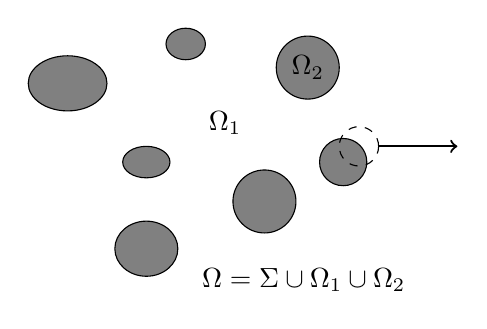
\begin{tikzpicture}
        \foreach \x/\y/\ra/\r in {
        1/3/0.2/0.25,
        2.55/2.7/0.4/0.4,
        0.5/0.4/0.35/0.4,
        2/1/0.4/0.4,
        3/1.5/0.3/0.3,
        0.5/1.5/0.2/0.3,
        -0.5/2.5/0.35/0.5}{
            \draw[fill=gray](\x,\y) ellipse(\r cm and \ra cm);
        }
        \draw[dashed](3.2,1.7)circle(0.25);
        % \draw[thick,->](3.2,1.7)++(0.1767,0.1767)--++(0.4,0.4)--++(1,0);
        \draw[thick,->](3.2,1.7)++(0.25,0)--++(1,0);
        \draw(2.55,2.7)node{$\Omega_2$};
        \draw(1.5,2)node{$\Omega_1$};
        \draw(2.5,0)node{$\Omega = \Sigma \cup \Omega_1 \cup \Omega_2$};
        % \draw(2.5,-1)node{$\Sigma = \sum_\alpha \Sigma_\alpha$};
        % \draw(2.5,-0.5)node{$\Omega_2 = \sum_\alpha \Omega_\alpha$};
    \end{tikzpicture}
    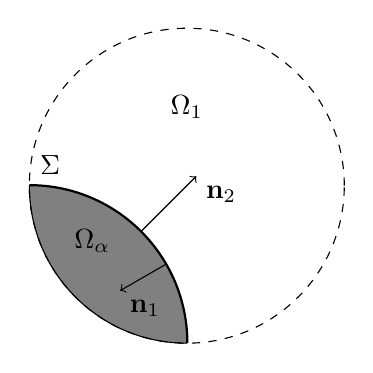
\begin{tikzpicture}%[scale = 0.9]
        \draw[very thick](0:2)arc(0:90:2)node[above right]{$\Sigma$};
        \draw[fill=gray](0:2)arc(0:90:2)arc(180:270:2);
        \draw[dashed](2,2)circle(2);
        \draw[->](1.42,1.42)--++(0.7,0.7)node[below right]{$\textbf{n}_2$};
        \draw[->](1.73,1)--++(-0.577,-0.333)node[below right]{$\textbf{n}_1$};
        \draw(2,3)node{$\Omega_1$};
        \draw(0.8,1.3)node{$\Omega_\alpha$};
    \end{tikzpicture}
    \caption{Scheme of the topology of dispersed two phase flows.}
    \label{fig:Scheme}
\end{figure}
From now on the $k$ indies will refer to either the phase $1$ or $2$, and we drop the time and position arguments in each functions. 
Then, the transport equation of $\chi_k$ can be written as \citep{drew1983mathematical,kataoka1986local,morel2015mathematical},
\begin{equation}
    \pddt \chi_k
    + \textbf{u}_I \cdot \nablabh \chi_k
    = 0,
    \label{eq:dt_chi_k}
\end{equation}
where $\textbf{u}_I$ is the velocity of $\Sigma(t)$.
Besides, it can be shown \citep{tryggvason2011direct,drew1983mathematical,kataoka1986local,bothe2022sharp} that,
\begin{equation}
    \nablabh \chi_k
    = - \delta_I \textbf{n}_k
    \label{eq:grad_chi_k}
\end{equation}
where we have introduced the Interface Indicator Function (IIF) defined as $\delta(\textbf{y}-\textbf{y}_I)$, with $\delta$ being the Dirac-delta function and $\textbf{y}_I$ the position vectors lying on the domain $\Sigma(t)$.
We also define $\textbf{n}_k$ as the outward normal vector of the domain $\Omega_k$.
Taking the gradient of \ref{eq:dt_chi_k} yields the IIF transport equation namely,
\begin{equation}
    \pddt \delta_I
    + \nablabh \cdot \left[(\textbf{u}_I\cdot\textbf{n})\textbf{n} \delta_I\right]
    = \delta_I (\textbf{u}_I\cdot\textbf{n})(\nablabh \cdot\textbf{n})
\end{equation}
As pointed out by \citet{morel2007surface}, it is more convenient to rewrite this equation under the following form,
\begin{equation}
    \pddt \delta_I
    + \nablabh \cdot (\delta_I \textbf{u}_I)
    = \delta_I \nablabhI \cdot \textbf{u}_I.
    \label{eq:dt_delta_I}
\end{equation}
where we introduced the surface divergence operator defined as $\nablabhI \cdot ()= (\textbf{I}-\textbf{nn})\cdot \nablabh \cdot ()$.
Likewise, we can derive an expression for the gradient of $\delta_I$ by taking the gradient of \ref{eq:grad_delta_I} yielding,
\begin{equation}
    % &
    \nablabh\delta_I 
    = \textbf{n} \cdot \nablabh (\textbf{n} \delta_I),
    % &
    % \pddt\delta_I 
    % = - \textbf{n} \cdot \nablabh (\textbf{u}_I  \cdot \textbf{n} \delta_I)
    \label{eq:grad_delta_I}
\end{equation}


Let $f_k(\textbf{y})$ being a volumetric property of the flow solely defined in $\Omega_k(t)$.
Likewise, let $f_I(\textbf{y})$ be an arbitrary surface property defined on $\Sigma(t)$.
Then it is possible to derive the local conservation equations for volumetric and surface quantities \citep{bothe2022sharp,morel2015mathematical,tignol1986modelisation}, using Reynolds transport theorem  and divergence theorem on an arbitrary control volume.
These conservation laws read as, 
\begin{align}
    \label{eq:dt_f_k}
    \pddt f_k
    &= \nablabh \cdot \left(
        \bm{\Phi}_k
        - f_k\textbf{u}_k
        \right)
    + \textbf{S}_k
    & \text{ in } \Omega_k,&\\
    \pddt f_I  
    &= 
    \nablabhI \cdot (\mathbf{\Phi}_{I||} - f_I \textbf{u}_I)
    + \textbf{S}_I
    - \Jump{
        f_k (\textbf{u}_I - \textbf{u}_k)
        + \mathbf{\Phi}_k
     } 
    & \text{ on } \Sigma&
    \label{eq:dt_f_I}
\end{align}
for respectively the volumetric and surface properties.
In \ref{eq:dt_f_I} we introduced the notation $\Jump{\ldots}$ to indicate the sum over both phases, i.e. $\sum_{k=1}^2 [\ldots] \cdot \textbf{n}_k$. 
Where we introduced $\bm{\Phi}_k$ and $\bm{\Phi}_I$ as the non-conservative flux tensor corresponding to $f_k$ and $f_I$. 
The non-conservative flux is often expressed through a constitutive equation depending on the nature of the flow such as the stress tensor for the momentum.
$\textbf{S}_k$ and $\textbf{S}_I$ is defined as the volumetric source term of respectively the phase $k$ and at the interface $\Sigma$.
It is important to notice that \ref{eq:dt_f_k} and \ref{eq:dt_f_I} are solely defined in respectively $\Omega_k$ and $\Sigma$, therefore these equations are referred as local conservation equations.

To generalize these equations over the domain $\Omega$ we follow the formalism of \citet{drew1983mathematical,marle1982macroscopic} and \citet{kataoka1986local} for the volumetric quantities.
Indeed, to any local quantities $f_k$ defined in $\Omega_k$, we assign the field $\chi_k f_k$ which is defined in $\Omega$. 
Similarly, for any local surface quantities $f_I$ defined on $\Sigma$ we assign the field quantity $\delta_I f_I$ defined on $\Omega$. 
Then, multiplying \ref{eq:dt_f_k} and \ref{eq:dt_f_I} by respectively $\chi_k$ and $\delta_I$, and making use of \ref{eq:dt_chi_k} and \ref{eq:dt_delta_I} gives, 
\begin{align}
    \pddt (\chi_k f_k)
    &= \nablabh \cdot (\chi_k \bm{\Phi}_k - \chi_k f_k \textbf{u}_k)
    + \chi_k \textbf{S}_k
    + \delta_I\left[
        \bm{\Phi}_k
        + f_k
        \left(
            \textbf{u}_I
            - \textbf{u}_k
        \right)
    \right]
    \cdot \textbf{n}_k ,
    % & \forall \textbf{y} \in \Omega&
    \label{eq:dt_chi_k_f_k}\\
    \pddt (\delta_If_I)  
    &= 
    \nablabh \cdot (\delta_I \mathbf{\Phi}_{I||} - \delta_I f_I \textbf{u}_I)
    +\delta_I\textbf{S}_I 
    - \delta_I \Jump{
    f_k (\textbf{u}_I - \textbf{u}_k)
    + \mathbf{\Phi}_k
    }.
    \label{eq:dt_delta_I_f_I}
\end{align}
We obtained $k$'s equations defined over the domain $\Omega$ for the bulk quantities, and third global equations for the surface quantities also valid over $\Omega$. 
The transformation of these equations from local to global conservation makes appear a term on the RHS of \ref{eq:dt_chi_k_f_k} representing the interfacial transfer of $f_k$ and $\mathbf{\Phi}_k$, while the surface transport equation did not change fundamentally. 
The set of equations formed by \ref{eq:dt_chi_k_f_k} for $k =1,2$ is commonly known as the \textit{two-fluid} formulation of multiphase flows, to which we add the \textit{jump condition} across the phase given by \ref{eq:dt_delta_I_f_I} \citep{morel2015mathematical,tryggvason2011direct,drew1983mathematical,kataoka1986local}. 
In this work, we prefer to think of those equations as a set of three equations, formed by \ref{eq:dt_chi_k_f_k} for the volumetric conservation equations and \ref{eq:dt_delta_I_f_I} for the surface conservation equations. 

Now that we properly defined the volumetric and surface conservation laws over $\Omega$, let's derive of two phase flows.
We now define any bulk quantity $f$ as $f = \sum_k \chi_k f_k + \delta_I f_I$.
Then adding \ref{eq:dt_chi_k_f_k} for $k=1,2$ and \ref{eq:dt_delta_I_f_I} give the commonly known as the \textit{single-fluid} formulation,
\begin{equation}
    \pddt f
    = \nablabh \cdot (\bm{\Phi} - f \textbf{u})
    + \textbf{S}.
    \label{eq:dt_f}
\end{equation}
Actually, it is more common in the literature to define the bulk quantities as $f = \sum_k \chi_k f_k$ and consider the interfacial terms as source terms as it is often neglected \citep{morel2015mathematical,tryggvason2011direct}. 
Nevertheless, in this work we consider a general case without approximation therefore it is more convenient to think of the bulk quantities as a sum of three phase quantities. 

\subsection{The averaged conservation equations}
\label{sec:avg_def}
In this study, we employ the ensemble average technique to establish the averaged conservation equations. 
This method is just one of several averaging approaches, including the volume average method \citep{jackson1997locally} and time averaging \citep{ishii2010thermo}. 
Despite their differences, all these techniques yield the same set of averaged equations \citep{jackson1997locally,zhang1997momentum}.
In the following we recall some properties of the ensemble average operator. 
Let, $P(\FF)$ be the probability density function that describes the probability of finding the flow in the configuration $\FF$. 
We note $d\PP = P(\FF) d\FF$ the probable number of flows located in the incremental region of the phase space $d\FF$ around the point $\FF$. 
It follows from this definition, that the ensemble average of an arbitrary local property $f^0(\textbf{x},t;\FF)$ defined on the whole space $\Omega$, is,
\begin{equation}
    f(\textbf{x},t)
    = \avg{f^0}(\textbf{x},t)
    =\int f^0(\textbf{x},t;\FF) d\mathscr{P}. 
    \label{eq:avg}
\end{equation}  
Note that we dropped the super script $^0$ on $f(\textbf{x},t)$ to indicate that this is an averaged quantity. 
The macroscopic variables are averaged over all $\FF$, and therefore depend only on $\textbf{x}$ and $t$.
Thus, we omit the arguments of the averaged fields, as this notation eliminates any potential ambiguity. 
The ensemble average quantities are assumed to satisfy the following properties \citep{drew1983mathematical}
\begin{align}
    \label{eq:avg_properties}
    \avg{f^0+h^0} &= f+h, \\ 
    \avg{\avg{f^0}h^0} &= fh, \\
    \avg{\pddt f^0} 
    &= \pddt f, \\ 
    \avg{\grad f^0}
    &= \grad f. 
\end{align}
were $f$ and $h$ are two arbitrary Eulerian fields. 
The first two relations are called the Reynolds' rules, the third one is the Leibniz' rule and the last one, is the Gauss' rule \citep{drew1983mathematical}.
Additionally, for any phase quantity defined in $\Omega_k$ we introduce the definition, 
\begin{equation}
    \phi_k f_k (\textbf{x},t) = \avg{\chi_k f_k^0},
    \label{eq:1_avg}
\end{equation}
where $\phi_k(\textbf{x},t) = \avg{\chi_k}$ is the volume fraction of the phase $k$.
And $f_k$ is the average of the field $f_k^0$ conditioned on the presence of the phase $k$ in the configuration $\FF$ at $\textbf{x}$ and time $t$.
Equally, for interface quantities we have 
\begin{equation}
    \phi_I f_I (\textbf{x},t) = \avg{\delta_I f_I^0},
\end{equation}
with $\phi_I = \avg{\delta_I}$ the interfacial area concentration function. 
Here, $f_I$ is the average of $f^0_I$ conditioned on the presence of an interface in the configuration $\FF$ at $\textbf{x}$ and time $t$. 
Additionally, we define the field of fluctuation of a given quantity around its mean as,
\begin{align}
    f'(\textbf{x},t,\FF) = f^0(\textbf{x},t,\FF) - f(\textbf{x},t).
    \label{eq:def_fluctu}
\end{align}
This relation applies to phase averaged quantities such that $f'_k = f^0_k - f_k$ and $f'_I = f^0_I - f_I$. 


Applying the ensemble average on \ref{eq:dt_chi_k_f_k} and \ref{eq:dt_delta_I_f_I} and considering the properties from \ref{eq:avg_properties} to \ref{eq:def_fluctu}, yields the general form of the averaged equations of multiphase flows, namely,
\begin{align}
    \pddt (\phi_k f_k)
    +\div (\phi_k f_k \textbf{u}_k - \mathbf{\Phi}_k^\text{eq})
    &= 
    \phi_k s_k
    + \avg{\delta_I\left[
        \mathbf{\Phi}_k^0
        + f_k^0
        \left(
            \textbf{u}_I^0
            - \textbf{u}_k^0
        \right)
    \right]
    \cdot \textbf{n}_k} ,
    \label{eq:avg_dt_chi_f}\\
    \pddt (\phi_I f_I)
    +\div (\phi_I f_I \textbf{u}_I- \mathbf{\Phi}_{I}^\text{eq})
    &= 
    \phi_I s_I
    - \avg{\delta_I 
    \Jump{
    f_k^0 (\textbf{u}_I^0 - \textbf{u}_k^0)
    + \mathbf{\Phi}_k^0
    } 
     },
    \label{eq:avg_dt_delta_f}
\end{align}
with, 
\begin{align*}
    \mathbf{\Phi}_k^\text{eq}
    = \avg{\chi_k f_k' \textbf{u}_k'}
    - \phi_k \bm\Phi_k,
    &&
    \mathbf{\Phi}_{I}^\text{eq}
    = \avg{\delta_I f_I' \textbf{u}_I'}
    - \phi_I \bm\Phi_I. 
\end{align*}
These equations are to be solved for the averaged field $\phi_k,\phi_I,f_k$ and $f_I$ with a complementary equation of volume conservation, i.e. $\phi_f+\phi_d+\phi_I = 1$.
The main differences between these equations and their microscale counterparts (\ref{eq:dt_f_k} and \ref{eq:dt_f_I}) are:
(1) The unknowns are now averaged quantities,
(2) Factors $\phi_k$ and $\phi_I$ are introduced in front of all the terms, and
(3) The additional terms $\avg{\chi_k f_k' \textbf{u}_k'}$ and $\avg{\delta_I f_I' \textbf{u}_I'}$ appear, representing the covariance between the conserved quantity ($f_k$ or $f_I$) and the local velocities.  
For a complete understanding, we derived the mass, momentum, and energy averaged equations in \ref{ap:two-fluid_model}. 
These are derived considering the simplifying hypothesis exposed in \ref{ap:hypothesis}. 
In addition, \ref{ap:two-fluid_model} presents how to derive the secondary averaged equations of the averaged energy $E_k$, i.e. the equation for the mean internal energy $e_k$, the pseudo turbulent energy $k_k = \frac{1}{2\phi_k}\avg{\chi_k (u'_k)^2}$, and the averaged kinetic energy $(u_k)^2/2$.  


It is important to highlight that the two-fluid model fails to adequately distinguish between the two phases, as evidenced by the \textit{symmetry} $k = 1$ and $2$ in the aforementioned equations. This symmetry does not hold physically because the dispersed phase possesses a distinct topological nature compared to the continuous phase. 
More importantly, in a dispersed two-phase flow system the closure terms are expressed as a function of the Lagrangian properties of the particles whereas this system of equation provides us with continuously averaged quantities. 
Specifically, the mean drag force or torque term in the averaged momentum equation is expressed as a function of the center of mass linear and angular velocity  of the particles. 
Whereas this system of equation provides us with the phase averaged velocity of the whole phase not with no consideration for the particles properties.  
Therefore, in the subsequent section, we will introduce a kinetic model specifically devoted to the dispersed phase. 
As illustrated below, the equations governing the dispersed phase are more comprehensive as they bear a resemblance to the equations governing a single particle.



In this section, we present a Lagrangian-based model capable of describing the dispersed phase with an arbitrary order of accuracy.

\subsection{Fundamental properties}

At this stage, we define some fundamental properties associated to each particle labeled $\alpha$.
Following the strategy of \citet{lhuillier2009rheology,lhuillier1992volume,zaepffel2011modelisation} and \citet[Chapter 2]{morel2015mathematical}
we define the mass $m_\alpha$, position of center of mass $\mathbf{x}_\alpha$, and the momentum $\textbf{p}_\alpha$ of the particle $\alpha$, as
\begin{align}
    m_\alpha(t,\FF)
    = \intO{ \rho_d  }, 
    &&
    \textbf{x}_\alpha(t,\FF)
    = \frac{1}{m_\alpha(t,\FF) }\intO{ \rho_d \textbf{x} }, 
    &&\textbf{p}_\alpha(t,\FF) 
    = \intO{ \rho_d \textbf{u}_d^0 }.
    \label{eq:mass_pos}
    % \label{eq:momentum_energy}
\end{align}
$\Omega_\alpha(t,\FF)$ is the time-dependent domain occupied by the particle $\alpha$ (see \ref{fig:Scheme}). 
Subsequently, we define the velocity of the particle center of mass as
\begin{equation*}
\textbf{u}_\alpha = \frac{d \textbf{x}_\alpha}{dt}.
\end{equation*}
Replacing $\textbf{x}_\alpha$ by its definition (\ref{eq:mass_pos}) we obtain
\begin{equation*}
    \textbf{u}_\alpha = \frac{1}{m_\alpha}
    \frac{d}{dt} 
    \left(
        \intO{ \rho_d \textbf{x} }
    \right)
    - \frac{1}{m_\alpha^2} \frac{d}{dt} \left(\intO{ \rho_d } \right)
    \intO{ \rho_d \textbf{x} }.
\end{equation*}
%\tb{ A finaliser
Using the Reynolds transport theorem (\ref{eq:reynolds_transport}) for both terms in parentheses and making use of the conservation of mass (\ref{eq:dt_rho}) and the definition of $\textbf{x}_\alpha(t,\FF)$ in the last term, gives
\begin{equation}
    \textbf{u}_\alpha = 
    \frac{1}{m_\alpha}\intO{ \left[
        \pddt (\textbf{x}\rho_d ) + \div\left(\textbf{u}_d \textbf{x} \rho_d\right) 
    \right]} \\
    + \frac{1}{m_\alpha}\intS{ \textbf{x} \rho_d(\textbf{u}_I   - \textbf{u}_d) \cdot \textbf{n}_d }
    -  \frac{\textbf{x}_\alpha}{m_\alpha}    \intS{ \rho_d(\textbf{u}_I   - \textbf{u}_d) \cdot \textbf{n}_d }
\end{equation}
Then by considering the mass conservation for the first term and noticing that $\grad \textbf{x} = \bm\delta$, for the second term gives, 
\begin{equation}
    \textbf{u}_\alpha(t,\FF) = \frac{1}{m_\alpha(t,\FF)} \left(
        \textbf{p}_\alpha(t,\FF)
        +  \intS{\rho_d \textbf{r} (\textbf{u}_I^0 - \textbf{u}_d^0)\cdot \textbf{n}_d }
        \right),
        \label{eq:dt_y_alpha}
\end{equation}
where $\textbf{r}(\textbf{x},t) = \textbf{x} - \textbf{x}_\alpha(t)$. 
In \ref{eq:dt_y_alpha}, it can be observed that the first component of the velocity represents the linear momentum divided by the mass of the particle. 
This corresponds to the mass-averaged velocity over the volume of the particle.
The second term in \ref{eq:dt_y_alpha} arises from the contribution of anisotropic mass transfer across the surface of the particle. 
This mass transfer leads to the motion of the particle's center of mass, thereby contributing to the total velocity.
To illustrate this concept, let us consider a fixed drop with no momentum lying over a very hot plate.
In this scenario, we assume that the plate is sufficiently hot to induce evaporation, specifically on the bottom portion of the drop.
Hence, under the effect of an anisotropic evaporation flux one may expect the second term to be non-negligible.
Consequently, the center of mass of the drop has a non-zero velocity in the opposite direction of the plate, even though the momentum is assumed to be zero.
Note that \ref{eq:dt_y_alpha} generalized usual expression of the center of mass velocity whom neglect the second term.
In the following, for the sake of brevity we discard the dependency on $t$ and $\FF$ on the notations for all Lagrangian quantities denoted by the subscript $_\alpha$ and in particular $\Gamma_\alpha$ and $\Omega_\alpha$.
Nevertheless, the reader must understand that all Lagrangian quantities and integration domains subscribed by $_\alpha$ are time and configuration-dependent. 

The particle's internal relative motions or the \textit{inner velocity} is given by $\textbf{w}_d^0 = \textbf{u}_d^0 - \textbf{u}_\alpha$. 
Substituting the inner velocity in the momentum definition (\ref{eq:mass_pos}) yields
\begin{equation}
    \label{eq:momentum_definition_1}
    \textbf{p}_\alpha
    = m_\alpha \textbf{u}_\alpha
    + \int_{\Omega_\alpha} \rho_d \textbf{w}_d^0 d\Omega.
\end{equation}
Alternatively, from \eqref{eq:dt_y_alpha}, we obtain,
\begin{equation}
    \textbf{p}_\alpha
    =  m_\alpha \textbf{u}_\alpha
    - \int_{\Gamma_\alpha} \rho_d\textbf{r}(\textbf{u}_I^0 - \textbf{u}_d^0)\cdot \textbf{n}_d d\Sigma
    \label{eq:momentum_definition}
\end{equation}
Therefore, the momentum of a particle can be seen as a sum of the mean velocity plus the integral of the fluctuation (\ref{eq:momentum_definition_1}), with the latter being equivalent to minus the first moment of mass transfer term (\ref{eq:momentum_definition}).
Indeed, by identification we obtain : $\intO{ \rho_d \textbf{w}_d^0 } = - \intS{  \rho_d\textbf{r} (\textbf{u}_I^0 - \textbf{u}_d^0)\cdot \textbf{n}_d }$. 
Hence, the internal velocity fluctuations within a fluid particle do not contribute to the total linear momentum $\textbf{p}_\alpha$, as long as the anisotropic mass transfer is negligible.  
Only within this simplified context we can consider the classic relation $\textbf{p}_\alpha = m_\alpha \textbf{u}_\alpha$. 

\subsection{Conservation laws}

We assign to a particle indexed, $\alpha$, occupying the domain $\Omega_\alpha$ (see \ref{fig:Scheme}) an arbitrary Lagrangian property $q_\alpha$ defined by $q_\alpha  = \intO{ f_d^0}$.
Similarly, we define $q_{I\alpha} = \intS{ f_I^0}$ as an integrated surface property of the particle $\alpha$.

\subsubsection{Inside the volume}
To describe the evolution of any arbitrary Lagrangian quantity $q_\alpha$, we need to establish its time derivative.
Since $q_\alpha$ is an integral quantity with a time-dependent domain of integration, we apply the general Reynolds transport theorem for volume integral which gives for material domains (here the droplet volume),
\begin{equation}
    \ddt  \intO{f_d^0}
    = \intO{\left[ \pddt f_d^0 + \div\left(f_d^0\textbf{u}_d^0\right) \right]}\\
    + \intS{ f_d^0 (\textbf{u}_I^0-\textbf{u}_d^0)\cdot \textbf{n}_d }.
    \label{eq:reynolds_transport}
\end{equation}
By substituting the integrand of the first integral on the right-hand side (RHS) with \ref{eq:dt_f_k} we obtain the conservation law of the quantity $q_\alpha$, namely,  
\begin{equation}
    \ddt{q_\alpha}
    = \intO{ s_d^0 }
    + \intS{ \left[
        f_d^0 (\textbf{u}_I^0-\textbf{u}_d^0) 
        + \mathbf{\Phi}_d^0 
        \right] \cdot \textbf{n}_d }.
    \label{eq:dt_q_alpha}
\end{equation}
In \ref{eq:dt_q_alpha} we used the Gauss divergence theorem to show that
\begin{equation}
    \intO{\div \mathbf{\Phi}_d^0} = \intS{\mathbf{\Phi}_d^0 \cdot \textbf{n}_d}.
\end{equation}
The first term on the right-hand side of \ref{eq:dt_q_alpha} accounts for the total contribution of the source term $s_d^0$ to the particle $\alpha$,
while the second term is the surface integration of the exchange terms, which includes the phase transfer flux $f_d^0 (\textbf{u}_I^0-\textbf{u}_d^0)$ and the diffusive flux $\mathbf{\Phi}_d^0$. 


Let us consider the specific case of the momentum balance, i.e. $q_\alpha = \textbf{p}_\alpha$.
In this situation, \ref{eq:dt_q_alpha} reads
\begin{equation}
    \ddt  \textbf{p}_\alpha
    = \intO{ \rho_d\textbf{g} }
    + \intS{ 
        \left[
        f_d^0 (\textbf{u}_I^0-\textbf{u}_d^0)
         + \bm{\sigma}_d^0%\cdot\textbf{n}_d  
        %+ \mathbf{\Phi}_d^0 
        \right] 
        \cdot \textbf{n}_d },
\end{equation}
% first term reads as $\intO{ \rho_d\textbf{g} }$ 
The first term on the right-hand side represents the total weight acting on the particle $\alpha$, 
the second term represents the total source of momentum due to phase transfer, and it is expressed as, $\intS{ \rho_d \textbf{u}_d^0 (\textbf{u}_I^0-\textbf{u}_d^0)\cdot\textbf{n}_d }$,
and the last term $\intS{ \bm{\sigma}_d^0\cdot\textbf{n}_d }$, represents the resultant of the hydrodynamic forces acting on the surface of the particle.
It is important to notice that under this form, the exchange terms are expressed as integrals of dispersed phase fields denoted by the subscript $_d$.
Nevertheless, depending on the nature of the dispersed phase, these fields may not always be defined.
For rigid particles the stress within the particle $\bm{\sigma}_d^0$ is indeterminate \citep{guazzelli2011}.  
Hence, our objective is to express these exchange terms, in terms of the continuous phase field quantities instead of the dispersed phase fields, i.e. in terms of $\mathbf{\Phi}_f^0$ and $\textbf{u}_f^0$ rather than $\mathbf{\Phi}_d^0$ and $\textbf{u}_d^0$. 

\subsubsection{On the interfaces}
To address this issue in a general manner, let us derive the conservation equation for the integrated surface property $q_{I\alpha} = \intS{f_I^0}$.
To differentiate time-varying surface integrals within time, we make use of the general Leibniz rule, which states that for an arbitrary function $f_I^0$ defined on $\Gamma(t)$ we have the relation \citep{nadim1996concise}
\begin{equation}
    \ddt  \intS{f_I^0 }
    = \intS{ \left[
        \pddt f_I^0
        +   \gradI \cdot (\textbf{u}_I^0f_I^0)
    \right]}.
    \label{eq:surface_derivative}
\end{equation}
Substituting the right-hand side terms of \ref{eq:surface_derivative} with \ref{eq:dt_f_I}, gives,
\begin{equation}
    \ddt  q_{I\alpha}
    = \intS{ 
        s_I^0
    }
    - \intS{
 \Jump{
        f_k^0 (\textbf{u}_I^0 - \textbf{u}_k^0)
        + \mathbf{\Phi}_k^0
    }
    }.
    \label{eq:dt_q_I_alpha}
\end{equation}
We have used the surface divergence theorem applied to closed surfaces \citep{nadim1996concise}, it reads
\begin{equation}
    \intS{\gradI F}
    = 
    \intS{ F \textbf{n} (\div \textbf{n})},
    \label{eq:gauss_surface}
\end{equation} 
where $F$ is an arbitrary field.
This theorem demonstrates that any surface property parallel to the tangential plane of $\Gamma$, such as $\bm\Phi_{I||}$, satisfies the relation $\intS{\divI \bm\Phi_{I||}^0}
= 0$.
This explains why $\bm\Phi_{I||}$ does not appear in \ref{eq:dt_q_I_alpha}. 
\ref{eq:surface_derivative} can be interpreted as the conservation equation for the integrated surface property $f_I^0$, or as the jump condition of the $f^0_k$ integrated on the droplet surface. 
As discussed above we wish to get rid of $\mathbf{\Phi}_d^0$ in \ref{eq:dt_q_alpha}. 
To achieve this, we treat the particle's volume and surface as a unified entity and derive a conservation equation for $q_\alpha^\text{tot} = q_\alpha + q_{I\alpha}$. 
By summing \ref{eq:dt_q_alpha} and \ref{eq:dt_q_I_alpha} we directly obtain 
\begin{equation}
    \ddt  q_\alpha^\text{tot}
    = 
    \intO{ s_d^0 }
    + \intS{ s_I^0 }
    + \intS{ \left[
        f_f^0 (\textbf{u}_I^0-\textbf{u}_f^0) 
        + \mathbf{\Phi}_f^0 
        \right] \cdot \textbf{n}_d }. 
    \label{eq:dt_q_alpha_tot}
\end{equation}
This equation is the general form of the linear conservation law for the quantity $q_\alpha^\text{tot}$.
It applies to any particle immersed into a continuous phase following the local conservation, \ref{eq:dt_f_k} and \ref{eq:dt_f_I}.
We refer to this equation as the zeroth-order conservation equation or the linear conservation law for the particle $\alpha$.

We would like to highlight that due to the consideration of closed surface, the diffusive flux $\mathbf{\Phi}_{I||}^0$, plays no role at all in \ref{eq:dt_q_alpha_tot}.
Therefore, in the case of the linear momentum conservation law, the contribution of the momentum diffusive flux $\bm\sigma_{I||}^0$ exposed in \ref{eq:dt_rhoIu_I}, will not contribute to the momentum balance of a particle, and we obtain the relation 
\begin{equation}
    \ddt  \textbf{p}_\alpha^\text{tot}
    = 
    \intO{ \rho_d^0\textbf{g} }
    + \intS{ \rho_I^0\textbf{g} }
    + \intS{ 
        \left[
        f_d^0 (\textbf{u}_I^0-\textbf{u}_f^0)
        + \bm{\sigma}_f^0
        \right] 
        \cdot \textbf{n}_d }. 
\end{equation}
In this case, note that $\textbf{p}_\alpha^\text{tot} = \intO{\rho^0_d \textbf{u}_d^0}+\intS{\rho^0_I \textbf{u}_I^0}$ is the momentum of the particle's volume and surface. 
The latter might be negligible if the interface has a negligible weight. 
As a consequence, even in the presence of local Marangoni forces or surface viscous stresses (see \ref{eq:surface_fluxes}), the resultant of the surface diffusive fluxes would still cancel out in the linear momentum balance.
This fact has already been demonstrated by \citet{hesla1993note} who showed that the surface tension force does not contribute to the linear and angular momentum balance. 
Here, we have provided the general proof that the interfacial diffusive flux $\mathbf{\Phi}_{I||}^0$, which is present at the local scale according to \ref{eq:dt_f_I}, does not contribute to the zeroth-order conservation law of a particle with a closed surface.

For completeness, we exposed in \ref{ap:particles_eq} a clear derivation of the mass, momentum and total energy equations for a single particle.
The derivation takes place using the same hypothesis as it is exposed in \ref{ap:hypothesis}.
Especially, it is shown that the integration of the kinetic energy jump condition corresponds to the Lagrangian derivative of the particle surface, see \ref{eq:int_u_I2}. 

\subsection{Higher moment equations}

Because $f_d^0$ and $f_I^0$ are not always constant over the volumes and surfaces of the particles, it is interesting to introduce in the first place, the first moment of the quantities $f_d^0$ and $f_I^0$. 
They are defined as
\begin{align}
    &\textbf{Q}_\alpha 
    = \intO{ \textbf{r} f_d^0 },
    &\text{and}&
    &\textbf{Q}_{I\alpha}
    = \intS{ \textbf{r} f_I^0 },
    \label{eq:first_moment_definition}
\end{align}
where we recall that $\textbf{r} = \textbf{x} - \textbf{x}_\alpha$ is the distance between any point inside $\Omega_\alpha$ or $\Gamma_\alpha$, to the center of mass of the particle $\alpha$.
It is then possible to differentiate these moments with respect to time to obtain their conservation laws.
We use the Reynolds transport theorem (\ref{eq:reynolds_transport}) to describe the evolution of $\textbf{Q}_\alpha$ within time. 
It gives, 
\begin{equation*}
    \frac{d}{dt} \textbf{Q}_\alpha
      =  \intO{\left[
        \pddt(  f_d^0\textbf{r})
        + \div \left(  f_d^0 \textbf{r}\textbf{u}_d^0\right)
    \right]} 
    + \intS{  f_d^0 \textbf{r}  (\textbf{u}_I^0-\textbf{u}_d^0)\cdot \textbf{n}_d}
\end{equation*}
The first term on the right-hand side may be rewritten as
\begin{equation*}
\intO{ \left[
        \pddt(\textbf{r}  f_d^0)+ \div \left( \textbf{u}_d^0 \textbf{r} f^0_d\right) 
    \right]}
    = \intO{\textbf{r}\left[
        \pddt f_d^0
        + \div \left(f_d^0 \textbf{u}_d^0\right)
    \right] }
    + \intO{ f_d^0 \left[
        \pddt \textbf{r}
        +(\textbf{u}_d^0 \cdot \grad) \textbf{r}
    \right]}
\end{equation*}
Using \ref{eq:dt_f_k} for the first integral on the right-hand side, and considering the relation,
$  \pddt \textbf{r}
+ (\textbf{u}_d^0 \cdot \grad) \textbf{r}
= - \frac{d}{dt} \textbf{y}_\alpha  + \textbf{u}_d^0 
= \textbf{w}_d^0$,
for the second integral yields 
\begin{align}
    \frac{d}{dt} \textbf{Q}_\alpha
    % &= \intO{\textbf{r} \left[
    %      s_d^0  +  \div \bm\Phi_d^0
    % \right]}
    % +\intO{f_d^0  \textbf{w}_d }
    % + \int_{\Gamma_\alpha} \textbf{r}  f_d^0 (\textbf{u}_I^0-\textbf{u}_d^0)\cdot \textbf{n}_d  d\Sigma,\\
    = \intO{\left( 
        \textbf{r} s_d^0  
        + f_d^0  \textbf{w}_d 
        - \bm\Phi_d^0
    \right) }
    + \int_{\Gamma_\alpha} \textbf{r} \left[
        \bm\Phi_d^0
        + f_d^0 (\textbf{u}_I^0-\textbf{u}_d^0)
    \right]\cdot \textbf{n}_d  d\Sigma.
    \label{eq:dt_Q_alpha}
\end{align}
Where we have used the relation $\intO{\textbf{r}  \div \bm\Phi_d^0 }
= \intS{ \textbf{r} \bm\Phi_d^0 \cdot \textbf{n}_d }
- \intO{ \bm\Phi_d^0 }$. 
\ref{eq:dt_Q_alpha} is the first order moment conservation equation for the particle $\alpha$. 
Following the same procedure, and making use of \ref{eq:surface_derivative}, \ref{eq:gauss_surface} and \ref{eq:dt_f_I}, one can equally show that 
\begin{align}
    \ddt {\textbf{Q}_{I\alpha}}
    &= \intS{ \left(
        \textbf{r}s_I^0
        + f_I^0 \textbf{w}_I^0
        - \mathbf{\Phi}_{I||}^0
    \right) }
    - \intS{\textbf{r} 
    \Jump{\mathbf{\Phi}_k^0
        + f_k^0 (\textbf{u}_I^0 - \textbf{u}_k^0)
    }
    },
    \label{eq:dt_Q_I_alpha}
\end{align}
where $\textbf{w}_I^0 = \textbf{u}_{I||}^0 - \textbf{u}_\alpha$.
In \ref{eq:dt_Q_alpha}, we recognize the first moment of the source term $s_d^0$, the first moment of the diffusive flux term $\bm\Phi_d^0\cdot\textbf{n}_d$ and the first moment of phase exchange term, $f_d^0 (\textbf{u}_I^0-\textbf{u}_d^0)\cdot\textbf{n}_d$. 
Additionally, two supplementary terms appear in \ref{eq:dt_Q_alpha}, namely: the integral of the diffusive flux $\bm\Phi_d^0$, and a term related to the fluctuation of the internal velocity $f_d^0 \textbf{w}_d^0$.
Similar observations can be made for the first moment of surface equation \ref{eq:dt_Q_I_alpha}, as it shares similarities with \ref{eq:dt_Q_alpha}. 
In particular, it is worth noting the presence of the surface diffusive flux $\mathbf{\Phi}_{I||}^0$ in \ref{eq:dt_Q_I_alpha}.
This term will be further discussed in the following. 

For similar reason than the linear conservation equations, we sum \ref{eq:dt_Q_alpha} and \ref{eq:dt_Q_I_alpha} to expresses the conservation equation of the total first moment $\textbf{Q}_\alpha^\text{tot} = \textbf{Q}_\alpha + \textbf{Q}_{I\alpha}$, this yields 
\begin{multline}
    \ddt {\textbf{Q}_\alpha^\text{tot}}
    = \intO{ \left(
        \textbf{r} s_d^0         
        + f_d^0  \textbf{w}_d^0 
        - \mathbf{\Phi}_d^0
    \right) }
    + \intS{ \left(
        \textbf{r}s_I^0
        + f_I^0 \textbf{w}_I^0
        - \mathbf{\Phi}_{I||}^0
    \right) }
    + \intS{ \textbf{r} \left[
        \mathbf{\Phi}_f^0
        + f_f^0 (\textbf{u}_I^0-\textbf{u}_f^0)
    \right]\cdot \textbf{n}_d  }. 
    \label{eq:dt_Q_alpha_tot}
\end{multline}
Likewise, conservation laws can be derived for the $n^{th}$ order moments of volume and surface, i.e. for
\begin{align}
    \textbf{Q}_{\alpha n}
    = \intO{
         \underbrace{\textbf{rr}\ldots \textbf{rr}}_{n\text{ times}}
        f_d^0 },
        && \text{and} &&
    \textbf{Q}_{I\alpha n}
    = \intS{
         \underbrace{\textbf{rr}\ldots \textbf{rr}}_{n\text{ times}}
    f_I^0 },
    \label{eq:Q_n_definition}
\end{align} 
respectively. 
It can be shown that the derivative with time of $\textbf{Q}_{\alpha n}$ and $\textbf{Q}_{I\alpha n}$ do not involve any additional terms than in \ref{eq:dt_Q_alpha} and \ref{eq:dt_Q_I_alpha}, but rather just the $n^{th}$ order moments of the already presented terms.
We provide the full derivation of $\ddt{ \textbf{Q}_{\alpha n}}$ in \ref{ap:Moments_equations}.
In short, these higher order moments describe the distributions of the local quantities $f_d^0$ and $f_I^0$ inside the domain $\Omega_\alpha$ and $\Gamma_\alpha$, respectively.
Consequently, an infinite number of moments would be theoretically necessary to recover the fields $f_d^0$ and $f_I^0$ within $\Omega_\alpha$ and $\Gamma_\alpha$. 
Thus, one can reach an arbitrary order of accuracy upon the knowledge of an arbitrary number of moments for a given quantity.  

\subsection{Discussion}

To gain physical insight into the meaning of the first and higher moment equations, we now consider the case of mass and momentum conservation laws for a particle of arbitrary shape. 
For ease of understanding, we adopt the simplifying hypotheses presented in \ref{ap:hypothesis}. 
This implies that we consider no mass transfer across phases and no surface properties except for surface tension forces.

Following \ref{eq:Q_n_definition} we define the second-order moment of mass and the first-order moment of momentum as respectively,
\begin{equation}
    \textbf{M}_\alpha 
    = \intO{ \rho_d \textbf{r} \textbf{r} }
    \;\;\;\text{and}\;\;\;
    \textbf{P}_\alpha 
    = \intO{ \rho_d \textbf{r} \textbf{u}_d^0 }.
    \label{eq:first_moment_of_momentum_def}
\end{equation}
Note that $\textbf{M}_\alpha$ is analogous to the inertia tensor $\textbf{I}_\alpha$ in solid mechanics, both are related through the expression $\textbf{I}_\alpha = \bm\delta : \textbf{M}_\alpha - \textbf{M}_\alpha$.
For a constant density, the tensor $\textbf{M}_\alpha$ describes the second moment of the volume distribution around the particle center of mass.
Likewise, the tensor $\textbf{P}_\alpha$ describes the first moment of the velocity distribution within the particle volume. 
To provide a clearer physical interpretation of the moment of momentum tensor, we decompose $\textbf{P}_\alpha$ into two distinct parts. 
Namely, 
$\textbf{P}_\alpha = \textbf{S}_\alpha+\textbf{T}_\alpha$, where $\textbf{S}_\alpha$ represents the symmetric part and $\textbf{T}_\alpha$ is the antisymmetric part of $\textbf{P}_\alpha$.
Then, the tensors $\textbf{S}_\alpha$ and $\textbf{T}_\alpha$ correspond respectively to the stretching and angular momentum of the particle $\alpha$. 
The tensor $\textbf{S}_\alpha$ quantifies how fast and in which direction the particle gets elongated or flattened, in other words it represents the mean rate of deformation experienced by the particle.
The tensor $\textbf{T}_\alpha$ is related to the angular momentum of the particle denoted by the pseudo vector $\bm\mu_\alpha = \intO{ \rho_d \textbf{r} \times \textbf{u}_d^0 }$. 
Indeed, both  $\textbf{T}_\alpha$ and $\bm{\mu}_\alpha$ represent the angular momentum and are related through $(\bm{\mu}_\alpha)_i = \epsilon_{ijk} (\textbf{P}_\alpha)_{jk}= \epsilon_{ijk} (\textbf{T}_\alpha)_{jk}$, where $\bm\epsilon$ is the third order alternating unit tensor or Levi-Cita tensor. 
Lastly, we also introduce the scalar $M_\alpha =\frac{1}{3}\bm\delta : \textbf{P}_\alpha = \frac{1}{3}\intO{ \rho_d \textbf{r} \cdot \textbf{u}_d^0 }.$, which quantifies the rate at which the particle is being compressed or expanded.
To better explain the implication of these quantities on the particle kinematics we provide in \ref{eq:scheme}, three schemes representing possible inner velocity fields with their corresponding value of the moment of momentum tensor.
Note that in \ref{eq:scheme} we explicit
\begin{figure}[h!]
    \centering
    \hfill
    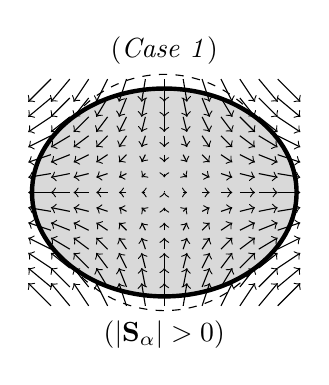
\begin{tikzpicture}[ultra thick,scale=0.6]
        \def\nRows{6}
        \def\nCols{6}
        \draw[dashed,thin] (0,0)circle(2.5);
        \draw[fill=gray!30] (0,0)ellipse(2.8 and 2.2);
        \foreach \x in {-\nRows,...,\nRows} {
            \foreach \y in {-\nCols,...,\nCols} {
                \pgfmathsetmacro\distance{veclen(\x*0.4, \y*0.4)};
                \pgfmathparse{\distance < 2.45 ? "blue" : "white"}
                \edef\colour{\pgfmathresult};
                \ifthenelse{\equal{\colour}{blue}}{                    
                    \draw[thin,->](\x*0.4,\y*0.4)--++(0.08*\x,-0.08*\y);
                }
            }
        }
        \node (txt) at (0,3){(\textit{Case 1})};
        \node (txt) at (0,-3){($|\textbf{S}_\alpha| > 0$)};
    \end{tikzpicture}
     \hfill
    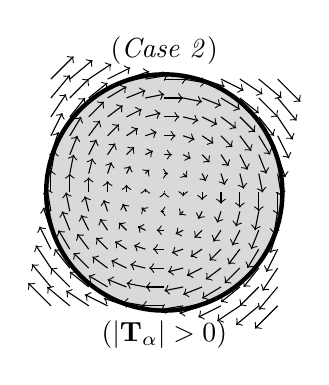
\begin{tikzpicture}[ultra thick,scale=0.6]
        \def\nRows{6}
        \def\nCols{6}
        \draw[fill=gray!30] (0,0)circle(2.5);
        \foreach \x in {-\nRows,...,\nRows} {
            \foreach \y in {-\nCols,...,\nCols} {
                \pgfmathsetmacro\distance{veclen(\x*0.4, \y*0.4)};
                \pgfmathparse{\distance < 2.5 ? "blue" : "white"}
                \edef\colour{\pgfmathresult};
                \ifthenelse{\equal{\colour}{blue}}{                    
                    \draw[thin,->](\x*0.4,\y*0.4)--++(0.08*\y,-0.08*\x);
                }
            }
        }
        \node (txt) at (0,3){(\textit{Case 2})};
        \node (txt) at (0,-3){($|\textbf{T}_\alpha| > 0$)};
    \end{tikzpicture}
    \hfill
    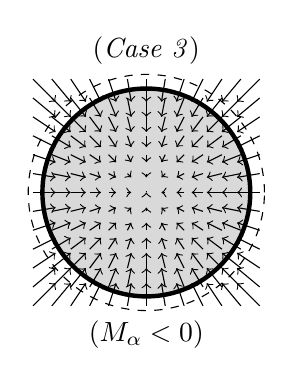
\begin{tikzpicture}[ultra thick,scale=0.6]
        \def\nRows{6}
        \def\nCols{6}
        \draw[dashed,thin] (0,0)circle(2.5);
        \draw[fill=gray!30] (0,0)circle(2.2);
        \foreach \x in {-\nRows,...,\nRows} {
            \foreach \y in {-\nCols,...,\nCols} {
                \pgfmathsetmacro\distance{veclen(\x*0.4, \y*0.4)};
                \pgfmathparse{\distance < 2.3 ? "blue" : "white"}
                \edef\colour{\pgfmathresult};
                \ifthenelse{\equal{\colour}{blue}}{                    
                    \draw[thin,->](\x*0.4,\y*0.4)--++(-0.08*\x,-0.08*\y);
                }
            }
        }
        \node (txt) at (0,3){(\textit{Case 3})};
        \node (txt) at (0,-3){($M_\alpha < 0$)};
    \end{tikzpicture}
    \hfill
    \caption{Graphical representation of the inner kinematics of an arbitrary particle under three scenarios. 
        The arrows represent the velocity field inside the particle, $\textbf{w}_d^0$, with the corresponding value of the moment of momentum tensor indicated below. 
        The operator $|\ldots|$ refers to the norm of the tensors. 
        According to the inner velocity field:
        (\textit{Case 1}) The particle experiences a mean rate of deformation, resulting in non-zero stretching of momentum along the principal axis of deformation;
        (\textit{Case 2}) The particle is rotating, leading to a non-zero angular momentum vector in the direction of rotation;
        (\textit{Case 3}) The particle undergoes compression, resulting in a negative trace of the moment of momentum.
    }
    \label{eq:scheme}
\end{figure}

Injecting, $f_d^0 = \rho_d$ in the second-order moment equation (derived in \ref{ap:Moments_equations}) we obtain :
\begin{equation}
    \ddt {\textbf{M}_\alpha}=2\textbf{S}_\alpha. 
    \label{eq:dt_M_alpha}
\end{equation}
which is the second-order moment of mass conservation equation. 
From \ref{eq:dt_M_alpha} we deduce that the evolution of the distribution of mass of a particle is solely motivated by the stretching of momentum $\textbf{S}_\alpha$. 
This implies that the angular momentum (not to be confused with the angular velocity) plays no role in the evolution of the second moment of mass. 
This is due to the symmetry of the tensor $\textbf{M}_\alpha$, which must be preserved after differentiation with respect to time.
Note that if the particle has a constant $\textbf{M}_\alpha$ under change of reference frame, such as for spherical particles where we can write $\textbf{M}_\alpha= \frac{a^2 m_\alpha}{5} \bm\delta$, then $\textbf{S}_\alpha=0$ since $\ddt \textbf{M}_\alpha = 0$ in this situation.
This argument has no restriction on the internal particle motions, thus it is also true for fluid particles with possible inner motion. 
Additionally, applying the trace operator on both sides of \ref{eq:dt_M_alpha}, yields the interesting relation $\ddt {M_\alpha}=\frac{2}{3}\bm\delta : \textbf{S}_\alpha$.
We can state that $M_\alpha = \lambda^\alpha_1(t)+\lambda^\alpha_d(t)+\lambda^\alpha_3(t)$, with $\lambda_i^\alpha$ for $i=1,2,3$, the eigenvalues of $\textbf{M}_\alpha$, as it is a symmetric tensor and thus always diagonalizable.
For undeformable particles, it is evident that the eigenvalues are not functions of time, implying $\ddt M_\alpha = 0$.  
Consequently, $\bm\delta : \textbf{S}_\alpha$ possesses the notable property of being zero whenever the particle shape remains constant, regardless of the orientation.

Now that we have described the kinematics of the particle shape, let us proceed to derive an equation for the dynamics of the particle shape, i.e. an equation for the moment of momentum. 
This equation is derived injecting $\textbf{Q}_\alpha = \textbf{P}_\alpha$ in \ref{eq:dt_Q_alpha_tot}, it reads, 
\begin{equation}
    \ddt {\textbf{P}_\alpha}
    - \intO{ \rho_d  \textbf{w}_d^0 \textbf{w}_d^0 }
    = 
    - \intO{\bm{\sigma}_d^0}
    - \intS{ 
        \gamma (\bm\delta - \textbf{nn})
    }
    + \intS{ \textbf{r}\bm{\sigma}_f^0\cdot \textbf{n}_d}.
    \label{eq:dt_P_alpha}
\end{equation}
On the left-hands side of \ref{eq:dt_P_alpha} we identify two inertial terms, i.e. the derivative of $\textbf{P}_\alpha$ and the internal velocity term $\intO{\rho_d\textbf{w}_d^0\textbf{w}_d^0 }$.
The inertia of the particle is then balanced by the terms on the right-hand side of the equation, namely: 
the integral of the particle internal stress $\intO{ \bm{\sigma}_d^0}$; 
the integral of the surface tension stress $\intS{ \gamma (\bm\delta- \textbf{nn}) }$; 
and the first moment of the hydrodynamic stress tensor, $\intS{\textbf{r}\bm\sigma_f^0\cdot \textbf{n}}$.
A discussion regarding the physical implications of this equation is provided below. 

The conservation equation of the angular momentum $\bm{\mu}_\alpha$ is obtained by taking the double contracted product of \ref{eq:dt_P_alpha} with $\bm\epsilon$, which gives 
\begin{equation}
    \ddt\bm{\mu}_\alpha
    =  
    % \textbf{t}_\alpha.
    \intS{ \textbf{r} \times \bm{\sigma}_f^0\cdot \textbf{n}_d }
    \label{eq:dt_mu_alpha}
\end{equation}
Notice that every term on the right-hand side of \ref{eq:dt_P_alpha} vanished due to their symmetric nature apart from the shew-symmetric part of the hydrodynamic stress, which is the hydrodynamic torque applied on the particle $\alpha$.
Particularly, the surface tension terms do not appear in the angular momentum balance since $\bm\sigma_I^0 = \gamma (\bm\delta-\textbf{nn})$ is symmetric, which is consistent with the findings of \citet{hesla1993note}. 
As a consequence, the surface tension does not affect the angular momentum regardless of the particle's shape. 
In the literature, it is common to include the torque due to inter-particular interactions in the angular momentum balance, as is done in \citet{jackson1997locally} and \citet{zhang1997momentum}.
In our case note that $\bm{\sigma}_f^0$ contains also short-range interaction forces which can be assimilated to the particle-particle interaction forces.

Taking the double contracted product of \ref{eq:dt_P_alpha} with the tensor $\bm\delta$ and using \ref{eq:dt_M_alpha}, yields directly  
% \begin{equation}
%     \frac{1}{2}\ddt^2 {M_\alpha}
%     - \frac{1}{3}\intO{ \rho_d \textbf{w}_d^0 \cdot \textbf{w}_d^0}
%     = 
%     \intO{p_d^0} 
%     % - \frac{1}{3}\intS{p_f^0 \textbf{r}\cdot \textbf{n}}
%     - \frac{2}{3} \gamma s_\alpha
%     - \frac{1}{3}\intS{p_f^0 \textbf{r}\cdot \textbf{n}}
%     + \frac{1}{3}\intS{\textbf{r}\cdot\bm\tau_f^0\cdot \textbf{n}},
%     \label{eq:dt_D_alpha}
% \end{equation}
\begin{equation}
    \frac{3}{2}\frac{d^2 M_\alpha}{dt^2}
    - \intO{ \rho_d \textbf{w}_d^0 \cdot \textbf{w}_d^0}
    = 
    - \intO{\bm\sigma_d^0:\bm\delta} 
    % - \frac{1}{3}\intS{p_f^0 \textbf{r}\cdot \textbf{n}}
    - \gamma 2 \intS{}
    % - \frac{1}{3}\intS{p_f^0 \textbf{r}\cdot \textbf{n}}
    + \intS{\textbf{r}\cdot\bm\sigma_f^0\cdot \textbf{n}}.
    \label{eq:dt_D_alpha}
\end{equation}
\ref{eq:dt_D_alpha}, corresponds to the isotropic work balance over the volume and surface of the particle. 
According to \ref{eq:dt_D_alpha}, the rate of compression of a particle, denoted by the second derivative of $M_\alpha$ evolves according to : 
the internal inertial term, $\intO{\rho_d \textbf{w}_d^0 \cdot \textbf{w}_d^0 }$;
the particle internal pressure $\intO{\bm\sigma_d^0:\bm\delta}$; 
the surface energy $\gamma\intS{  }$; 
and the trace of the hydrodynamic first moment $\intS{\textbf{r}\cdot\bm\sigma_f^0\cdot \textbf{n}}$.
If one considers spherical particles composed of compressible fluid, \ref{eq:dt_D_alpha} transforms into the Rayleigh-Lamb-Plesset equation. 
In the steady-state regime, this reduces to the Young-Laplace equation, as indicated by the presence of the first three terms on the right-hand side of \ref{eq:dt_D_alpha}. 

\tb{
    As an example we now consider the \textit{Rayleigh-Lamb-Plesset} equation for spherical bubbles with radius $a_\alpha(t)$. 
    As the droplets remain spherical while keeping a constant mass the moment of momentum and inner velocity field can be expressed, 
    \begin{align*}
        M_\alpha
        = \frac{m_\alpha}{5} a^2_\alpha(t),
        && 
        \textbf{w}_d^0
        = \frac{d a_\alpha}{dt}\frac{\textbf{r}}{a_\alpha(t)},
        \label{eq:expr1}
    \end{align*}
    where it is empathized that the radius $a_\alpha(t)$ is time-dependent. 
    The stress inside the bubbles might be expressed as compressible Newtonian fluids with no resistance to shear such that 
    \begin{equation}
        \bm\sigma_d^0 
        = 
        - p_d^0 \bm\delta
        - \lambda_d (\div \textbf{u}_d^0) \bm\delta
        % + \mu_d \left[\grad \textbf{u}_d^0 + (\grad \textbf{u}_d^0)^\dagger\right]
        = 
        - p_d^0 \bm\delta
        - \frac{3 \lambda_d}{a_\alpha} \frac{d a_\alpha}{dt}  \bm\delta
        % + \mu_d \left[\grad \textbf{u}_d^0 + (\grad \textbf{u}_d^0)^\dagger\right]
        \label{eq:StressBubbles}
    \end{equation}
    where $\lambda_d^0$ is the volume viscosity of the dispersed phase. 
    Assuming incompressible Newtonian fluid for the continuous phase and injecting the expressions \ref{eq:StressBubbles} and \ref{eq:expr1} into \ref{eq:dt_D_alpha} yields, 
    \begin{equation}
        \frac{1}{5} \rho_d^0 a_\alpha \frac{d^2 a_\alpha}{dt^2} 
        - 
        \frac{1}{a_\alpha} \frac{d a_\alpha}{dt} 
        \left(
            3 \lambda_d
            + 2 \mu_f 
        \right)
        = 
        +  \frac{1}{v_\alpha}\intO{p_d^0}
        -  \frac{1}{s_\alpha}\intS{p_f^0}
        - \gamma 2 \frac{3}{a}
    \end{equation}
    By expressing the fluid pressure on the surface in terms of the far field pressure (see daniel) one obtain the \textit{Rayleigh-Lamb-Plesset} equation. 
}

Taking the symmetric part of \ref{eq:dt_P_alpha}, and making use of \ref{eq:dt_M_alpha}, yields a dynamical balance equation for $\textbf{M}_\alpha$, namely
% \begin{multline}    
%     \frac{1}{2}\ddt^2{\textbf{M}_\alpha^\text{dev}}
%     - \intO{\left(
%         \rho_d\textbf{w}_d^0 \textbf{w}_d^0
%         - \rho_d\frac{1}{3}(\textbf{w}_d^0 \cdot \textbf{w}_d^0)\bm\delta\right)}
%     =  
%         - \mu_d \intO{\textbf{e}_d^0}
%         - \intS{\gamma\left(\frac{1}{3}\bm\delta-\textbf{nn}\right)}\\
%         + \frac{1}{2}\intS{\left(\textbf{r}\bm\sigma_f^0+ \bm\sigma_f^0\textbf{r} - \frac{2}{3}(\bm\sigma_f^0\cdot \textbf{r})\bm\delta\right)\cdot \textbf{n}}
%     \label{eq:dt_S_alpha}
% \end{multline}
\begin{equation}    
    \frac{1}{2}\frac{d^2 \textbf{M}_\alpha}{dt^2}
    - \intO{ \rho_d  \textbf{w}_d^0 \textbf{w}_d^0 }
    = 
    - \intO{\bm{\sigma}_d^0}
    - \intS{\gamma (\bm\delta - \textbf{nn})}
    + \intS{(\textbf{r}\bm{\sigma}_f^0+\bm{\sigma}_f^0 \textbf{r})\cdot \textbf{n}_d}.
    \label{eq:dt_S_alpha}
\end{equation}
On the left-hand side of \ref{eq:dt_S_alpha}, we recover the symmetric part of the inertial contributions. 
Especially, in opposition to \ref{eq:dt_P_alpha} we could substitute $\textbf{P}_\alpha+\textbf{P}_\alpha^\dagger$ by $\ddt \textbf{M}_\alpha$. 
Consequently, \ref{eq:dt_S_alpha} is a dynamical equation for the droplet mean deformation. 
In our case, only the external contribution $\frac{1}{2}\intS{\textbf{r}\bm\sigma_f^0\cdot \textbf{n}}$ is responsible for the generation of angular momentum, see \ref{eq:dt_mu_alpha}.
Taking the symmetric part of this tensor ultimately removes this contribution. 
Thus, on the right-hand side of \ref{eq:dt_S_alpha}, we identify the terms responsible for the droplet deformation exclusively.
Therefore, \ref{eq:dt_S_alpha} must be interpreted as an equation for the shape of the particle, represented by the tensor $\textbf{M}_\alpha$.

One might immediately recognize that this equation is in fact an extension of Batchelor’s famous result, 
\begin{equation}
    \intO{\bm{\sigma}_d^0}
    + \intS{\gamma(\bm\delta - \textbf{nn})}
    = \frac{1}{2}\intS{(\textbf{r}\bm\sigma_f^0+\bm\sigma_f^0\textbf{r})\cdot \textbf{n}},
    \label{eq:Batchelor}
\end{equation}
but with the consideration of the inertia of the particle.
\ref{eq:Batchelor} is particularly useful to express the unknown internal stress within solid particles (in which case $\gamma = 0$), in terms of surface integral, i.e. the stresslet $\intS{(\textbf{r}\bm\sigma_d^0+ \bm\sigma_d^0\textbf{r})\cdot \textbf{n}}$.
This relation is the main tool used to express the bulk stress of a suspension, it eventually leads to the computation of the famous Einstein equivalent viscosity, upon having a closed expression for the average of $\intS{(\textbf{r}\bm\sigma_d^0+ \bm\sigma_d^0\textbf{r})\cdot \textbf{n}}$ \citep{guazzelli2011}. 
In the inertial case, due to the limited degree of freedom of solid particles, the tensors $\textbf{M}_\alpha$ and the inner velocity field $\textbf{w}_d^0$ are fully determined by \ref{eq:dt_M_alpha} and \ref{eq:dt_mu_alpha}, indicating that $\textbf{M}_\alpha$ and $\textbf{w}_d^0$ can be utilized in \ref{eq:dt_S_alpha} not as unknowns but as source terms. 
Consequently, for solid particles, \ref{eq:dt_S_alpha} must be interpreted as a generalized equation for the undefined stress $\bm\sigma_d^0$ integrated on the volume of the particles.
Whether it is solid or fluid particles \ref{eq:dt_S_alpha} becomes particularly relevant for expressing the averaged stress within an inertial suspension in terms of Lagrangian properties, as discussed in section \ref{sec:averaged_eq}.

It is now clear that if the surface tension forces play no role in the linear and angular momentum equation, it does impact the moment of momentum $\textbf{P}_\alpha$ or more specifically its symmetric part $\textbf{S}_\alpha$.
Thus, the surface tension force impacts the hydrodynamic behavior of a particle solely through its action on $\textbf{S}_\alpha$, which is related to the shape of a particle represented by $\textbf{M}_\alpha$, through \ref{eq:dt_M_alpha}.
In \ref{ap:Moments_equations} we show how to derive the higher-order moment of momentum equations, which can also be viewed as formulas for the higher moments of the internal particle stress distribution. 
It is interesting to mention that in a recent study of \citet{dolata2021faxen} and \citet{zhou2020lamb} they use energy methods and recover the first two moments of momentum equations hidden into another but equivalent form, valid in the Stokes flow regime. 

Hence, the moment of momentum emerges as a quantity of utmost importance for all types of particles with variable shape or volume. In general, the first moments $\textbf{Q}_{\alpha}$ and $\textbf{Q}_{I\alpha}$ hold significant importance when considering particles with high internal gradients, i.e. when $\grad f_d^0$ or $\gradI f_I^0$ are non-negligible at the scale of one particle. 


Two distinct descriptions can be applied to the dispersed phase, while only one description is applicable to the fluid phase. 
In this section, we derive averaged equations for the dispersed phase using Lagrangian conservation laws. 
Following this, we  discuss the equivalence between the particle or lagrangian averaged equations for the dispersed phase and the averaged equations for the dispersed phase presented in \ref{sec:two-fluid}.


%Two different descriptions are possible for the dispersed phase while one is available for the fluid phase. 
%In this part we first derive averaged equations for the dispersed phase based on Lagrangian conservation laws. 
%Then we provide a complete discussion regarding the equivalence between the "lagrangian" averaged equations for the dispersed phase and the averaged equations governing the dispersed phase presented in \ref{sec:two-fluid}. 
%based on 
%the set of equations just derived and the averaged equations governing the dispersed phase presented in \ref{sec:two-fluid}. 

\subsection{Dispersed phase averaged equations}

In the preceding section, we have described the dispersed phase using a Lagrangian framework. 
However, to ensure consistency with the Eulerian conservation equations that describe the continuous phase, it is necessary to extend the Lagrangian equations to an Eulerian description. 
The approach presented here follows the methodology pioneered by \citep{lhuillier1992ensemble}.
%In the last section, we have described the dispersed phase within a Lagrangian framework.
%However, to be consistent with the Eulerian conservation equations used to describe the continuous phase, we need to extend the Lagrangian equations to an Eulerian description. 
%The strategy exposed here follow the approach pionnered by \citep{lhuillier1992ensemble}.
%In order to achieve this,
We introduce the function $\delta_\alpha$, which is defined as follows, 
\begin{align}
    \delta_\alpha(\textbf{x},\textbf{x}_\alpha(t,\FF)) 
    = \delta(\textbf{x}-\textbf{x}_\alpha(t,\FF)),
    \label{eq:delta_alpha}
\end{align}
where $\delta$ is the Dirac function.
Note that we explicitly note the arguments $(t,\FF)$ to highlight that the position of the particle $\alpha$ is a function of time and of the flow configuration $\FF$.
Applying the chain rule yields \citep{lhuillier1998}%we may write the partial time derivative of $\delta_\alpha$ can be written as
%\begin{equation}
%\frac{\partial \delta_\alpha(\textbf{x},\textbf{x}_\alpha(t,\FF))}{\partial t} 
%=  \frac{\partial \textbf{x}_\alpha}{\partial t} 
%\cdot \frac{\partial \delta_\alpha}{\partial \textbf{x}_\alpha}(\textbf{x},\textbf{x}_\alpha(t,\FF)) .
%\end{equation}
%This leads to the following expression, 
\begin{equation}
    \pddt \delta_\alpha
    + \div (\textbf{u}_\alpha  \delta_\alpha)
    =0,
    \label{eq:dt_delta_alpha}
\end{equation}
where we used the identity, $\frac{\partial \delta_\alpha}{\partial \textbf{x}_\alpha}  = -\grad \delta_\alpha$ and the fact that $\textbf{u}_\alpha(t,\FF)$ is not a function of $\textbf{x}$. 
\ref{eq:dt_delta_alpha} does not apply in scenarios where topological changes occur, such as break-up or coalescence events. 
In these cases, a source term can be introduced on the right-hand side of \ref{eq:dt_delta_alpha}, similar to the approach used in population balance equations, to account for the birth or death of particles \citep{randolph2012theory}.
%It should be noted that \ref{eq:dt_delta_alpha} is not applicable if changes in topology, such as break-up or coalescence events, occur.
%In such cases it is possible, as it is done in population balance equations, to include a source term on the RHS of \ref{eq:dt_delta_alpha} to account for particle birth or death. 
%Multiplying each Lagrangian quantities $\text q_\alpha$ by $\delta_\alpha$ yields the field $\text q_\alpha(t,\FF)\delta_\alpha(\textbf{x},t,\FF)$, which is defined over the entire domain $\Omega$.
%Likewise, for any derivative of Lagrangian quantities, such as $\ddt \text q_\alpha$, we define its corresponding Eulerian field by multiplying $\ddt \text q_\alpha$ with $\delta_\alpha$ and show that :
By multiplying each Lagrangian quantity $\text q_\alpha$​ by $\delta_\alpha$​, we obtain the field $\text q_\alpha(t,\FF)\delta_\alpha(\textbf{x},t,\FF)$, which is defined throughout the entire domain $\Omega$. 
Similarly, for any derivative of a Lagrangian quantity, such as $\ddt \text q_\alpha$​, the corresponding Eulerian field is defined by multiplying $\ddt \text q_\alpha$ with $\delta_\alpha$ 
%This can be expressed as
Given that $\text q_\alpha(t,\FF)$ and $\textbf{u}_\alpha(t,\FF)$ do not depend on \textbf{x}, and by using Equation \ref{eq:dt_delta_alpha}, we obtain
\begin{equation}
    \delta_\alpha \ddt \text q_\alpha
    = \pddt (\delta_\alpha \text q_\alpha)
    + \div (\delta_\alpha \text q_\alpha \textbf{u}_\alpha).
    \label{eq:dt_delta_alpha_q_alpha}
\end{equation}
%where we have used the fact that $\text q_\alpha(t,\FF)$ and $\textbf{u}_\alpha(t,\FF)$ are not function of \textbf{x}, and we made use of \ref{eq:dt_delta_alpha}.
%Now let us consider a domain containing $N$ particles.
%We define what we call the \textit{particle field} of a quantity $\text q_\alpha$, as the sum of the $\delta_\alpha \text q_\alpha$ over all particles in the flow, namely $\displaystyle\sum_{\alpha=0}^N \delta_\alpha \text q_\alpha$.
%Notice that \ref{eq:dt_delta_alpha_q_alpha} remains valid for a sum of fields since derivative and sum operators commute.
Consider a domain containing $N$ particles. We define the \textit{particle field} for a quantity $\text q_\alpha$​ as the sum of $\delta_\alpha \text q_\alpha$ over all particles within the domain, expressed by $\displaystyle\sum_{\alpha=0}^N \delta_\alpha \text q_\alpha$​. 
Note that the formula given by \ref{eq:dt_delta_alpha_q_alpha} remains valid for the sum of such fields, since the operations of differentiation and summation commute.
%In the objective of obtaining averaged equations for the dispersed phase, we introduce the average of $\text q_\alpha$ as  
To obtain the averaged equations for the dispersed phase, we define the particle average of $\text q_\alpha$​ as
\begin{equation}
     n_p \text q_p(\textbf{x},t) = \avg{\sum_\alpha\delta_\alpha \text q_\alpha},
     \label{eq:p_avg}
\end{equation}
where, $n_p(\textbf{x},t) = \avg{\sum_\alpha \delta_\alpha}$ is the probability density of finding a particle center of mass in the infinitesimal volume $d\textbf{x}$ around \textbf{x}, and $\text q_p(\textbf{x},t)$ is the average of $\text q_\alpha$ conditionally on the presence of a particle at \textbf{x} and time $t$. 
To simplify the notations, we consider the shorthand \citep{lhuillier1998},
\begin{equation*}
    \sum_\alpha \delta_\alpha \to \delta_p, 
\end{equation*}
such that $\pavg{\text q_\alpha}=\avg{\sum_\alpha \delta_\alpha \text q_\alpha}=n_p\text q_p$.
Note that we used the subscript $_p$ on $\text q_p$ to denote that this represents a particle-averaged field, initially derived from Lagrangian quantities. 
%Furthermore, in view of equation   
Additionally, in light of \ref{eq:def_fluctu} we define the fluctuating part of a particle field $\text q_p$ as
\begin{equation}
    \text q_\alpha' = \text q_\alpha - \text q_p. 
    \label{eq:def_fluc_p}
\end{equation}

To obtain the particle phase averaged equations one multiply \ref{eq:dt_q_alpha_tot} and \ref{eq:dt_Q_alpha_tot} by $\delta_\alpha$ and apply the ensemble average (\ref{eq:avg}), this yields
\begin{align}
    \pddt (n_p\text Q_p)
    + \div (n_p \text Q_p \textbf{u}_p + \pavg{\textbf{u}_\alpha' \text Q_\alpha'})
    = \pOavg{ s_d^0 }
    + \pSavg{ s_I^0 }\nonumber\\
    + \pSavg{ \left[\mathbf{\Phi}_f^0 + f_f^0 (\textbf{u}_\Gamma^0-\textbf{u}_f^0) \right] \cdot \textbf{n}_d },
    \label{eq:avg_dt_dq_alpha_tot}\\
    \pddt (n_p\textbf{Q}_p^{(1)})
    + \div \left(n_p \textbf{Q}_p^{(1)} \textbf{u}_p + \pavg{\textbf{u}_\alpha' \textbf{Q}_\alpha^{(1)'}}\right)
    =\pOavg{ \left(
        \textbf{r} s_d^0         
        + f_d^0  \textbf{w}_d^0 
        - \mathbf{\Phi}_d^0
    \right) }\nonumber\\
    + \pSavg{ \left(
        \textbf{r}s_\Gamma^0
        + f_\Gamma^0 \textbf{w}_\Gamma^0
        - \mathbf{\Phi}_{\Gamma||}^0
    \right) }
    + \pSavg{ \textbf{r} \left[
        \mathbf{\Phi}_f^0
        + f_f^0 (\textbf{u}_\Gamma^0-\textbf{u}_f^0)
    \right]\cdot \textbf{n}_d  }.
    \label{eq:avg_dt_dQ_alpha_tot}
\end{align}
The derivation of the higher moment particle-averaged equations is provided in \ref{ap:Moments_equations}.
The only fluxes appearing in \ref{eq:avg_dt_dq_alpha_tot} and \ref{eq:avg_dt_dQ_alpha_tot} are the fluctuation tensors $\pavg{\textbf{u}_\alpha' \text q_\alpha'}$ and $\pavg{\textbf{u}_\alpha' \textbf{Q}_\alpha'}$. 
Therefore, the non-convective fluxes $\bm\Phi_d^0$ and $\bm\Phi_I^0$ do not play the role of macroscopic fluxes, as it is the case in \ref{eq:avg_dt_chi_f} and \ref{eq:avg_dt_delta_f}. Instead, they act as source terms in the first moment and higher moment equations. 
This distinction is the main structural differences between the Kinetic-like model (\ref{eq:avg_dt_dq_alpha_tot} and \ref{eq:avg_dt_dQ_alpha_tot}) and the two-phase flow model (\ref{eq:avg_dt_chi_f} and \ref{eq:avg_dt_delta_f}). 
In this study, \ref{eq:avg_dt_chi_f} and \ref{eq:avg_dt_delta_f} are referred to as the phase-averaged equations, while \ref{eq:avg_dt_dq_alpha_tot} and \ref{eq:avg_dt_dQ_alpha_tot} are called the particle-averaged equations. 


 





%\subsubsection*{Equivalence between particle and continuous models}
\subsection{Equivalence between particle-averaged and phase-averaged equations}
\label{sec:equivalence}
%To model the dispersed phase we can either use \ref{eq:avg_dt_chi_f} with $k=d$, or the particle-averaged equations: \ref{eq:avg_dt_dq_alpha_tot}, \ref{eq:avg_dt_dQ_alpha_tot} and possibly the higher moments equations in \ref{ap:Moments_equations}. 
%Consequently, it is fair to address the question of the compatibility and differences between both formalisms. 
To model the dispersed phase, there are two distinct approaches. 
We can either use \ref{eq:avg_dt_chi_f} with $k=d$, or we can employ the particle-averaged equations \ref{eq:avg_dt_dq_alpha_tot}, \ref{eq:avg_dt_dQ_alpha_tot} and potentially the higher moments equations found in \ref{ap:Moments_equations}.
Consequently, it is important to address the compatibility between these two formalisms.
It has been demonstrated in various studies \citep{buyevich1979flow,lhuillier1992ensemble,jackson1997locally,zhang1994averaged}, that phase-averaged quantities can be expressed as a Taylor series expansion of particle-averaged quantities. 

The aforementioned studies used the single-particle conditionally averaged approach to demonstrate this equivalence.  
In this work we use instead the ``distributional'' approach of \citet{pahtz2023general} since, as shown below it yields more general and simpler formulation. 
The dispersed phase indicator function $\chi_d$ can be expressed as a sum of phase indicator function, $\chi_d(\textbf{x},t,\FF) = \sum_\alpha\chi_\alpha(\textbf{x},t,\FF)$ where $\chi_\alpha =1$ in the particle domain $\Omega_\alpha(\FF,t)$ and $0$ otherwise. 
Thus, any dispersed phase quantity pertaining to a single particle can be written as, 
\begin{equation}
   f^0_d \chi_\alpha(\textbf{x},t,\FF)
   = 
   \int_{\mathbb{R}^3} 
    f^0_d \chi_\alpha(\textbf{x}_\alpha + \textbf{r},t,\FF)\delta(\textbf{x} - \textbf{x}_\alpha - \textbf{r}) 
    d\textbf{r} 
   \label{eq:taylor_f_d}
\end{equation}
Likewise, we assume that the interface indicator function $\delta_\Gamma$ can be partitioned into $N$ interface indicator function such that $\delta_\Gamma =  \sum_\alpha  \delta_{\Gamma\alpha}$.
In that case any surface-averaged quantities may be written, 
\begin{equation}
    f_\Gamma^0 \delta_\Gamma(\textbf{x},t,\FF) = 
    \sum_\alpha 
    \int_{\mathbb{R}^3} 
     f_\Gamma^0 \delta_{\Gamma\alpha}(\textbf{x}_\alpha + \textbf{r},t,\FF)\delta(\textbf{x} - \textbf{x}_\alpha - \textbf{r}) 
     d\textbf{r}. 
    \label{eq:taylor_f_I}
\end{equation}
% Notice that \ref{eq:taylor_f_d} and \ref{eq:taylor_f_I} are well-defined in the distributional sense since the integral on the right-hand side of both equations correspond to a convolution product.
Notice that the integral on the right-hand side of \ref{eq:taylor_f_d} and \ref{eq:taylor_f_I} correspond to a convolution product.
Additionally, since the Dirac distribution $\delta(\textbf{x} - \textbf{x}_\alpha - \textbf{r})$, is the unit of convolution \ref{eq:taylor_f_d} is verified (see \citet[Chapter 9]{appel2007}).
The convolution product of the Dirac delta and the derivative of the Heaviside distribution is also well-defined, see \citet[Chapter 9]{appel2007}.
It follows that \ref{eq:taylor_f_d} and \ref{eq:taylor_f_I} are well-defined in the distributional sense. 
Upon using the Taylor expansion of the Dirac delta function $\delta(\textbf{x} - \textbf{x}_\alpha - \textbf{r})$ in the neighborhood of $\textbf{r}=0$ one obtain,
\begin{equation}
\delta(\textbf{x} - \textbf{x}_\alpha - \textbf{r})
= \delta(\textbf{x} - \textbf{x}_\alpha)
- \textbf{r}\cdot\grad \delta(\textbf{x} - \textbf{x}_\alpha)
+ \frac{\textbf{rr}}{2}:\grad\grad\delta(\textbf{x} - \textbf{x}_\alpha) 
- \ldots.
% + \ldots
\label{eq:exp_delta}
\end{equation}
Injecting \ref{eq:exp_delta} into \ref{eq:taylor_f_d} and \ref{eq:taylor_f_I}, and noticing that the indicator functions, $\chi_\alpha$ and $\delta_\Gamma$, reduce the domain of integration from $\mathbb{R}^3$ to, $\Omega_\alpha$ and $\Gamma_\alpha$, respectively,  yields: 
\begin{align}
    f^0_d \chi_d
    =\delta_p\intO{f^0_d}
    - \div\left(\delta_p\intO{\textbf{r} f^0_d}\right)
    + \frac{1}{2}\grad\grad :\left(\delta_p\intO{\textbf{rr} f^0_d}\right)
    \ldots 
    \label{eq:fd_asympt}
   \\
   f_\Gamma^0 \delta_\Gamma 
   =\delta_p\intS{f^0_\Gamma}
   - \div\left(\delta_p\intS{\textbf{r} f^0_\Gamma}\right)
   + \frac{1}{2}\grad\grad :\left(\delta_p\intS{\textbf{rr} f^0_\Gamma}\right)
   \ldots 
   \label{eq:fG_asympt}
%    \\
\end{align} 
Where we recognize the zeroth, first and second order moments of $f_d^0$ and $f_\Gamma^0$, into \ref{eq:fd_asympt} and \ref{eq:fG_asympt}, respectively. 
Notice that even before applying any kind of averaging procedure \ref{eq:fd_asympt} and \ref{eq:fG_asympt} illustrates the connection between the dispersed phase fields, of the form $\chi_d(\ldots)$ or $\delta_\Gamma(\ldots)$, and the particle fields of the form $\delta_p(\ldots)$. 
It is interesting to notice that these relations hold in a distributional sense at a local level. 


Applying similar considerations to the interface indicator function $\delta_\Gamma$, and averaging over all configurations, we obtain the general relations that link continuous-averaged and particle-averaged fields, namely \citep{lhuillier1992ensemble,lhuillier1998,lhuillier2000bilan}, 
\begin{align}
    \avg{\chi_df_d^0} 
    &=  \pavg{\text q_\alpha}
        - \div  
        \pavg{\textbf{q}_\alpha^{(1)}}        
        + \frac{1}{2} \grad\grad : \pavg{\textbf{q}_{\alpha}^{(2)}}
        + \ldots  \label{eq:f_exp_chi} \\
    \avg{\delta_\Gamma  f_\Gamma ^0} 
    &=  \pavg{\text q_{\Gamma \alpha}}        
        - \div \pavg{\textbf{q}_{\Gamma\alpha}^{(1)}}
        + \frac{1}{2} \grad\grad : \pavg{\textbf{q}_{\Gamma\alpha}^{(2)}}
        + \ldots  
    \label{eq:f_exp_delta}
\end{align}
%\JL{j'ai ajoute la sommes des contributions dans les particules et de surfaces}
Summing \ref{eq:f_exp_chi} and \ref{eq:f_exp_delta} we obtain
\begin{equation}
    \avg{\chi_df_d^0+\delta_\Gamma  f_\Gamma ^0} = \pavg{\text Q_\alpha}
    - \div  
    \pavg{\textbf{Q}_\alpha^{(1)}}        
    + \frac{1}{2} \grad\grad : \pavg{\textbf{Q}_{\alpha}^{(2)}}
    + \ldots  \label{eq:f_exp}
\end{equation}
When considering an infinite number of terms in \ref{eq:f_exp} one might eventually obtain a converged approximation of $\avg{\chi_d f_d^0+\delta_\Gamma  f_\Gamma ^0}$. 
However, it is important to note that Taylor series have what is known as a \textit{radius of convergence} beyond which adding more terms does not necessarily improve the approximation \citep[Chapter 1]{appel2007}. 
In particular, for distances beyond a certain limit \textbf{r} the series might diverges depending on the behavior of the function $\avg{\chi_d f_d^0+\delta_\Gamma  f_\Gamma ^0}$ near the point $\textbf{x}$. 
For the purposes of this article, we will assume that the Taylor series has an infinite radius of convergence, although this assumption warrants further investigation.%function $f_d^0$ evaluated at a point $\textbf{x}_\alpha$ is greater than the particle size, then \ref{eq:f_exp} might converges and provides a good approximation.
%\JL{j'ai vraiment raccourci cette partie, car meme si je la trouve pertinente il y a des elements que je trouvais peu claire:
%\begin{itemize}
%\item tu dis que "to assume that $f_d$ is slowly variying at the scale of the particle", justement je ne pense pas que l'on veuille cela car sinon a quoi serve les moments d'ordres superieurs.
%Par ailleurs pr moi (mais peut etre que je me trompe), le rayon de convergence dsun' serie de Taylor n'a rien a voir avec le fait que la fonction dont on cherche la serie varie peu à l'endroit du developpement
%Enfin sur cette idée de precision de la série, pr moi le developpement en série se fait dans l'hypothèse ou la grandeur d'interet (moyennée) varie peut sur l'échelle des grandeurs macroscopiques
%en gros un developpement limite en $a/L$ ou $L$ est la taille des echelles macro.
%\end{itemize}
%}

%In brief, high care must be taken when using these kind of taylor expansion especially in that context since we do not know the exact form of $f_d$.  
%Nevertheless it is reasonable to assume that $f_d$ is slowly variying at the scale of the particle with a radius of convergence sufficiently large, in this case \ref{eq:f_exp} might provide a good approximation, 
%and we might expect an error of $\mathcal{O}[(a/L)^{n}]$ when the highest moment of the series is of order $n-1$ with $L$ being a macroscopic length scale. 
%It is within the context of this assumption that the following disscussion takes place. 

% \JL{pour l'instant j'ai eneleve la partie applicative (meme si elle me semble tres interessante). 
% D'ailleurs pq le second terme du dvt pr les conservation de la masse est nul ? 
% Ce serait bien de donner de petites lois d'echelles pr evaluer les ordres de grandeurs de chacun des termes.}
%Particularly we note that if $f_d^0 = \rho_d$ and $f_d^0 = \rho_d \textbf{u}_d^0$ we obtain, 
%\begin{align}
%    \label{eq:f_exp_exe1}
%    \phi_d \rho_d
%    = m_p n_p 
%    + \frac{1}{2}\grad^2 : (n_p\textbf{M}_p)+\ldots,\\
%    \phi_d \rho_d \textbf{u}_d
%    = m_p n_p \textbf{u}_p 
%    - \div (n_p\textbf{P}_p)+\ldots,
%    \label{eq:f_exp_exe}
%\end{align}
%respectively. 
%Meaning that $\phi_d\rho_d$ is related to the shape of the particles, represented by $\textbf{M}_p$ through \ref{eq:f_exp_exe1}.
%Additionally, considering \ref{eq:f_exp_exe}, it becomes apparent that the phase-averaged velocity $\textbf{u}_d$ encompasses the first moment of momentum $\textbf{P}_p$, which as discussed (in \ref{sec:Lagrangian}) accounts for the rotational, dilatational, and stretching motions of the particles. 
%The second terms on the right-hand side of \ref{eq:f_exp_exe1} and \ref{eq:f_exp_exe} become negligible for homogeneous mixture, i.e. if $n_p$, $\textbf{M}_p$ and $\textbf{P}_p$ are not function of \textbf{x}. 
%Conversely, these terms might become significant if $n_p$, $\textbf{M}_p$ or $\textbf{P}_p$ are space-dependent.
%For example, close to solid boundaries of a macroscopic flow strong gradients of $n_p$ are present at the particle length scale, since at the exact location of the boundaries we must respect $n_p = 0$. 
%In \cite{prosperetti1995finite} they study the importance of these terms, especially their remark that the approximation $\phi \approx n_p v_p$ may have significant consequence on the hyperbolicity of a two-phase flow system. 

To demonstrate the equivalence between the two formalisms, we follow a strategy similar to \citep{lhuillier2000bilan,lhuillier2009rheology}. 
%\JL{j'ai simplifie la description}
%We take the Taylor expansion of each terms in \ref{eq:avg_dt_chi_f} with $k=d$ using the relation \ref{eq:f_exp_chi}. 
%A similar procedure is followed for  the surface transport equations.
%Since we made use of the surface transport equations in the particles phase equations : \ref{eq:avg_dt_dq_alpha_tot} and \ref{eq:avg_dt_dQ_alpha_tot}, we also consider \ref{eq:avg_dt_delta_f} to prove equivalence. 
%As the resulting expression can become quite cumbersome, we will adopt the following definition. 
Let $\mathcal{C}_d$ denote the phase-averaged equation of conservation (\ref{eq:avg_dt_chi_f} with $k=d$) and $\mathcal{C}_\Gamma $ the averaged surface transport equation (\ref{eq:avg_dt_delta_f}).
Specifically, they are defined as follows
\begin{align}
    \mathcal{C}_d
    &=
    - \pddt \avg{\chi_df_d^0}
    - \div \avg{\chi_d \mathbf{\Phi}_d^0 - \chi_df_d^0 \textbf{u}_d^0}
    + \avg{\chi_d s_d^0}
    + \avg{\delta_\Gamma \left[
        \mathbf{\Phi}_d^0
        + f_d^0
        \left(
            \textbf{u}_\Gamma ^0
            - \textbf{u}_d^0
        \right)
    \right]
    \cdot \textbf{n}_d},\\
    \mathcal{C}_\Gamma 
    &= 
    -\pddt \avg{\delta_\Gamma f_\Gamma ^0}
    -\div \avg{\delta_\Gamma  f_\Gamma ^0 \textbf{u}_\Gamma ^0-\delta_\Gamma  \mathbf{\Phi}_{I||}^0 }
    + \avg{\delta_\Gamma s_\Gamma ^0} 
    - \avg{\delta_\Gamma  \Jump{
     \mathbf{\Phi}_k^0+
    f_k^0 (\textbf{u}_\Gamma ^0 - \textbf{u}_k^0)
    } }. 
\end{align}
It should be noted from \ref{eq:avg_dt_chi_f} and \ref{eq:avg_dt_delta_f} that $\mathcal{C}_d\equiv 0$ and $\mathcal{C}_\Gamma  \equiv 0$.
By applying the Taylor expansion to each term of $\mathcal{C}_d+\mathcal{C}_\Gamma $ as described in \ref{eq:f_exp} yields
\begin{equation}
    \mathcal{C}_d 
    + \mathcal{C}_\Gamma  
    = \mathcal{M}^{(0)} - \div \mathcal{M}^{(1)} + \frac{1}{2} \grad\grad : \mathcal{M}^{(2)} \ldots = 0,
    \label{eq:scheme_equivalence}
\end{equation} 
where the expressions for $\mathcal{M}^{(0)}$ and $\mathcal{M}^{(1)}$ are given by 
\begin{align}
    &\mathcal{M}^{(0)}
    = 
    - \avg{\delta_p \ddt {\text Q_\alpha}}
    % -\avg{\delta_p\textbf{u}_\alpha q_\alpha^\text{tot}}
    + \pOavg{ s_d^0 }
    + \pSavg{ s_\Gamma ^0 }
    + \pSavg{ 
    \left[\mathbf{\Phi}_f^0 
    + f_f^0 (\textbf{u}_\Gamma ^0-\textbf{u}_f^0) \right] \cdot \textbf{n}_d },\\
    &\mathcal{M}^{(1)} =
    -  \avg{\delta_p \ddt {\textbf{Q}_\alpha^{(1)}}}
    % - \avg{\delta_p\textbf{u}_\alpha \textbf{Q}_\alpha^\text{tot}}
     + \pOavg{ \left(
        \textbf{r} s_d^0         
        + f_d^0  \textbf{w}_d^0 
        - \mathbf{\Phi}_d^0
    \right) }
    + \pSavg{ \left(
        \textbf{r}s_\Gamma ^0
        + f_\Gamma ^0 \textbf{w}_\Gamma ^0
        - \mathbf{\Phi}_{\Gamma||}^0
    \right) } \nonumber\\
    &+ \pSavg{ \textbf{r} \left[
        \mathbf{\Phi}_f^0
        + f_f^0 (\textbf{u}_\Gamma ^0-\textbf{u}_f^0)
    \right]\cdot \textbf{n}_d  }.
\end{align}
Using \ref{eq:scheme_equivalence}, we reach one of the main conclusion of this study. 
We observe that $\mathcal{M}^{(0)}$ and $\mathcal{M}^{(1)}$ correspond to the zeroth and first-order moment equations, respectively. 
Additionally, as demonstrated in \ref{ap:Moments_equations} the coefficient $\mathcal{M}^{(n)}$ in \ref{eq:scheme_equivalence} represents the $n^{th}$ order moment in the particle-averaged conservation equation. 
From \ref{eq:scheme_equivalence} we conclude that combining \ref{eq:avg_dt_chi_f} for $k=d$ and \ref{eq:avg_dt_delta_f} effectively captures the particle moment equations through a Taylor expansion around the particle center of mass. 
%Thus, it is evident that one can use an arbitrary order of particles moments equations to achieve an arbitrarily accurate description of the dispersed phase, regardless of the properties of the multiphase flow.
Therefore, it is clear that by considering an arbitrary order of particle moments equations, one can achieve a highly accurate description of the dispersed phase.


The particle-averaged equations ($\mathcal{M}^{(0)}$\ldots $\mathcal{M}^{(n)}$) form a system with $n$ equations, one for each moment. 
In contrast, the dispersed phase-averaged equations ($\mathcal{C}_d$ and $\mathcal{C}_\Gamma$) consist of only two equations, which aggregate all the particle-averaged equations. 
This indicates that the particle-averaged formalism provides more information since it yields a separate equation for each moment, as opposed to the phase-averaged equations, which are limited to just two. 
This enhanced level of detail is achieved by considering the topology of the dispersed phase as demonstrated in the previous sections.
%Therefore, the particle-averaged formalism encompasses more information since it provides one equation for each moment, in opposition to the phase averaged equations which are only two. 
%Note that this gain in information has been possible through the consideration of the topology of the dispersed phase. 




%In \ref{ap:Moments_equations} we provide the expression for each $\mathcal{M}_n$ as well as the complete derivation of \ref{eq:scheme_equivalence}. 

%Another approach is to notice that $\mathcal{M}_n=0$ for all $n$ since \ref{eq:dt_Q_n} holds for all $n$. 
%Thus, we can rewrite \ref{eq:scheme_equivalence} such that all moments equations vanish, except $\mathcal{M}_0$ (which is arbitrary), this gives, 
%\begin{equation}
%    \mathcal{C}_d 
%    + \mathcal{C}_\Gamma 
%    = \mathcal{M}^{(0)} = 0.
%    \label{eq:proof2}
%\end{equation}
%This implies that equation \ref{eq:avg_dt_chi_f} with the surface transport equation \ref{eq:avg_dt_delta_f} is rigorously equivalent to \ref{eq:avg_dt_dq_alpha_tot}.
%\citet[Appendix A]{zhang1997momentum} provided evidences that the particle-averaged momentum equation is as legitimate as the phase-averaged momentum equation, which is consistent with \ref{eq:proof2}. 
%Additionally, \citet[Appendix A]{nott2011suspension} derived a similar expression than \ref{eq:proof2}, also in the case of the averaged momentum equation for suspension of solid spherical particles.
%Thus, in light of \ref{eq:proof2}, we generalize the conclusion of these authors and demonstrated that this is also true for all conservation laws regardless of the dispersed phase nature.  
%Considering the Lagrangian equations derived in \ref{sec:Lagrangian} this conclusion is not surprising at all since the phase-averaged and particle-averaged equations are all built on \ref{eq:dt_f_k} and \ref{eq:dt_f_I}.
%However, if one does not consider a proper derivation of the lagrangian balance equations as it is done in \ref{sec:Lagrangian} it might not be as obvious, even if \ref{eq:proof2} should remain true as demonstrated by \citet{zhang1997momentum,nott2011suspension}.
%Nevertheless, it is important to note that the conclusion given by \ref{eq:proof2} is not entirely objective since following the same procedure we could show equally that $\mathcal{C}_d+\mathcal{C}_\Gamma  = -\div\mathcal{M}^{(1)}=0$ and $\mathcal{C}_d+\mathcal{C}_\Gamma  = \frac{1}{2}\grad\grad:\mathcal{M}^{(2)}=0$ and so on. 
%Thus, it is more appropriate to examine the problem from the perspective of \ref{eq:scheme_equivalence}. 
%Namely, the particle-averaged equations ($\mathcal{M}^{(1)}$\ldots $\mathcal{M}^{(n)}$) constitute a system of equations with $n$ equations, one equation for each moment, while the phase-averaged equations ($\mathcal{C}_d$ and $\mathcal{C}_\Gamma$) is a system of two equations made of all the particle-averaged equations.
%Therefore, the particle-averaged formalism encompasses more information since it provides one equation for each moment, in opposition to the phase averaged equations which are only two. 
%Note that this gain in information has been possible through the consideration of the topology of the dispersed phase. 




\subsection{Conservation equations}

Given that the aim of this work is not only to demonstrate the equivalence but also to establish a comprehensive framework for analyzing dispersed two-phase flows, we now present \textit{the hybrid} set of conservation equations.
%Let us assume that we are interested by a macroscopic quantity $f$ that follows \ref{dt_f} at the local scale, (here $f^0$ could be the mass, momentum, concentration of chemical species etc \ldots) . 
The system of equations governing a macroscopic quantity $f$ consists of one equation for the fluid phase, which ensures the conservation of $f_f$ and $n$ equations for the dispersed phase, representing the conservation of the quantities $\textbf{Q}_p^{(n)}$.  
In its most general form, the hybrid description of $f$ can be expressed as
%The system of equations for a macroscopic quantity $f$ is constituted from one equation describing the fluid phase, meaning the conservation of $f_f$ and $n$ equations describing the dispersed phase, i.e. the conservation of the $\textbf{Q}_p^{(n)}$.  
%In all its generality the hybrid description of $f$ may be written,
\begin{align}
    \pddt (\phi_f f_f)
    +\div (\phi_f f_f \textbf{u}_f + \mathbf{\Phi}_f^\text{eff})
    &= 
    \phi_f s_f
    - \pSavg{\left[
        \mathbf{\Phi}_f^0
        + f_f^0
        \left(
            \textbf{u}_\Gamma^0
            - \textbf{u}_f^0
        \right)
    \right]
    \cdot \textbf{n}_d} ,
    \label{eq:avg_hybrid_dt_chi_f}\\
        % \pddt \pavg{[\textbf{Q}_\alpha^{(n)}]_{i_1\ldots i_n}^\alpha}
        % + \div  \pavg{\textbf{u}_\alpha [\textbf{Q}_\alpha^{(n)}]_{i_1\ldots i_n}^\alpha}
        % = \sum_{e=1}^{n} 
        % \pOavg{
        %     \prod^{n}_{\substack{ m=1 \\m \neq e}} r_{i_m} [f_d^0\textbf{w}_d^0  - \bm\Phi_d^0]_{i_e}
        % }\nonumber\\
        % + \pOavg{ \pri{1}{n} (\textbf{s}_d^0)_k }
        % +     
        % \sum_{e=1}^{n} 
        % \pSavg{
        %     \prod^{n}_{\substack{ m=1 \\m \neq e}} r_{i_m} [f_\Gamma^0\textbf{w}_\Gamma^0 - \bm\Phi_{||\Gamma}^0]_{i_e}
        % }
        % + \pSavg{ \pri{1}{n} (\textbf{s}_\Gamma^0)_k }\nonumber\\
        % +\pSavg{ \pri{1}{n} ([\bm\Phi_f^0 + \textbf{f}_f^0 \left(\textbf{u}_\Gamma^0 - \textbf{u}_f^0\right)]\cdot \textbf{n}_d)_k }.
        \pddt (n_p\text Q_p)
        + \div (n_p \text Q_p \textbf{u}_p + \pavg{\textbf{u}_\alpha' \text Q_\alpha'})
        &= \pOavg{ s_d^0 }
        + \pSavg{ s_\Gamma^0 }\nonumber\\
        &+ \pSavg{ \left[\mathbf{\Phi}_f^0 + f_f^0 (\textbf{u}_\Gamma^0-\textbf{u}_f^0) \right] \cdot \textbf{n}_d },
        \label{eq:avg_hybrid_q}
        \\
        \pddt (n_p\textbf{Q}_p^{(1)})
        + \div (n_p \textbf{Q}_p^{(1)} \textbf{u}_p + \pavg{\textbf{u}_\alpha' (Q_\alpha^{(1)})'})
        &=\pOavg{ \left(
            \textbf{r} s_d^0         
            + f_d^0  \textbf{w}_d^0 
            - \mathbf{\Phi}_d^0
        \right) }\nonumber\\
        + \pSavg{ \left(
            \textbf{r}s_\Gamma^0
            + f_\Gamma^0 \textbf{w}_\Gamma^0
            - \mathbf{\Phi}_{I||}^0
        \right) }
        &+ \pSavg{ \textbf{r} \left[
            \mathbf{\Phi}_f^0
            + f_f^0 (\textbf{u}_\Gamma^0-\textbf{u}_f^0)
        \right]\cdot \textbf{n}_d  },
        \label{eq:avg_hybrid_q_1}
        \\\nonumber
        \vdots
\end{align}
where the effective continuous phase non-convective flux term reads 
\begin{align}
    \mathbf{\Phi}_f^\text{eff}
    = \avg{\chi_f f_f' \textbf{u}_f'}
    - \avg{\chi_f \bm\Phi_f^0}
    - \pSavg{\textbf{r}\left[
        \mathbf{\Phi}_f^0
        + f_f^0
        \left(
            \textbf{u}_\Gamma^0
            - \textbf{u}_f^0
        \right)
    \right]
    \cdot \textbf{n}_d}
    + \div[\ldots].
\end{align}
%and \eqref{eq:avg_hybrid_dt_chi_f} is that in
The only difference in the conservation equation for the continuous phase between \eqref{eq:avg_dt_chi_f} and \eqref{eq:avg_hybrid_dt_chi_f} is the expansion of the exchange term $\avg{\delta_\Gamma \left[
    \mathbf{\Phi}_f^0
    + f_f^0
    \left(
        \textbf{u}_\Gamma ^0
        - \textbf{u}_f^0
    \right)
\right]
\cdot \textbf{n}_d}$ into a Taylor series in a similar way to \ref{eq:f_exp_delta}. 
The presence of the terms $\div[\ldots]$ in the expression for  $\mathbf{\Phi}_f^\text{eff}$ suggests that higher-order moments of the interphase exchange term are involved.
Similarly, the ellipsis below \ref{eq:avg_hybrid_q_1} implies that an arbitrary number of dispersed phase moment equations can be introduced. In this format, it becomes evident that the exchange term on the right-hand side of \ref{eq:avg_hybrid_dt_chi_f} is identical to that on the right-hand side of \ref{eq:avg_hybrid_q}. 
Additionally, in the effective flux $\mathbf{\Phi}_f^\text{eff}$ the exchange term from  \ref{eq:avg_hybrid_q_1} appears, and this property continues for higher-order moments.  
Consequently, the zeroth order exchange term in the equation for $\text Q_\alpha^{(0)}$ plays the role of a source term for $f_f$, while the first and higher order exchange terms act as a source into the higher moment equations, and contribute to the effective non-convective fluxes for $f_f$. 



The system of equations presented here offers a clear understanding of the roles of the dispersed phase non-convective flux terms, $\bm\Phi_d$ and $\bm\Phi_\Gamma$, in the particle phase conservation equation. 
As evidenced in \ref{eq:avg_hybrid_q}, $\bm{\Phi}_d$ and $\bm{\Phi}_\Gamma$  do not influence the lowest order particle-phase averaged conservation equation, i.e. the equation of $n_p \text Q_p$. 
However, \ref{eq:avg_dt_chi_f} (for $k = d$) and \ref{eq:avg_dt_delta_f}, show that the phase-averaged quantities $f_d$ and $f_\Gamma$, are affected by the non-convective fluxes at the particle surface and internally, since $\bm{\Phi}_d$ and $\bm{\Phi}_\Gamma$ appear in these equations.
This may seem contradictory at first, but it is important to note that $\bm{\Phi}_d^0$ and $\bm{\Phi}_\Gamma^0$ serve as source terms in the conservation equations for higher moments such as $\textbf{Q}^{(1)}_p$ \ldots $\textbf{Q}^{(n)}_p$, which are related to $f_d$ and $f_\Gamma$ through \ref{eq:f_exp}.
In summary, the non-convective fluxes $\bm{\Phi}_d$ and $\bm{\Phi}_\Gamma$  are not explicitly related to $\text Q_p$, regardless of particle nature or volume fraction. 
Instead, their influence on $\text Q_p$ is mediated through the closure terms in equation \ref{eq:avg_hybrid_q}, which may depend on the higher moments $\textbf{Q}^{(1)}_p$ \ldots $\textbf{Q}^{(n)}_p$ or other higher-order particle-related moments.%\footnote{This is typically the configuration observed in dilute flows of axisymmetric fibers within the Stokes regime. In this regime, the force acting on the fiber (which represents the exchange term in the momentum equation) is dependent on the orientation tensor, which in turn is directly linked to the second-order moment of the mass distribution.}. 
These moments, in turn, explicitly depend on $\bm{\Phi}_d$ and $\bm{\Phi}_\Gamma$ as indicated by \ref{eq:avg_hybrid_q_1}. 
%Consequently, it must be understood that the kinetic-like equations (\ref{eq:avg_dt_dq_alpha_tot}) is formally exact and apply for any type of particle and particle volume fraction, as long as the closure terms are well modeled and that the Taylor expansion used in these expressions reaches a convergence on the scale of the particles as discussed below.
%The reader is invited to interpret this expression for the specific case of the momentum conservation law. 






%\section{Droplet deformation in stokestain dilute emulsions}
\section{Averaged equations for dispersed fluid-fluid flows with surface tension}%Newtonian dispersed two-phase flows with constant surface tension and no interfacial transfer}
\label{sec:averaged_surface}

%We now consider a dilute mono-disperse suspension of spherical droplet of radius $a$ without mass transfer. 
%The dispersed  and continuous phases are considered Newtonian fluids defined by the constant viscosities $\mu_k$ and density $\rho_k$.
%Additionally, the surface tension coefficient at the interface between both fluids is noted $\gamma$. 
%Because we consider a small droplet Reynolds number, we assert that only the averaged mass and momentum equations are sufficient to describe the mixture. 

We consider a monodisperse fluid-fluid suspension of droplets (or bubbles) which are not necessarily spherical with volume \( v_p \), in the absence of mass transfer. 
Both the dispersed and continuous phases are treated as incompressible Newtonian fluids, characterized by constant viscosities \( \mu_k \) and densities \( \rho_k \). 
The surface tension at the interface between the two fluids is denoted by \( \gamma \) which is not necessarily constant.%and is not a constant although we do not specify yet its .
%Although we do not specify the % and is  to be constant. 
%\JL{je ne pense pas que c'est necessaire de supposer que la tension de surface est constante ici}
We only consider in the next section averaged mass and momentum conservation equations to describe the motions of the phases. 
% \JL{tu dis cela car on ne consideres pas lenergie cinetique ?}
\begin{table}
    \centering
    \begin{tabular}{|c|ccl|}\hline
    & Conservation law & mass & momentum \\ \hline
    Conserved quantity & $f_k^0$  & $\rho_k$ & $\rho_k \textbf{u}_k^0$ \\
    Source term & $s_k^0$  & $0$ & $\rho_k \textbf{g}$ \\
    Diffusive flux & $\Phi_k^0$ & 0 & $\bm\sigma_k^0 = -p_k^0 + \mu_k (\grad \textbf{u}_k^0 + \grad \textbf{u}_k^0)$ \\
    Surface diffusive flux & $\Phi_\Gamma^0$ & 0 & $\bm\sigma_\Gamma^0 = \gamma (\bm\delta - \textbf{nn})$ \\\hline
    \end{tabular}

    \caption{Definition of the physical quantities and local constitutive laws for phases $k$.}
    \label{tab:qte_Newtonian}
\end{table}
The conserved physical quantities  relevant to the problem are summarized in Table \ref{tab:qte_Newtonian}.


In the following, we consider the influence of Marangoni effects on the suspension dynamics. Surfactants and/or non-uniform temperature gradients typically cause variations in the surface tension coefficient at the droplet interfaces. 
One must solve a transport equation for either the temperature field or the surfactant concentration in order to determine the proper surface tension distribution on the droplet surface \citep{Subramanian_1985,leal2007advanced}. 
This can be done using the surface transport equations derived in \ref{sec:local_eq}. 
However, as these complexities fall outside the scope of this work, we assume that the surface tension coefficient is known in advance, having been determined from a separate problem solved a priori.



After presenting the higher-order mass and momentum moments required to describe the particle rotation and deformation we derive the averaged equations for mass, momentum and first moment of momentum for a fluid-fluid suspension.
The presentation is inspired by \citep{lhuillier2009rheology}, while extending it beyond the scope of solid particles.
Then we turn to the decomposition of stress within the moment formulation. 
The section concludes with a discussion of the symmetry properties of the effective stress tensor, employing arguments analogous to those presented by \citet{lhuillier1996contribution}.
%We finalize the section with a discussion on the symmetry of the effective stress tensor using arguments similar to \citep{lhuillier1996contribution}.

%In summary, we deal with the exact same scenario as 
%\citet[Appendix B]{zhang1997momentum}, i.e. dilute mono-disperse emulsion of inertialess droplets. 
%The goal of this section is not to demonstrate any new physical phenomenon, but rather to explain what is the meaning of the higher moment equations in this simple context, how they can be used to determine the droplets shapes, and how they are connected to the continuous phase averaged equations. 


\subsection{Higher-order mass and momentum moments}


% \tb{peut etre mettre les equaitons fluid non-moyenne}

%Note that $\textbf{M}_\alpha$ is analogous to the inertia tensor $\textbf{I}_\alpha$ in solid mechanics, $\textbf{M}_\alpha$ and $\textbf{I}_\alpha$ are related through the expression $\textbf{I}_\alpha = (\bm\delta : \textbf{M}_\alpha)\bm\delta - \textbf{M}_\alpha$.
%For a fluid with a constant density, the tensor $\textbf{M}_\alpha$ describes the second moment of the volume distribution around the particle center of mass.
%Likewise, the tensor $\textbf{P}_\alpha$ describes the first moment of the velocity distribution within the particle volume. 
%To provide a clearer physical interpretation of the moment of momentum tensor, we decompose $\textbf{P}_\alpha$ into three distinct parts, denoted as $\textbf{S}_\alpha$, $\textbf{T}_\alpha$ and $P_\alpha$ such that,
%$\textbf{P}_\alpha = \textbf{S}_\alpha+\textbf{T}_\alpha + P_\alpha\bm\delta$, where $\textbf{S}_\alpha = \frac{1}{2}(\textbf{P}_\alpha + \textbf{P}_\alpha^\dagger - \frac{2}{3}(\bm\delta:\textbf{P}_\alpha)\bm\delta)$ represents the symmetric traceless part of $\textbf{S}_\alpha$ and $\textbf{T}_\alpha = \frac{1}{2}(\textbf{P}_\alpha - \textbf{P}_\alpha^\dagger)$ is the antisymmetric part of $\textbf{P}_\alpha$.
%Then, the tensors $\textbf{S}_\alpha$ and $\textbf{T}_\alpha$ correspond respectively to the stretching and angular momentum of the particle $\alpha$. 
%The tensor $\textbf{S}_\alpha$ quantifies how fast and in which direction the particle gets elongated or flattened, in other words it represents the mean rate of deformation experienced by the particle.
%The tensor $\textbf{T}_\alpha$ is related to the angular momentum of the particle denoted by the pseudo vector $\bm\mu_\alpha = \intO{ \rho_d \textbf{r} \times \textbf{u}_d^0 }$. 
%Indeed, both  $\textbf{T}_\alpha$ and $\bm{\mu}_\alpha$ represent the angular momentum and are related through $(\bm{\mu}_\alpha)_i = \epsilon_{ijk} (\textbf{T}_\alpha)_{jk} = \epsilon_{ijk} (\textbf{P}_\alpha)_{jk}$, where $\bm\epsilon$ is the third order alternating unit tensor or Levi-Cita tensor. 
%Lastly, we also introduce the scalar $P_\alpha =\frac{1}{3}\bm\delta : \textbf{P}_\alpha$, which quantifies the rate at which the particle is being compressed or expanded.
%In our case $P_\alpha =0$ because the interior velocity field of a droplet is assumed divergence free. 
%To better explain the implication of these quantities on the particle kinematics   we provide in \ref{eq:scheme}, three plots representing possible inner velocity fields with their corresponding value of the moment of momentum tensor.

To describe the dispersed phase in addition to the quantities defined in \ref{sec:Lagrangian} we define the second-order moment of mass and the first-order moment of momentum as 
\begin{equation}
    \textbf{M}_\alpha 
    = \intO{ \rho_d \textbf{r} \textbf{r} }
    \;\;\;\text{and}\;\;\;
    \textbf{P}_\alpha 
    = \intO{ \rho_d \textbf{r} \textbf{u}_d^0 },
    \label{eq:first_moment_of_momentum_def}
\end{equation}
respectively. 
Note that the tensor $\textbf{M}_\alpha$ plays a role analogous to the inertia tensor $\textbf{I}_\alpha$ in solid mechanics. 
The two are related by the expression  $\textbf{I}_\alpha = (\bm\delta : \textbf{M}_\alpha)\bm\delta - \textbf{M}_\alpha$.
For a fluid of constant density, $\textbf{M}_\alpha$ represents the second moment of the mass distribution relative to the particle center of mass.
Similarly, the tensor $\textbf{P}_\alpha$ is the first moment of the momentum distribution within the particle volume. 
To offer a clearer physical interpretation of the moment of momentum tensor, we decompose $\textbf{P}_\alpha$ into three distinct components  
\begin{equation}
\textbf{P}_\alpha = \textbf{S}_\alpha + \textbf{T}_\alpha + P_\alpha \bm\delta,
\end{equation}
where $\textbf{S}_\alpha = \frac{1}{2}\left(\textbf{P}_\alpha + \textbf{P}_\alpha^\dagger - \frac{2}{3}(\bm\delta:\textbf{P}_\alpha)\bm\delta\right)$ is the symmetric traceless part, representing the  deformation or stretching of momentum,
$\textbf{T}_\alpha = \frac{1}{2}(\textbf{P}_\alpha - \textbf{P}_\alpha^\dagger)$ is the antisymmetric part, associated with the angular momentum,
and $P_\alpha = \frac{1}{3} \bm\delta : \textbf{P}_\alpha$ is a scalar that quantifies the rate of isotropic expansion or compression. 
The angular momentum of the particle can also be expressed as the pseudo-vector  
$\bm\mu_\alpha = \int_\Omega \rho_d\, \textbf{r} \times \textbf{u}_d^0 \, dV$,
and is related to $\textbf{T}_\alpha$ via $(\bm\mu_\alpha)_i = \epsilon_{ijk} (\textbf{T}_\alpha)_{jk}$ %= \epsilon_{ijk} (\textbf{P}_\alpha)_{jk},
where $\epsilon_{ijk}$ is the Levi-Civita symbol.
% Here, since the internal velocity field of a droplet is assumed to be divergence-free, we have $P_\alpha = 0$. 
To illustrate the physical significance of these tensors, we present in \ref{eq:scheme} three representative inner velocity fields, each with its corresponding moment of momentum tensor.
% Note that in \ref{eq:scheme} we explicit
\begin{figure}[h!]
    \centering
    \hfill
    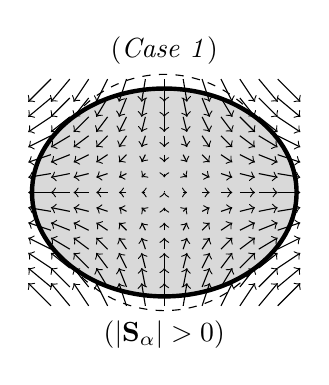
\begin{tikzpicture}[ultra thick,scale=0.6]
        \def\nRows{6}
        \def\nCols{6}
        \draw[dashed,thin] (0,0)circle(2.5);
        \draw[fill=gray!30] (0,0)ellipse(2.8 and 2.2);
        \foreach \x in {-\nRows,...,\nRows} {
            \foreach \y in {-\nCols,...,\nCols} {
                \pgfmathsetmacro\distance{veclen(\x*0.4, \y*0.4)};
                \pgfmathparse{\distance < 2.45 ? "blue" : "white"}
                \edef\colour{\pgfmathresult};
                \ifthenelse{\equal{\colour}{blue}}{                    
                    \draw[thin,->](\x*0.4,\y*0.4)--++(0.08*\x,-0.08*\y);
                }
            }
        }
        \node (txt) at (0,3){(\textit{Case 1})};
        \node (txt) at (0,-3){($|\textbf{S}_\alpha| > 0$)};
    \end{tikzpicture}
     \hfill
    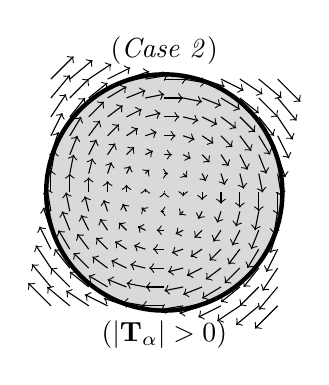
\begin{tikzpicture}[ultra thick,scale=0.6]
        \def\nRows{6}
        \def\nCols{6}
        \draw[fill=gray!30] (0,0)circle(2.5);
        \foreach \x in {-\nRows,...,\nRows} {
            \foreach \y in {-\nCols,...,\nCols} {
                \pgfmathsetmacro\distance{veclen(\x*0.4, \y*0.4)};
                \pgfmathparse{\distance < 2.5 ? "blue" : "white"}
                \edef\colour{\pgfmathresult};
                \ifthenelse{\equal{\colour}{blue}}{                    
                    \draw[thin,->](\x*0.4,\y*0.4)--++(0.08*\y,-0.08*\x);
                }
            }
        }
        \node (txt) at (0,3){(\textit{Case 2})};
        \node (txt) at (0,-3){($|\textbf{T}_\alpha| > 0$)};
    \end{tikzpicture}
    \hfill
    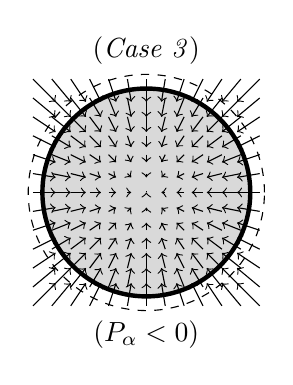
\begin{tikzpicture}[ultra thick,scale=0.6]
        \def\nRows{6}
        \def\nCols{6}
        \draw[dashed,thin] (0,0)circle(2.5);
        \draw[fill=gray!30] (0,0)circle(2.2);
        \foreach \x in {-\nRows,...,\nRows} {
            \foreach \y in {-\nCols,...,\nCols} {
                \pgfmathsetmacro\distance{veclen(\x*0.4, \y*0.4)};
                \pgfmathparse{\distance < 2.3 ? "blue" : "white"}
                \edef\colour{\pgfmathresult};
                \ifthenelse{\equal{\colour}{blue}}{                    
                    \draw[thin,->](\x*0.4,\y*0.4)--++(-0.08*\x,-0.08*\y);
                }
            }
        }
        \node (txt) at (0,3){(\textit{Case 3})};
        \node (txt) at (0,-3){($P_\alpha < 0$)};
    \end{tikzpicture}
    \hfill
    \caption{Graphical representation of the inner kinematics   of an arbitrary particle under three scenarios. 
        The arrows represent the velocity field inside the particle, $\textbf{w}_d^0$, with the corresponding value of the moment of momentum tensor indicated below. 
        The operator $|\ldots|$ refers to the norm of the tensors. 
        According to the inner velocity field:
        (\textit{Case 1}) The particle experiences a mean deformation, resulting in non-zero stretching of momentum along the principal axis of deformation;
        (\textit{Case 2}) The particle is rotating, leading to a non-zero angular momentum vector in the direction of rotation;
        (\textit{Case 3}) The particle undergoes compression, resulting in a negative trace of the moment of momentum.
    }
    \label{eq:scheme}
\end{figure}
Injecting, $f_d^0 = \rho_d$ in the second-order moment equation (derived in \ref{ap:Moments_equations}) we obtain,
%\JL{pq lequation du second moment de la masse ne fait pas intervenir la trace du premier moment de la qdm - cela semble incoherent ?}
\begin{equation}
    \ddt {\textbf{M}_\alpha}=2(\textbf{S}_\alpha+P_\alpha\bm\delta),
    \label{eq:dt_M_alpha}
\end{equation}
which is the second-order moment of mass conservation equation assuming that the fluid within the drop is divergence free. 
From \ref{eq:dt_M_alpha} we deduce that the evolution of the distribution of mass of a particle is solely determined by the  of momentum $\textbf{S}_\alpha$ and $P_\alpha$. 
This indicates that angular momentum does not influence the evolution of the second moment of mass, a consequence of the symmetry of the tensor $\textbf{M}_\alpha$, which must be preserved after differentiation with respect to time.
However, this does not imply that the particle angular velocity ($\bm\omega_\alpha$) does not appear in this equation. 
For instance, in the case of rigid body motion where $\textbf{w}_d^0 = \bm\omega_\alpha \times \textbf{r}$, we obtain the relation  $2(\textbf{S}_\alpha)_{ij} = \epsilon_{iab} (\bm\omega_\alpha)_a (\textbf{M}_\alpha)_{bj}+ 
\epsilon_{jab} (\bm\omega_\alpha)_a (\textbf{M}_\alpha)_{bi}  $. 

Now that we have described the kinematics   of the particle shape, let us proceed to derive an equation for the moment of momentum.
This equation is derived by injecting $\textbf{Q}_\alpha^{(1)} = \textbf{P}_\alpha$ in \ref{eq:dt_Q_alpha_tot}, it reads, 
\begin{equation}
    \ddt {\textbf{P}_\alpha}
    - \intO{ \rho_d  \textbf{w}_d^0 \textbf{w}_d^0 }
    = 
    - \intO{\bm{\sigma}_d^0}
    - \intS{ 
        \gamma (\bm\delta - \textbf{nn})
    }
    + \intS{ \textbf{r}\bm{\sigma}_f^0\cdot \textbf{n}}.
    \label{eq:dt_P_alpha}
\end{equation}
In the following sections the normal vector noted \textbf{n} always refer to $\textbf{n}_d$. 
The conservation equation of the angular momentum $\bm{\mu}_\alpha$ is obtained by taking the double contracted product of \ref{eq:dt_P_alpha} with $\bm\epsilon$, which directly gives
\begin{equation}
    \ddt\bm{\mu}_\alpha
    =  
    % \textbf{t}_\alpha.
    \intS{ \textbf{r} \times \bm{\sigma}_f^0\cdot \textbf{n} }
    \label{eq:dt_mu_alpha}
\end{equation}
Note that every term on the right-hand side of \ref{eq:dt_P_alpha} vanished due to their symmetric nature apart from the skew-symmetric part of the hydrodynamic stress, which is the hydrodynamic torque applied on the particle $\alpha$.
In particular, the surface tension terms do not appear in the angular momentum balance since the tensor $\bm\delta-\textbf{nn}$ is symmetric, which is consistent with the findings of \citet{hesla1993note}. 
As a consequence, the surface tension does not affect the angular momentum regardless of the particle shape. 
%In the literature, it is common to include the torque due to inter-particular interactions in the angular momentum balance, as is done in \citet{jackson1997locally} and \citet{zhang1997momentum}.
%In our case note that $\bm{\sigma}_f^0$ contains short-range hydrodynamic interaction forces. 

Taking the symmetric part of \ref{eq:dt_P_alpha}, and substrating the trace yields, 
\begin{align}
    &\ddt {\textbf{S}_\alpha}
    - \rho_d\intO{\left(\textbf{w}_d^0 \textbf{w}_d^0 -\frac{1}{3} (\textbf{w}_d^0 \cdot  \textbf{w}_d^0)\bm\delta\right)}
    = \nonumber \\
    &- 2\mu_d\intO{\textbf{e}_d^0}
    -  \intS{ \gamma
        \left( \frac{1}{3}\bm\delta - \textbf{nn} \right)
    }
    + \frac{1}{2}\intS{\left(\textbf{r}\bm\sigma_f^0+\bm\sigma_f^0\textbf{r}-\frac{2}{3}(\bm\sigma_f^0 \cdot \textbf{r})\bm\delta \right)\cdot \textbf{n}},
    \label{eq:dt_S_alpha}
\end{align}
%internal velocity kinetic energy. %$\intO{\rho_d\textbf{w}_d^0\textbf{w}_d^0 }$.
%On the left-hand side of \ref{eq:dt_S_alpha} we identify two inertial terms, i.e. the derivative of $\textbf{S}_\alpha$ and the stress induced by the product of internal velocity within the drop.
%The inertia of the particle is then balanced by the terms on the right-hand side of the equation, namely: 
%the volumic integral of the particle viscous stress; 
%the surface integral of the surface tension stress ; 
%and the first moment of the hydrodynamic stress tensor.
%A discussion regarding the physical implications of this equation is provided below. 
where we have introduced the rate of strain tensor for phase \( k \), defined as \( \mathbf{e}_k^0 = \frac{1}{2} (\grad \mathbf{u}_k^0 + ^\dagger \grad \mathbf{u}_k^0) \). 
Here $^\dagger$ represents the transpose operator. 
On the left-hand side of Equation~\ref{eq:dt_S_alpha}, two inertial contributions can be identified: the time derivative of $\mathbf{S}_\alpha$, and the stress arising from the product of internal velocity field within the droplet. 
These inertial effects are counterbalanced by the terms appearing on the right-hand side of the equation, which include: the volume integral of the particle viscous stress; the surface tension moment; and the first moment of the hydrodynamic force.
%\JL{a finaliser}
While surface tension effects do not influence the linear or angular momentum equations directly, they do impact the moment of momentum $\textbf{P}_\alpha$, specifically its symmetric part $\textbf{S}_\alpha$.
Consequently, surface tension influences the hydrodynamic behavior of a particle exclusively through its effect on $\textbf{S}_\alpha$, which is related to the shape of a particle represented by $\textbf{M}_\alpha$, via \ref{eq:dt_M_alpha}.
%Whether it is solid or fluid particles \ref{eq:dt_S_alpha} becomes particularly relevant for expressing the averaged stress within an inertial suspension in terms of Lagrangian properties, as discussed in the next chapter. 
%\JL{enlever la trace}
%Taking the symmetric part of \ref{eq:dt_P_alpha}, and making use of \ref{eq:dt_M_alpha}, yields a dynamical balance equation for $\textbf{M}_\alpha$, namely
Inserting \ref{eq:dt_S_alpha} in  \ref{eq:dt_M_alpha} yields,
%\JL{enlever la trace et reecrire la partie ci-dessous + donner la definition de $e_d$ qui n'est pas de defini avant.}
\begin{align}    
    &\frac{1}{2}\frac{d^2 (\textbf{M}_\alpha-\frac{1}{3}(\textbf{M}:\bm\delta)\bm\delta)}{dt^2}
    =  \rho_d\intO{\left(\textbf{w}_d^0 \textbf{w}_d^0 -\frac{1}{3} (\textbf{w}_d^0 \cdot  \textbf{w}_d^0)\right)}
    - 2\mu_d\intO{\textbf{e}_d^0} \nonumber\\
    &- \intS{\gamma  
        \left( \frac{1}{3}\bm\delta - \textbf{nn} \right)
    }
    + \frac{1}{2}\intS{\left(\textbf{r}\bm\sigma_f^0+\bm\sigma_f^0\textbf{r}-\frac{2}{3}(\bm\sigma_f^0 \cdot \textbf{r})\bm\delta \right)\cdot \textbf{n}}.
    \label{eq:dt2_M_alpha}
\end{align}
%On the left-hand side of \ref{eq:dt_S_alpha}, we recover the symmetric part of the inertial contributions. 
%In opposition to \ref{eq:dt_P_alpha} we could substitute the term $\ddt (\textbf{P}_\alpha+\textbf{P}_\alpha^\dagger)$ initially present in the equation by $\ddt^2 \textbf{M}_\alpha$ using \ref{eq:dt_M_alpha}. 
%\ref{eq:dt2_M_alpha} is a second-order partial differential equation for the second order mass moment characterizing the droplet shape.
%In other words, \ref{eq:dt2_M_alpha} must be interpreted as an equation for the shape of the particle, represented by the tensor $\textbf{M}_\alpha$. 
%Thus, on the right-hand side of \ref{eq:dt_S_alpha}, we identify the terms which favors deformation, including the inertia of the velocity field within the droplet as well as the traceless part of the first moment and the terms wwohc resis deformation incluidng the viscous resistance within the droplet and the surface tension.
\ref{eq:dt2_M_alpha} is a second-order differential equation governing the second-order mass moment that characterizes the droplet shape. 
In other words, it should be interpreted as an equation describing the droplet shape, represented by the traceless part of the tensor $\textbf{M}_\alpha$.
Accordingly, the right-hand side of \ref{eq:dt2_M_alpha} contains terms that promote deformation-such as the product of the internal velocity field and the traceless component of the first moment as well as terms that oppose deformation, including droplet internal viscous resistance and surface tension.
%One might also recognize that \ref{eq:dt2_M_alpha} is in fact an extension of \citet{batchelor1970stress} result, but with the consideration of the inertia of the particle.
\ref{eq:dt2_M_alpha} is particularly useful to compute the unknown internal stress within solid particles, in terms of surface integral, i.e. the first moment of the hydrodynamic force.
This relation plays a key role in expressing the bulk stress of a suspension and ultimately leads to the effective viscosity, once a closed-form expression for the average first moment is obtained \citep{batchelor1970stress}. 
In the inertial regime, and for solid particles, the tensors $\textbf{M}_\alpha$ and the internal velocity field $\textbf{w}_d^0$ are fully prescribed by the particle kinematics. 
As a result, in \ref{eq:dt2_M_alpha}, $\textbf{M}_\alpha$ and $\textbf{w}_d^0$ appear not as unknowns but rather as known source terms.
For spherical particles specifically, the inertial correction to the first force moment has been derived by \citet{hwang1989modeling} and  \citet{lhuillier1996contribution}.
%For the specific case of spherical particles \citet{hwang1989,lhuillier1996contribution} have derived this inertial correction.
%This relation is used to express the bulk stress of a suspension.
%It eventually leads to the computation of the famous Einstein equivalent viscosity, upon having a closed expression for the average of the first moment \citep{guazzelli2011}. 
%In the inertial case and for solid particle, the tensors $\textbf{M}_\alpha$ and the inner velocity field $\textbf{w}_d^0$ are fully determined by the particle kinematic, indicating that $\textbf{M}_\alpha$ and $\textbf{w}_d^0$ can be used in \ref{eq:dt_S_alpha} not as unknowns but as source terms. 
%Consequently, for solid particles, \ref{eq:dt_S_alpha} must be interpreted as a generalized equation for the undefined stress $\bm\sigma_d^0$ integrated on the volume of the particles.

%Note that if intead we had considered spherical particles composed of compressible fluid \ref{eq:dt2_M_alpha} transforms into the Rayleigh-Lamb-Plesset equation as demonstrated in \citep{danielcours}.


%In our case, only the external contribution $\intS{\textbf{r}\bm\sigma_f^0\cdot \textbf{n}}$ is responsible for the generation of angular momentum, see \ref{eq:dt_mu_alpha}.
%Taking the symmetric part of this tensor ultimately removes this contribution. 

%\begin{equation}
%    \intO{\bm{\sigma}_d^0}
%    + \intS{\gamma(\bm\delta - \textbf{nn})}
%    = \frac{1}{2}\intS{(\textbf{r}\bm\sigma_f^0+\bm\sigma_f^0\textbf{r})\cdot \textbf{n}},
%    \label{eq:Batchelor}
%\end{equation}

%In \ref{ap:Moments_equations} we show how to derive the higher-order moment of momentum equations, which can also be viewed as formulas for the higher moments of the internal particle stress distribution. 
%It is interesting to mention that in a recent study of \citet{dolata2021faxen} and \citet{zhou2020lamb} they make use of the first two moments of momentum equations hidden into another but equivalent form, valid in the Stokes flow regime. 








\subsection{Averaged momentum and mass conservation equations}



Let us now focus on the averaged momentum equation of the continuous phase. 
By applying \eqref{eq:dt_f_k} with $f_k = \rho_f$ and $\rho_f\textbf{u}_f$ we obtain the mass and momentum equation for the continuous phase under the two fluid formulation, 
\begin{align}
    (\pddt + \textbf{u}_f\cdot \grad)\textbf{u}_f&=-\phi_f \div \textbf{u}_f
    \label{eq:mass_init}\\
    \phi_f \rho_f(\pddt + \textbf{u}_f  \cdot \grad) \textbf{u}_f
    % +  \div \avg{\chi_f\rho_f \textbf{u}_f'\textbf{u}_f'}
    &= 
    \div [\phi_f \bm\sigma_f-  \avg{\chi_f\rho_f \textbf{u}_f'\textbf{u}_f'}]
    + \phi_f \rho_f \textbf{g}
    - \avg{\delta_\Gamma \bm\sigma_f\cdot \textbf{n}}.
    \label{eq:two_fluid_momentum_init}
\end{align} 
To obtain the hybrid formulation one can expand the final term on the right-hand side of \ref{eq:two_fluid_momentum_init} using the Taylor expansion provided in \ref{eq:f_exp}.  
However, before doing so, it is important to examine the term \( \phi_f \bm\sigma_f \), as it contains a non-closed contribution originating from the averaging of the strain rate tensor. %a contribution from the dispersed phase. 
Properly identifying and isolating this contribution is a necessary step prior to performing the Taylor expansion.
%Moreover, there

%one may use \ref{eq:f_exp} to taylor expand the last term on the right-hand side of \ref{eq:two_fluid_momentum_init}. 
%However, it is first important to discuss the form of the term $\phi_f\bm\sigma_f$ since a dispersed phase term, is hidden into it, hence it is important to identify this term before carrying out the Taylor expansion. 

%\subsection{Mean stress formulation and momentum transfer decomposition}
%\JL{bien expliquer quand et comment apparaissent les distinctions sur le choix de la contrainte moyenne. en particulier voir en dessous}

We begin by noting that $\phi_f\bm\sigma_f$ can be expressed in terms of the averaged fluid pressure $p_f$, and continuous phase averaged velocity ($\textbf{u}_f$), or bulk-averaged velocity ($\textbf{u} = \phi_f \textbf{u}_f + \phi_d \textbf{u}_d$).
Expressing $\bm\sigma_f$ as a function of $\textbf{u}_f$ instead of $\textbf{u}$ (or vice versa) leads to two distinct forms of the momentum equation, each associated with different formulations of the closure terms. 
We also review several alternative choices found in the literature (see also \citet{jackson2000, pahtz2025general} for an overview focused on solid particles), emphasizing that while all these formulations are mathematically equivalent, they give rise to different closure problems. 
We argue that one particular formulation is probably the most suitable, especially in light of the closure terms available in the literature for non-dilute flows.%especially in the context of existing closure models for non-dilute flows.
%Choosing to express $\bm\sigma_f$ as a function $\textbf{u}_f$ rather than $\textbf{u}$ and vice versa, results in two distinct forms of the momentum equation and two distinct formulations of the closure terms. 
%We also discuss the various other choice available on the literature (see also \citet{jackson2000,pathz2025} for a review for solid particles) explaining that there is all choice are perfectly equivalent but leads to a different closure problems.
%Our belief his that there is one formulation which is the most appropriate with respect to of the closure terms available in the litterature for non-dilute flow.
%Although this topic has been already discussed in the context of solid particles  we propose here to expose both formulations and discuss which of the two equivalent (but different) formulations is the most suited for multiphase flow modeling. 

%Because we believe this topic has not been discussed much for non-solid particles in the literature, we propose here to expose both formulations and discuss which of the two equivalent (but different) formulation is the most suited for multiphase flow modeling. 
%Because we believe this topic has not been discussed much in the literature for non-solid particles, 

First we introduce what we refer to as the \textit{mean Newtonian stress}, based either on the continuous phase averaged velocity $\textbf{u}_f$ or on the bulk velocity \textbf{u}, namely,
\begin{align}
    \bm\Sigma_f 
    &
    = -p_f \bm\delta + 2\mu_f \textbf{E}_f    
    %= -p_f \bm\delta + \mu_f [\grad \textbf{u}_f + (\grad \textbf{u}_f)^{\dagger}], 
    \label{eq:Sigma_f_average}
    \\
    \bm\Sigma &
    = -p_f\bm\delta + 2 \mu_f \textbf{E}
    %= -p_f \bm\delta + \mu_f [\grad \textbf{u} + (\grad \textbf{u})^{\dagger}],
    \label{eq:Sigma_average}
\end{align}
where $\textbf{E}_f = [\grad \textbf{u}_f + (\grad \textbf{u}_f)^{\dagger}]/2$ and $\textbf{E} =[\grad \textbf{u} + (\grad \textbf{u})^{\dagger}]/2$ represent the \textit{mean strain rate} tensor based either on $\textbf{u}_f$ or on \textbf{u}. 
Additionally the ensemble averaged stress $\phi_f \bm\sigma_f$ may be written as 
\begin{equation}
    \phi_f \bm\sigma_f = - \phi _f p_f \bm\delta + 2 \mu_ f \phi_f \textbf{e}_f
    \label{eq:sigma_average}
\end{equation}
where $\phi _f \textbf{e}_f = \avg{\chi _f \textbf{e}_f^0}$. 
%Moreover by definition the bulk stress tensor reads $\textbf{E} = \phi _f\textbf{e}_f + \phi_d \textbf{e}_d$.
Inserting \ref{eq:Sigma_f_average} and \ref{eq:Sigma_average} in  \ref{eq:sigma_average} yields
%Using the constitutive law of Newtonian fluids we find, 
\begin{align}
    \phi_f \bm\sigma_f 
    &=
    % - \phi_f p_f \bm\delta
    % + \phi_f \mu_f [\grad \textbf{u}_f  + (\grad \textbf{u}_f)^\dagger]
    % - \mu_f \avg{\delta_\Gamma( \textbf{u}_f'  \textbf{n} +  \textbf{n} \textbf{u}_f' )}
    % =
    \phi_f \bm\Sigma_f
    - \mu_f \avg{\delta_\Gamma( \textbf{u}_f'  \textbf{n} +  \textbf{n} \textbf{u}_f' )}
    \label{eq:stress_closure}\\
    \phi_f \bm\sigma_f 
    &=
    % - \phi_f p_f \bm\delta
    % + \mu_f [\grad \textbf{u}  + (\grad \textbf{u})^\dagger]
    % - 2\mu_f \phi_d \textbf{e}_d
    % =
    \phi_f \bm\Sigma
    - \avg{2\mu_f \chi_d \textbf{e}_d^*}
    \label{eq:stress_closure1}
\end{align}
where we have used the relations 
\begin{equation}
    \avg{\chi_f \grad \textbf{u}_f^0}
    = 
    \phi_f \grad  \textbf{u}_f
    + \avg{\delta_\Gamma \textbf{n}_f \textbf{u}_f'}
    \label{eq:first_rel}
\end{equation}
and
\begin{equation}
    %\avg{\chi_f \textbf{e}_f^0}
%    = 
%    \avg{\textbf{e}^0}
%    - \avg{\chi_d \textbf{e}_d^0}
\phi _f\textbf{e}_f
%    = 
%    \textbf{E}
%    - \avg{\chi_d \textbf{e}_d^0}
    = 
    \phi_f \textbf{E}
    - \avg{\chi_d \textbf{e}_d^*},
    \label{eq:sec_rel}
\end{equation}
to derive \ref{eq:stress_closure,eq:stress_closure1}, respectively. 
 %in most practical situations of interest.
%Note that \ref{eq:first_rel} remains true in the presence of non zero interfacial rate of strain, while \ref{eq:sec_rel} requires the condition that the bulk rate of strain reads $\textbf{E} = \phi _f\textbf{e}_f + \phi_d \textbf{e}_d$ \textit{i.e.} that there is no shear stress at the interface of the droplets, so that $\avg{\delta_\Gamma \textbf{e}_\Gamma^0}= 0$, which is true in most of the practical cases of interest. 
In \ref{eq:stress_closure1} we have introduced $\textbf{e}_d^* = \textbf{e}_d^0 - \textbf{E} = \grad (\textbf{u}_d^0-\textbf{u})+\grad (\textbf{u}_d^0-\textbf{u})^\dagger$ which is the droplet internal shear rate relative to the `bulk' shear rate \textbf{E}.
%While $\textbf{u}_f' = \textbf{u}_f^0 - \textbf{u}_f$ in \ref{eq:stress_closure}. 
It is worth noting that \ref{eq:first_rel} remains valid even when the interfacial rate of strain is nonzero. 
In contrast, \ref{eq:sec_rel} holds under the assumption that the bulk rate of strain satisfies $\textbf{E} = \phi_f \textbf{e}_f + \phi_d \textbf{e}_d$, \textit{i.e.} that $\avg{\delta_\Gamma \textbf{e}_\Gamma^0} = 0$. 
This condition is supposed to be met here because we did not consider interfacial viscosity\citep{nadim1996concise}.
%Before presenting the hybrid form of the continuous phase momentum equation, it is interesting to expose the classic two-fluid formulation using the stress formulation given by \ref{eq:stress_closure} in the first place. 
%Before introducing the hybrid form of the continuous phase momentum equation, it is useful to first present the classical two-fluid formulation, employing the stress formulation \ref{eq:stress_closure}.
The averaged momentum equation  employing the stress formulation \ref{eq:stress_closure} read, 
\begin{align}
    % (\pddt + \textbf{u}_f\cdot \grad)\textbf{u}_f&=-\phi_f \div \textbf{u}_f\\
    \phi_f \rho_f(\pddt + \textbf{u}_f  \cdot \grad) \textbf{u}_f
    % +  \div \avg{\chi_f\rho_f \textbf{u}_f'\textbf{u}_f'}
    &= \phi_f 
    \left(\div \bm{\Sigma}_f
    + \rho_f \textbf{g}\right)
    - \div 
    [\avg{\chi_f\rho_f \textbf{u}_f'\textbf{u}_f'}
    +\avg{\delta_\Gamma \mu_f( \textbf{u}_f'  \textbf{n} +  \textbf{n} \textbf{u}_f')}]
    - \avg{\delta_\Gamma \bm\sigma_f^{(1)}\cdot \textbf{n}},
    \label{eq:two_fluid_momentum}
\end{align}
where, $\bm\sigma_f^{(1)}=\bm\sigma_f^0 - \bm\Sigma_f$ which also reads %is the Newtonian stress evaluated at a point on an interface relative to the mean stress $\bm\Sigma_f$. 
\begin{equation}
\bm\sigma_f^{(1)} = -p_f'\bm\delta
+ \mu_f [
    \grad \textbf{u}_f'
    + ^\dagger \grad \textbf{u}_f']
    \label{eq:disturbance_stress1}
\end{equation} 
Likewise, using \ref{eq:stress_closure1} one may also derive another form of the momentum equation, namely,
\begin{equation}
    \phi_f \rho_f(\pddt + \textbf{u}_f  \cdot \grad) \textbf{u}_f
    % +  \div \avg{\chi_f\rho_f \textbf{u}_f'\textbf{u}_f'}
    = \phi_f 
    \left(\div \bm{\Sigma}
    + \rho_f \textbf{g}\right)
    - \div 
    [\avg{\chi_f\rho_f \textbf{u}_f'\textbf{u}_f'} + \avg{2\mu_f \chi_d \textbf{e}_d^*}]
    - \avg{\delta_\Gamma \bm\sigma_f^{(2)}\cdot \textbf{n}},
    \label{eq:two_fluid_momentum2}
\end{equation} 
where $\bm\sigma_f^{(2)}=\bm\sigma_f^0 - \bm\Sigma$. 
%This stress tensor corresponds to the Newtonian stress (relative to the mean pressure and velocity field) typically available in numerical or theoretical studies. 
It can be also expressed as, 
%Clearly, subtracting by $\bm\Sigma_f$ to the local stress at the interface leads to the expression 
\begin{equation}
    \bm\sigma_f^{(2)} 
    =
    -p_f'\bm\delta
    + \mu_f [
        \grad \textbf{u}_f^*
        + ^\dagger \grad \textbf{u}_f^*
    ]
    \label{eq:disturbance_stress2}
\end{equation}
where $\textbf{u}_f^*= \textbf{u}_f^0 - \textbf{u}$.
%which corresponds to the Newtonian stress at the surface of the droplets (relative to the mean pressure and velocity field) typically available in numerical or theoretical studies.
%Likewise, substituting the mean stress with $\bm\Sigma$ in \ref{eq:disturbance_stress} one obtain the same formula except than $\textbf{u}_f'\to \textbf{u}_f^0 - \textbf{u}$. 
%Hence, 
In both cases (\ref{eq:two_fluid_momentum} and \ref{eq:two_fluid_momentum2}) one has to compute the local stress relative to the averaged continuous phase motion or bulk phase motion. 
% Note that because $\div \textbf{u} = 0$ it may be more convenient to  
%Note the differences between the last term of formulation \ref{eq:stress_closure} and \ref{eq:stress_closure1}, is equal to, $\phi_f (\div \bm\Sigma_f - \div\bm\Sigma)$
%Hence, the transition from one formulation to the other is straightforward, it just requires adding or subtracting $\phi_f (\div \bm\Sigma_f - \div\bm\Sigma)$. 
%However it is worth noting the physicsical meaning og this term which also reads,
Note the difference between the last terms in formulations \ref{eq:stress_closure} and \ref{eq:stress_closure1}, which is given by $\phi_f \div (\bm\Sigma_f -\bm\Sigma)$.
The transition from one formulation to the other is straightforward and only requires the addition or subtraction of this term. 
However, it is important to recognize its physical significance.
This difference can be expressed explicitly as,
\begin{equation}
    \phi_f \div(\bm\Sigma_f - \bm\Sigma) = \mu_f \phi_f \div \left[\grad (\phi_d (\textbf{u}_f - \textbf{u}_d)) + \grad (\phi_d (\textbf{u}_f - \textbf{u}_d))^\dagger \right]
    \label{eq:diff_sigma1}
\end{equation}
where the decomposition 
\begin{equation}
\textbf{u} = \phi_f \textbf{u}_f + \phi_d \textbf{u}_d,
\label{eq:u_mean} 
\end{equation}
has been used in the derivation.
\ref{eq:diff_sigma1} reveals that the difference between the two formulations introduces a non-Newtonian stress term.
This non-Newtonian stress shares similarities with the second-order force moment closure \citep{jackson1997locally,zhang1997momentum}, and it is typically related to intrinsic convection in sedimentation processes \citep{lhuillier2022}.
Therefore, when addressing the closure problem, it is essential to treat each stress formulation carefully, as the inclusion or exclusion of this additional term can significantly impact the resulting model.
%Then, when considering the colsure problem one has to be carefull to properly consider each formulation of the stress differently as both formulation will resulst in adding or removing this term.
%between \ref{eq:def_sigma_eff_f} and \ref{eq:def_sigma_eff_f2}  plus the differences between the corresponding drag force terms, is exactly equal to, $\phi_f (\div \bm\Sigma_f - \div\bm\Sigma)$.
%\JL{il faut que tu m'expliques : quand je soustrais les forces j'obtiens $\phi (\div \bm\Sigma_f - \div\bm\Sigma)$. OK on soustrait juste le RHS par ailleurs je pense qu'il faut detailler cela, c'est un point important.}
%\JL{en particulier $\div \bm\Sigma_f - \div\bm\Sigma = \div \nabla u_f - u \propto u_r$  a expliciter en montrant le developpment limite}





%Even though, both stress decomposition and momentum formulations proposed here are equivalent, each formulation have advantages and drawback which we discuss below.  
Although the stress decomposition and momentum formulations proposed herein are mathematically equivalent, each presents distinct advantages and limitations, which we examine in detail below.
%Now let us discuss on the choic between $\bm\Sigma$ and $\bm\Sigma_f$. 
%At first sight, using \ref{eq:dt_uf} with the effective stress given by \ref{eq:def_sigma_eff_f}, seems more practical because we are solving for the field $\textbf{u}_f$ hence avoiding the need of \ref{eq:velocity_conservation}. 
First, we may observe that a simplification arises for \ref{eq:stress_closure1} in the case of solid particles, for which $\textbf{e}_d^0 = 0$.
As a result $\phi _f \bm \sigma _f = - \phi _f p_f \bm\delta + 2 \mu_ f \textbf{E}$ \citep{joseph1990ensemble,jackson2000}. %and $\avg{\chi_d \textbf{e}_d^*} = -\phi\bm\Sigma$. \JL{a montrer}
Owing to this simplification, the formulation based on $\bm\Sigma$ and the associated closure relation \eqref{eq:stress_closure1} makes it a good candidate to be used in practice for solid particles. %is frequently adopted in the literature \citep{jackson2000}, despite requiring the inclusion of the additional momentum conservation equation.
Second, employing \ref{eq:two_fluid_momentum} with \ref{eq:disturbance_stress1} may appear more convenient as the governing equations are directly formulated in terms of the fluid velocity field $\textbf{u}_f$, thereby circumventing the need to explicitly include an expansion for the bulk fluid velocity. %the following equation
%Because $\textbf{u}$ may be required by \ref{eq:stress_closure1}, one also need to solve the equation, 
%\eqref{eq:velocity_conservation}.
%On the other hand we note that for solid particles $\textbf{e}_d^0 = 0$ and $\avg{\chi_d \textbf{e}_d'} = -\bm\Sigma\phi$, because of this great simplification \ref{eq:stress_closure1} is often used \citep{jackson2000} even if it requires adding \ref{eq:velocity_conservation} in the system of equation.  
%\JL{Je comprends l'interet de cette simplification, mais il faur toujours avoir une exression pr $\textbf{E}$ donc pour $\textbf{u}$}
Third, there exists a conceptual reason for preferring the bulk stress $\bm\Sigma$ when deriving closure relations for non-dilute suspensions.  %involving the fluctuating stress $\bm\sigma_f'$. 
Specifically, because $\bm\sigma_f^{(2)}$ depends on the disturbance velocity $\textbf{u}_f^* = \textbf{u}_f^0 - \textbf{u}$, the averaged velocity $\textbf{u}$ naturally serves as the "far-field" or "undisturbed" velocity boundary condition in the conditionally averaged Navier-Stokes equations \citep{hinch1977averaged,fintzi2025}. %(as also emphasized in the context of this PhD study).
%But there is another reason for using the `bulk stress' $\bm\Sigma$ as a reference stress to compute the closure terms involving $\bm\sigma_f'$. 
%Indeed, since $\bm\sigma_f'$ requires $\textbf{u}_f' = \textbf{u}_f^0 - \textbf{u}$, then \textbf{u} becomes the `far field' or `undisturbed' velocity boundary condition far from the test particle in the conditionally averaged Navier-Stokes equations \tb{(+my phd)}.
%On another hand, one may note that all the available theoretical solutions considering the disturbance field of a particle embedded in a pure solvent or in an effective medium (which represents other particles' contribution) use a divergence free `background flow' as limiting condition \citep{kim1985modelling,hinch1977averaged}.
%Since $\div \textbf{u} =0$ we deduce that the velocity field used in most (if not all) theoretical problems correspond to \textbf{u}. 
%Therefore, the disturbance  stress computed in these problems is $\bm\sigma_f'= \bm\sigma_f^0 - \bm\Sigma$. 
Notably, most (if not all) existing theoretical solutions addressing the disturbance field generated by a particle embedded in a Newtonian solvent or in an effective medium - representing other particles contribution - use a divergence-free background velocity field as limiting boundary condition \citep{hinch1977averaged, kim1985modelling}. 
Since $\div \textbf{u} = 0$, it follows that the velocity field used in these theoretical study corresponds to $\textbf{u}$. 
Consequently, the disturbance stress derived in those studies is $\bm\sigma_f^{(2)} = \bm\sigma_f^0 - \bm\Sigma$.
In opposition, the stress decomposition based on $\bm\Sigma_f$, involves the fields $\textbf{u}_f$ which is not divergence free. 
Hence, this `far field' or `undisturbed' velocity boundary condition far from the test particle does not correspond to the usual boundary condition assumed in most of the theoretical problems. 
%In conclusion, it is important to note that \textbf{u} corresponds exactly to the `background velocity' fields used in most of the theoretical derivations.
%Hence, the resulting closure terms (drag forces, stresslet and higher moments) derived in these studies refer to the closures expressed in terms of $\bm\sigma_f^0 - \bm\Sigma$.
%In all case one can always express $\bm\Sigma_f$ in terms of $\bm\Sigma$ hence which formulation to use is not a fatality. 
%However, one must always be careful when asserting that a given formulation of the drag force, for example, is exactly equivalent to a closure term found in the literature, as there are multiple possible formulations  (either based on $\bm\Sigma_f$, $\bm\Sigma$, $\bm\sigma_f$ or even  $p_f \bm\delta$). 
%Note that the choices between $\bm\Sigma_f$ and $\bm\Sigma$ only matter if one consider a closure problem, in which $\phi \textbf{u}_f \neq \phi \textbf{u}$, hence accurate at $O(\phi^2)$ at least (such as in \citet{hinch1977averaged,kim1985modelling}). 
In conclusion, it is important to recognize that the vector field \(\textbf{u}\) corresponds precisely to the 'background velocity' typically employed in theoretical derivations. 
Consequently, the closure terms obtained in such analyses -such as the hydrodynamic forces, the stresslet, and higher-order moments- are formulated in terms of the difference \(\bm\sigma_f^0 - \bm\Sigma\).
Of course, it is always possible to express \(\bm\Sigma_f\) in terms of \(\bm\Sigma\) (see \ref{eq:diff_sigma1}), meaning that the choice of formulation remains free. 
Nevertheless, we must be cautious when claiming that a specific expression of, for example, the Faxen contribution to the force is exactly equivalent to a closure term reported in the literature especially for non-dilute suspension. 
%Multiple valid formulations exist, involving \(\bm\Sigma_f\), \(\bm\Sigma\), \(\bm\sigma_f\), or even the pressure tensor \(p_f \bm\delta\).
% It should also be noted that the distinction between $\bm\sigma_f^{(1)}$ and $\bm\sigma_f^{(2)}$ becomes relevant only in the context of closure problems accurate at \(O(\phi^2)\) or more\footnote{Indeed, because $\textbf{u} \phi = \textbf{u}_f\phi +O(\phi^2)$ the distinction between bulk or continuous phase averaged velocity field becomes irrelevant in the closure problem. }. 
% \JL{pas compris cette derniere phrase que je pense il faut enlever : on montre que la distinction joue deja pour le second moment des forces en regime dilue non ?}

% \JL{je n'ai pas compris le paragraphe suivant - je ne sais pas si il est necessaire desormais vu l'organisation actuelle ou on fait le developement en serie de Taylor plus tard}
% One can remark the similarities between the surface exchange terms expansion, and the multipole expansion used in microhydrodynamic that characterize the disturbance field caused by a body immersed in a stokes flow \citet{pozrikidis1992boundary,kim2013microhydrodynamics}. 
% Moreover, one can wonder which of the formulation, \ref{eq:def_sigma_eff_f2} or \ref{eq:def_sigma_eff_f}, contains what is called the `Stresslet' and the higher moments of force given by the multipole expansion used in microhydrodynamic ? \citep{pozrikidis1992boundary,kim2013microhydrodynamics}\footnote{Note that the first term in this expansion is the same whether we use \ref{eq:def_sigma_eff_f2} or \ref{eq:def_sigma_eff_f}}.   
% These moments are usually defined as the `extra stress above the value of the fluid law'\citep{hinch1977averaged}.
% Because we are not studying the `bulk' momentum equation this definition does not directly apply in our context. 
% However, note that \ref{eq:stress_closure1} involves the bulk velocity \textbf{u} which must be used in the bulk stress momentum equation.
% Hence, we can state that the resulting formulation based on \ref{eq:stress_closure1} and given by \ref{eq:def_sigma_eff_f2}, corresponds to the multipole expansion of microhydrodynamic. 
% \tb{not entirely sure but i think this is an important point }
% Thus, the symmetric part of the second term of \ref{eq:def_sigma_eff_f2} is exactly what is called the `Stresslet', while the skew-symmetric part represents the hydrodynamic torque applied on the droplets.
% The remaining terms of \ref{eq:def_sigma_eff_f2} represent the contribution of the second, third\ldots, and higher moments of hydrodynamic forces acted upon the droplets.  




%Additionally, because other stress decomposition have already been proposed in the literature we propose to discuss their advantages and draw back. 
%In the pioneering study of \citep{zhang1997momentum}, and in numerous articles that followed, the disturbance stress is defined as $\bm\sigma_f'= \bm\sigma_f^0 - \bm\sigma_f$ which is what we could call the ``intuitive'' definition. 
%However, note that using \ref{eq:stress_closure} one obtain that, 
Furthermore, given that various stress decomposition have already been introduced in the literature, we propose to examine their respective advantages and limitations. 
In the seminal work by \citet{zhang1997momentum}, as well as in numerous subsequent studies, the disturbance stress is defined as $\bm\sigma_f' = \bm\sigma_f^0 - \bm\sigma_f$, a formulation that may be regarded as the "intuitive" definition. 
However, it is important to note that, by employing Equation~\ref{eq:stress_closure}, one obtains
\begin{equation}
    \bm\sigma_f'
    = \bm \sigma _f ^{(1)}
%    -p_f'\bm\delta
%    + \mu_f [
%        \grad \textbf{u}_f'
%        + ^\dagger \grad \textbf{u}_f'
%    ]
    + \frac{\mu_f}{\phi_f} \avg{\delta_\Gamma( \textbf{u}_f'  \textbf{n} +  \textbf{n} \textbf{u}_f' )}
    \label{eq:stress_closure_zhang}
\end{equation}
%The first term on the rhight hand side of this expression correspond to the relative Newtonian stress usually integrated on the surface of a droplet or solid particle.
%The last term is a contribution related to the stress induced by the dispersed phase which normally appear in the effective stress expansion as shown below.
%To provide a better understanding of this term we assume that the suspension is made of solid particles $\textbf{e}_d = 0$.%for the following discussion 
The last term represents a contribution from the stress induced by the dispersed phase, as illustrated below. 
To better understand this term, we consider the case of a suspension composed of rigid solid particles, for which the strain rate tensor of the dispersed phase vanishes, i.e., $\textbf{e}_d = 0$.
%we remark that for solid particles . 
By subtracting \ref{eq:stress_closure} from \ref{eq:stress_closure1}, we directly obtain
\begin{equation}
    \avg{\delta_\Gamma (\textbf{n} \textbf{u}_f'+  \textbf{u}_f' \textbf{n})}
    = \textbf{E}_f - \textbf{E}
    - \phi_d \textbf{E}_f 
    =
    (\textbf{u}_f - \textbf{u}_d)\grad \phi_d + \grad \phi_d (\textbf{u}_f - \textbf{u}_d)   
    -  \phi [\grad \textbf{u}_d+ (\grad \textbf{u}_d)^\dagger ]. 
\end{equation} 
where we have used \ref{eq:u_mean}.
Therefore, at least in the case of solid particles, this term becomes non-zero whenever there are significant gradients in volume fraction and mean particle velocity. %, as in the recent study by \citet{wang2024effect}.
%Therefore, at least for solid particles, this term is non-zero as soon as there are non-negligible gradients of volume fraction and mean gradients of particle velocities as in the recent work of \citet{wang2024effect}. 
%This finding implies that, in the recent work of \citet{wang2024effect}, where decomposition is employed for the drag force, we assert that they have actually computed the integral of the first two terms of \ref{eq:sigma_explict}, while neglecting the final term. 
%We conclude that the commonly used decomposition of the drag force introduced by \citet{zhang1997momentum,jackson2000}, given by \ref{eq:general_partition}, requires adding the term  $\avg{\delta_\Gamma (\textbf{n} \textbf{u}_f'+  \textbf{u}_f' \textbf{n})}$ to the classical Newtonian stresses in the second term of \ref{eq:general_partition} and subtracting it in the mean drag force term (first term of \ref{eq:general_partition}). 
%Interestingly, \citet{wang2024effect}\footnote{
%    In this study the drag force is defined as the second term on the right-hand side of \ref{eq:drag_final} (see equation (3) of \citet{wang2024effect}).
%    They compute the drag force term using DNS by integrating $\bm\sigma_f^0$ over the particles surfaces, hence, assuming that $\bm\sigma_f=0$ (because there is no mean pressure gradient or velocity gradient).  
%    However, it is likely that the author overlooked the last term of \ref{eq:sigma_explict} which is non-zero \eqref{eq:closure_un_nu} in this specific scenario because $\grad \phi \neq 0$. 
%} specifically investigates the effect of the volume fraction gradient ($\grad \phi$) on the drag force. 
%\JL{a finaliser, rederiver la relation de Nico}
%Same comments apply if one consider \ref{eq:stress_closure1} in the above expression. 
%Hence, because $\bm\sigma_f$ already contains closure terms related to the dispersed phase, it appears to be prone to error to subtract the whole expression of $\bm\sigma_f$ from $\bm\sigma_f^0$.
The same observations hold if one considers expression \ref{eq:stress_closure1} in the analysis above. 
Since $\bm\sigma_f$ already includes closure contributions associated with the dispersed phase, directly subtracting the full expression of $\bm\sigma_f$ from $\bm\sigma_f^0$ can lead to inconsistencies unless the closure problem is handled with sufficient care. 
Note that the last term of \ref{eq:stress_closure_zhang} is proportional to the interface area concentration, hence it is at most of $O(\phi_d)$.
Thus, when integrating $\bm\sigma_f'$ on the interface of the droplets, the contribution from that term to the mean momentum exchange term is at most of $O(\phi_d^2)$. 
\JL{pas compris cette derniere phrase.}

Another commonly adopted approach in the literature is $\bm \sigma ^{(4)} = \bm \sigma _f ^0 - p_f\bm\delta$ \citep{simonin1996,lhuillier2009rheology,morel2015mathematical,guazzelli2018rheology}.
This definition leads to the expression
\begin{equation}
    \bm\sigma_f^{(4)}  = -p_f' \bm\delta + \mu_f (\grad \textbf{u}_f^0 + ^\dagger \grad \textbf{u}_f^0),
\end{equation}
which implies that the closure is based on the absolute local fluid velocity $\textbf{u}_f^0$, rather than the fluctuating component $\textbf{u}_f'$.
%Hence the closure are computed based on the absolute local velocity $\textbf{u}_f^0$ instead of $\textbf{u}_f'.
%or in the case with buoyant particles simply $\sigma ^{(4)} = \bm \sigma _f ^0 - \rho_f\bm\delta$ \citep{lhuillier}
%One may also consider using  instead of $\bm\sigma_f$, $\bm\Sigma_f$ or $\bm\Sigma$, as done in \citet{morel2015mathematical} (\tb{paper de daniel ou il fait ca ?}), in this case $\bm\sigma_f'  = -p_f' \bm\delta + \mu_f (\grad \textbf{u}_f^0 + ^\dagger \grad \textbf{u}_f^0)$, hence the closure are computed based on the absolute local velocity $\textbf{u}_f^0$ instead of $\textbf{u}_f'$.
Without going into the details, note that numerous closures are based on the reciprocal theorem formulation \citep{kim2013microhydrodynamics,stone2001inertial,raja2010inertial}. %, this includes the Faxen contribution to the drag force . %the expressions given by the famous Faxen laws. 
The closures (drag forces, stresslet etc... ) provided by the reciprocal theorem are by construction expressed in terms of the disturbance fields ($p_f'$,$\textbf{u}_f'$), because they must decay to zero far from the test particle. 
%Therefore, this last formulation may not be the most practical as well\footnote{
For example, the Faxen contribution to the drag force in the case of a spherical solid particle of radius $a$ is given by $\textbf{f} = \pi a^3 \mu_f \grad^2 \textbf{u}_f$. 
This formulation is obtained  by considering the contribution from the disturbance stress, $\bm\sigma ^{(1)}  = -p_f' \bm\delta + \mu_f (\grad \textbf{u}_f' + ^\dagger \grad \textbf{u}_f')$, which vanish far from the test particle. 
If one uses the formulation based on $\bm\sigma_f^{(4)}  = -p_f' \bm\delta + \mu_f (\grad \textbf{u}_f^0 + ^\dagger \grad \textbf{u}_f^0)$, the Faxen contribution to the drag force becomes $\textbf{f} = \pi a^3 \mu_f \grad^2 \textbf{u}_f + \frac{4\pi a^3}{3}\mu_f \grad^2 \textbf{u}_f$ where the second term is the contribution from the mean velocity field.
Although both formulations are equally valid, the second one appears to be less commonly used and could potentially lead to misinterpretations or inconsistencies if not carefully handled. 
%}. 



%Because of those remarks, we will use in the following the formulation based on $\bm \sigma^{(2)}$ i.e. \ref{eq:two_fluid_momentum2} since we believe this is a formulation less prone to errors when considering the closure problem. 
%Moreover this is the formulation used in the closure problem for non-dilute flows. 
%For simplicity we will denote $\bm \sigma^{(2)} = \bm \sigma ^{*}$ in the rest of the paper.
%since we are working at $O(\phi_d)$.
In light of these considerations, we adopt the formulation based on $\bm \sigma^{(2)}$-i.e., \ref{eq:two_fluid_momentum2}-for the remainder of this work, as it is less prone to errors when considering the closure problem. 
Furthermore, this formulation is commonly employed in the analysis of non-dilute flows. 
For simplicity, we will denote $\bm \sigma^{(2)}$ as $\bm \sigma^{*}$ throughout the rest of the paper.
%This will avoid the need for \ref{eq:velocity_conservation} in the system of equation. 
%\tb{on pourrait utiliser aussi lautre peut importe }
%\JL{finaliser la discussion sur le fait que $\Sigma$ est le moins prine to errors + more ealsily extendeable to non dilute fraction}
%The last two terms on the right-hand side of \ref{eq:two_fluid_momentum} can be further expanded into a Taylor series using \ref{eq:f_exp_delta}. 
%Doing so leads us to the hybrid formulation of the continuous phase momentum  equation %(i.e. \ref{eq:avg_hybrid_dt_chi_f} %with $f_f^0 = \textbf{u}_f^0\rho_f$), namely,
%This gives the hybrid formulation of the continuous phase momentum equation,
%\begin{align}
%    \phi_f \rho_f(\pddt + \textbf{u}_f  \cdot \grad) \textbf{u}_f
%    &= \phi_f 
%    \left(\div \bm{\Sigma}_f
%    + \rho_f \textbf{g}\right)
%    + \div \bm\sigma_f^{(1)\text{eff}}
%    - \pSavg{\bm\sigma_f^{(1)}\cdot \textbf{n}}, 
%    \label{eq:dt_uf}
%\end{align}
%where we introduced the effective stress, 
%\begin{align}
%    \bm{\sigma}^{(1)\text{eff}}_f 
%    &= 
%    - \avg{\chi_f\rho_f \textbf{u}_f'\textbf{u}_f'} 
%    + \pSavg{[\textbf{r}\bm\sigma^{(1)}_f\cdot \textbf{n} - \mu_f (\textbf{u}_f' \textbf{n} + \textbf{n} \textbf{u}_f')]}\nonumber\\
%    &- \div
%        \pSavg{[\frac{1}{2}\textbf{rr}\bm\sigma^{(1)}_f\cdot \textbf{n}- \mu_f\textbf{r} (\textbf{u}_f' \textbf{n} + \textbf{n} \textbf{u}_f')]}
%        + \grad\grad (\ldots)
%    \label{eq:def_sigma_eff_f}
%\end{align}
%\JL{a finaliser}
The last two terms on the right-hand side of \ref{eq:two_fluid_momentum2} can be further expanded into a Taylor series using \ref{eq:f_exp_delta}.
Doing so leads us to the hybrid formulation of the continuous phase momentum  equation, %a relation similar to \ref{eq:dt_uf} except that $\bm\Sigma_f$ is replaced by $\bm\Sigma$, $\pSavg{\bm\sigma_f^{(1)}\cdot \textbf{n}}$ by $\pSavg{\bm\sigma_f^{(2)}\cdot \textbf{n}}$ and the effective stress $\bm\sigma_f^\text{(1)eff}$ by the tensor
\begin{align}
    \phi_f \rho_f(\pddt + \textbf{u}_f  \cdot \grad) \textbf{u}_f
    &= \phi_f 
    \left(\div \bm{\Sigma}
    + \rho_f \textbf{g}\right)
    + \div \bm\sigma_f^{\text{eff}}
    - \pSavg{\bm\sigma_f^{*}\cdot \textbf{n}}, 
    \label{eq:dt_uf2}
\end{align}
where,
\begin{align}
    \bm{\sigma}^{\text{eff}} 
    &= 
    - \avg{\chi_f\rho_f \textbf{u}_f'\textbf{u}_f'} 
    + \pavg{\intS{\textbf{r}\bm\sigma^{*}_f\cdot \textbf{n}} - \delta_p\intO{2\mu_f\textbf{e}_d^*}}\nonumber\\
    &- \div
        \pavg{ \frac{1}{2}\intS{\textbf{rr}\bm\sigma^{*}_f\cdot \textbf{n}}
        - \delta_p\intO{2\mu_f \textbf{r} \textbf{e}_d^*}}
        + \grad\grad (\ldots). 
    \label{eq:def_sigma_eff_f2}
\end{align}
Under this form, the left-hand side of \ref{eq:dt_uf2} represents the total derivative of $\textbf{u}_f$, while on the right-hand side we find: (1) the mean Newtonian stress contribution based on the bulk velocity $\bm\Sigma$, (2) the mean buoyancy force, (3) the Reynolds stress term, and (4) the moments of momentum exchange terms, which are computed based on $\bm\sigma_f^*$.
The $(\ldots)$ refers to the higher order moments. 
% The last term correspond to the mean hydrodynamic force on the particles.
%\JL{il faut mettre les closure pr connaitre les ordres de grandeurs.}
%In this formulation it is implied that $\bm\sigma_f'$ is given by $\bm\sigma_f' = \bm\sigma_f^0 -\bm\Sigma$.

The averaged mass of droplets ($m_p$), the averaged center of mass velocity ($\textbf{u}_p$), the averaged second moment of mass ($\textbf{M}_p$), and the averaged first moment of momentum ($\textbf{P}_p$), 
% are defined as,
% \begin{align}
%     n_p m_p 
%     =
%     \pOavg{\rho_d},
%     && n_p m_p \textbf{u}_p  
%     =
%     \pOavg{\rho_d \textbf{u}_d^0}\\
%     n_p \textbf{M}_p  
%     =
%     \pOavg{\rho_d \textbf{rr} },
%     && n_p \textbf{P}_p  
%     =
%     \pOavg{\rho_d \textbf{r} \textbf{u}_d^0},
% \end{align} 
% respectively.
% All the quantities defined above 
obey conservation laws that are given according to \ref{eq:avg_hybrid_q}, \ref{eq:avg_hybrid_q_1} and \ref{eq:avg_hybrid_q_n} (for conservation laws at the local scale, refer to the previous section.).
They read, 
%\JL{pq lequation du second moment de la masse ne fait pas intervenir la trace du premier moment de la qdm - cela semble incoherent ? OK car on est en incompressible}
%\JL{attention il manque des primes sur certaines variables}
\begin{align}
    (\pddt + \textbf{u}_p \cdot \grad)n_p
    &=
    - n_p \div \textbf{u}_p\label{eq:mass_p}\\
    n_p (\pddt + \textbf{u}_p \cdot \grad) \textbf{M}_p
    +\div  \pavg{\textbf{u}_\alpha'\textbf{M}_\alpha}
    &=
    n_p2  (\textbf{S}_p+P_p\bm\delta)
    \label{eq:dt_hybrid_Mp}\\
    \label{eq:dt_hybrid_up}
    m_p n_p(\pddt + \textbf{u}_p \cdot \grad)\textbf{u}_p
    + \div \pavg{m_p \textbf{u}_\alpha'\textbf{u}_\alpha'}
    &=
    m_p n_p \textbf{g}
    %+ \pSavg{\bm\sigma_f^0 \cdot \textbf{n}}\\
    + \pSavg{\bm\sigma_f^* \cdot \textbf{n}} + \pSavg{\bm\Sigma \cdot \textbf{n}}\\
    \label{eq:dt_hybrid_mup}
    n_p (\pddt + \textbf{u}_p \cdot \grad) \bm{\mu}_p
    +\div  \pavg{\textbf{u}_\alpha'\bm\mu_\alpha}
    &=
    \pSavg{\textbf{r}\times(\bm\sigma_f^*\cdot \textbf{n})}
    \\
    % \color{red}
    n_p (\pddt + \textbf{u}_p \cdot \grad) \textbf{S}_p
    +\div  \pavg{\textbf{u}_\alpha'\textbf{S}_\alpha}
    &=
    \rho_d \pOavg{
        \textbf{w}_d^0  \textbf{w}_d^0 
        -\frac{1}{3} (\textbf{w}_d^0 \cdot  \textbf{w}_d^0) \bm\delta
    }
    - \pOavg{2 \mu_d\textbf{e}_d^*} \nonumber \\
    &+\pSavg{\frac{1}{2}(\textbf{r}\bm\sigma_f^*+^\dagger\textbf{r}\bm\sigma_f^*-\frac{2}{3}(\bm\sigma_f^* \cdot \textbf{r})\bm\delta)\cdot \textbf{n}}\nonumber\\
    &-  \pSavg{\gamma (\frac{1}{3}\bm\delta - \textbf{nn})}
     + (1-\lambda)\pOavg{2\mu_f\textbf{E}}\nonumber \\
     &+ \frac{1}{2}\pOavg{\textbf{r}(\div\bm\Sigma)+ (\div\bm\Sigma) \textbf{r}},
    \label{eq:dt_hybrid_Sp}
\end{align}
% \JL{j'ai mis la derniere equation en rouge car n'arrivant pas à la demontrer je ne suis pas sur du second membre. par ailleurs il y avait des petites coquilles dans les autres équations que j'ai corrigé. je te laisse regarder si jamais tu en vois d'autres}
%\JL{discuter du lien avec Curtiss (equations pour les particules non spheriques). en particlier ne ne pense pas que lequation de $S_p$ soit necessaire}
%The above system of equations is a generalization of the averaged equations for non-spherical particles \citep{curtiss1956kinetic}. 
%One may note that for solid particles \ref{eq:dt_hybrid_Sp} is useless as $\textbf{S}_p$ can be expressed  as a function of $\textbf{M}_p$ and $\bm{\mu}_p$ and correlation between their fluctutations. 
% where $\textbf{S}_p$ is the mean symmetric traceless part of $\textbf{P}_p $ and $\mu_p$ the mean angular momentum.% have respectively 
The presented system of equations extends the averaged equations developed for non-spherical solid particles \citep{curtiss1956kinetic}. 
It is worth noting that, in the case of solid particles, \ref{eq:dt_hybrid_Sp} becomes redundant, as the tensor $\textbf{S}_p$ can be expressed in terms of $\textbf{M}_p$, $\bm{\mu}_p$ or the mean angular velocity, and the correlations of their fluctuations.
In this case, \ref{eq:dt_hybrid_Sp} must be solved to determine the unknown internal stress of the solid particles. 
%In these equations we have introduced the rate of strain tensor $\textbf{e}_k^0 = 1/2 (\grad \textbf{u}_k^0 + \grad \textbf{u}_k^0)$. %as the local shear rate of phase $k$.
%It is now clear that if the surface tension forces play no role in the linear and angular momentum equation, however, it impacts the moment of momentum $\textbf{P}_\alpha$ or more specifically its symmetric part $\textbf{S}_\alpha$.
%Thus, the surface tension force impacts the hydrodynamic behavior of a particle solely through its action on $\textbf{S}_\alpha$, which is related to the shape of a particle represented by $\textbf{M}_\alpha$, through \ref{eq:dt_M_alpha}.
%In \ref{ap:Moments_equations} we show how to derive the higher-order moment of momentum equations, which can also be viewed as formulas for the higher moments of the internal particle stress distribution. 
%It is interesting to mention that in a recent study of \citet{dolata2021faxen} and \citet{zhou2020lamb} they make use of the first two moments of momentum equations hidden into another but equivalent form, valid in the Stokes flow regime. 
%Although surface tension effects do not directly influence the linear or angular momentum equations, they impact the moment of momentum \( \mathbf{P}_\alpha \), and more specifically, its symmetric component \( \mathbf{S}_\alpha \).
%Consequently, the impact of surface tension on the hydrodynamic behavior of a particle manifests exclusively through its contribution to \( \mathbf{S}_\alpha \). 
%This quantity is related to the particle shape, represented by \( \mathbf{M}_\alpha \), via \ref{eq:dt_M_alpha}.
In \ref{ap:Moments_equations}, we detail the derivation of higher-order moment of momentum equations, which can also be interpreted as expressions for the higher moments of particles internal stress distribution. 
% Notably, recent works by \citet{dolata2021faxen} and \citet{zhou2020lamb} have employed the first two moment equations in an alternative but equivalent form, valid in the Stokes flow regime.
% \JL{pas compris la comparaison avec les travaux de Dolata et Zhou qui pour moi considerent les moments des forces ?}
% In these expressions we partitioned the local hydrodynamic stress $\bm\sigma_f^0$ and $\bm\sigma_d^0$, into their fluctuating parts, $\bm\sigma_f'=\bm\sigma_f^0 - \bm\Sigma_f$,  $\bm\sigma_d' = \bm\sigma_d^0 + p_f\bm\delta - 2\mu_d \textbf{E}_f$ and mean parts $\bm\Sigma_f$ and $-p_f \bm\delta + 2\mu_d \textbf{E}_f$, respectively. 
% Note that one can also write these equations in terms of $\bm\Sigma$ and $\textbf{E}$, the only requirement being that the exchange terms of \ref{eq:dt_hybrid_Mp} to \ref{eq:dt_hybrid_Sp} must correspond to the exchange terms used in the continuous phase momentum conservation \eqref{eq:dt_uf} (with \ref{eq:def_sigma_eff_f} or \ref{eq:def_sigma_eff_f2}). 

The set of equations \ref{eq:mass_init}, \ref{eq:dt_uf2}, \ref{eq:mass_p}-\ref{eq:dt_hybrid_Sp} is completed by the following relations %condition on the total volume conservation which reads, 
\begin{align}
    \phi_f + \phi_d &= 
    \phi_f + \phi  + \frac{1}{2}\grad\grad : (\textbf{M}_p n_p) + \ldots = 1,
    \label{eq:volume_conservation}\\
    \textbf{u} &= \textbf{u}_f\phi_f + 
    \phi\textbf{u}_p - \frac{1}{\rho_d} \div  (\textbf{P}_p n_p) + \ldots
    \label{eq:velocity_conservation}
\end{align}
where we have introduced the notation $\phi = n_pv_p$. 
\ref{eq:velocity_conservation} is obtained by inserting expansion \ref{eq:f_exp_chi} in \ref{eq:u_mean}.

\subsection{Symmetry of the effective stress tensor}
%\JL{specifier que l'on parle bien des contraintes eqs cote fluide.}
We remark that the second moment and higher-order moments in \ref{eq:def_sigma_eff_f2} appear under two divergence operators in \ref{eq:dt_uf2}. 
Hence, if we note $\Sigma_{ijk}$ the third rank tensor that represent these moments, then only the vector $\partial_k \partial_j\Sigma_{ijk}$ is of physical significance in the momentum balance \eqref{eq:dt_uf2}.
Thus, one can demonstrate that \citep{lhuillier1996contribution}
\begin{equation}
    \partial_j \partial_k \Sigma_{ijk}
    = \partial_j \partial_k \Sigma_{i(jk)}
    =
    \partial_j \partial_k \left[
        \Sigma_{i(jk)}
        + \Sigma_{j(ik)}
        - \Sigma_{k(ij)}
    \right],
    \label{eq:sym_proof}
\end{equation}
where $\Sigma_{i(jk)} = \frac{1}{2}[\Sigma_{ijk} + \Sigma_{ikj}]$ represents the symmetric part of $\Sigma_{ijk}$ over the index $jk$, as indicated by the parenthesis (and so on for the other tensor). 
This expression is allowed because $\partial_j \partial_k (\Sigma_{ijk} - \Sigma_{ikj}) = 0$ and $\partial_j \partial_k (\Sigma_{j(ik)} - \Sigma_{k(ij)}) = 0$. 
This manipulation highlight the fact that the effective stress due to the second order moments remains symmetric over the indices $ij$, in all circumstances.
Hence, as already demonstrated by \citet{lhuillier1996contribution} only the hydrodynamic torque can induce skew-symmetric stresses in the effective stress of the averaged momentum equation. 



\section{Closure for dilute suspensions of droplets in viscous dominated flows}
\label{sec:closure}
We now consider the closures for a dilute, monodisperse suspension of spherical droplets with radius $a$ in Stokes flow. %, in the absence of mass transfer. 
Our analysis reproduces the results of \citet[Appendix B]{zhang1997momentum} concerning the form of the closure terms associated with relative motions between phases, ($\textbf{u}_p, \textbf{u}, \textbf{E}\ldots$). 
In addition, we provide explicit expressions for these closure terms in terms of $\grad\gamma$ and higher derivatives. 

The closure terms in the above set of equation are expressed in terms of $p_f'$ and $\textbf{u}_f^*$, therefore we are seeking for the disturbance velocity and pressure fields generated by a spherical droplet immersed in an arbitrary flow. 
Specifically, the fields $(\textbf{u}_f^*,p_f')$ correspond to the solution of the 
 \textit{single-particle conditionally averaged} Navier-Stokes equations \citep{hinch1977averaged,zhang1994averaged,fintzi2025}. 
Note that to obtain averaged equations accurate at $O(\phi)$, it is sufficient to consider a closure problem accurate at $O(1)$  in $\phi$ \citep{hinch1977averaged,zhang1994averaged}, hence neglecting droplets interactions.
Additionally, we neglect inertia in the closure problem, meaning that we neglect all the terms of $O(Re)$ in the closure problem, and all the term of $O(Re\phi)$ in the averaged equations. 
Finally, even though we consider surface tension gradient, we consider in the first place spherical droplets hence neglecting all the term of order $O(Ca)$ in the closure problem. 
Consequently, we consider an isolated spherical droplet translating in an arbitrary Stokes flow with stresses jumps at the interfaces.
The solution for this problem can be found in many studies in the literature, including \citet{
    Subramanian_1985,
    nadim1991motion,
    pozrikidis1992boundary,leal2007advanced,raja2010inertial,pozrikidis2011introduction,kim2013microhydrodynamics}, this will enable us to compute the closure terms.
For ease of understanding we have exposed the closure problem, and its solutions, in \ref{ap:singularity_solution}. 


Here, $L$ denotes the characteristic length scale over which the averaged quantities may vary \citep{jackson1997locally}. 
Each averaged property may possess a different variation length scale.
For instance, consider $\grad \textbf{u}$ which typically varies at the length scale of the process, whereas $\grad\gamma$ may vary over a smaller length scale. 
For example, if the gradient of surface tension is generated by the transport of surfactants, it typically varies over a length scale of the drop size. 
If $\gamma$ varies due to a non-constant temperature field, the length scale of variation will correspond to that of the temperature field, which is related to the process or macro scale. 
To simplify the problem, we assume that $\grad\gamma$, and $\grad \textbf{u}$ typically vary on the order of $\sim L$. 
Then, we consider all contributions proportional to $O(a^2/L^2)$ to be negligible in the averaged equations \citep{jackson1997locally,zhang1997momentum}. 


A summary of the dimensionless parameters is presented in \ref{tab:dimensionless_para}. 
% \tb{ 
% We also address the closure of the various covariance terms arising in the averaged equations.}


\subsection{Hydrodynamic stresses closures}


\begin{table}
    \centering
\begin{tabular}{|c|c|}\hline
    Velocity scale & $U$ \\
    Macroscopic length scale & $L$ \\
    Droplets radius & $a$ \\
    Reynolds number & $Re = \rho_f a U / \mu_f$   \\
    Capillary number & $Ca = \mu_f U / \gamma$ \\
    Marangoni number & $Ma =  a|\grad\gamma| / \mu_f U$ \\\hline
Viscosity ratio & $\lambda = \mu_d / \mu_f$ \\
Density ratio & $\zeta = \rho_d / \rho_f$ \\
\hline
    \end{tabular}
    \caption{Definition of physical quantities and dimensionless parameters.
    Note that the choice of velocity scales depends on the specific problem under consideration. 
    For example, in the case of sedimenting droplets in a quiescent fluid, the characteristic velocity is typically $U \sim |\textbf{u}_p|$.}
    \label{tab:dimensionless_para}
\end{table}



%\subsubsection{Hydrodynamic stresses closures at $O(\phi Re^0 Ca^0)$}
%\JL{pq la partie antisymetrique du premier moment est nulle ?}
In the first place we focus on the surface exchange terms. 
We may directly compute the following expressions from the singularity solutions and find\footnote{
    We follow the convention of \citet{happel2012low} for the transpose operator.
    For an arbitrary order tensor \textbf{A}, its transpose is denoted either as $^\dagger A_{ijkl\ldots} = A_{jikl\ldots}$ or as $ (A_{\ldots ijkl})^\dagger = A_{\ldots ijlk}$}, 
\begin{align}
    \pSavg{\bm\sigma_f^*\cdot \textbf{n}} &
    =
    \phi
    \frac{\mu_f}{a^2}
    \frac{3(2+3\lambda)}{2(1+\lambda)}\textbf{u}_r
    + \phi\mu_f  \frac{3\lambda}{4(\lambda +1)} \grad^2 \textbf{u}% \nonumber\\
    + \phi \frac{1}{a}\frac{1}{\lambda +1} \grad \gamma
    + \phi a \frac{1}{10(\lambda +1)}\grad^2(\grad\gamma)
    \label{eq:drag_forces}
    \\
    \pSavg{\textbf{r}\bm\sigma_f^*\cdot \textbf{n}} &
    = \mu_f \phi 
    \frac{3(5\lambda +2)}{5(\lambda +1)}\textbf{E}
    + \mu_f a^2 \phi \frac{3\lambda}{10(\lambda+1)}\grad^2  \textbf{E}
    + \phi a \frac{9}{25(\lambda +1)}(\grad\grad \gamma- \bm\delta\grad^2 \gamma/3)
    % - \phi a \frac{3}{25(\lambda +1)}\bm\delta\grad^2 \gamma
    \\
    \pSavg{\textbf{rr}\bm\sigma_f^*\cdot \textbf{n}} &
    =
    \mu_f \phi \frac{3}{5(\lambda +1)} (\textbf{u}_r \bm\delta + ^\dagger\textbf{u}_r\bm\delta )
    + \mu_f \phi \frac{3(5\lambda +2)}{10(\lambda+1)}\bm\delta \textbf{u}_r\nonumber\\
    &
    - \phi a\frac{2}{5(\lambda+1)}(\grad \gamma \bm\delta+  ^\dagger \grad \gamma\bm\delta)
    + \phi a\frac{3}{5(\lambda+1)} \bm\delta \grad \gamma
    % higher orders
    % &+ a^2 \mu_f \phi \frac{119\lambda^2+190\lambda-24}{140(\lambda+1)(\lambda+4)}(\grad\grad \textbf{u})_{jki}
    % + a^2\mu_f \phi \frac{7\lambda^2+190\lambda+88}{140(\lambda+1)(\lambda+4)}\grad(\grad \textbf{u}+\grad \textbf{u}^\dagger )_{ijk}\nonumber\\
    % &+a^2\mu_f \phi \frac{13\lambda - 4 }{14(\lambda+1)(\lambda+4)}\grad^2 ( \textbf{u}\bm\delta)_{ijk}
    % - a^2\mu_f \phi \frac{7\lambda^2 + 80 \lambda - 72}{140(\lambda+1)(\lambda+4)}\grad^2(\textbf{u}\bm\delta  + \textbf{u}_f \bm\delta)_{jki}\nonumber \\
    % \pSavg{\textbf{rrr}\bm\sigma_f'\cdot \textbf{n}} &
    % =
    % a^2\phi\frac{4}{105}\frac{21\lambda+2}{\lambda+1}
    % (\textbf{E}\bm\delta+\textbf{E}\bm\delta + \textbf{E}\bm\delta)
    % + 
    % a^2\phi \frac{64}{105(\lambda+1)}
    % (\bm\delta\textbf{E}+\bm\delta\textbf{E} + \bm\delta\textbf{E})
\end{align}
\begin{align}
    \pSavg{ 2\mu_f \textbf{e}_d^*}
    &=
    -  \mu_f \phi \frac{2(5\lambda +2)}{5(\lambda+1)}\textbf{E}
    -  a^2 \mu_f \phi \frac{3\lambda}{15(\lambda+1)}\grad^2  \textbf{E}
    - \phi a  \frac{6}{25(\lambda+1)} (\grad\grad \gamma- \bm\delta\grad^2 \gamma§/3)\\
    \pSavg{ 2 \mu_f \textbf{re}_d^* }
    &=
    \phi \frac{3\pi}{10(\lambda+1)}
    (\bm\delta \textbf{u}_r +  \bm\delta\textbf{u}_r^\dagger)
    -\phi \frac{\pi}{5(\lambda+1)}\textbf{u}_r\bm\delta \\
    % maragra
    &-\phi a\frac{1}{5(\lambda+1)} (\bm\delta \grad \gamma+ \bm\delta\grad\gamma^\dagger)
    + \phi a\frac{2}{15(\lambda+1)}\grad\gamma\bm\delta 
    % ohther
    % &-  a^2 \phi \frac{2(2\lambda+1)}{7(\lambda+1)(\lambda+4)}(\grad\grad \textbf{u}_f)_{ijk}
    % - a^2 \phi \frac{7\lambda^2+20\lambda+3}{35(\lambda+1)(\lambda+4)}\grad(\grad \textbf{u}_f+\grad \textbf{u}_f)_{kij}\nonumber\\
    % &+ a^2 \phi \frac{3\lambda-2}{14(\lambda+1)(\lambda+4)}\grad^2(\bm\delta\textbf{u}_f)_{ijk}
    % -  a^2 \phi \frac{14\lambda^2+75\lambda+6}{140(\lambda+1)(\lambda+4)}\grad^2 (\textbf{u}_f \bm\delta + \textbf{u}_f \bm\delta)_{ijk}\nonumber
    \label{eq:secondUN}
    % \pSavg{ \textbf{rr}_{mq}(\textbf{n} \textbf{u}_f' + \textbf{u}_f' \textbf{n})_{iv}}
    % &=
    % -\phi a^2 \frac{4(7\lambda+4)}{105(\lambda+1)}
    % (\textbf{E}_{im} \bm\delta_{qv}
    % +\textbf{E}_{iq}\bm\delta_{mv}
    % + \textbf{E}_{mv} \bm\delta_{iq}
    % + \textbf{E}_{qv}\bm\delta_{im}
    % )
    % \\
    % &
    % -\phi a^2 
    % \frac{16}{105(\lambda+1)}(\textbf{E}_{mq}\bm\delta_{iv})
    % -\phi a^2 \frac{8(7\lambda+2)}{105(\lambda+1)}\textbf{E}_{iv}\bm\delta_{mq}
    % \label{eq:thirsmom}
\end{align}
where we have introduced the relative velocity $\textbf{u}_r = \textbf{u} - \textbf{u}_p$, and the viscosity ratio $\lambda = \mu_d/\mu_f$. 
Most of the terms $\propto \textbf{E}$, or $\propto \textbf{u}_r$ in this expression are already well known and will not be discussed here.  
In \ref{eq:drag_forces} the third term represents the force induced by $\grad \gamma$, which drives the thermocapillary migration of droplets for example if one relates $\grad\gamma$ to temperature gradient.  
The last term of \ref{eq:drag_forces} corresponds to a ``Faxen-like'' contribution of the Marangoni forces and involves the third derivative $\gamma$.
It is worth noting that the first moments scale as $\propto \phi \grad\grad \gamma$, while the second moments scale as $\propto \phi \bm\delta \grad \gamma$.
These scaling could have been anticipated based on symmetry considerations. 
Note that we have neglected the terms proportional to $\grad^2 \textbf{E}$ in the first moment expression, and to $\grad\grad \textbf{u}$ or $\grad\grad\grad \gamma$ in the second moment expression, as they are of order $O(a^2/L^2)$ or smaller.
The complete expressions for the first and second moments, including these higher-order contributions, are provided in \ref{ap:singularity_solution}.

The above closure just provide the contribution from the disturbance fields, however in the dispersed phase relations \eqref{eq:dt_hybrid_up,eq:dt_hybrid_Sp} one need the contribution from the the total momentum exchange including the contribution of the mean stress $\bm\Sigma$. 
These terms can easliy be obtain following the procedure outlined in \citep{zhang1997momentum,morel2015mathematical}, and reads, 
\begin{align}
    \pSavg{\bm\Sigma\cdot \textbf{n}}
    &= \phi\div\bm\Sigma + O(a^2/L^2),\\
    \pOavg{\textbf{E}}
    &= \phi \textbf{E}+ O(a^2/L^2),\\
    \pSavg{\textbf{r}(\div \bm\Sigma)}
    &= O(a^2/L^2). 
    \label{eq:mean_contributions}
\end{align}
We have used the approximation of $\bm\Sigma_f(\textbf{x}+\textbf{r}) = \bm\Sigma_f(\textbf{x}) + \textbf{r}\cdot\grad \bm\Sigma_f|_{\textbf{r}=0} + \ldots$ and neglected the $O(a^2/L^2)$ terms. 


\subsection{Velocity variance and covariance closures}


The disturbance velocity field $\textbf{u}_f'$ is proportional to $\propto \textbf{u}_r$, $\grad\textbf{E}_f$ and $\grad\grad \textbf{u}_f$ depending on the problem at hand.
Additionally, the Reynolds stress tensor $\avg{\chi_f \textbf{u}_f'\textbf{u}_f'}$ is a symmetric second-order tensor. 
We deduce that the functional form of the Reynolds stress must be 
\begin{align}
    \avg{\chi_f \rho_f \textbf{u}_f' \textbf{u}_f'}
    =&
    C_{uu}^1(\phi,\lambda) \rho_f \textbf{u}_{r} \textbf{u}_{r}
    + C_{uu}^2(\phi,\lambda) \rho_f (\textbf{u}_{r}\cdot  \textbf{u}_{r})\bm\delta\\
    &+a^2 C_{EE}^1(\phi,\lambda) \rho_f\textbf{E}\cdot \textbf{E} 
    +  a^2 C_{EE}^2(\phi,\lambda) \rho_f (\textbf{E} : \textbf{E})\bm\delta.
    + \ldots
    \label{eq:Reynolds_stress_functional_form}
\end{align}
where the remaining terms indicated by the $\ldots$ represent linear combination of terms proportional to $a^4\grad\grad \textbf{u}_f:\grad\grad \textbf{u}_f$. 
%The exact values for the $C_{EE}$ can be found in \citet{raja2010inertial}, however as these terms are factors of $a^2$ they are of $O(a^2/L^2)$, hence only the first two terms of \ref{eq:Reynolds_stress_functional_form} are relevant in the momentum equation. 
%Because, the Reynolds stress term is an averaged quantity performed over the continuous phase domain ($\chi_f$), the disturbance fields $\textbf{u}_f'$ cannot be integrated to obtain the constant $C_{uu}^1$ and $C_{uu}^2$. 
%However, note that according to experimental measurements of \citet{cartellier2009induced}, particle resolved simulations of \citet{fintzi2025}, and theoretical results in tri-periodic domain\citep{hill2001first} we may expect the relations $C_{uu}^1,C_{uu}^2 \propto \phi^{2/3} \frac{(2+3\lambda)^2}{(\lambda+1)^2}$. 
However, since these terms are proportional to $a^2$, they scale as $O(a^2/L^2)$ in the averaged equations. 
As a result, only the first two terms in \ref{eq:Reynolds_stress_functional_form} are significant in the momentum equation\footnote{
    Note that since $\textbf{u}_f' \propto \frac{a \grad \gamma}{\mu_f}$ it follows that $\textbf{u}_f'\textbf{u}_f' \propto O(a^2/L^2)$ and is therefore negligible in the current modeling hypothesis. 
}.
The exact values of the coefficients $C_{EE}$ are provided in \citet{raja2010inertial}. 
Because the Reynolds stress is defined as an average over the continuous-phase domain (denoted by $\chi_f$), the disturbance velocity fields $\textbf{u}_f'$ cannot be directly integrated to determine the constants $C_{uu}^1$ and $C_{uu}^2$. 
Nonetheless, based on experimental measurements by \citet{cartellier2009induced}, particle-resolved simulations by \citet{fintzi2025}, and theoretical results in triply periodic domains by \citet{hill2001first}, it is reasonable to expect that these constants follow the scaling:
\begin{equation}
C_{uu}^1, C_{uu}^2 \propto \phi^{2/3} \frac{(2+3\lambda)^2}{(\lambda+1)^2}.
\end{equation}
%In the present context we neglected droplets interactions in the closure problem, hence we expect $\pavg{\textbf{u}_\alpha'\textbf{u}_\alpha'}=0$.
%However, using symmetry arguments, and experimental result from the literature \citep{guazzelli2011fluctuations}, we arrive at the conclusion that, 
In the present study, we have neglected droplet-droplet interactions in the closure problem, and therefore expect $\pavg{\textbf{u}_\alpha'\textbf{u}_\alpha'} = 0$. 
Nonetheless, by invoking symmetry arguments and drawing on experimental observations reported in the literature \citep{guazzelli2011fluctuations}, we conclude that:
\begin{equation}
    \pavg{m_p \textbf{u}_\alpha'\textbf{u}_\alpha'}
    =
    \rho_d C^1_{up}(\phi,\lambda)\textbf{u}_r\textbf{u}_r
    + \rho_d C^2_{up}(\phi,\lambda) \bm\delta(\textbf{u}_r\cdot \textbf{u}_r)
    \label{eq:upup}
\end{equation}
where $C_{up}^1$ and $C_{up}^2$ are unknown constants which are $\propto \phi^{2/3}$\citep{guazzelli2011fluctuations}. 
%This result shows that due to the long range interactions between the droplets, the particles' velocity variance, is non-zero even at $\mathcal{O(\phi)}$. 
%Finally, note that both $\pavg{m_p \textbf{u}_\alpha'\textbf{u}_\alpha'}$ and $\avg{\rho_f \textbf{u}_f'\textbf{u}_f'}$, are by construction inertial contributions.
%However, in dimensionless form both terms are $\propto O(Re \phi^{2/3})$. 
%Because,  $O(\phi^{2/3}Re) \gg O(Re\phi)$ in the limit of dilute flows we conclude that the velocity variance terms must be conserved if one want closure up to O(Re\phi).%even under the Stokes flow hypothesis in the averaged equations. 
This result indicates that, due to the long-range interactions between droplets, the velocity variance of the particles remains non-zero even at order $O(\phi)$.
It is important to note that both $\pavg{m_p \textbf{u}_\alpha'\textbf{u}_\alpha'}$ and $\avg{\rho_f \textbf{u}_f'\textbf{u}_f'}$ represent inertial contributions by construction.
However, when expressed in dimensionless form, both terms scale as $O(Re  \phi^{2/3})$.
Given that $O(\phi^{2/3}Re) \gg O(Re\phi)$ in the dilute limit, we conclude that these velocity variance terms must be retained to achieve closure at order $O(Re\phi)$.


The covariance terms appearing on the left-hand side of  \ref{eq:dt_hybrid_Mp} to \ref{eq:dt_hybrid_Sp}, reflect the correlation between the shape of the droplet ($\textbf{M}_\alpha$), its angular momentum ($\bm\mu_\alpha$), and its stretching of momentum ($\textbf{S}_\alpha$), with its center of mass velocity $\textbf{u}_\alpha$. 
%If one of these properties is independent to the center of mass velocity, then the corresponding covariance term will vanish. 
%In dilute Stokes regime, a purely translating spherical droplets remains spherical as the normal stresses on its surface are at equilibrium\citep{leal2007advanced}. 
%Likewise, a translating droplet does not undergo hydrodynamic torque, hence no angular momentum are produced by translation.
If any of these quantities is statistically independent of $\textbf{u}_\alpha$, the corresponding covariance term vanishes. 
In the dilute Stokes regime, a purely translating spherical droplet remains undeformed due to the balance of normal stresses at its surface \citep{leal2007advanced}. 
Similarly, translation of a spherical particles does not induce hydrodynamic torque, and thus no angular momentum is generated. 
Therefore, in the Stokes regime, the quantities  $\textbf{M}_\alpha$, $\textbf{P}_\alpha$ are uncorrelated with $\textbf{u}_\alpha$,  implying that the covariance terms $\pavg{\textbf{u}_\alpha' \textbf{M}_\alpha'},\pavg{\textbf{u}_\alpha' \bm\mu_\alpha'}$ and $\pavg{\textbf{u}_\alpha' \textbf{S}_\alpha'}$ equal zero. 
However, these conclusions no longer hold at finite inertia. 
In that case, the translational-rotational coupling \citep{rubinow1961transverse} leads to nonzero force on the particle, and the droplet can deform as a result of its motion relative to the surrounding fluid \citep{taylor1964deformation}. 
%At finite inertial effect these two statements are false, because of the well known translational rotational coupling effect \citep{rubinow1961transverse}, and because a spherical droplet undergo deformation due to its relative motion with the ambient fluid \citep{taylor1964deformation}.





\subsection{Closed form of the hybrid model}

Remark that at $O(1)$ in $Ca$ the linear momentum equations are not coupled with the dispersed phase moments ($\textbf{S}_p,\bm\mu_p$, and $\textbf{M}_p$).  
Consequently, in this approach \ref{eq:dt_hybrid_Sp,eq:dt_hybrid_Mp,eq:dt_hybrid_mup} are not needed to compute ($\textbf{u}_p,\textbf{u},\phi$).
Hence, one can simply inject \ref{eq:drag_forces} to \ref{eq:mean_contributions}, into  \ref{eq:dt_hybrid_up} and \ref{eq:dt_uf2} to obtain a closed form of the hybrid model, namely,  
\begin{align}
    \label{eq:firstSys}
    \phi_f + \phi &= 1\\
    \textbf{u}_f\phi_f + 
    \phi\textbf{u}_p&=\textbf{u}\\
    \div \textbf{u} &= 0\\
    (\pddt + \textbf{u} \cdot \grad)\phi
    &=
    \div (\phi \textbf{u}_r)\\
    \rho_d \phi (\pddt + \textbf{u}_p \cdot \grad)\textbf{u}_p
    % + \div \pavg{m_p \textbf{u}_\alpha'\textbf{u}_\alpha'}
    &=
    \phi(\div \bm\Sigma
    + \rho_d  \textbf{g})
    + \div \bm\sigma_p^\text{eff}
    + \textbf{F}
    \\
    \phi_f \rho_f(\pddt + \textbf{u}_f  \cdot \grad) \textbf{u}_f
    % - \div \avg{\chi_f\rho_f \textbf{u}_f'\textbf{u}_f'}
    &= \phi_f 
    \left(\div \bm\Sigma
    + \rho_f \textbf{g}\right)
    + \div \bm\sigma_f^\text{eff}
    -\textbf{F}
    \label{eq:lastSys}
\end{align}
\begin{align}
    \textbf{F}=&
    \phi
    \frac{\mu_f}{a^2}
    \frac{3(2+3\lambda)}{2(1+\lambda)}\textbf{u}_r
    + \phi\mu_f  \frac{3\lambda}{4(\lambda +1)} \grad^2 \textbf{u}
    + \phi \frac{1}{a}\frac{1}{\lambda +1} \grad \gamma
    + \phi a \frac{1}{10(\lambda +1)}\grad^2(\grad\gamma)\\
    \bm\sigma_p^\text{eff}
    =&
    -\rho_d C^1_{up}(\phi,\lambda) \textbf{u}_r \textbf{u}_r
    -\rho_d C^2_{up}(\phi,\lambda) (\textbf{u}_r \cdot \textbf{u}_r)\bm\delta\\
    % \bm\sigma_f^\text{eff}
    % =&
    % \bm\sigma_f^\text{eff-1}
    % + \mu_f a^2 \bm\sigma_f^\text{eff-2} \\
    \bm\sigma_f^\text{eff}
    =&
     \mu_f \phi \frac{5\lambda +2}{2(\lambda+1)} \textbf{E}
    - \mu_f \frac{3\lambda}{4(\lambda+1)} [
    \grad(\phi \textbf{u}_r)
    + \grad(\phi \textbf{u}_r)^\dagger]
    + \mu_f \frac{3\lambda - 2}{4(\lambda+1)} \div(\phi \textbf{u}_r)  \bm\delta\nonumber\\
    &+ a\phi \frac{3}{5(\lambda+1)}(\grad\grad\gamma-\bm\delta \grad^2\gamma/3)
    - a \frac{1}{(\lambda+1)}\grad (\phi \grad \gamma)
    - a \frac{5}{6(\lambda+1)}\div (\phi \grad \gamma)
    \nonumber \\
    &-\rho_f C^1_{uu}(\phi,\lambda)  \textbf{u}_r \textbf{u}_r
    -\rho_f C^2_{uu} (\phi,\lambda) (\textbf{u}_r \cdot \textbf{u}_r)\bm\delta
    \label{eq:sigma_feffff}
    % \bm\sigma_f^\text{eff-2}
    % =&
    % %FAXEN TERMES 
    % +  \phi \frac{\lambda}{2(\lambda+1)}\grad^2 \textbf{E}_f
    % +  \frac{8\lambda}{15(\lambda+1)}\grad^2(\phi \textbf{E}_f)
    % -  \frac{2(\lambda-2)}{15(\lambda+1)}\bm\delta \grad\grad : (\phi \textbf{E}_f)
    % \nonumber
    % \\
    % % THRID MOMENT CONTRIBUITON 
    % &
    % + \frac{2(3\lambda+2)}{15(\lambda+1)} 
    % [\grad\div(\phi \textbf{E}_f)
    % + \grad\div(\phi \textbf{E}_f)^\dagger]\nonumber\\
    % %Second moment contrib 
    % &+ \frac{(\lambda^2+25\lambda-16)}{15(\lambda+1)(\lambda+4)}\bm\delta \div (\phi  \grad^2\textbf{u}_f)
    % - \frac{2(\lambda^2+10\lambda-1)}{15(\lambda+1)(\lambda+4)} 
    % [\grad(\phi \grad^2\textbf{u}_f)
    % +\grad(\phi \grad^2\textbf{u}_f)^\dagger]
    % \nonumber\\
    % &
    % +\frac{(\lambda-4)(3\lambda+2)}{6(\lambda+1)(\lambda+4)} \grad_k (\phi \grad\grad \textbf{u}_f)_{ijk}
    % - \frac{5\lambda(\lambda+2)}{6(\lambda+1)(\lambda+4)}
    % \div [\phi \grad(\grad \textbf{u}_f+^\dagger\grad \textbf{u}_f)]
\end{align}
This system is constituted of 6 unknown ($\phi_f,\phi,\textbf{u},\textbf{u}_f,p_f,\textbf{u}_p$), and 6 equations (\ref{eq:firstSys} to \ref{eq:lastSys}).  
Upon the precise knowledge of $C^1_{up}, C^2_{up}, C^1_{uu}$ and $C^2_{uu}$ one may state that this system is closed accurate at $O(\phi)$. 

First note that most of the terms related to the phase relative motion (i.e. those $\propto \textbf{u}_r$ or $\textbf{E}$) are already presented in \citet[Appendix A]{zhang1997momentum}. 
As already noted in several studies the effect of $\grad \gamma$ contributes to the hydrodynamic forces on the droplets\citep{Subramanian_1985}, hence contributes as a source term in the equation of $\textbf{u}_f$. 
What is less obvious however is that terms of the form $\sim \grad\grad\gamma$ seem to induce stresses in the suspension as well.
At this stage, however, it is difficult to estimate the magnitude of these terms in a real industrial process relative to other contributions such as those proportional to $\sim \textbf{E}$ or $\sim \grad \textbf{u}_r$, as the second derivative of $\gamma$ is generally not well characterized.  


\subsection{Small droplet deformations}

The usual procedure to determine the droplet deformation is to use the normal stress balance \citep{nadim1991motion,nadim1996concise}. 
However, to point out the meaning of the first-moment of momentum equation we introduce an alternative approaches based on \ref{eq:dt_hybrid_Sp,eq:dt_hybrid_Mp,eq:dt_hybrid_mup}. 
% Now, we demonstrate how higher-order moments equations  can characterize droplet shapes and relate them to the averaged equations governing the continuous phase.
As we  see now, with closure terms accurate at $O(1)$ in $Ca$ one can use \ref{eq:dt_hybrid_Sp} to compute the droplet deformation at $O(Ca)$. 

Let us describe points lying in the droplet $\alpha$ using the parametric equation in the local spherical reference frame ($r,\theta,\varphi$),
\begin{equation}
    \textbf{r}(r,\varphi,\theta) = r [1+ Ca f_\alpha(\varphi,\theta)] \textbf{e},
    \label{eq:parametrization}
\end{equation}
where $0<r<a$ is the radial parameter, $\theta$ the polar angle, and $\varphi$ the azimutal angle. 
$f_\alpha(\theta,\varphi)$ is the shape function of the droplet, and $\textbf{e} = \cos\varphi\sin\theta \textbf{e}_x + \sin\varphi\sin\theta\textbf{e}_y+ \cos\theta \textbf{e}_z$ the radial unit vector. 
Using the parametrization given by \ref{eq:parametrization} one can eventually compute the volume $d\Omega$ and surface $d\Gamma$ element, in terms of $r,\varphi,\theta$ and the deformation function $f(\theta,\varphi)$.
The result are, $d\Gamma =a^2 (1+2Ca f_\alpha(\theta,\varphi)) \sin\theta d\theta d\varphi$ and $d\Omega = (1+3Ca f_\alpha(\theta,\varphi)) r^2\sin\theta drd\theta d\varphi$ at the leading order in $Ca$. 
Following, \citet{nadim1996concise,nadim1991motion} we then expand $f_\alpha(\varphi,\theta)$ in a series of surface harmonics centered at the droplet center of mass, namely 
% Then, one may just retain the second order term in this series\footnote{If we were to consider higher order terms, one would then need to consider the second and higher order moment of momentum equations, which is not done here.}, it reads,
\begin{equation}
    f_\alpha(\textbf{e}) = 
    \sum_{n=2}^\infty\textbf{S}^{(n)}:\textbf{H}_\alpha^{(n)},
    \label{eq:f_definition}
\end{equation} 
with $\textbf{S}^{(n)} = \frac{(-1)^n r^{n+1}}{1\cdot3\ldots(2n-1)}\grad^{(n)}(\frac{1}{r})|_{r=1}$ the $n^{th}$ order surface spherical harmonic, and the $\textbf{H}_\alpha^{(n)}$ are $n^{th}$ order symmetric and traceless tensors to be determined. 

 
Accurate at $O(Ca)$ the mass, second moment of mass, and the traceless part of the first moment of surface forces, can be computed and read as,
\begin{align}
    n_p m_p &= \rho_d \phi   
    \label{eq:volume}
    \\ 
    \label{eq:second_moment_of_mass}
    n_p \textbf{M}_p &= \phi \frac{a^2}{5}(\bm\delta+2Ca \textbf{H}_p^{(2)}) \\
    % &= \frac{4\pi a^5}{15}n_p\bm\delta + O(Ca)\\
    \label{eq:closure_surface_tension1}
    \pSavg{\gamma (\bm\delta/3 - \textbf{nn})} &=
      \pSavg{(\gamma|_\textbf{x}+\textbf{r}\cdot \grad \gamma|_\textbf{x}+\frac{1}{2}\textbf{rr}:\grad\grad\gamma|_\textbf{x}+\ldots) (\bm\delta/3 - \textbf{nn})} \\
    \label{eq:closure_surface_tension2}
    \gamma \pSavg{ (\bm\delta/3 - \textbf{nn})}  
    &=
    \frac{\gamma}{a}\frac{8}{5} Ca \phi \textbf{H}_p^{(2)}\\
    \grad\gamma \cdot \pSavg{\textbf{r} (\bm\delta/3 - \textbf{nn})}  
    &= Ca  \phi  \frac{6}{7}  \textbf{H}^{(3)}_p\cdot \grad\gamma
    \label{eq:closure_surface_tension3}\\
    \grad\grad\gamma : \pSavg{\textbf{rr} (\bm\delta/3 - \textbf{nn})}  
    &= -a Ca \phi \frac{4}{35} 
        (\grad\grad \gamma \cdot \textbf{H}_p^{(2)})^\text{sym}
    +
    a Ca \phi \frac{16}{35} \textbf{H}^{(4)} :\grad\grad \gamma
    \label{eq:closure_surface_tension4}
\end{align}
where we have used the shorthand,
\begin{equation}
    (\grad\grad \gamma \cdot \textbf{H}_p^{(2)})^\text{sym}_{ij}
    =
    (\grad\grad \gamma)_{ik} (\textbf{H}_p^{(2)})_{jk}
    + (\grad\grad \gamma)_{jk} (\textbf{H}_p^{(2)})_{ik}
    - 3 \grad^2 \gamma (\textbf{H}_p^{(2)})_{ij}
    -\frac{2}{3}(\grad\grad \gamma)_{kl} (\textbf{H}_p^{(2)})_{kl}\delta_{ij}
\end{equation}
which represents the symmetric traceless part of the second order tensor $\grad\grad \gamma \cdot \textbf{H}_p^{(2)}$. 
To derive \ref{eq:closure_surface_tension1} we made use of a taylor expansion of the surface tension coefficient, such that $\gamma = \gamma|_{\textbf{r}=0}+ \textbf{r}\cdot \grad\gamma|_{\textbf{r}=0}+ \ldots$, the higher order gradient are neglected. 
Then, to derive \ref{eq:closure_surface_tension2,eq:closure_surface_tension3,eq:closure_surface_tension4} we have used the approximation $\textbf{n} = \textbf{e} - Ca (\bm\delta - \textbf{e}\textbf{e})\cdot \grad f_\alpha + O(Ca^2)$ and injected the expression of $f_\alpha$ given by \ref{eq:f_definition}.  


Injecting the closures derived up to now into \ref{eq:dt_hybrid_Mp,eq:dt_hybrid_mup,eq:dt_hybrid_Sp} gives directly,
\begin{align}    
\textbf{S}_p &= 0 \label{eq:S_eq_zerp}\\
    n_p (\pddt + \textbf{u}_p \cdot \grad)\bm\mu_p &= 0\\
    \textbf{H}_p^{(2)}
    - \frac{a^2}{\gamma 5}(\textbf{H}_p^{(2)}\cdot\grad\grad \gamma)^\text{sym} 
    +
    \frac{30}{56}\frac{a}{\gamma}\grad\gamma\cdot \textbf{H}^{(3)}_p
    +\frac{a^2}{\gamma} \frac{2}{5}\textbf{H}_p^{(4)}:\grad\grad \gamma
    \nonumber
    &=
    \frac{19 \lambda + 16}{8 \left(\lambda + 1\right)}
    \left(\frac{a \mu_f}{\gamma Ca}\right)
    \textbf{E}\\
    % +
    % a^2\left(\frac{a \mu_f}{\gamma Ca}\right)
    % \frac{5\lambda+4}{8(\lambda+1)}\grad^2\textbf{E}\nonumber\\
    &+ 
    \frac{3}{40}\frac{(2\lambda +3)}{(\lambda+1)} 
    \frac{a^2}{Ca\gamma} 
    (\grad\grad\gamma-\grad^2\gamma\bm\delta/3)
    \label{eq:def_H2}
\end{align}
respectively. 
Note that at $O(1)$ in $Ca$ the derivative of $\textbf{M}_p$ are zero (we thus deduce \ref{eq:S_eq_zerp}), hence the droplet shape behave as if it was computed in a quasi-steady-state regime.
% Therefore, at $O(1)$ in $Ca$ we observe a ``one-way'' coupling between the droplet deformation, given by \ref{eq:last}, and the mass and momentum equations which drives $\textbf{u}_f$. 
Discarding the surface tension gradients one recover the original results of \citet{taylor1932viscosity,rallison1984deformation} and \citet{nadim1996concise} for the droplet deformation in pure linear flow\footnote{Note that the deformation of the droplets due to the mean cubic flow, ($\grad^2\textbf{E}$), could also be included here using Faxen relations on the first moments of hydrodynamic forces.
Nevertheless, this term is $O(a^2/L^2)$ higher than the other and thus negligible in this context }.  
Consequently, we deduce that the mean deformation $\textbf{H}_p$ is proportional to the mean shear rate of strain \textbf{E}, made dimensionless by the shear rate scale: $a \mu_f /(Ca \gamma)= a/U$.
% Note that the second term correspond to the ``Faxen''-like contribution to the deformation of the droplet, nevertheless as expected this term is $O(a^2/L^2)$ higher than the other and thus negligible in this context.  
However, gradients in surface tension introduce considerable complexity into the equation.
The first effect of surface tension gradient is that $\textbf{H}_p^{(3)}$ and $\textbf{H}^{(4)}_p$ appear on the left-hand side of \ref{eq:def_H2}, hence coupling the equation of $\textbf{H}_p^{(2)}$, $\textbf{H}_p^{(3)}$ and $\textbf{H}_p^{(4)}$. 
The second effect corresponds to the second term on the right-hand side of \ref{eq:def_H2}. 
This term represents the contribution from the hydrodynamic stress generated by $\grad\grad\gamma$. 


In the current modeling hypothesis one may neglect all the $O(a^2 / L^2)$  terms, hence \ref{eq:def_H2} reduces to
\begin{align}    
        \textbf{H}_p^{(2)}
        +
        \frac{30}{56}\frac{a}{\gamma}\grad\gamma\cdot \textbf{H}^{(3)}_p
        =
        \frac{19 \lambda + 16}{8 \left(\lambda + 1\right)}
        \left(\frac{a \mu_f}{\gamma Ca}\right)
        \textbf{E}. 
        \label{eq:H2_simplified}
\end{align}
To determine the values of $\textbf{H}^{(3)}$, one must use the second moment of momentum equation (see \ref{eq:second_mom}) and the closures for the second moment of hydrodynamic forces, as well as for the first moment of internal shear rate. 
As the calculation is quite lengthy the details are reported in appendix (see \ref{ap:singularity_solution}), and, because it doesn't yield any particular interest for the discussion we neglect the effects of buoyancy force in the following discussion. 
The result yields, 
\begin{multline}
    \label{eq:defH3}
    Ca \frac{8}{7} \gamma \textbf{H}_p^{(3)}
    + O(\grad\gamma\cdot \textbf{H}_p^{(4)})
    + O(\grad\gamma \textbf{H}_p^{(2)}) 
    + O(\grad\grad\gamma : \textbf{H}_p^{(3)}) + \ldots
    =\\
    % \frac{-10\lambda + 11\lambda}{120(1+\lambda)}(\frac{a^2\mu_f}{\gamma Ca})
    % (\grad\grad \textbf{u}_f)^\text{sym-dev}
    - \mu_f a^2 \frac{5\lambda+2}{21(\lambda+1)} (\bm\delta \grad^2 \textbf{u})_{ijk}
    + \mu_f a^2 \frac{2(\lambda-1)}{21(\lambda+1)} [
        (\bm\delta \grad^2 \textbf{u})_{ikj}
        + (\bm\delta \grad^2 \textbf{u})_{jki}
        ]  \\
    + \mu_f \frac{11\lambda+10}{21(\lambda+1)} [(\grad\grad \textbf{u})_{ijk}+(\grad\grad \textbf{u})_{ikj}+(\grad\grad \textbf{u})_{kji}] 
    + \frac{2(3\lambda+2)}{5(\lambda+1)}[
        (\bm\delta \textbf{u}_r)_{ikj}
        +(\bm\delta \textbf{u}_r)_{jki}
        - \frac{2}{3}(\bm\delta \textbf{u}_r)_{jki}
        ] \\
    +a^3\frac{4(16\lambda + 19)}{735(\lambda +1)}(\grad\grad\grad \gamma)_{ijk}
    +a^3\frac{2(66\lambda + 109)}{3675(\lambda +1)}
    [
        (\bm\delta \grad^2\grad \gamma)_{jki}
        + (\bm\delta \grad^2\grad \gamma)_{ikj}
    ] \\
    - a^3 \frac{8(73\lambda+102)}{11025(\lambda +1)} 
    (\bm\delta \grad^2\grad \gamma)_{ijk}
    % &
    -a \frac{8(2\lambda +3)}{45(\lambda +1)}  
    [
        (\bm\delta\grad \gamma)_{ijk}
        - \frac{2}{3}(\bm\delta\grad \gamma)_{jik}
        - \frac{2}{3}(\bm\delta\grad \gamma)_{jki}
    ]
\end{multline}
Note that on the left-hand side of \ref{eq:defH3} the tensor $\textbf{H}_p^{(4)}$, $\textbf{H}_p^{(3)}$ and  $\textbf{H}_p^{(2)}$ appear as factor of gradients of $\gamma$, however the exact expression as well as higher order gradients are omitted here.

At first sight, one can observe that $\textbf{H}^{(3)}$ mainly depend on $\grad\gamma, \textbf{u}_r, \grad\grad\grad\gamma$ and $\grad \grad \textbf{u}$. 
Nevertheless, it is clear that relative translation ($\textbf{u}_r$) does not induce deformation of the drop in Stokes flow \citep{nadim1991motion}, and neither should $\grad\gamma$. 
To make this clear, consider the  force balance on a droplet, then according to the momentum balance one may write,
\begin{equation}
    0 = 
    \frac{\mu_f}{a^2}
    \frac{3(2+3\lambda)}{2(1+\lambda)}\textbf{u}_r
    + \mu_f  \frac{3\lambda}{4(\lambda +1)} \grad^2 \textbf{u}
    +  \frac{1}{a}\frac{1}{\lambda +1} \grad \gamma
    +  a \frac{1}{10(\lambda +1)}\grad^2(\grad\gamma)
\end{equation} 
which can be used in \ref{eq:defH3} to find the final expression, 
\begin{multline}
    \textbf{H}_p^{(3)}
    + O(\grad\gamma\cdot \textbf{H}_p^{(4)})
    + O(\grad\gamma \textbf{H}_p^{(2)}) 
    + O(\grad\grad\gamma : \textbf{H}_p^{(3)}) + \ldots
    =\\
    \frac{a^2 \mu_f }{Ca\gamma}\frac{11\lambda+10}{24(\lambda+1)} [
        (\grad \grad \textbf{u})_{ijk}
        +(\grad \grad \textbf{u})_{ikj}
        +(\grad \grad \textbf{u})_{kji}
        - \frac{1}{5}(
            (\bm\delta \grad^2 \textbf{u})_{ijk}
            + (\bm\delta \grad^2 \textbf{u})_{ikj}
            + (\bm\delta \grad^2 \textbf{u})_{jki}
        )
        ]
    \\
    +\frac{a^3 }{Ca\gamma}\frac{(16\lambda +19)}{210(\lambda+1)}[
        (\grad\grad\grad\gamma)_{ijk}
        - \frac{1}{5}
        (
            (\bm\delta \grad^2\grad \gamma)_{jki}
            + (\bm\delta \grad^2\grad \gamma)_{ikj}
            + (\bm\delta \grad^2\grad \gamma)_{jik}
        )
    ]
\end{multline} 
Looking at the first line one may recognize the famous results of \citet{nadim1991motion} for the deformation of a force-free droplet in qudradic flow\footnote{Note that $- 15 \textbf{H}_p^{(3)}$ is equal to \citet{nadim1991motion}'s $\textbf{H}^{(3)}$, hence recovering the same result.  }.  
The terms on second line represents the effect of deformation due to third derivatives of surface tension gradient. 
Both of these contributions are of $O(a^2/L^2)$ in this equation. 
Hence, $\textbf{H}_p^{(3)}$ is at most of $O(a^2/L^2)$. 
Thus, at this order of accuracy one may neglect $\textbf{H}_p^{(3)}$ in \ref{eq:H2_simplified} and invert the equation for $\textbf{H}_p^{(2)}$ and find an explicit formula for the deformation in terms of \textbf{E}. 

To conclude, at $O(a/L)$ the effect of surface tension gradient seem negligible in the determination of the shape of the droplet, which is solely described by the tensor $\textbf{H}_p^{(2)}\sim \textbf{E}$. 
At, $O(a^2/L^2)$ the problem becomes considerably more complicated for two reasons: (1) new sources terms related to gradients of $\gamma$ appear, and (2) the equations for each $\textbf{H}_p^{(n)}$ becomes interconnected.  
For the perspectives, once the deformation are obtained with the moment of momentum equations, one may be able to derive the closure terms of the hybrid model in terms of the $\textbf{H}_p^{(n)}$ (see for example \citet{haber1971dynamics}) and obtain a hybrid-model accurate at $O(Ca)$. 



We provided a well-developed hybrid model for dispersed two phase flow made of \ref{eq:avg_dt_chi_f} for the continuous phase, and the moment equations \ref{eq:avg_dt_dq_alpha_tot} and \ref{eq:avg_dt_dQ_alpha_tot} for the particle phase. 
It is derived in the most general way based on volume and surface governing equations valid at the local scale, namely \ref{eq:dt_f_I} and \ref{eq:dt_f_k}. 
After averaging the equations that govern the dispersed phase using two distinct frameworks, namely, the phase-averaged and particle-averaged equations, we demonstrated the equivalence between both formalism by carrying out a series expansion. 
In light of \ref{eq:scheme_equivalence} we reached the major conclusion of that work, i.e.  the phase-averaged equation for the dispersed phase, is a series expansion of the particle averaged equations.  
As assumed by \citet{zhang1997momentum} it is possible to describe a particle with an arbitrary order of accuracy by deriving the moments equations of a particle. 
In this work we provided a general form of these equations together with a clear physical explanation. 
Acknowledging this fact we concluded that  any physical phenomenon could be modeled with the moments equations since they constitute the phase-averaged equation, i.e. \ref{eq:avg_dt_chi_f} for $k =2$. 
Overall, the main advancement of this model is its ability to incorporate the effects of the particles' surface and volume properties, and provide a framework for deriving particle-average equations tailored to any type of problem.
In addition, to the first order conservation laws we also derived the higher order moments equations. 

To illustrate our point all along the derivation of the hybrid model we treat the case of the momentum conservation equation. 
It is shown that the surface tension play no role on the linear and angular momentum, but it does  affect so-called stretching of momentum of a particle. 
In general any surface diffusive flux are not involved in the linear moment\ref{eq:avg_dt_dq_alpha_tot} but play as a source term in the first order moment balance equations. 

To give a more physical insight on these moments equations we end thie work by proposing some examples. 
First we showed and discus how from these moments equations we can find back already demonstrated laws, such as the Rayleigh-Pesslet equations or the orientation tensor equation in fiber suspension. 
Then, we propose a new case were we use the first moment equation of the surfactant distribution to derive a transport equation of the center of mass of surfactant along the surface of the particle. 

The main draw back of this work is that inter particles interactions are not included naturally in these models. 
It would be interested in a future studies to show how pair particles statistics can be unpacked from the phase-averaged equation. 

\tb{Discus the closure terms}
\tb{Insist on the flexibility of this model, it can be apply to any kind of particle nature, liquid, deformable  solid, solid etc..}
\tb{Do a bullet list conclusion}
\tb{INSIST On the fact that all physial phenom is included in the moments equation. 
This is teh cause of the equivalence priciple}




\section*{Acknowledgement}
It is a great pleasure to dedicate this paper to Daniel Lhuillier whose work on the "hybrid formalism" has greatly influenced the vision of both co-authors and the present work. 
As a scientist, Daniel Lhuillier serves as a mentor for young researchers. 
He constantly challenges us to question the significance and novelty of our findings and encourages us to explore papers that the authors may have overlooked.
His constant guidance have also been a source of motivation to complete this work.
The authors are also grateful for many in-depth discussions with Professor St\'ephane Popinet as well. 

%We would like to express our sincere gratitude to Professor D. Lhuillier for his inspiring and insightful classes, which has greatly influenced our work.
%Also, the authors are grateful for many in-depth discussions with Professor St\'ephane Popinet from \textit{Institut Jean le Rond Alembert} as well. 


\appendix

\section{Derivation of the point velocity}
\label{ap:velocity_definition}
In this Appendix we derive the velocity of the center of mass of a particle $\alpha$. Consider a particle of center of mass $\textbf{y}_\alpha$ defined such as
\begin{equation*}
    m_\alpha(t) \textbf{y}_\alpha(t)
    = \int_{\Omega_\alpha} \rho_2 \textbf{y}_2 d\Omega,
\end{equation*}
where we empathize that both, $m_\alpha(t)$ and $\textbf{y}_\alpha(t)$ are function of time. 
The center of mass velocity is defined as the derivative of $\textbf{y}_\alpha(t)$ within time.
Yielding, 
\begin{align*}
    \frac{d}{dt} \textbf{y}_\alpha (t)
    &=
    \frac{d}{dt} \left(
        \frac{1}{m_\alpha} \int_{\Omega_\alpha} \rho_2 \textbf{y}_2 d\Omega
    \right)\\
    &= \frac{1}{m_\alpha}
    \frac{d}{dt} 
    \left(
        \int_{\Omega_\alpha} \rho_2 \textbf{y} d\Omega
    \right)
    - \frac{1}{m_\alpha^2} \frac{d}{dt} \int_{\Omega_\alpha} \rho_2 d\Omega \int_{\Omega_\alpha} \rho_2 \textbf{y}_2 d\Omega
    \\
    &= \frac{1}{m_\alpha}\int_{\Omega_\alpha} \left[
        \pddt (\rho_2 \textbf{y}) + \div\left(\rho_2 \textbf{y}\textbf{u}_2\right) 
    \right]d\Omega \\
    &+ \frac{1}{m_\alpha}\int_{\Sigma_\alpha} \textbf{y} \rho_2(\textbf{u}_I   - \textbf{u}_2) \cdot \textbf{n}_2 d \Sigma
    -  \frac{1}{m_\alpha^2} \int_{\Sigma_\alpha} \rho_2(\textbf{u}_I   - \textbf{u}_2) \cdot \textbf{n}_2 d\Sigma  \int_{\Omega_\alpha} \rho_2 \textbf{y}_2 d\Omega
    \\
    &= \frac{1}{m_\alpha}\int_{\Omega_\alpha} \textbf{y} \left[
    \pddt (\rho_2) + \div\left(\rho_2 \textbf{u}_2\right) 
    \right]d\Omega
    + \frac{1}{m_\alpha}\int_{\Omega_\alpha} \rho_2  \textbf{u}_2  \cdot \grad \textbf{y} d\Omega \\
    &+ \frac{1}{m_\alpha}\int_{\Sigma_\alpha} \textbf{y}_2 \rho_2 (\textbf{u}_I - \textbf{u}_2) \cdot \textbf{n}_2 d \Sigma
    - \frac{1}{m_\alpha}  \textbf{y}_\alpha \int_{\Sigma_\alpha} \rho_2(\textbf{u}_I   - \textbf{u}_2) \cdot \textbf{n}_2 d\Sigma
\end{align*}
By considering the mass conservation on a single fluid particle for the first term, noticing that $\grad \textbf{y} = \textbf{I}$ where $\textbf{I}$ is the identity tensor for the second term, and introducing $\mathbf{r} = \mathbf{y} - \mathbf{y}_\alpha$ for the last two terms gives, 
\begin{equation*}
    \textbf{u}_\alpha
    = \frac{1}{m_\alpha} \left(
        \int_{\Omega_\alpha} \rho_2 \textbf{u}_2 d\Omega
        +  \int_{\Sigma_\alpha} \rho_2 \textbf{r}  (\textbf{u}_I - \textbf{u}_2) \cdot \textbf{n}_2 d\Sigma
    \right).
    \label{eq:vel_def}
\end{equation*}

\section{Leibniz and Gauss divergence theorem for volume and surface integral}
\label{ap:math}

In this appendix we recall the form of the Leibnitz rules, Gauss integral rule and general Reynolds transport theorem. 
\subsubsection*{Volume integral over $\Omega_\alpha$}
For a surface integral over a closed surface the Gauss divergence theorem reads : 
\begin{equation}
    \int_{\Sigma_\alpha} \textbf{f} \cdot \textbf{n}_2 d\Sigma
    = \int_{\Omega_\alpha} \div \textbf{f}d\Omega
\end{equation}

To differentiate time varying integral we make use of the Reynolds transport theorem.
For a quantity $\textbf{f}$ of arbitrary tensorial order, it is defined  as follows in our notation, 
% \begin{equation}
%     \frac{d}{dt} \int_{\Omega_\alpha} \textbf{f} d\Omega
%     = \int_{\Omega_\alpha}\pddt \textbf{f}  d\Omega
%     + \int_{\Sigma_\alpha} \textbf{f} \textbf{u}_I \cdot \textbf{n}_2 d\Sigma,
% \end{equation}
% then by adding and subtracting  $\int_{\Sigma_\alpha} \textbf{f} \textbf{u}_2 \cdot \textbf{n}_2 d\Sigma$ on the RHS we arrive to the more practical expression,
\begin{equation}
    \frac{d}{dt} \int_{\Omega_\alpha} \textbf{f} d\Omega
    = \int_{\Omega_\alpha}\left[\pddt \textbf{f} + \div\left(\textbf{f}\textbf{u}_2\right) \right]d\Omega\\
    + \int_{\Sigma_\alpha} \textbf{f} (\textbf{u}_I-\textbf{u}_2)\cdot \textbf{n}_2 d\Sigma,
    \label{eq:Reynolds}
\end{equation}


\subsubsection*{Surface integral over $\Sigma_\alpha$}

In this work we are solely interested in closed surface topology. 
For a clear demonstration of the Reynolds transport and divergence theorem for interfaces we refer the reader to the work of \citet{nadim1996concise}. 
For closed surface integral the Gauss divergence theorem reads as :
\begin{equation}
    \int_{\Sigma_\alpha}  \divI \textbf{f} d\Sigma
    = 
    \int_{\Sigma_\alpha}  \textbf{f} \cdot \textbf{n}\divI\textbf{n} d\Sigma. 
    \label{eq:surf_div_theorem}
\end{equation}
Note that only the normal component of $\textbf{f}$ remain meaning that the integral any tangential tensor $\textbf f_{||}$ vanish. 
Additional, The time derivative of any surface integral can then be obtained using Leibniz rule, which reads as  
\begin{equation}
    \frac{d}{dt} \int_{\Sigma_\alpha} \textbf{f} d\Sigma 
    = \int_{\Sigma_\alpha} \left[
        \pddt \textbf{f} 
        +   \divI (\textbf{u}_I\textbf{f})
    \right]d\Sigma,
    \label{eq:Leibnitz}
\end{equation}
The formulation of \ref{eq:Leibnitz} is sometime preferred as the partial time derivative exist only on the surface. 

\section{A detailed derivation of the moments conservation equaitons}
\label{ap:moment_derivative}
In this appendix we propose a detailed derivation of the moments equations. 
The first moment or dipoles of any property $q_\alpha$ can be defined as,
\begin{equation*}
    \mathcal{Q}_\alpha 
    = \int_{\Omega_\alpha} \textbf{r} f_2 d\Omega
\end{equation*}
We use the Reynolds transport theorem to describe the evolution of $\mathcal{Q}_\alpha$ within time. 
It gives, 
\begin{align*}
    \frac{d}{dt} \mathcal{Q}_\alpha
      &=  \int_{\Omega_\alpha} \left[
        \pddt(\textbf{r}  f_2)
        + \div \left(f \textbf{r} \textbf{u}_2\right)
    \right]d\Omega + \int_{\Sigma_\alpha} \textbf{r}  f_2  (\textbf{u}_I-\textbf{u}_2)\cdot \textbf{n}_2  d\Sigma  \nonumber \\
    &=  \int_{\Omega_\alpha} \textbf{r}\left[
        \pddt f_2
        + \div \left(f_2 \textbf{u}_2\right)
    \right] d\Omega
    + \int_{\Omega_\alpha} f_2 \left[
        \pddt \textbf{r}
        +\textbf{u}_2 \grad \textbf{r}
    \right]d\Omega\\
    &+ \int_{\Sigma_\alpha} \textbf{r}  f_2 (\textbf{u}_I-\textbf{u}_2)\cdot \textbf{n}_2  d\Sigma,
\end{align*}
Using \ref{eq:dt_f_k} for the first term, and considering the relation,
$  \pddt \textbf{r}
+ \textbf{u}_2 \cdot \grad \textbf{r}
= - \frac{d}{dt} \textbf{y}_\alpha  + \textbf{u}_2 \cdot \textbf{I}
= \textbf{w}_2$,
for the second yields the relation,
\begin{align*}
    \frac{d}{dt} \mathcal{Q}_\alpha
    &= \int_{\Omega_\alpha} \textbf{r} \left[
         \textbf{S}_2 +  \div \mathbf{\Phi}_2
    \right]d\Omega
    +\int_{\Omega_\alpha} f_2  \textbf{w}_2 d\Omega
    + \int_{\Sigma_\alpha} \textbf{r}  f_2 (\textbf{u}_I-\textbf{u}_2)\cdot \textbf{n}_2  d\Sigma,\\
    &= \int_{\Omega_\alpha} \left( 
        \textbf{r} \textbf{S}_2 
        - \mathbf{\Phi}_2
        + f_2  \textbf{w}_2 
    \right) d\Omega
    + \int_{\Sigma_\alpha} \textbf{r} \left[
        \mathbf{\Phi}_2
        + f_2 (\textbf{u}_I-\textbf{u}_2)
    \right]\cdot \textbf{n}_2  d\Sigma.
\end{align*}
To pass from the first line to the second lines we noticed that $\int_{\Omega_\alpha} \textbf{r}  \div \mathbf{\Phi}_2 d\Omega
= \int_{\Sigma_\alpha} \textbf{r} \mathbf{\Phi}_2 \cdot \textbf{n}_2 d\Sigma
- \int_{\Omega_\alpha} \mathbf{\Phi}_2 d\Omega$. 
% \JL{Dans le corps du texte tu notes $d\Sigma$ et $d\Omega$ les differentielles des surfaces et des volumes. Merci de faire la meme chose en annexe. Par ailleurs je trouve qu'il manque des explications pour passser de 78 a 79 (j'imagine que tu utilises la conservation du moment d'ordre 0) et pour passer de 79 a 80 ou tu dois faire une integration part partie. Encore faut il le preciser ...}



\section{Arbitrary order moments equation}
\label{ap:Moments_equations}
In this appendix we extend the Lagrangian conservation laws to an arbitrary order moment equation. 
Let's first define the arbitrary moment of the Eulerian field $f_d^0$, in indices notation as, 
\begin{equation*}
    [\textbf{q}_\alpha^{(n)}]_{i_1\ldots i_n}
    = \intO{
    \pri{1}{n} f_d^0 
    }
\end{equation*}
we recall here that $r_{i_m} = x_{i_m} - (\textbf{x}_\alpha)_{i_m}$. 
Then by using the Reynolds transport theorem \ref{eq:reynolds_transport} we can equally show that :
\begin{equation}
    \ddt {[\textbf{q}_\alpha^{(n)}]_{i_1\ldots i_n}}
    =\intO{
        \left[ \partial_t \left(\pri{1}{n}f_d^0\right) 
    + \partial_k \left(u_k \pri{1}{n}f_d^0\right) \right]
    }
    +\intS{ \pri{1}{n} f_d^0 \left(\textbf{u}_\Gamma^0 - \textbf{u}_d^0\right)\cdot \textbf{n}_d }. 
\end{equation}
Using the product rule on the first integral derivatives yields the expression, 
\begin{multline*}
    \ddt {[\textbf{q}_\alpha^{(n)}]_{i_1\ldots i_n}}
    =\intO{ 
        f_d^0 \left[ \partial_t \left(\pri{1}{n}\right) 
        + (\textbf{u}_d^0\cdot \grad) \left( \pri{1}{n}\right) \right]
    }\\
    +\intO{ 
        \pri{1}{n} 
        \left[ \partial_t f_d^0
    +  \div \left(\textbf{u}_d^0 f_d^0 \right) \right]
    }
    +\intS{ \pri{1}{n} f_d^0 \left(\textbf{u}_\Gamma^0 - \textbf{u}_d^0\right)\cdot \textbf{n}_d }. 
\end{multline*}
Using the product rule of derivatives on the first integral, noticing that $\pddt r_{i_e} = w_{i_e}$, and using the conservation equation \ref{eq:dt_f_k} on the second integral leads us to, 
\begin{multline*}
    \ddt {[\textbf{q}_\alpha^{(n)}]_{i_1\ldots i_n}}
    = \sum_{e=1}^{n} \intO{ 
        f_d^0 \prod^{n}_{\substack{ m=1 \\   m \neq e}} r_{i_m} (\textbf{w}_d^0)_{i_e}
        }
    +\intO{\pri{1}{n} \div\bm{\Phi}_d^0}
    + \intO{ \pri{1}{n} s_d^0}\\
    +\intS{ \pri{1}{n} f_d^0 \left(\textbf{u}_\Gamma^0 - \textbf{u}_d^0\right)\cdot \textbf{n}_d }.
\end{multline*}
The second term of this equation can be reformulated following,
\begin{align*}
    \intO{ \pri{1}{n} \div\bm\Phi_d^0 }
    &= \intO{ \div \left(\pri{1}{n} \bm\Phi_d^0 \right)}
    - \intO{ \bm\Phi_d^0 \cdot \grad \left(\pri{1}{n} \right)}\\
    &= \intS{ \pri{1}{n} (\bm\Phi_d^0 \cdot \textbf{n}_d)}
    -\sum_{e=1}^{n} 
    \intO{ (\bm\Phi_d^0)_{i_e}  \prod^{n}_{\substack{ m=1 \\m \neq e}} r_{i_m}  }
\end{align*}
Including this relation into the former equation yields, 
\begin{multline}
    \ddt {[\textbf{q}_\alpha^{(n)}]_{i_1\ldots i_n}}
    = \sum_{e=1}^{n} 
    \intO{
        \prod^{n}_{\substack{ m=1 \\m \neq e}} r_{i_m} [f_d^0 \textbf{w}_d^0  - \bm\Phi_d^0]_{i_e}
    }
    % +\intS{ \pri{1}{n} (\bm\Phi_d^0 \cdot \textbf{n}_d)}\\
    + \intO{ \pri{1}{n} s_d^0 }\\
    +\intS{ \pri{1}{n} [\bm\Phi_d^0 + f_d^0 \left(\textbf{u}_\Gamma^0 - \textbf{u}_d^0\right)]\cdot \textbf{n}_d }.
    \label{eq:dt_q_n}
\end{multline}
which is the final form of the Lagrangian conservation for the $n^{th}$ order moment of the quantity $f_d^0$ inside the particle. 
For scalar quantity this expression shows that $\ddt \textbf{q}_\alpha^{(n)}$ is entirely symmetric since it involve only product of the $r_{i_n}$ with scalar quantity. 
Regarding the seemingly non-symmetric terms involving $\textbf{w}_d^0$ and $\bm\Phi_d^0$ one can notice that due to the presence of the summation these terms turns out to be symmetric. 
% Notice that if $f_d^0$ is a vector quantity, let say of index $k$ we obtain, 
% \begin{multline}
%     \ddt {[\textbf{q}_\alpha^{(n)}]_{k i_1\ldots i_n}}
%     = \sum_{e=1}^{n} 
%     \intO{
%         \prod^{n}_{\substack{ m=1 \\m \neq e}} r_{i_m} [\textbf{f}_d^0\textbf{w}_d^0  - \bm\Phi_d^0]_{ki_e}
%     }
%     + \intO{ \pri{1}{n} (\textbf{s}_d^0)_k }\\
%     +\intS{ \pri{1}{n} ([\bm\Phi_d^0 + \textbf{f}_d^0 \left(\textbf{u}_\Gamma^0 - \textbf{u}_d^0\right)]\cdot \textbf{n}_d)_k }.
% \end{multline}
% As an example this relation can be directly applied with $f_d^0 = \rho_d \textbf{u}_d^0$ to obtain the moment of momentum conservation. 


Regarding the surface property conservation equations the derivation is similar and will not be displayed here. 
The results yield, 
\begin{multline}
    \ddt {[\textbf{q}_{\alpha\Gamma}^{(n)}]_{i_1\ldots i_n}}
    = \sum_{e=1}^{n} 
    \intS{
        \prod^{n}_{\substack{ m=1 \\m \neq e}} r_{i_m} [f_\Gamma^0\textbf{w}_\Gamma^0 - \bm\Phi_{||\Gamma}^0]_{i_e}
    }
    + \intS{ \pri{1}{n} (\textbf{s}_\Gamma^0)_k }
    \\
    +\intS{ \pri{1}{n} \Jump{\bm\Phi_k^0 + f_k^0 \left(\textbf{u}_\Gamma^0 - \textbf{u}_k^0\right)\cdot \textbf{n}_d}}.
    \label{eq:dt_Qgamma_n}
\end{multline}
From the two conservation laws above 
Summing the equation for $\textbf{q}_{\alpha\Gamma}^{(n)}$ and $\textbf{q}_{\alpha\Gamma}^{(n)}$ one obtain the equation for the total $n^{th}$ order moment,  namely, 
\begin{multline}
    \ddt {[\textbf{Q}_{\alpha}^{(n)}]_{i_1\ldots i_n}}
    = 
    \sum_{e=1}^{n} 
    \intO{
        \prod^{n}_{\substack{ m=1 \\m \neq e}} r_{i_m} [f_d^0\textbf{w}_d^0  - \bm\Phi_d^0]_{i_e}
    }
    + \intO{ \pri{1}{n} (\textbf{s}_d^0)_k }\\
    +     
    \sum_{e=1}^{n} 
    \intS{
        \prod^{n}_{\substack{ m=1 \\m \neq e}} r_{i_m} [f_\Gamma^0\textbf{w}_\Gamma^0 - \bm\Phi_{||\Gamma}^0]_{i_e}
    }
    + \intS{ \pri{1}{n} (\textbf{s}_\Gamma^0)_k }
    \\
    +\intS{ \pri{1}{n} ([\bm\Phi_f^0 + \textbf{f}_f^0 \left(\textbf{u}_\Gamma^0 - \textbf{u}_f^0\right)]\cdot \textbf{n}_d)_k }. 
    \label{eq:dt_Q_n}
\end{multline}


% The symmetric part of $[\textbf{q}_\alpha^{(n)}]_{i_0 i_1\ldots i_n}$ is, 
% \begin{equation*}
%     [\textbf{q}_\alpha^{(n)}]_{(i_0 i_1\ldots i_p \ldots i_n )}
% = \frac{1}{n+1}
% \sum_{p=0}^{n} [\textbf{q}_\alpha^{(n)}]_{i_p (i_1\ldots i_0\ldots i_n)}
% \end{equation*}
% where the parenthesis indicates the symmetric index, and it must be understood that this is permutation of the indices.  
% Therefore, the fully symmetric part of the preceding momentum balance can be obtained by summing every permutation of the index $k$ with all other index and dividing by $n$, namely,
% \begin{multline}
%     \ddt {[\textbf{q}_\alpha^{(n)}]_{(i_0 i_1\ldots i_n) }}
%     = \frac{1}{n+1}
%     \sum_{p=0}^{n}
%     \sum_{\substack{ e=0 \\   e \neq i_p}}^{n} \int_{\Omega_\alpha} 
%     \prod^{n}_{\substack{ m=0 \\   m \neq e}} r_{i_m} (w_{i_e}f_{i_p}  - \bm\Phi_{i_p i_e})d\Omega\\
%     +\frac{1}{n+1}
%     \sum_{p=0}^{n}
%     \int_{\Sigma_\alpha} \prod^{n}_{\substack{ m=0 \\   m \neq i_p}} r_{i_m}
%     (\bm\Phi \cdot \textbf{n})_{i_p}d\Sigma
%     + \int_{\Omega_\alpha} 
%     \prod^{n}_{\substack{ m=0 \\   m \neq i_p}} r_{i_m}
%     \textbf{S}_{i_p} d\Omega
% \end{multline}
% It appears that this equation is the fully symmetric parts of the moments equations. 
% The skew symmetric parts will be written, 
% \begin{multline}
%     \frac{d}{dt} (
%     [\textbf{q}_\alpha^{(n)}]_{i_0 i_1\ldots i_n} 
%     - [\textbf{q}_\alpha^{(n)}]_{(i_0 i_1\ldots i_n) }
%     )
%     = 
%     \sum_{e=1}^{n} \int_{\Omega_\alpha} \prod^{n}_{\substack{ m=1 \\   m \neq e}} r_{i_m} (w_{i_e}f_{i_0}  - \bm\Phi_{i_0 i_e})d\Omega
%     -
%     \frac{1}{n+1}
%     \sum_{p=0}^{n}
%     \sum_{\substack{ e=0 \\   e \neq i_p}}^{n} \int_{\Omega_\alpha} 
%     \prod^{n}_{\substack{ m=0 \\   m \neq e}} r_{i_m} (w_{i_e}f_{i_p}  - \bm\Phi_{i_p i_e})d\Omega\\
%     +\int_{\Sigma_\alpha} \pri{1}{n} (\bm\Phi \cdot \textbf{n})_{i_0}d\Sigma
%     -
%     \frac{1}{n+1}
%     \sum_{p=0}^{n}
%     \int_{\Sigma_\alpha} \prod^{n}_{\substack{ m=0 \\   m \neq i_p}} r_{i_m}
%     (\bm\Phi \cdot \textbf{n})_{i_p}d\Sigma
%     + \int_{\Omega_\alpha} \pri{1}{n} \textbf{S}_{i_0} d\Omega
%     -
%     \int_{\Omega_\alpha} 
%     \prod^{n}_{\substack{ m=0 \\   m \neq i_p}} r_{i_m}
%     \textbf{S}_{i_p} d\Omega
% \end{multline}
% It is known that the non-convective fluxes vanish at the order one of this equation. 
% We would like to make appear this property explicitly. 
% \begin{multline*}
%     \sum_{e=1}^{n} \int_{\Omega_\alpha} \prod^{n}_{\substack{ m=1 \\   m \neq e}} r_{i_m} \bm\Phi_{i_0 i_e} d\Omega
%     -
%     \frac{1}{n+1}
%     \sum_{p=0}^{n}
%     \sum_{\substack{ e=0 \\   e \neq i_p}}^{n} \int_{\Omega_\alpha} 
%     \prod^{n}_{\substack{ m=0 \\   m \neq e}} r_{i_m}  \bm\Phi_{i_p i_e}d\Omega\\
%     =
%     \sum_{e=1}^{n} \int_{\Omega_\alpha} \prod^{n}_{\substack{ m=1 \\   m \neq e}} r_{i_m} \bm\Phi_{i_0 i_e}d\Omega
%     -
%     \frac{1}{n+1}
%     \sum_{p=0}^{n}
%     \sum_{\substack{ e=0 \\   e \neq i_p}}^{n} \int_{\Omega_\alpha} 
%     \prod^{n}_{\substack{ m=0 \\   m \neq e}} r_{i_m}  \bm\Phi_{i_p i_e}d\Omega\\
%     =
%     \frac{- 1}{n+1}
%     \sum_{p=1}^{n}
%     \sum_{\substack{ e=1 \\   e \neq i_p}}^{n} \int_{\Omega_\alpha} 
%     \prod^{n}_{\substack{ m=1 \\   m \neq e}} r_{i_m}  \bm\Phi_{i_p i_e}d\Omega
% \end{multline*}
% Which makes a non-vanishing parts for the integral of the stress. 
% Instead, we rather derive the moments' equation antisymmetric in the indices $i_e$ $i_0$ by subtracting the permuted equation
% \begin{multline}
%     \ddt{ [\textbf{q}_\alpha^{(n)}]_{i_0 i_1\ldots i_n }}
%     = \sum_{e=1}^{n} \int_{\Omega_\alpha} \prod^{n}_{\substack{ m=1 \\   m \neq e}} r_{i_m} (w_{i_e}f_{i_0}  - \bm\Phi_{i_0 i_e})d\Omega
%     +\int_{\Sigma_\alpha} \pri{1}{n} (\bm\Phi \cdot \textbf{n})_{i_0}d\Sigma
%     + \int_{\Omega_\alpha} \pri{1}{n} \textbf{S}_{i_0} d\Omega
% \end{multline}

% As an example we give the two first order moments for particles without mass transfer: 
% If $n=1$ : 
% \begin{equation}
%     \ddt{ [\textbf{q}_\alpha^{(n)}]_{i_1}}
%     = \int_{\Omega_\alpha} (w_{i_1}f  - \bm\Phi_{i_1})d\Omega
%     +\int_{\Sigma_\alpha} r_{i_1}\bm\Phi \cdot \textbf{n}d\Sigma
%     + \int_{\Omega_\alpha}r_{i_1} \textbf{S} d\Omega
% \end{equation}
% and for $n=2$ : 
% \begin{multline}
%     \label{eq:moment_n2}
%     \ddt {[\textbf{q}_\alpha^{(n)}]_{i_1 i_2}}
%     = 
%     \int_{\Omega_\alpha} r_{i_2} (w_{i_1}f  - \bm\Phi_{i_1})d\Omega
%     +\int_{\Omega_\alpha} r_{i_1} (w_{i_2}f  - \bm\Phi_{i_2})d\Omega
%     +\int_{\Sigma_\alpha}  r_{i_1}r_{i_2} \bm\Phi \cdot \textbf{n}d\Sigma\\
%     + \int_{\Omega_\alpha} r_{i_1}r_{i_2}  \textbf{S} d\Omega
% \end{multline}
% For the momentum equation we obtain : 
% \begin{equation}
%     \ddt{ \mathcal{P}_{ij}}
%     = \int_{\Omega_\alpha} (w_{i}w_j \rho_2  - \bm{\sigma}_{ij})d\Omega
%     +\int_{\Sigma_\alpha} r_{i} \sigma_{jk} \cdot n_k d\Sigma
%     + \int_{\Omega_\alpha}r_{i} \rho_d g_j d\Omega
% \end{equation}
% \begin{multline}
%     \ddt{ \mathcal{P}_{i j k}}
%     = 
%     \int_{\Omega_\alpha} r_{j} (w_{i} w_k\rho_2 - \sigma_{ik})d\Omega
%     +\int_{\Omega_\alpha} r_{i} (w_{j} w_k\rho_2 - \sigma_{jk})d\Omega
%     +\int_{\Sigma_\alpha}  r_{i}r_{j} \sigma_{kl} n_l d\Sigma\\
%     + \int_{\Omega_\alpha} r_{i}r_{j}  \rho_2 g_k d\Omega
%     \label{eq:second_momoent_of_momentum}
% \end{multline}

% \section{Averaged moments equations}
Then, we obtain the particle averaged equation for $\pavg{\textbf{Q}_\alpha^{(n)}}$ by averaging \ref{eq:dt_Q_n},
% it is possible from this equation to carry out a particle-average, which directly yield the $n^{th}$ order moment equation : 
\begin{multline*}
    \pddt \pavg{[\textbf{Q}_\alpha^{(n)}]_{i_1\ldots i_n}^\alpha}
    + \div  \pavg{\textbf{u}_\alpha [\textbf{Q}_\alpha^{(n)}]_{i_1\ldots i_n}^\alpha}
    = \sum_{e=1}^{n} 
    \pOavg{
        \prod^{n}_{\substack{ m=1 \\m \neq e}} r_{i_m} [f_d^0\textbf{w}_d^0  - \bm\Phi_d^0]_{i_e}
    }\\
    + \pOavg{ \pri{1}{n} (\textbf{s}_d^0)_k }
    +     
    \sum_{e=1}^{n} 
    \pSavg{
        \prod^{n}_{\substack{ m=1 \\m \neq e}} r_{i_m} [f_\Gamma^0\textbf{w}_\Gamma^0 - \bm\Phi_{||\Gamma}^0]_{i_e}
    }
    + \pSavg{ \pri{1}{n} (\textbf{s}_\Gamma^0)_k }\\
    +\pSavg{ \pri{1}{n} ([\bm\Phi_f^0 + \textbf{f}_f^0 \left(\textbf{u}_\Gamma^0 - \textbf{u}_f^0\right)]\cdot \textbf{n}_d)_k }. 
\end{multline*}

\section{Arbitrary order equivalence}
\label{sec:demo}
In this appendix we provide a general proof of \ref{eq:scheme_equivalence} between particle-averaged and phase-avergaed equation for the dispersed phase. 
Let's begin by re-writing the phase averaged equation
\begin{equation}
        \pddt \avg{\chi_d f_d^0}
        = \div \avg{\chi_d \bm\Phi_d^0 - \chi_d f_d^0 \textbf{u}_d^0}
        + \avg{\chi_d s_d^0}
        + \avg{\delta_\Gamma\left[
            \bm\Phi_d^0
            + f_d^0
            \left(
                \textbf{u}_\Gamma^0
                - \textbf{u}_d^0
            \right)
        \right]
        \cdot \textbf{n}_d} 
        \label{eq:dt_f_d_O}
\end{equation}
Our objective here is to demonstrate in the first place how \ref{eq:dt_f_d_O} is related to the Lagrangian moments equations given by \ref{eq:dt_q_n}. 
The first step is to expand each term of \ref{eq:dt_f_d_O} using the relation \ref{eq:f_exp} which gives directly,
\begin{align*}
        0 &=
        - \pddt \expo{f_d^0} \\
        &+\div \expo{(\bm\Phi_d^0  - f_d^0 \textbf{u}_d^0)}\\
        &+ \expo{ s_d^0}\\
        &+ \expoS{\left[
            \bm\Phi_d^0
            + f_d^0
            \left(
                \textbf{u}_\Gamma^0
                - \textbf{u}_d^0
            \right)
        \right]
        \cdot \textbf{n}_d} \\
\end{align*}
The third term can be reformulated using the decomposition : $\textbf{u}_d^0 = \textbf{u}_\alpha + \textbf{w}_d^0$, which gives,
\begin{multline}
    \expo{f_d^0 \textbf{u}_d^0}\\
    =     \expoU{f_d^0 }\\
    +     \expo{f_d^0 \textbf{w}_d^0}
\end{multline}
Injecting this formulation in the former equation yields,
\begin{align}
    & \pddt \expo{f_d^0} \\
    &+ \div \expoU{f_d^0}\\
    &= \div \expo{(\bm\Phi_d^0 - f_d^0 \textbf{w}_d^0)}\\
    &+ \expo{ s_d^0}\\
    &+ \expoS{\left[
        \bm\Phi_d^0
        + f_d^0 
        \left(
            \textbf{u}_I^0
            - \textbf{u}_d^0
        \right)
    \right]
    \cdot \textbf{n}_d} \\
    \label{eq:nearly_done}
\end{align}
Then, notice that the first term on the right-hand side can be re-written, when evaluated at the order $n-1$, as follows,
\begin{multline*}
    \div \expo[(n-1)]{(\bm\Phi_d^0 - f_d^0 \textbf{w}_d^0)}
    = \\
    \frac{(-1)^{n}}{{(n)}!} \partialp{1}{n}  n \pOavg{ \pri{1}{n-1}(f_d^0 \textbf{w}_d^0 - \bm\Phi_d^0)_{i_{n}} }
\end{multline*} 
Upon using that expression in \ref{eq:nearly_done} we can factor out the gradient operators, i.e. the $\frac{(-1)^n}{n!} \partialp{1}{n}$, which gives, 
\begin{multline}
    0 = \frac{(-1)^n}{n!}
    \partialp{1}{n}
    \left[
        - \partial_t
        \pavg{[\textbf{q}_\alpha^{(n)}]_{i_1\ldots i_n}}
        - \div \pavg{\textbf{u}_\alpha [\textbf{q}_\alpha^{(n)}]_{i_1\ldots i_n}}
    \right.\\\left.
        +n\pavg{\int_{\Omega_\alpha} \pri{1}{n-1} (f_d^0 \textbf{w}_d^0-\bm\Phi_d^0) d\Omega}
        +\pavg{\int_{\Omega_\alpha} \pri{1}{n} s_d^0 d\Omega}
        \right.\\\left.
        +\pavg{\int_{\Omega_\alpha} \pri{1}{n} \left[
            \bm\Phi_d^0
            + f_d^0
            \left(
                \textbf{u}_I^0
                - \textbf{u}_d^0
            \right)
        \right]
        \cdot \textbf{n}_d d\Omega}
    \right].
    \label{eq:exp_f_d_O}
\end{multline}
At this stage one might immediately recognize \ref{eq:dt_q_n} in the square bracket, however notice that the third term of \ref{eq:exp_f_d_O} differ with the second term of \ref{eq:dt_q_n}. 
Indeed, 
\begin{equation*}
    n\pavg{\int_{\Omega_\alpha} \pri{1}{n-1} ( f_d^0 \textbf{w}_d^0-\bm\Phi_d^0)_{i_n} d\Omega}
    \neq
    \sum_{e=1}^{n} 
    \avg{
        \intO{
        \prod^{n}_{\substack{ m=1 \\m \neq e}} r_{i_m} [f_d^0 \textbf{w}_d^0  - \bm\Phi_d^0]_{i_e}
        }
    }. 
    \label{eq:ineq_which_does_not_make_sens}
\end{equation*}
Even if the above inequality holds as it is, it must be understood that what's matter in \ref{eq:exp_f_d_O} is the gradient of that term. 
Additionally, the contraction of either of these term with the gradient operator $\partialp{1}{n}$ makes the skew-symmetric part of these tensors (in the indices $i_1\ldots i_n$) having a vanishing contribution to the expression.
% Moreover, if one apply the operator $\partialp{1}{n}$ on each side of \ref{eq:ineq_which_does_not_make_sens} he eventually finds that, 
Thus, one might apply the operator $\partialp{1}{n}$ on each side of \ref{eq:ineq_which_does_not_make_sens} and notice that the skew-symmetric part of the LHS term of \ref{eq:ineq_which_does_not_make_sens} vanish leading to, 
\begin{equation*}
    \partialp{1}{n}\left[
        n\pavg{\int_{\Omega_\alpha} \pri{1}{n-1} ( f_d^0 \textbf{w}_d^0-\bm\Phi_d^0)_{i_n} d\Omega}
        \right]
    =
    \partialp{1}{n}\left[
    \sum_{e=1}^{n} 
    \avg{
        \intO{
        \prod^{n}_{\substack{ m=1 \\m \neq e}} r_{i_m} [f_d^0 \textbf{w}_d^0  - \bm\Phi_d^0]_{i_e}
        }
    }
    \right]. 
    \label{eq:it_make_sens_again}
\end{equation*}
Injecting this last equality in \ref{eq:exp_f_d_O} and using \ref{eq:dt_Qgamma_n} to reformulate the exchange term gives directly, 
\begin{multline}
    0 = \frac{(-1)^n}{n!}
    \partialp{1}{n}
    \left[
        - \pddt \pavg{[\textbf{Q}_\alpha^{(n)}]_{i_1\ldots i_n}^\alpha}
        - \div  \pavg{\textbf{u}_\alpha [\textbf{Q}_\alpha^{(n)}]_{i_1\ldots i_n}^\alpha}
        =+\sum_{e=1}^{n} 
        \pOavg{
            \prod^{n}_{\substack{ m=1 \\m \neq e}} r_{i_m} [f_d^0\textbf{w}_d^0  - \bm\Phi_d^0]_{i_e}
        }\right.\\\left.
        + \pOavg{ \pri{1}{n} (\textbf{s}_d^0)_k }
        +     
        \sum_{e=1}^{n} 
        \pSavg{
            \prod^{n}_{\substack{ m=1 \\m \neq e}} r_{i_m} [f_\Gamma^0\textbf{w}_\Gamma^0 - \bm\Phi_{||\Gamma}^0]_{i_e}
        }
        + \pSavg{ \pri{1}{n} (\textbf{s}_\Gamma^0)_k } \right.\\\left.
        +\pSavg{ \pri{1}{n} ([\bm\Phi_f^0 + \textbf{f}_f^0 \left(\textbf{u}_\Gamma^0 - \textbf{u}_f^0\right)]\cdot \textbf{n}_d)_k }. 
    \right],
\end{multline}
which finally proves \ref{eq:scheme_equivalence} in all of its generality.
%\section{Proof of the multipole expansion}
\section{Expansion of phase and surface quantities as series of moments}%Expansion of phase and surface quantities in terms of moments series}%Moment expansions of phase and surface quantities}
\label{app:expansion}
% \subsection{Nicolas proof}
% Let us first prove the equality, 
% \begin{equation}
%     (f^0_d \chi_\alpha)[\textbf{x}]
%     =
%     (f^0_d \chi_\alpha * \delta)[\textbf{x}]
%     =
%     \int_{\mathbb{R}^3} 
%      (f^0_d \chi_\alpha)[\textbf{x}_\alpha + \textbf{r}]\delta(\textbf{x} - \textbf{x}_\alpha - \textbf{r}) 
%      d\textbf{r},
%     \label{ap:eq:taylor_f_d}
% \end{equation}
% in the distributional sense, by applying the left-hand side and right-hand side on a test function $\phi$.
% We have used the notation $*$ to represent the convolution product. 
% The left-hand side of \ref{ap:eq:taylor_f_d} on a test function gives, 
% \begin{equation}
%     < (f^0_d \chi_\alpha)[\textbf{x}], \phi[\textbf{x}]>
%     = \int_{\mathbb{R}^3}
%     (f^0_d \chi_\alpha)[\textbf{x}] \phi[\textbf{x}]
%     d\textbf{x}
%     = \intO{
%         f^0_d [\textbf{x}] \phi[\textbf{x}]
%         }
% \end{equation}
% The left-hand side of \ref{ap:eq:taylor_f_d} on a test function yields, 
% \begin{align}
%     <   (f^0_d \chi_\alpha *\delta)[\textbf{x}]
%     , \phi[\textbf{x}]>
%     &= 
%     \int_{\mathbb{R}^3}
%     (f^0_d \chi_\alpha)[\textbf{x}_\alpha + \textbf{r}]
%     \int_{\mathbb{R}^3} 
%      \delta(\textbf{x} - \textbf{x}_\alpha - \textbf{r}) 
%      \phi[\textbf{x}]
%      d\textbf{x}
%      d\textbf{r}\\
%     &= 
%     \int_{\mathbb{R}^3}
%     (f^0_d \chi_\alpha)[\textbf{x}_\alpha + \textbf{r}]
%      \phi[\textbf{x}_\alpha + \textbf{r}]
%      d\textbf{r}
%     \\
%     &=\intO{
%         f^0_d [\textbf{x}_\alpha + \textbf{r}]
%         \phi[\textbf{x}_\alpha + \textbf{r}]
%     }
%     \label{eq:second_equality}
% \end{align}
% In both case we end up integrating $f_d^0$ over the particle volume so the equality \ref{ap:eq:taylor_f_d} is true. 


% Now let us prove the validity of \ref{eq:fd_asympt} in the distributional sense. 
% We start from \ref{eq:second_equality} and Taylor expand $\phi[\textbf{x}_\alpha +\textbf{r}]$ around the particle center, which is allowed since $\phi$ is smooth. 
% Injecting $\phi[\textbf{x}_\alpha +\textbf{r}] = \phi[\textbf{x}_\alpha] + \textbf{r} \cdot \grad \phi|_{\textbf{x}_\alpha} + \ldots$ in \ref{eq:second_equality} gives, 
% \begin{align}
%     <   (f^0_d \chi_\alpha *\delta)[\textbf{x}]
%     , \phi[\textbf{x}]> 
%     &= 
%     % \intO{
%     %     f^0_d [\textbf{x}_\alpha + \textbf{r}]
%     %     \phi[\textbf{x}_\alpha + \textbf{r}]
%     % }\\
%     % &= 
%     \phi[\textbf{x}_\alpha]
%     \intO{
%     f^0_d[\textbf{x}_\alpha + \textbf{r}]
%      }
%     + 
%     \grad\phi|_{\textbf{x}_\alpha}
%     \cdot 
%     \intO{
%     \textbf{r}
%     f^0_d[\textbf{x}_\alpha + \textbf{r}]
%      }
%     + \ldots
%     \label{eq:third_step}
% \end{align}
% Note that since the Dirac delta $\delta_\alpha = \delta(\textbf{x}- \textbf{x}_\alpha)$ is a unit of convolution we might as well note that, 
% \begin{align*}
%     \phi[\textbf{x}_\alpha]
%     &= \int_{\mathbb{R}^3} 
%     \delta(\textbf{x} - \textbf{x}_\alpha)
%     \phi[\textbf{x}]
%     d\textbf{x}
%     =  <\delta_\alpha, \phi[\textbf{x}]>
%     \\
%     \grad\phi|_{\textbf{x}_\alpha}
%     &= 
%     \int_{\mathbb{R}^3} 
%     \delta(\textbf{x} - \textbf{x}_\alpha)
%     \grad\phi|_{\textbf{x}}
%     d\textbf{x}
%     = <
%     \delta_\alpha,
%     \grad\phi|_{\textbf{x}}
%     >
%     = <
%     \grad\delta_\alpha|_{\textbf{x}},
%     \phi
%     >
% \end{align*}
% where the last relation is true since $\phi$ is a well-defined test-function \citet{appel2007}.
% Substituting this last expression into \ref{eq:third_step} yields the relation, 
% \begin{align}
%     <   (f^0_d \chi_\alpha *\delta)[\textbf{x}]
%     , \phi[\textbf{x}]> 
%     &= 
%     <\delta_\alpha
%     \intO{
%         f^0_d[\textbf{x}_\alpha + \textbf{r}]
%     }
%     , \phi[\textbf{x}]>
%     + < \grad\delta_\alpha
%     \cdot 
%     \intO{
%     \textbf{r}
%     f^0_d[\textbf{x}_\alpha + \textbf{r}]
%      }
%      , \phi[\textbf{x}]>
%     + \ldots
%     \label{eq:last_step}
% \end{align}

% Acknowledging \ref{ap:eq:taylor_f_d}, and \ref{eq:last_step} we finally arrive at the result, 
% \begin{align}
%     <   (f^0_d \chi_\alpha)[\textbf{x}]
%     , \phi[\textbf{x}]> 
%     = 
%     <\delta_\alpha
%     \intO{
%         f^0_d
%     }
%     , \phi[\textbf{x}]>
%     + < \grad\delta_\alpha
%     \cdot 
%     \intO{
%     \textbf{r}
%     f^0_d
%      }
%      , \phi[\textbf{x}]>
%     + \ldots
%     \label{eq:last2_step}
% \end{align}
% With a slight abuse of notation we might deduce the relations, 
% \begin{equation}
%     (f^0_d \chi_\alpha)[\textbf{x}]
%     = 
%     \delta_\alpha
%     \intO{
%         f^0_d
%     }
%     + \grad\delta_\alpha
%     \cdot 
%     \intO{
%     \textbf{r}
%     f^0_d
%      }
%     + \ldots
% \end{equation}
% \begin{equation}
%     \delta(\textbf{x}- \textbf{x}_\alpha - \textbf{r})
%     = 
%     \delta(\textbf{x}- \textbf{x}_\alpha)
%     - \textbf{r}\cdot \grad\delta(\textbf{x}- \textbf{x}_\alpha)
%     + \ldots
% \end{equation}

%\subsection{Nicolas proof V2}

We first provide a concise proof of the following relation
\begin{equation}
    \delta(\textbf{x} - \textbf{x}_\alpha - \textbf{r})
    = \delta(\textbf{x} - \textbf{x}_\alpha)
    - \textbf{r}\cdot\grad \delta(\textbf{x} - \textbf{x}_\alpha)
    + \frac{1}{2}\textbf{rr}:\grad\grad\delta(\textbf{x} - \textbf{x}_\alpha) 
    - \ldots
    % + \ldots
\label{eq:exp_delta}
\end{equation}
which is widely used in the literature (see for example \citet{zhang2023evolution}). 
We begin by applying the Dirac delta function $\delta(\textbf{x} - \textbf{x}_\alpha - \textbf{r})$, to a test function $\varphi(\textbf{x})$.
This results in the following expression,
\begin{align*}
    < \delta(\textbf{x} - \textbf{x}_\alpha - \textbf{r}), \varphi(\textbf{x})> 
    =
    \varphi(\textbf{x}_\alpha + \textbf{r}).  
\end{align*}
By applying the Taylor expansion to the test function $\varphi(\textbf{x}_\alpha + \textbf{r})$ around the point $\textbf{r} = 0$ , we obtain the following expression
\begin{equation}
    < \delta(\textbf{x} - \textbf{x}_\alpha - \textbf{r}), \varphi(\textbf{x})> 
    =
    \varphi(\textbf{x}_\alpha) 
    + \textbf{r} \cdot \grad \varphi|_{\textbf{x}_\alpha}
    + \frac{1}{2}\textbf{r}\textbf{r} : \grad\grad \varphi|_{\textbf{x}_\alpha}
    + \ldots
    \label{eq:first_step}
\end{equation}
By the definition of the Dirac delta function and its derivative \citep{appel2007}, we have  %$\delta_\alpha = \delta(\textbf{x}-\textbf{x}_\alpha)$ we can write \citep{appel2007}, 
%\begin{align}
$  <\delta_\alpha, \varphi> = \varphi(\textbf{x}_\alpha)$, % \\
$<\grad\delta_\alpha, \varphi> = -\grad\varphi|_{\textbf{x}_\alpha} $,
$...$  
%\end{align}
Substituting these definitions into \ref{eq:first_step} , we obtain in the distributional sense \ref{eq:exp_delta}. 
%\begin{align}
%    \delta(\textbf{x} - \textbf{x}_\alpha - \textbf{r})
%    =
%    \delta_\alpha - \textbf{r}\cdot \grad \delta_\alpha + \ldots
%    \label{eq:exp_delta2}
%\end{align}
%which is exactly 
%the relation given by \ref{eq:exp_delta}. 

Let us now turn our attention to the demonstration of \ref{eq:fd_asympt0}. 
We can show that, 
\begin{align}
    <(f_d^0\chi_\alpha)(\textbf{x}),\varphi(\textbf{x})>
    &= <(f_d^0\chi_\alpha)(\textbf{x}_\alpha+\textbf{r}),\varphi(\textbf{x}_\alpha+\textbf{r})> \label{eq:first_equality}\\
    &= 
    <(f_d^0\chi_\alpha)(\textbf{x}_\alpha + \textbf{r}) ,<\delta(\textbf{x} - \textbf{x}_\alpha - \textbf{r}), \varphi(\textbf{x})>>.
    \label{eq:second_equality}
    %\\
    %&= 
    %<(f_d^0\chi_d)(\textbf{x}_\alpha + \textbf{r}) \delta(\textbf{x} - \textbf{x}_\alpha - \textbf{r}), \varphi(\textbf{x})>
\end{align}
The first equality follows directly from the change of variables $\textbf{x}=\textbf{x}_\alpha + \textbf{r}$. 
The second equality holds by the definition of the Dirac delta functions and of the convolution product in the distributional sense \citep{appel2007}.
%Lastly, the third equality corresponds to the definition of the convolution product in the distributional sense \citep{appel2007}.
%obtained by noticing that the inner application of \ref{eq:second_equality} is along $\textbf{x}$ while the outer along the variable $\textbf{r}$. 
Substituting \ref{eq:exp_delta}  into the previous equation gives, 
% \begin{equation}
%    <(f_d^0\chi_d)(\textbf{x}),\varphi(\textbf{x})>
%    = 
%    <\delta_\alpha (f_d^0\chi_d)(\textbf{x}_\alpha + \textbf{r}),\varphi(\textbf{x})>
%     - <\div\{\delta_\alpha (\textbf{r} f_d^0\chi_d)(\textbf{x}_\alpha + \textbf{r}) \}, \varphi(\textbf{x})>
%    + \ldots
% \end{equation}
% from which we deduce the relation,
\begin{equation}
    f^0_d \chi_\alpha
    = 
    \delta_\alpha
    \intO{
        f^0_d
    }
    - \div\left(    
    \delta_\alpha
    \intO{
    \textbf{r}
    f^0_d}
    \right)
    + \frac{1}{2}\grad\grad :\left(\delta_\alpha\intO{\textbf{rr} f^0_d}\right)
    - \ldots
\end{equation}
The previous proof can be easily extended to surface quantities by following the same steps as in \ref{eq:first_equality} and \ref{eq:second_equality},  leading to
\begin{equation} 
    <f_\Gamma^0 \delta_{\Gamma\alpha},\varphi(\textbf{x})> = <(f_\Gamma^0 \delta_{\Gamma\alpha})(\textbf{x}_\alpha + \textbf{r}) ,<\delta(\textbf{x} - \textbf{x}_\alpha - \textbf{r}), \varphi(\textbf{x})>>,
\end{equation}
from which we obtain
\begin{equation} 
f_\Gamma^0 \delta_{\Gamma\alpha} 
=\delta_\alpha\intS{f^0_\Gamma}
- \div\left(\delta_\alpha\intS{\textbf{r} f^0_\Gamma}\right)
+ \frac{1}{2}\grad\grad :\left(\delta_\alpha\intS{\textbf{rr} f^0_\Gamma}\right)
-\ldots 
\end{equation}

%which directly prooves \ref{eq:taylor_f_d} when we sum over all particles. 


% \subsection{Jean-Lou proof}
% We first make the following change of variable $\textbf{x} = \textbf{x} ' - \textbf{x}_\alpha$. Then,  

% \begin{align}
% f^0_d(\mathbf{x}) \chi_\alpha (\mathbf{x}) &= f^0_d(\textbf{x} ' - \textbf{x}_\alpha) \chi_\alpha (\textbf{x} ' - \textbf{x}_\alpha) \\
%                                &= (f^0_d(\textbf{x}') \chi_\alpha (\textbf{x}'))*\delta(\textbf{x} ' - \textbf{x}_\alpha)\\
%                                &=<   (f^0_d(\textbf{x}') \chi_\alpha(\textbf{x}'),< \delta(\textbf{y} '-\textbf{x}_\alpha),\phi(\textbf{x'}+\textbf{y'})>>\\
%                                &= <   (f^0_d(\textbf{x}') \chi_\alpha(\textbf{x}'), \phi(\textbf{x'}+\textbf{x}_\alpha)> \\
%                                &= \int_{\mathbb{R}^3} f^0_d(\textbf{x}') \chi_\alpha(\textbf{x}')\phi(\textbf{x'}+\textbf{x}_\alpha)d\textbf{x'} \\
%                                &= \int_{V_\alpha} f^0_d(\textbf{x}')\phi(\textbf{x'}+\textbf{x}_\alpha)d\textbf{x'}
% \end{align}


% Then performing a Taylor expansion, $\phi(\textbf{x}_\alpha +\textbf{x}') = \phi(\textbf{x}_\alpha) + \textbf{x}' \cdot \grad \phi|_{\textbf{x}_\alpha} + \ldots$ we get

% \begin{align}
%     f^0_d(\mathbf{x}) \chi_\alpha (\mathbf{x}) &= \phi(\textbf{x}_\alpha)\int_{V_\alpha} f^0_d(\textbf{x}')d\textbf{x'} +   \grad \phi|_{\textbf{x}_\alpha}\cdot\int_{V_\alpha} \textbf{x}'f^0_d(\textbf{x}')d\textbf{x'}+\ldots
% \end{align}

% By definition
% \begin{align*}
%     \phi(\textbf{x}_\alpha)&
%     =  <\delta_\alpha, \phi>
%     \\
%     \grad\phi|_{\textbf{x}_\alpha}
%     &= 
%      -<
%     \grad\delta_\alpha,
%     \phi
%     >
% \end{align*}
% Then we get 
% \begin{align}
%     f^0_d(\mathbf{x}) \chi_\alpha (\mathbf{x}) &= \delta_\alpha\int_{V_\alpha} f^0_d(\textbf{x}')d\textbf{x'} -   \grad\delta_\alpha\cdot\int_{V_\alpha} \textbf{x}'f^0_d(\textbf{x}')d\textbf{x'}+\ldots
% \end{align}
% Then since the volume integral are independent of space variable one get
% \begin{align}
%     f^0_d(\mathbf{x}) \chi_\alpha (\mathbf{x}) &= \delta_\alpha\int_{V_\alpha} f^0_d(\textbf{x}')d\textbf{x'} -   \grad \cdot \left(\delta_\alpha\int_{V_\alpha} \textbf{x}'f^0_d(\textbf{x}')d\textbf{x'}\right)+\ldots
% \end{align}
\section{Arbitrary order equivalence}
\label{ap:equivalence}
In this appendix, we provide a general proof of \ref{eq:scheme_equivalence}. 
Let's begin by re-writing the phase averaged equation:
\begin{equation}
        \pddt \avg{\chi_d f_d^0}
        = \div \avg{\chi_d \bm\Phi_d^0 - \chi_d f_d^0 \textbf{u}_d^0}
        + \avg{\chi_d s_d^0}
        + \avg{\delta_\Gamma\left[
            \bm\Phi_d^0
            + f_d^0
            \left(
                \textbf{u}_\Gamma^0
                - \textbf{u}_d^0
            \right)
        \right]
        \cdot \textbf{n}_d}.
        \label{eq:dt_f_d_O}
\end{equation}
Our objective here is to demonstrate how \ref{eq:dt_f_d_O} is related to the Lagrangian moments' equation, given by \ref{eq:dt_q_n}. 
The first step is to expand each term of \ref{eq:dt_f_d_O} using the relation \ref{eq:f_exp} which gives directly,
\begin{align*}
        0 &=
        - \pddt \expo{f_d^0} \\
        &+\div \expo{(\bm\Phi_d^0  - f_d^0 \textbf{u}_d^0)}\\
        &+ \expo{ s_d^0}\\
        &+ \expoS{\left[
            \bm\Phi_d^0
            + f_d^0
            \left(
                \textbf{u}_\Gamma^0
                - \textbf{u}_d^0
            \right)
        \right]
        \cdot \textbf{n}_d} \\
\end{align*}
The third term can be reformulated using the decomposition : $\textbf{u}_d^0 = \textbf{u}_\alpha + \textbf{w}_d^0$, which gives,
\begin{multline}
    \expo{f_d^0 \textbf{u}_d^0}\\
    =     \expoU{f_d^0 }\\
    +     \expo{f_d^0 \textbf{w}_d^0}
\end{multline}
Injecting this formulation in the former equation yields,
\begin{align}
    & \pddt \expo{f_d^0} \\
    &+ \div \expoU{f_d^0}\\
    &= \div \expo{(\bm\Phi_d^0 - f_d^0 \textbf{w}_d^0)}\\
    &+ \expo{ s_d^0}\\
    &+ \expoS{\left[
        \bm\Phi_d^0
        + f_d^0 
        \left(
            \textbf{u}_I^0
            - \textbf{u}_d^0
        \right)
    \right]
    \cdot \textbf{n}_d} \\
    \label{eq:nearly_done}
\end{align}
Then, note that the first term on the right-hand side can be re-written when evaluated at the order $n-1$, as follows,
\begin{multline*}
    \div \expo[{(n-1)}]{(\bm\Phi_d^0 - f_d^0 \textbf{w}_d^0)}
    = \\
    \frac{(-1)^{n}}{{(n)}!} \partialp{1}{n}  n \pOavg{ \pri{1}{n-1}(f_d^0 \textbf{w}_d^0 - \bm\Phi_d^0)_{i_{n}} }
\end{multline*} 
Upon using that expression in \ref{eq:nearly_done} we can factor out the gradient operators, i.e. the $\frac{(-1)^n}{n!} \partialp{1}{n}$, which gives, 
\begin{multline}
    0 = \frac{(-1)^n}{n!}
    \partialp{1}{n}
    \left[
        - \partial_t
        \pavg{(\textbf{q}_\alpha^{(n)})_{i_1\ldots i_n}}
        - \div \pavg{\textbf{u}_\alpha (\textbf{q}_\alpha^{(n)})_{i_1\ldots i_n}}
    \right.\\\left.
        +n\pavg{\int_{\Omega_\alpha} \pri{1}{n-1} (f_d^0 \textbf{w}_d^0-\bm\Phi_d^0) d\Omega}
        +\pavg{\int_{\Omega_\alpha} \pri{1}{n} s_d^0 d\Omega}
        \right.\\\left.
        +\pavg{\int_{\Omega_\alpha} \pri{1}{n} \left[
            \bm\Phi_d^0
            + f_d^0
            \left(
                \textbf{u}_I^0
                - \textbf{u}_d^0
            \right)
        \right]
        \cdot \textbf{n}_d d\Omega}
    \right].
    \label{eq:exp_f_d_O}
\end{multline}
At this stage, one might immediately recognize \ref{eq:dt_q_n} in the square bracket. 
However, note that the third term of \ref{eq:exp_f_d_O} differs from the second term of \ref{eq:dt_q_n}. 
Indeed, 
\begin{equation}
    n\pavg{\int_{\Omega_\alpha} \pri{1}{n-1} ( f_d^0 \textbf{w}_d^0-\bm\Phi_d^0)_{i_n} d\Omega}
    \neq
    \sum_{e=1}^{n} 
    \avg{
        \intO{
        \prod^{n}_{\substack{ m=1 \\m \neq e}} r_{i_m} (f_d^0 \textbf{w}_d^0  - \bm\Phi_d^0)_{i_e}
        }
    }. 
    \label{eq:ineq_which_does_not_make_sens}
\end{equation}
Even if the above inequality holds as it is, it must be understood that what matter in \ref{eq:exp_f_d_O} is the gradient of that term. 
Additionally, the contraction of one of these terms with the gradient operator $\partialp{1}{n}$ makes the skew-symmetric part of these tensors (in the indices $i_1\ldots i_n$) having a vanishing contribution to the expression.
% Moreover, if one apply the operator $\partialp{1}{n}$ on each side of \ref{eq:ineq_which_does_not_make_sens} he eventually finds that, 
Thus, one might apply the operator $\partialp{1}{n}$ on each side of \ref{eq:ineq_which_does_not_make_sens} and by noticing that the skew-symmetric part of the left-hand side of \ref{eq:ineq_which_does_not_make_sens} vanish, this leads to, 
\begin{equation*}
    \partialp{1}{n}\left[
        n\pavg{\int_{\Omega_\alpha} \pri{1}{n-1} ( f_d^0 \textbf{w}_d^0-\bm\Phi_d^0)_{i_n} d\Omega}
        \right]
    =
    \partialp{1}{n}\left[
    \sum_{e=1}^{n} 
    \avg{
        \intO{
        \prod^{n}_{\substack{ m=1 \\m \neq e}} r_{i_m} (f_d^0 \textbf{w}_d^0  - \bm\Phi_d^0)_{i_e}
        }
    }
    \right]. 
    \label{eq:it_make_sens_again}
\end{equation*}
Injecting this last equality in \ref{eq:exp_f_d_O} and using \ref{eq:dt_Qgamma_n} to reformulate the interfacial term gives directly, 
\begin{multline}
    0 = \frac{(-1)^n}{n!}
    \partialp{1}{n}
    \left[
        - \pddt \pavg{(\textbf{Q}_\alpha^{(n)})_{i_1\ldots i_n}^\alpha}
        - \div  \pavg{\textbf{u}_\alpha (\textbf{Q}_\alpha^{(n)})_{i_1\ldots i_n}^\alpha}
        =+\sum_{e=1}^{n} 
        \pOavg{
            \prod^{n}_{\substack{ m=1 \\m \neq e}} r_{i_m} (f_d^0\textbf{w}_d^0  - \bm\Phi_d^0)_{i_e}
        }\right.\\\left.
        + \pOavg{ \pri{1}{n} (\textbf{s}_d^0)_k }
        +     
        \sum_{e=1}^{n} 
        \pSavg{
            \prod^{n}_{\substack{ m=1 \\m \neq e}} r_{i_m} (f_\Gamma^0\textbf{w}_\Gamma^0 - \bm\Phi_{||\Gamma}^0)_{i_e}
        }
        + \pSavg{ \pri{1}{n} (\textbf{s}_\Gamma^0)_k } \right.\\\left.
        +\pSavg{ \pri{1}{n} ([\bm\Phi_f^0 + \textbf{f}_f^0 \left(\textbf{u}_\Gamma^0 - \textbf{u}_f^0\right)]\cdot \textbf{n}_d)_k }. 
    \right],
\end{multline}
which proves \ref{eq:scheme_equivalence}.

\section{Singularity solution for capillary motion of a droplet}
\label{ap:singularity_solution}
At the leading order in droplet volume fraction, the closure problem is equivalent to that of an isolated droplet in an infinite medium \citet{hinch1977averaged}. 
Hence, we consider the problem of an isolated droplet, immersed in an arbitrary quadratic flow without the presence of fluid inertia. 
The disturbances pressure and velocity field are noted $\textbf{u}_{out}$, $\textbf{u}_{in}$, $p_{out}$ and $p_{in}$, for the velocity outside the droplet, the velocity inside the droplet, the pressure outside the droplet and the pressure inside the droplet, respectively. 
The corresponding ``undisturbed field'' are noted $\textbf{u}$ and $p$. 

In dimensionless form ($\textbf{u}_{out}$, $\textbf{u}_{in}$) are governed by the Stokes equations, namely, 
\begin{align}
    \div \textbf{u}_{in} = 0 
    && \div \textbf{u}_{out} = 0 \\
    -\grad p_{in} + \grad^2 \textbf{u}_{in}  = 0 
    &&-\grad p_{out} + \grad^2 \textbf{u}_{out}  = 0 
\end{align}
As these field are disturbance field they follow,
\begin{equation}
    \lim_{r\to \infty}(\textbf{u}_{out},p_{out}) = 0 
\end{equation}
far from the droplet centered at the origin ($\textbf{x} = 0$). 
At the surface of the droplet ($r = 1$) the continuity of velocity and the far field condition impose, 
\begin{align}
    \textbf{u}_{in} = \textbf{u}_{out}
    && 
    \textbf{u}_{in} \cdot \textbf{n}
    =
    - \textbf{u}\cdot \textbf{n}
    \label{eq:boundary_cdt_vel}
\end{align}
where it must be noted that both $\textbf{u}_{in}$ and $\textbf{u}$ are evaluated at the points on the surface of the droplet, hence $\textbf{u}$ may not always be a constant vector. 

Let us introduce the dimensionless stress tensor $\bm\sigma_{in/out} = -p_{in/out} \bm\delta + \grad \textbf{u}_{in/out} + ^\dagger \grad \textbf{u}_{in/out}$ and the dimensionless shear stress tensor, $\bm\tau_{in/out} = \grad \textbf{u}_{in/out} + ^\dagger \grad \textbf{u}_{in/out}$. 
The undisturbed shear stress reads  $\bm\tau = \grad \textbf{u} + ^\dagger \grad \textbf{u}$
With these notations the tangential shear stress jump reads at $r = 1$ reads as, 
\begin{equation}
    \mathbf{n}\cdot (\bm\tau_{out} - \lambda \bm\tau_{in}+\bm\tau -\lambda\bm\tau)\cdot (\bm\delta - \textbf{nn})
    % +
    % (1-\lambda)\mathbf{n}\cdot \bm\tau \cdot (\bm\delta - \textbf{nn})
    =Ma  (\bm\delta - \textbf{nn})\cdot \grad \gamma
    \label{eq:boundary_cdt_stress}
\end{equation}
where Ma is the Marangoni number defined as \citep{Kawakami_Vlahovska_2025} which represent the effect of non-uniform surface tension. 


In the most general case senario $\grad \gamma$ as well as $\textbf{u}$ are not constant vectors. 
However, in the disturbance field problem it is assumed that these quantities varies very slowly compared to the droplet radius, on which we evaluate these fields. 
Hence, we may introduce the following relationship,
\begin{align*}
    \textbf{u}(\textbf{n}) 
    &=  \textbf{u}|_{\textbf{x}=0}
    +  \textbf{r} \cdot  \grad\textbf{u}|_{\textbf{x}=0}
    +  \frac{1}{2}\textbf{rr} \cdot  \grad\grad\textbf{u}|_{\textbf{x}=0}
    + \ldots\\
     \bm\tau(\textbf{n}) 
    &=   \bm\tau|_{\textbf{x}=0}
    + \textbf{r} \cdot  \grad \bm\tau|_{\textbf{x}=0}
    + \frac{1}{2}\textbf{rr} \cdot  \grad\grad \bm\tau|_{\textbf{x}=0}
    + \ldots\\
    \grad \gamma (\textbf{n}) 
    &=  \grad \gamma|_{\textbf{x}=0}
    +  \textbf{r} \cdot  \grad\grad \gamma|_{\textbf{x}=0}
    +  \frac{1}{2}\textbf{rr} \cdot  \grad\grad\grad \gamma|_{\textbf{x}=0}. 
\end{align*}
\tb{Each gradient posses their own dimensionless number}
We deduce that the disturbance fields are linear with the constant tensor $\textbf{u}|_{\textbf{x}=0}$, $\grad \gamma|_{\textbf{x}=0}$ and their derivatives through the boundary conditions \ref{eq:boundary_cdt_stress} and \ref{eq:boundary_cdt_vel}. 
Hence, we deduce that $\textbf{u}_{in/out}$ and $p_{in/out}$  must be linear combination of spherical harmonics function proportional to $\textbf{u}|_{\textbf{x}=0}$, $\grad \gamma|_{\textbf{x}=0}$, and their derivatives. 


Using the standard procedure of spherical harmonics we can stipulate that \citep{leal2007advanced,raja2010inertial}, 
\begin{align*}
    p_{out}
    &=
    \{\mathcal{P}_{u\text -out}^{(1)} + \mathcal{P}_{u\text -out}^{(2)}\cdot \grad + \mathcal{P}_{u\text -out}^{(3)} :\grad\grad\}\cdot \textbf{u} 
    +
    \{\mathcal{P}_{\gamma\text -out}^{(1)} + \mathcal{P}_{\gamma\text -out}^{(2)}\cdot \grad + \mathcal{P}_{\gamma\text -out}^{(3)} :\grad\grad\} \cdot \grad \gamma\\
    (\textbf{u}_{out})_i
    &=
    \{\mathcal{U}_{u\text -out}^{(1)} + \mathcal{U}_{u\text -out}^{(2)}\cdot \grad + \mathcal{U}_{u\text -out}^{(3)} :\grad\grad\}\cdot \textbf{u} 
    +
    \{\mathcal{U}_{\gamma\text -out}^{(1)} + \mathcal{U}_{\gamma\text -out}^{(2)}\cdot \grad + \mathcal{U}_{\gamma\text -out}^{(3)} :\grad\grad\} \cdot \grad \gamma\\
\end{align*}
where $\mathcal{P}_{out}^{(n)},\mathcal{U}_{out}^{(n)}$ are tensor of order $n$ and $n+1$ respectively that are function of $\textbf{r}$ and the viscosity ratio $\lambda$. 
Because the pressure is an harmonics function the tensor $\mathcal{P}_{(.)}^{(n)}$  take the form, 
\begin{equation}
    \mathcal{P}_{(.)}^{(2)}
    =
    \left(\frac{1}{r}\right)\bm\delta
    + 
    \grad\grad \left(\frac{1}{r}\right) \\
    \mathcal{P}_{(.)}^{(3)}
    =
    \left(\frac{1}{r}\right)\bm\delta
    + 
    \grad\grad \left(\frac{1}{r}\right) \\
\end{equation}

Similar consideration can be applied to the interior velocity fields and pressure, yielding, 
\begin{align*}
    \begin{pmatrix}
        \textbf{u}_{out}\\
        p_{out}\\
        \textbf{u}_{in}\\
        p_{in}
    \end{pmatrix}
    =
    \begin{pmatrix}
        \mathcal{U}_{u\text -out}^{(1)} + \mathcal{U}_{u\text -out}^{(2)}\cdot \grad + \mathcal{U}_{u\text -out}^{(3)} :\grad\grad &
        \mathcal{U}_{\gamma\text -out}^{(1)} + \mathcal{U}_{\gamma\text -out}^{(2)}\cdot \grad + \mathcal{U}_{\gamma\text -out}^{(3)} :\grad\grad \\
        \mathcal{P}_{u\text -out}^{(1)} + \mathcal{P}_{u\text -out}^{(2)}\cdot \grad + \mathcal{P}_{u\text -out}^{(3)} :\grad\grad &
        \mathcal{P}_{\gamma\text -out}^{(1)} + \mathcal{P}_{\gamma\text -out}^{(2)}\cdot \grad + \mathcal{P}_{\gamma\text -out}^{(3)} :\grad\grad \\
        \mathcal{U}_{u\text-in}^{(1)} + \mathcal{U}_{u\text-in}^{(2)}\cdot \grad + \mathcal{U}_{u\text-in}^{(3)} :\grad\grad &
        \mathcal{U}_{\gamma\text-in}^{(1)} + \mathcal{U}_{\gamma\text-in}^{(2)}\cdot \grad + \mathcal{U}_{\gamma\text-in}^{(3)} :\grad\grad \\
        \mathcal{P}_{u\text-in}^{(1)} + \mathcal{P}_{u\text-in}^{(2)}\cdot \grad + \mathcal{P}_{u\text-in}^{(3)} :\grad\grad &
        \mathcal{P}_{\gamma\text-in}^{(1)} + \mathcal{P}_{\gamma\text-in}^{(2)}\cdot \grad + \mathcal{P}_{\gamma\text-in}^{(3)} :\grad\grad \\
    \end{pmatrix}
    \cdot 
    \begin{pmatrix}
        \textbf{u}\\
        \grad \gamma
    \end{pmatrix}
\end{align*}

The tensor $\mathcal{U}_{u\text -out}^{(1)},\mathcal{U}_{u\text -in}^{(1)},\mathcal{P}_{u\text -out}^{(1)}$  and $\mathcal{P}_{u\text -in}^{(1)}$ represent the effect of uniform relative translation on the disturbance fields, hence these expression to correspond to the Hadamard-Ribczynski solution \citep{pozrikidis1992boundary,kim2013microhydrodynamics}. 
The dependency with the mean gradient velocity $\grad \textbf{u}$ is defined through the tensor $\mathcal{U}_{u\text -out}^{(2)},\mathcal{U}_{u\text -in}^{(2)},\mathcal{P}_{u\text -out}^{(2)}$ and $\mathcal{P}_{u\text -in}^{(2)}$.
The solution of a drop in pure linear flow have been derived in \citet{rallison1978note,leal2007advanced,raja2010inertial}. 
Finally the disturbance field of a droplet in quadratic flow may be defined through the tensor $\mathcal{U}_{u\text -out}^{(3)},\mathcal{U}_{u\text -in}^{(3)},\mathcal{P}_{u\text -out}^{(3)}$ and $\mathcal{P}_{u\text -in}^{(3)}$.
The definition of the fomer tensor may be found in \citet{nadim1991motion}.


Regarding the effect of non-uniform surface tension on the disturbance fields, solution are less commun. 
For instance one might refer to \citet{Subramanian_1985} we they compute the disturbance fields due to a constant surface tension gradient, hence defining  $\mathcal{U}_{\gamma\text -out}^{(1)},\mathcal{U}_{\gamma\text -in}^{(1)},\mathcal{P}_{\gamma\text -out}^{(1)}$  and $\mathcal{P}_{\gamma\text -in}^{(1)}$. 
Then no-study could be found that express the disturbance fields, in term of $\grad\grad \gamma$ or higher order derivatives\footnote{In \citet[Appendix C]{raja2010inertial} 
They provide a solution which could correspond to $\mathcal{U}_{\gamma\text -out}^{(1)},\mathcal{U}_{\gamma\text -in}^{(1)},\mathcal{P}_{\gamma\text -out}^{(1)}$  and $\mathcal{P}_{\gamma\text -in}^{(1)}$ but only in the case $\grad \cdot \grad \gamma = 0$ since their tensor \textbf{B} is assumed traceless. 
} . 


Note that only the surface force at $r=1$ is used to compute the closure terms, hence we provide they explicite expression here,
\begin{align*}
    (\bm\sigma_{out}\cdot \textbf{n}|_{r=1})_{i}
    &=
    \{\mathcal{S}_{u\text -out}^{(1)} + \mathcal{S}_{u\text -out}^{(2)}\cdot \grad + \mathcal{S}_{u\text -out}^{(3)} :\grad\grad\}\cdot \textbf{u} 
    +
    \{\mathcal{S}_{\gamma\text -out}^{(1)} + \mathcal{S}_{\gamma\text -out}^{(2)}\cdot \grad + \mathcal{S}_{\gamma\text -out}^{(3)} :\grad\grad\} \cdot \grad \gamma\\
\end{align*}
with,
\begin{align*}
    \mathcal{S}^{(1)}_{u\text-out} 
    &= 3\frac{1}{\lambda + 1}x{}^{i}x{}^{j} 
    + \left(\frac{3}{2}\right)\frac{\lambda}{\lambda + 1}\delta^{ij} \\
    \mathcal{S}^{(2)}_{u\text-out} 
    &=
    8\frac{1}{\lambda + 1}x{}^{i}x{}^{j}x{}^{k} 
    + \left(\frac{1}{2}\right)\frac{1}{\lambda + 1}\left(3 \lambda - 2\right)(\delta{}^{ij}x{}^{k} +\delta{}^{ik}x{}^{j})\\
    \mathcal{S}^{(3)}_{u\text-out} 
    &=
    -\left(\frac{1}{4}\right)\frac{\lambda^{2} + 15 \lambda + 4}{\lambda^{2} + 5 \lambda + 4}\delta{}^{jk}x{}^{i}x{}^{l} 
    - \left(\frac{1}{8}\right)\frac{\lambda\left(3 \lambda - 8\right)}{\lambda^{2} + 5 \lambda + 4}\delta{}^{il}\delta{}^{jk} \\
    &+ \left(\frac{1}{8}\right)\frac{\left(17 \lambda^{2} + 20 \lambda - 32\right)}{\lambda^{2} + 5 \lambda + 4}\delta{}^{il}x{}^{j}x{}^{k} 
    + \left(\frac{1}{8}\right)\frac{\left(\lambda^{2} + 20 \lambda - 16\right)}{\lambda^{2} + 5 \lambda + 4}(\delta{}^{ij}x{}^{k}x{}^{l} +\delta{}^{ik}x{}^{j}x{}^{l} )\\
    % &+ \left(\frac{1}{8}\right)\frac{\left(\lambda^{2} + 20 \lambda - 16\right)}{\lambda^{2} + 5 \lambda + 4}
    &+ \left(\frac{25}{4}\right)\frac{1}{\lambda + 1}x{}^{i}x{}^{j}x{}^{k}x{}^{l}\\
    \mathcal{S}^{(1)}_{\gamma\text-out} 
    &=
    -\frac{2}{\lambda + 1}x{}^{i}x{}^{j} 
    + \frac{1}{\lambda + 1}\delta{}^{ij}\\
    \mathcal{S}^{(2)}_{\gamma\text-out} 
    &=
    -\left(\frac{8}{5}\right)\frac{1}{\lambda + 1}x{}^{i}x{}^{j}x{}^{k} 
    + \left(\frac{1}{2}\right)\frac{1}{\lambda + 1}(\delta{}^{ij}x{}^{k} +\delta{}^{ik}x{}^{j})
    + \left(\frac{1}{5}\right)\frac{1}{\lambda + 1}\delta{}^{jk}x{}^{i}\\
    \mathcal{S}^{(3)}_{\gamma\text-out} 
    &=
    -\left(\frac{5}{7}\right)\frac{1}{\lambda + 1}x{}^{i}x{}^{j}x{}^{k}x{}^{l} 
    +\left(\frac{1}{105}\right)\frac{1}{\lambda + 1}(\delta{}^{jk}x{}^{i}x{}^{l}+\delta{}^{jl}x{}^{i}x{}^{k}+\delta{}^{kl}x{}^{i}x{}^{j})\\ 
    % &+\left(\frac{1}{105}\right)\frac{1}{\lambda + 1} 
    % +\left(\frac{1}{105}\right)\frac{1}{\lambda + 1} \\
    &+\left(\frac{1}{6}\right)\frac{1}{\lambda + 1}(\delta{}^{ij}x{}^{k}x{}^{l} +\delta{}^{ik}x{}^{j}x{}^{l}+\delta{}^{il}x{}^{j}x{}^{k})
    % +\left(\frac{1}{6}\right)\frac{1}{\lambda + 1} \\
    % &+\left(\frac{1}{6}\right)\frac{1}{\lambda + 1}
\end{align*}


It will also be of interest to compute the surface velocity, 
% \begin{align*}
%     \mathcal{A}^{(1)}_{u\text-out} 
%     &=
%     - \frac{1}{\lambda + 1}\left(\lambda + \frac{1}{2}\right)(\delta^{ij}x{}^{p} + \delta^{jp}x{}^{i} )
%     - \frac{1}{\lambda + 1}x{}^{i}x{}^{j}x{}^{p}\\
%     \mathcal{A}^{(2)}_{u\text-out} 
%     &=
%     -2\frac{1}{\lambda + 1}x{}^{i}x{}^{j}x{}^{k}x{}^{p} 
%     - \left(\frac{1}{2}\right)\frac{\lambda}{\lambda + 1}
%     (\delta^{ij}x{}^{k}x{}^{p} 
%     + \delta^{ik}x{}^{j}x{}^{p} 
%     + \delta^{jp}x{}^{i}x{}^{k} 
%     + \delta^{kp}x{}^{i}x{}^{j})\\
%     \mathcal{A}^{(3)}_{u\text-out} 
%     &=
%     - \left(\frac{1}{8}\right)\frac{1}{\lambda^{2} + 5 \lambda + 4}\left(4 \lambda^{2} + 5 \lambda - 4\right)(\delta^{il}x{}^{j}x{}^{k}x{}^{p} 
%     + \delta^{lp}x{}^{i}x{}^{j}x{}^{k} )
%     - \left(\frac{5}{4}\right)\frac{1}{\lambda + 1}x{}^{i}x{}^{j}x{}^{k}x{}^{l}x{}^{p} \\
%     &- \left(\frac{5}{8}\right)\frac{\lambda}{\lambda^{2} + 5 \lambda + 4}(
%                 \delta^{ij}x{}^{k}x{}^{l}x{}^{p} 
%                 + \delta^{ik}x{}^{j}x{}^{l}x{}^{p} 
%                 + \delta^{jp}x{}^{i}x{}^{k}x{}^{l} 
%                 + \delta^{kp}x{}^{i}x{}^{j}x{}^{l}
%                 )\\
%     &- \left(\frac{5}{8}\right)\frac{\lambda}{\lambda^{2} + 5 \lambda + 4}
%     (\delta^{il}\delta^{jk}x{}^{p} 
%     + \delta^{jk}\delta^{lp}x{}^{i} )
%     + \left(\frac{5}{4}\right)\frac{\lambda}{\lambda^{2} + 5 \lambda + 4} \delta^{jk}x{}^{i}x{}^{l}x{}^{p}\\
%     \mathcal{A}^{(1)}_{\gamma\text-out} 
%     &=
%     - \left(\frac{1}{3}\right)\frac{1}{\lambda + 1}(\delta^{ij}x{}^{p} + \delta^{jp}x{}^{i}) 
%     + \left(\frac{2}{3}\right)\frac{1}{\lambda + 1}x{}^{i}x{}^{j}x{}^{p}\\
%     \mathcal{A}^{(2)}_{\gamma\text-out} 
%     &=
%     - \left(\frac{1}{10}\right)\frac{1}{\lambda + 1}(\delta^{ij}x{}^{k}x{}^{p} 
%         + \delta^{ik}x{}^{j}x{}^{p} 
%         + \delta^{jp}x{}^{i}x{}^{k} 
%         + \delta^{kp}x{}^{i}x{}^{j} )
%     + \left(\frac{2}{5}\right)\frac{1}{\lambda + 1}x{}^{i}x{}^{j}x{}^{k}x{}^{p}\\
%     \mathcal{A}^{(3)}_{\gamma\text-out} 
%     &=
%     - \left(\frac{1}{42}\right)\frac{1}{\lambda + 1}(\delta^{ij}x{}^{k}x{}^{l}x{}^{p} 
%             +\delta^{ik}x{}^{j}x{}^{l}x{}^{p} 
%             +\delta^{il}x{}^{j}x{}^{k}x{}^{p} 
%             +\delta^{jp}x{}^{i}x{}^{k}x{}^{l} 
%             +\delta^{kp}x{}^{i}x{}^{j}x{}^{l} 
%             +\delta^{lp}x{}^{i}x{}^{j}x{}^{k} )\\
%     &- \left(\frac{2}{315}\right)\frac{1}{\lambda + 1}(\delta^{ij}\delta^{kl}x{}^{p} 
%         +\delta^{ik}\delta^{jl}x{}^{p} 
%         +\delta^{il}\delta^{jk}x{}^{p} 
%         +\delta^{jk}\delta^{lp}x{}^{i} 
%         +\delta^{jl}\delta^{kp}x{}^{i} 
%         +\delta^{jp}\delta^{kl}x{}^{i} )\\
%     &+ \left(\frac{4}{315}\right)\frac{1}{\lambda + 1}(\delta^{jk}x{}^{i}x{}^{l}x{}^{p} 
%      + \delta^{jl}x{}^{i}x{}^{k}x{}^{p} 
%      + \delta^{kl}x{}^{i}x{}^{j}x{}^{p})
%     + \left(\frac{1}{7}\right)\frac{1}{\lambda + 1}x{}^{i}x{}^{j}x{}^{k}x{}^{l}x{}^{p} 
% \end{align*}
\begin{align*}
    \mathcal{U}_{u}^{(1)}
    &=
    -\frac{1}{\lambda + 1}\left(\lambda + \frac{1}{2}\right)\delta^{ij} - \left(\frac{1}{2}\right)\frac{1}{\lambda + 1}x{}^{i}x{}^{j}
    \\ \mathcal{U}_{u}^{(2)}
    &=
    -\frac{1}{\lambda + 1}x{}^{i}x{}^{j}x{}^{k}  - \left(\frac{1}{2}\right)\lambda\frac{1}{\lambda + 1}(\delta^{ij}x{}^{k} + \delta^{ik}x{}^{j})
    \\ \mathcal{U}_{u}^{(3)}
    &=
    - \left(\frac{5}{8}\right)\frac{1}{\lambda + 1}x{}^{i}x{}^{j}x{}^{k}x{}^{l} 
    - \left(\frac{1}{8}\right)\frac{1}{\lambda^{2} + 5 \lambda + 4}\left(4 \lambda^{2} + 5 \lambda - 4\right)\delta^{il}x{}^{j}x{}^{k} \\
    &- \left(\frac{5}{8}\right)\lambda\frac{1}{\lambda^{2} + 5 \lambda + 4}(\delta^{ij}x{}^{k}x{}^{l} + \delta^{ik}x{}^{j}x{}^{l} + \delta^{il}\delta^{jk} - \delta^{jk}x{}^{i}x{}^{l}) 
    \\ \mathcal{U}_{\gamma}^{(1)}
    &=
    -\left(\frac{1}{3}\right)\frac{1}{\lambda + 1}\delta^{ij} 
    + \left(\frac{1}{3}\right)\frac{1}{\lambda + 1}x{}^{i}x{}^{j}
    \\ \mathcal{U}_{\gamma}^{(2)}
    &=
    - \left(\frac{1}{10}\right)\frac{1}{\lambda + 1}(\delta^{ij}x{}^{k} + \delta^{ik}x{}^{j}) 
    + \left(\frac{1}{5}\right)\frac{1}{\lambda + 1}x{}^{i}x{}^{j}x{}^{k}
    \\ \mathcal{U}_{\gamma}^{(3)}
    &=
    -\left(\frac{1}{42}\right)\frac{1}{\lambda + 1}(\delta^{ij}x{}^{k}x{}^{l} 
     + \delta^{ik}x{}^{j}x{}^{l} 
     + \delta^{il}x{}^{j}x{}^{k} )
    + \left(\frac{1}{14}\right)\frac{1}{\lambda + 1}x{}^{i}x{}^{j}x{}^{k}x{}^{l} \\
    &+ \left(\frac{2}{315}\right)\frac{1}{\lambda + 1}(
    -\delta^{ij}\delta^{kl} 
    - \delta^{ik}\delta^{jl} 
    - \delta^{il}\delta^{jk} 
    + \delta^{jk}x{}^{i}x{}^{l} 
    + \delta^{jl}x{}^{i}x{}^{k} 
    + \delta^{kl}x{}^{i}x{}^{j})
\end{align*}

\subsection{Compute the force traction terms}

In the main text one needs to integrate the force traction of the disturbance field $\bm\sigma_{out}$ over the surface of the droplet to obtain the closure. 
Particularily we need to compute, these three integrals, 
\begin{align*}
    \intS{(\bm\sigma_{out}\cdot \textbf{n})_i}
    && \intS{x_m (\bm\sigma_{out}\cdot \textbf{n})_i}
    && \intS{x_n x_m (\bm\sigma_{out}\cdot \textbf{n})_i}
\end{align*}
which are the three first hydrodynamic moments of the force traction. 

To do so one needs to notice that by integrating over the unit sphere we obtain, 
\begin{align*}
    % \intS{x_i} &= 0\\
    \frac{1}{4\pi}\intS{\delta_{ij}} &=1\\
    \frac{3}{4\pi}\intS{x_ix_j} &= 1\\
    % \intS{x_ix_jx_k} &= 0 \\
    \frac{15}{4\pi}\intS{x_ix_jx_kx_l} &= (\delta_{ij}\delta_{kl} + \delta_{ik}\delta_{jl} + \delta_{il}\delta_{kj}) \\
    \frac{105}{4\pi}\intS{x_ix_jx_kx_lx_mx_n} 
    &= 
    \delta_{nm}(
        \delta_{ij}\delta_{kl} 
        + \delta_{ik}\delta_{jl} 
        + \delta_{il}\delta_{kj}
        ) \\
    &+ 
    \delta_{nl}(
        \delta_{ij}\delta_{km} 
        + \delta_{ik}\delta_{jm} 
        + \delta_{im}\delta_{kj}
        ) \\
    &+ 
    \delta_{nk}(
        \delta_{ij}\delta_{ml} 
        + \delta_{im}\delta_{jl} 
        + \delta_{il}\delta_{mj}
        ) \\
    &+ 
    \delta_{nj}(
        \delta_{im}\delta_{kl} 
        + \delta_{ik}\delta_{ml} 
        + \delta_{il}\delta_{km}
        ) \\
    &+ 
    \delta_{ni}(
        \delta_{mj}\delta_{kl} 
        + \delta_{mk}\delta_{jl} 
        + \delta_{ml}\delta_{kj}
        ) \\
\end{align*}
\tb{maybe the 105 is wrong}
Additionally all odd order tesnor $x_i$ or $x_ix_jx_k$, integrated over the surface of the sphere goes to zero. 
\begin{align*}
    \intS{\bm\sigma_{out}\cdot \textbf{n}} &
    =
    2\pi\frac{2+3\lambda}{1+\lambda}\textbf{u}_r
    + \pi \frac{\lambda}{\lambda +1} \grad^2 \textbf{u}
    +
    \frac{4\pi}{3}\frac{1}{\lambda +1}\grad \gamma
    + \frac{2\pi}{15(\lambda +1)}\grad^2(\grad\gamma)
    \\
    \intS{ \textbf{x}\bm\sigma_{out}\cdot \textbf{n}} &
    =
    \frac{2\pi(5\lambda +2)}{5(\lambda +1)}[\grad \textbf{u}+ (\grad \textbf{u})^\dagger]
    + \frac{12\pi}{25(\lambda +1)}\grad\grad \gamma
    - \frac{4\pi}{25(\lambda +1)}\bm\delta(\grad\cdot\grad) \gamma
    \\
    \intS{\textbf{xx}\bm\sigma_{out}\cdot \textbf{n}} &
    =
    \frac{4\pi}{5(\lambda +1)} (\textbf{u}_r \bm\delta + \bm\delta \textbf{u}_r)
    + \frac{2\pi(5\lambda +2)}{5(\lambda+1)}\bm\delta \textbf{u}_r
    - \frac{8\pi}{15(\lambda +1)} (\grad \gamma \bm\delta + \bm\delta \grad \gamma)
    + \frac{4\pi(3\lambda +2)}{5(\lambda+1)}\bm\delta \grad \gamma
    \\
\end{align*}

It will also be useful to compute the droplet internal shear for the closure problem. 
Hence one needs the velocity at the droplet interface. 
\begin{align}
    \intO{\bm\tau_{in}}
    =
    \intO{[
        \grad \textbf{u}_{in} 
        + 
        (\grad \textbf{u}_{in})^\dagger
    ]}
    =
    \intS{(\textbf{n} \textbf{u}_{in} + \textbf{u}_{in} \textbf{n})}\\
    \intO{\bm\tau_{in}}
    =
    \intO{[
        \grad \textbf{u}_{in} 
        + 
        (\grad \textbf{u}_{in})^\dagger
    ]}
    =
    \intS{(\textbf{n} \textbf{u}_{in} + \textbf{u}_{in} \textbf{n})}
\end{align}

Thus, we may compute that gives,
\begin{align*}
    \intS{(\textbf{n} \textbf{u}_{in} + \textbf{u}_{in} \textbf{n})}
    &=
    -\frac{4\pi}{15}\frac{5\lambda +2}{\lambda+1}
    [\grad \textbf{u}+ (\grad \textbf{u})^\dagger]
    - \frac{8\pi}{25}\frac{1}{\lambda+1}
    \grad\grad \gamma
    + \frac{8\pi}{75}\frac{1}{\lambda+1}
    \bm\delta(\grad\cdot\grad) \gamma\\
    \intS{\textbf{r}(\textbf{n} \textbf{u}_{in} + \textbf{u}_{in} \textbf{n})}
    &=
    -\frac{2\pi}{15}\frac{10\lambda +7}{\lambda+1}
    (\bm\delta \textbf{u}_r + \textbf{u}_r \bm\delta)
    -\frac{4\pi}{15}\frac{1}{\lambda+1}\bm\delta \textbf{u}_r
    -\frac{4\pi}{15}\frac{10\lambda +7}{\lambda+1}
    (\bm\delta \grad \gamma + \grad \gamma \bm\delta)\\
    &+\frac{8\pi}{45}\frac{1}{\lambda+1}
    \bm\delta \grad \gamma
\end{align*}

\subsubsection*{Deformation of the droplets}
The usual procedure to determine the droplet deformation is to use the normal stress balance. 
However to point out the meaning of the first- and second-moment of momentum here we introduce an alternative approaches based on Lagrangian balance laws. 

\begin{multline}
    \intS{ (\bm{\sigma}_\Gamma^0)_{ik}}
    +\intO{ (\bm{\sigma}_d^0)_{ik}}
    = 
    % \intO{ \rho_d 
    % (\textbf{w}_d^0\textbf{w}_d^0  )_{ik}
    % }
    % -\frac{1}{2}\left(\frac{d^2 \textbf{M}_\alpha}{dt^2} \right)_{ik}\\
    % +\frac{1}{2}\intO{ \left[
    %     (\textbf{b}_d^0)_i
    %     r_k 
    %     + (\textbf{b}_d^0)_k
    %     r_i
    % \right]}
    +
    \frac{1}{2}\intS{ \left[
        (\bm{\sigma}_f^0 \cdot \textbf{n}_d)_i r_k
        + (\bm{\sigma}_f^0 \cdot \textbf{n}_d)_k r_i
    \right]
    }
\end{multline}
\begin{multline}
    \intO{ r_{j}(\bm{\sigma}^0_d)_{ik}+r_{k}(\bm{\sigma}^0_d)_{ji}}
    +\intS{ r_{j}(\bm{\sigma}^0_I)_{ik}+r_{k}(\bm{\sigma}_\Gamma^0)_{ji}}
    = 
    % - \ddt\intO{ \rho_d (\textbf{u}_d^0)_i r_j r_k }
    % \\
    % + \intO{ \left[
    %     \rho_d (\textbf{u}^0_d\textbf{r}\textbf{w}_d^0)_{ijk} + \rho_d (\textbf{u}^0_d\textbf{r}\textbf{w}_d^0)_{kji}
    % \right]}
    +\intS{  r_{k}r_{j} (\bm{\sigma}_f^0\cdot\textbf{n}_d)_i }
    + \intO{ r_{k}r_{j}  \rho_d (\textbf{b}_d^0)_i } 
    % \label{eq:dt_P2_alpha_bis}
\end{multline}
Using the trik of \citet{lhuillier1996contribution} we may re-write the second moment of moment with the symmetry relation  $B_{ijk} + B_{jik} - B_{kij}$  which yiel, 
\begin{multline}
    \intO{ r_{k}(\bm{\sigma}^0_d)_{ij}}
    +\intS{ r_{k}(\bm{\sigma}_\Gamma^0)_{ij}}
    = 
    +\intS{  [r_{k}r_{j} (\bm{\sigma}_f^0\cdot\textbf{n}_d)_i
    +   r_{k}r_{i} (\bm{\sigma}_f^0\cdot\textbf{n}_d)_j
    -   r_{j}r_{i} (\bm{\sigma}_f^0\cdot\textbf{n}_d)_k] }
    % &+ \intO{[
    %      r_{k}r_{j}  \rho_d (\textbf{b}_d^0)_i 
    %      +r_{k}r_{i}  \rho_d (\textbf{b}_d^0)_j
    %      -r_{j}r_{i}  \rho_d (\textbf{b}_d^0)_k 
    % ]} 
\end{multline}
Removing the trace form this equation yields;, 
\begin{multline}
    \intO{ r_{k}(\bm{\tau}^0_d)_{ij}}
    +\intS{ r_{k}(\frac{\delta_{ij}}{3} - n_in_j)}
    = 
    +\intS{  [r_{k}r_{j} (\bm{\sigma}_f^0\cdot\textbf{n}_d)_i
    +   r_{k}r_{i} (\bm{\sigma}_f^0\cdot\textbf{n}_d)_j
    -   r_{j}r_{i} (\bm{\sigma}_f^0\cdot\textbf{n}_d)_k] }\\
    - \intS{  [r_{k}r_{i} (\bm{\sigma}_f^0\cdot\textbf{n}_d)_i
    -    r_{k}r_{i} (\bm{\sigma}_f^0\cdot\textbf{n}_d)_i
    +   r_{i}r_{i} (\bm{\sigma}_f^0\cdot\textbf{n}_d)_k] }
    % &+ \intO{[
    %      r_{k}r_{j}  \rho_d (\textbf{b}_d^0)_i 
    %      +r_{k}r_{i}  \rho_d (\textbf{b}_d^0)_j
    %      -r_{j}r_{i}  \rho_d (\textbf{b}_d^0)_k 
    % ]} 
\end{multline}

As expected these require computing surface integral. 



\subsection{Volume jacobian}

let \textbf{M} be a point in the deformable particle then, 
\begin{equation}
    \textbf{M}
    =
    r(1+f(\varphi,\theta))\textbf{e}_r
    =
    r(1+f(\varphi,\theta))\begin{pmatrix}
        \cos\varphi \sin\theta\\
        \sin\varphi \sin\theta\\
        \cos\theta
    \end{pmatrix}
\end{equation}
let,
\begin{align}
    \textbf{e}_{\theta}
    =
    \frac{\partial \textbf{e}_r}{\partial \theta}
    = 
    \begin{pmatrix}
        \cos \varphi \cos\theta\\
        \sin \varphi \cos\theta\\
        -\sin\theta\\
    \end{pmatrix}
    &&
    \textbf{e}_{\varphi}
    =
    \frac{\partial \textbf{e}_r}{\partial \varphi}
    = 
    \begin{pmatrix}
        -\sin \varphi \sin\theta\\
        \cos \varphi \sin\theta\\
        0\\
    \end{pmatrix}\\
\end{align}

Hence, 
\begin{align}
    \frac{\partial \textbf{M}}{\partial r}
    &=
    (1+f)\textbf{e}_r
    \\
    \frac{\partial \textbf{M}}{\partial \varphi}
    &=
    r(f_\varphi \textbf{e}_r
    + (1 + f) \textbf{e}_{\varphi})
    \\
    \frac{\partial \textbf{M}}{\partial \theta}
    &=
    r(f_\theta \textbf{e}_r
    + (1 + f) \textbf{e}_{\theta})
\end{align}
The jacobian
\begin{align*}
    &|\frac{\partial \textbf{M}}{\partial (r,\varphi,\theta)}| =\\ 
    &\left|
    \begin{matrix}
        (1+f)\cos\varphi \sin\theta&
        r(f_\varphi \cos\varphi \sin\theta - (1 + f)\sin \varphi \sin\theta)&
        r(f_\theta  \cos\varphi \sin\theta + (1 + f)  \cos\varphi \cos\theta)\\
        (1+f)\sin\varphi \sin\theta&
        r(f_\varphi \sin\varphi \sin\theta + (1 + f) \cos \varphi \sin\theta)&
        r(f_\theta  \sin\varphi \sin\theta + (1 + f)  \sin\varphi \cos\theta)\\
        (1+f)\cos\theta&
        rf_\varphi \cos\theta &
        r(f_\theta \cos\theta - (1 + f)  \sin\theta)
    \end{matrix}
    \right|\\
\end{align*}
But also, 
\begin{align*}
    |\frac{\partial \textbf{M}}{\partial (r,\varphi,\theta)}|
    &=
    \left|
    \begin{matrix}
        \frac{\partial \textbf{M}}{\partial r}
        &\frac{\partial \textbf{M}}{\partial \varphi}
        &\frac{\partial \textbf{M}}{\partial \theta}
    \end{matrix}\right|
    =
    \frac{\partial \textbf{M}}{\partial r}
    \cdot
    \frac{\partial \textbf{M}}{\partial \varphi}
    \times 
    \frac{\partial \textbf{M}}{\partial \theta}\\
    &=
    r^2 (1+f)\textbf{e}_r\cdot
        (f_\varphi \textbf{e}_r + (1+f)\textbf{e}_\varphi)
        \times (f_\theta \textbf{e}_r + (1+f)\textbf{e}_\theta)\\
    &=
    r^2 (1+f)^2\textbf{e}_r\cdot
        ( f_\varphi \textbf{e}_r\times \textbf{e}_\theta + f_\theta \textbf{e}_\varphi \times  \textbf{e}_r  + (1+f)\textbf{e}_\varphi \times \textbf{e}_\theta)\\
        &= r^2 (1+f)^3 \sin\theta
\end{align*}

Because,
\begin{equation}
    \textbf{e}_r \cdot (\textbf{e}_\varphi \times \textbf{e}_\theta)=
    \sin\theta
\end{equation}
So that the final jacobian reads, 
\begin{equation}
    |\frac{\partial \textbf{M}}{\partial (r,\varphi,\theta)}|
    =
    (1+f)^3
    r^2 
    (\sin\theta)
\end{equation}


\subsection{Surface jacobian}

Let use the general parametrsiaition, 
\begin{equation}
    \textbf{M}(\theta,\varphi)
    =
    (1 + f(\theta,\varphi)) \textbf{e}_r
    =
    (1 + f(\theta,\varphi)) 
    \begin{pmatrix}
        \cos \varphi \sin\theta\\
        \sin \varphi \sin\theta\\
        \cos\theta\\
    \end{pmatrix}
\end{equation}
The vector in the basis reads, 
\begin{align}
    \frac{\partial \textbf{M}}{\partial \varphi}
    =
    f_\varphi \textbf{e}_r
    + (1 + f) \textbf{e}_{\varphi}
    \\
    \frac{\partial \textbf{M}}{\partial \theta}
    =
    f_\theta \textbf{e}_r
    + (1 + f) \textbf{e}_{\theta}
\end{align}
with,
\begin{align}
    \textbf{e}_{\theta}
    =
    \frac{\partial \textbf{e}_r}{\partial \theta}
    = 
    \begin{pmatrix}
        \cos \varphi \cos\theta\\
        \sin \varphi \cos\theta\\
        -\sin\theta\\
    \end{pmatrix}
    &&
    \textbf{e}_{\varphi}
    =
    \frac{\partial \textbf{e}_r}{\partial \varphi}
    = 
    \begin{pmatrix}
        -\sin \varphi \sin\theta\\
        \cos \varphi \sin\theta\\
        0 \\
    \end{pmatrix}\\
\end{align}
Hence the general formulation of the Jacobi determinant is the norm of the vector,
\begin{align}
    \textbf{J} = 
    \frac{\partial \textbf{M}}{\partial \varphi}
    \times\frac{\partial \textbf{M}}{\partial \theta}
    &= 
    (1 + f)[
        f_\varphi \textbf{e}_r \times \textbf{e}_{\theta}
        + f_\theta  \textbf{e}_{\varphi} \times \textbf{e}_r
        + (1 + f) \textbf{e}_{\varphi}\times \textbf{e}_{\theta}
    ]\\
\end{align}
\begin{align}
    \textbf{e}_r \times \textbf{e}_\theta
    =
    \begin{pmatrix}
        -\sin\varphi\\
        \cos\varphi\\
        0\\
    \end{pmatrix}
    &&
    \textbf{e}_\varphi \times \textbf{e}_r =
    \begin{pmatrix}
        \sin\theta\cos\theta \cos\varphi\\
        \sin\theta\cos\theta \sin\varphi\\
        -\sin^2\theta
    \end{pmatrix}
    &&
    \textbf{e}_\varphi \times \textbf{e}_\theta =
    \begin{pmatrix}
        -\sin^2\theta\cos\varphi\\
        -\sin^2\theta\sin\varphi\\
        -\cos\theta\sin\theta
    \end{pmatrix}
\end{align}

The absolute value of this tensor is the sqareroot of the scalar product 
\begin{multline}
    \textbf{J}\cdot \textbf{J}
    = 
    (1 + f)^2[
        f_\varphi \textbf{e}_r \times \textbf{e}_{\theta}
        + f_\theta  \textbf{e}_{\varphi} \times \textbf{e}_r
        + (1 + f) \textbf{e}_{\varphi}\times \textbf{e}_{\theta}
    ]
    \cdot [
        f_\varphi \textbf{e}_r \times \textbf{e}_{\theta}
        + f_\theta  \textbf{e}_{\varphi} \times \textbf{e}_r
        + (1 + f) \textbf{e}_{\varphi}\times \textbf{e}_{\theta}
    ]\\
    =
    (1 + f)^2[
        f_\varphi^2 (\textbf{e}_r \times \textbf{e}_{\theta})\cdot (\textbf{e}_r \times \textbf{e}_{\theta})
        + f_\varphi f_\theta (\textbf{e}_r \times \textbf{e}_{\theta})\cdot (\textbf{e}_{\varphi} \times \textbf{e}_r)
        + f_\varphi (1 + f) (\textbf{e}_r \times \textbf{e}_{\theta})\cdot (\textbf{e}_{\varphi}\times \textbf{e}_{\theta})
        \\
        + f_\theta f_\varphi  (\textbf{e}_{\varphi} \times \textbf{e}_r)\cdot (\textbf{e}_r \times \textbf{e}_{\theta})
        + f_\theta^2   (\textbf{e}_{\varphi} \times \textbf{e}_r)\cdot (\textbf{e}_{\varphi} \times \textbf{e}_r)
        + f_\theta (1+f)   (\textbf{e}_{\varphi} \times \textbf{e}_r)\cdot  (\textbf{e}_{\varphi}\times \textbf{e}_{\theta}) \\
        + (1 + f)f_\varphi (\textbf{e}_{\varphi}\times \textbf{e}_{\theta})\cdot (\textbf{e}_r \times \textbf{e}_{\theta})
        + (1 + f)f_\theta (\textbf{e}_{\varphi}\times \textbf{e}_{\theta})\cdot (\textbf{e}_{\varphi} \times \textbf{e}_r)
        + (1 + f)^2 (\textbf{e}_{\varphi}\times \textbf{e}_{\theta})\cdot(\textbf{e}_{\varphi}\times \textbf{e}_{\theta})
    ]
\end{multline}
Because, for any vector $\textbf{a}, \textbf{b}, \textbf{c}, \textbf{d}$ we have, 
\begin{equation}
    (\textbf{a}\times \textbf{b})
    \cdot (\textbf{c}\times \textbf{d})
    =
    (\textbf{a}\cdot \textbf{c})
    (\textbf{b}\cdot \textbf{d})
    -
    (\textbf{a}\cdot \textbf{d})
    (\textbf{b}\cdot \textbf{c})
\end{equation}
and that,
\begin{align}
    \textbf{e}_r\cdot \textbf{e}_r=1 
    &&\textbf{e}_\theta\cdot \textbf{e}_\theta=1 
    &&\textbf{e}_\varphi\cdot \textbf{e}_\varphi=\sin^2\theta
\end{align}
the last equaiton becomes, 
\begin{equation}
    \textbf{J}\cdot \textbf{J}
    =
    (1 + f)^2[
        f_\varphi^2 
        + f_\theta^2\sin^2\theta  
        + (1 + f)^2\sin^2\theta  
    ]
\end{equation}
And so the surface eara element becomes, 
\begin{equation}
    dS 
    =
    |\textbf{J}| d\theta d\varphi 
    =
    (1 + f)[
        f_\varphi^2 
        + \sin^2\theta f_\theta^2  
        + \sin^2\theta(1 + f)^2
    ]^{1/2}
    d\theta d \varphi
\end{equation}

\tb{VERYY WROUNG OR MAYBE I JUST FORGET THE sin t}
Now let consider  that $f(\theta , \varphi)\to Ca f(\theta , \varphi)$.
The above resuts reads 
\begin{equation}
    dS 
    =
    (1+2Ca f) 
    d\theta d\varphi
    + \mathcal{O}(Ca^2d\theta\varphi)
\end{equation}
So that, 
\begin{equation}
    \int dS 
    =
    \int_0^{2\pi}
    \int_0^{\pi}
    (1+2Ca f) 
    d\theta d\varphi
    + \mathcal{O}(Ca^2)
\end{equation}


According to the parametrsiaition the distance function of the surface reads,
\begin{equation}
    \FF = r - (1+Ca f) = 0
\end{equation}
hence, 
\begin{equation}
    \grad \FF = \textbf{e}_r - Ca \grad f
\end{equation}
while
\begin{equation}
    \frac{1}{|\grad \FF|} = (1 - 2 Ca  (\textbf{e}_r \cdot \grad) f)^{-1/2}
    \approx (1+ Ca (\textbf{e}_r \cdot \grad) f) +\mathcal{O}(Ca^2)
\end{equation}
Thus,
\begin{equation}
    \textbf{n} 
    =
    \frac{\grad F}{|\grad F|}
    =
    \textbf{e}_r - Ca (\bm\delta - \textbf{e}_r \textbf{e}_r) \cdot \grad f
    =
    \textbf{e}_r - Ca \gradI f
\end{equation}

According to that results we may write, 
\begin{align*}
    \textbf{nn} 
    &=
    (\textbf{e}_r - Ca \gradI f)
    (\textbf{e}_r - Ca \gradI f)\\
    &=
    \textbf{e}_r \textbf{e}_r
    - Ca (\textbf{e}_r \gradI f + \gradI f \textbf{e}_r )
\end{align*}
Then it is clear that, 

\begin{align}
    (\frac{1}{3}\bm\delta - \textbf{nn}) dS
    &=
    [
    \frac{1}{3}\bm\delta
    - \textbf{e}_r \textbf{e}_r
    + Ca (\textbf{e}_r \gradI f + \gradI f \textbf{e}_r )
    ]
    (1 + 2 Ca f) d\theta d\varphi
    \\
    &=
    \left[
    \frac{1}{3}\bm\delta   
    - \textbf{e}_r \textbf{e}_r 
    + Ca [
        2f(\frac{1}{3}\bm\delta 
        - \textbf{e}_r \textbf{e}_r )
        + \textbf{e}_r \gradI f 
        + \gradI f \textbf{e}_r 
        ]
    \right]d\theta d\varphi
    \\
\end{align}


Assuming 
\begin{equation}
    f = H_{kl} e_ke_l
\end{equation}
\begin{equation}
    \int (\delta_{ij} - n_in_j) dS 
    =
    \frac{4\pi}{3}\frac{8}{5}
    H_{ij}
    - \frac{32\pi}{45}\delta_{ij} H_{kk}
\end{equation}
The volume of the particle is given by, 
\begin{equation}
    \intO{}=
    \int_{0<r<1}
    \int_{\theta = 0}^\pi
    \int_{\varphi = 0}^{2\pi}
    (1+3 Ca \textbf{H}:\textbf{e}_r\textbf{e}_r) r^2 \sin\theta dr d\theta d\varphi
    =
    \frac{4\pi}{3}\left(
        1
        +
        Ca \textbf{H}:\bm\delta 
    \right)
\end{equation}
From the conservation of volume we deduce that
\begin{equation}
    \textbf{H}:\bm\delta 
    =
    0 
\end{equation}


\begin{align}
    \textbf{M}_p
    &=
    \intO{\textbf{rr}}
    =
    \int{r^4 (1+ Ca f)^5 \sin\theta \textbf{e}_r \textbf{e}_r }
    =
    \frac{4\pi}{15}\bm\delta+
    \textbf{H}: 
    \int{r^4 (5 Ca \textbf{e}_r \textbf{e}_r) \textbf{e}_r \textbf{e}_r }\sin\theta dr d\theta d\varphi\\
    &=
    \frac{4\pi}{15}[\bm\delta+
    \textbf{H}_{kl}: (
        \bm\delta_{ij}
        \bm\delta_{kl}
        +\bm\delta_{ik}
        \bm\delta_{jl}
        +\bm\delta_{il}
        \bm\delta_{jk}
    )
    ]\\
    &=
    \frac{4\pi}{15}[\bm\delta+
    2 Ca \textbf{H}
    ]
\end{align}

To compute $\textbf{r}(\bm\delta - \textbf{nn})dS$ we need a relation for \textbf{r}. It is given by the points \textbf{M} in fact so we have
\begin{align}
    \textbf{r}(\frac{1}{3}\bm\delta - \textbf{nn}) dS
    &=
    \textbf{e}_r
    \left[
        \frac{1}{3}\bm\delta   
        - \textbf{e}_r \textbf{e}_r 
        + Ca [
            3f(\frac{1}{3}\bm\delta 
            -  \textbf{e}_r \textbf{e}_r )
            + \textbf{e}_r \gradI f 
            + \gradI f \textbf{e}_r 
            ]
    \right]d\theta d\varphi
\end{align}
\begin{align}
    \textbf{rr}(\frac{1}{3}\bm\delta - \textbf{nn}) dS
    &= \textbf{e}_r \textbf{e}_r
    \left[
        \frac{1}{3}\bm\delta   
        - \textbf{e}_r \textbf{e}_r 
        + Ca [
            4f(\frac{1}{3}\bm\delta 
            -  \textbf{e}_r \textbf{e}_r )
            + \textbf{e}_r \gradI f 
            + \gradI f \textbf{e}_r 
            ]
    \right]d\theta d\varphi
\end{align}

Assuming that, 
\begin{equation}
    f = K_{jkl} e_je_ke_l 
\end{equation}
Then, 

\subsubsection{Singularity solution and faxen laws}
Any flow produced by the motion of a body may be expressed in terms of free-space green function and its derivatives,
\begin{align}
    \mathcal{G}_{ij}
    &=
    r^{-3}(\delta_{ij} r^2 + x_ix_j)
    =
    (\delta_{ij} - x_i \partial_j )r^{-1}\\
    \mathcal{G}_{ij,k}
    &=
    \partial_k (\delta_{ij} - x_i \partial_j )r^{-1}
    =(\delta_{ij}\partial_k  
    - \delta_{ik} \partial_j  
    - x_i \partial_{jk} )r^{-1}\\
    \mathcal{G}_{ij,kl}
    &=(
        \delta_{ij} \partial_{kl} 
    - \delta_{ik} \partial_{jl}  
    - \delta_{il} \partial_{jk}
    - x_i \partial_{jkl}
    )r^{-1}\\
    \mathcal{G}_{ij,klm}
    &=(
        \delta_{ij} \partial_{klm} 
    - \delta_{ik} \partial_{jlm}  
    - \delta_{il} \partial_{jkm}
    - \delta_{im} \partial_{jkl}
    - x_i \partial_{jklm}
    )r^{-1}\\
    \mathcal{G}_{ij,klmn}
    &=(
    \delta_{ij} \partial_{klmn} 
    - \delta_{ik} \partial_{jlmn}  
    - \delta_{il} \partial_{jkmn}
    - \delta_{im} \partial_{jkln}
    - \delta_{in} \partial_{jklm}
    - x_i \partial_{jklmn}
    )r^{-1}\\
\end{align}
Note that the laplacien of teh green func is, 
\begin{align}
    \mathcal{G}_{ij,kl}
    &=(
    -  \partial_{ji}  
    - \partial_{ji}
    )r^{-1}
    = -2 \partial_{ji}r^{-1}\\
    \mathcal{G}_{ij,kll}
    &=(
        \delta_{ij} \partial_{kll} 
    - \delta_{ik} \partial_{jll}  
    - \delta_{il} \partial_{ijk}
    - \delta_{im} \partial_{ijk}
    - x_i \partial_{jkll}
    )r^{-1}\\
    \mathcal{G}_{ij,klmm}
    &=(
    - \delta_{im} \partial_{ijkl}
    - \delta_{in} \partial_{ijkl}
    )r^{-1}
    = -2 \partial_{ijkl}r^{-1}
\end{align}

Flow field of a droplet in quadratic flow may be expressed in term of spherical harmonics as, 
\begin{align}
    \mathcal{P}_{jkl}
    &=
    (C_0 \delta_{kl}\partial_j
    + C_1 \delta_{jl}\partial_k
    + C_2 \delta_{jk}\partial_l
    + C_3 \partial_{jkl})r^{-1}\\
    r \mathcal{U}_{ijkl}
    &=
    x_i 
    (C_0 \delta_{kl}\partial_j
    + C_1 \delta_{jl}\partial_k
    + C_2 \delta_{jk}\partial_l
    + C_3 \partial_{jkl})
    + C_4\delta_{ij}\delta_{kl}
    + C_5\delta_{ik}\delta_{jl}
    + C_6\delta_{il}\delta_{kj}\\
    &
    + C_7\delta_{ij}\partial_{kl}
    + C_8\delta_{ik}\partial_{jl}
    + C_9\delta_{il}\partial_{kj}
    + C_{10}\delta_{kl}\partial_{ij}
    + C_{11}\delta_{jl}\partial_{ik}
    + C_{12}\delta_{kj}\partial_{il}
    + C_{13}\partial_{ijkl}
\end{align}


If one need to find a flow in a $\grad\grad\grad \textbf{u} = \partial_{ijk}u_l$ field he must shear for the constant of the form of, 
\begin{align}
    \mathcal{P}_{jklm}
    &=
    (C_0 \delta_{kl}\partial_j
    + C_1 \delta_{jl}\partial_k
    + C_2 \delta_{jk}\partial_l
    + C_3 \partial_{jkl}
    )r^{-1}\\
    r \mathcal{U}_{ijkl}
    &=
    x_i 
    (C_0 \delta_{kl}\partial_j
    + C_1 \delta_{jl}\partial_k
    + C_2 \delta_{jk}\partial_l
    + C_3 \partial_{jkl})
    + C_4\delta_{ij}\delta_{kl}
    + C_5\delta_{ik}\delta_{jl}
    + C_6\delta_{il}\delta_{kj}\\
    &
    + C_7\delta_{ij}\partial_{kl}
    + C_8\delta_{ik}\partial_{jl}
    + C_9\delta_{il}\partial_{kj}
    + C_{10}\delta_{kl}\partial_{ij}
    + C_{11}\delta_{jl}\partial_{ik}
    + C_{12}\delta_{kj}\partial_{il}
    + C_{13}\partial_{ijkl}
\end{align}

\section{deformable droplet singularity solution}
\subsection{Physical problem}
The points $\textbf{r}_\Gamma(t)$ lying on the droplet surface or volume may be computed as,
\begin{equation}
    \textbf{r}_\Gamma = r [1 + f(\theta,\varphi)]\textbf{e}_r
\end{equation}


In dimensionless form ($\textbf{u}_{out}$, $\textbf{u}_{in}$) are governed by the Stokes equations, namely, 
\begin{align}
    \div \textbf{u}_{in} = 0 
    && \div \textbf{u}_{out} = 0 \\
    -\grad p_{in} + \mu_{in}\grad^2 \textbf{u}_{in}  = 0 
    &&-\grad p_{out} + \mu_{out}\grad^2 \textbf{u}_{out}  = 0 
\end{align}
As these field are disturbance field they follow,
\begin{equation}
    \lim_{r\to \infty}(\textbf{u}_{out},p_{out}) = 0 
\end{equation}
far from the droplet centered at the origin ($\textbf{x} = 0$). 
At the surface of the droplet ($r = 1 + f(\theta,\varphi)$) the continuity of velocity and the far field condition impose, 
\begin{align}
    \textbf{u}_{in} = \textbf{u}_{out}
    && 
    (\textbf{u}_{in}  + \textbf{u} - \textbf{u}_\Gamma)\cdot \textbf{n}
    = (\textbf{u}_{in}  + \textbf{u}_r)\cdot \textbf{n}
    = 0
    &&
    \text{ at }
    r = 1 + f(\theta,\varphi)
\end{align}
where it must be noted that both $\textbf{u}_{in}$ and $\textbf{u}$ are evaluated at the points on the surface of the droplet, hence $\textbf{u}$ may not always be a constant vector. 
$\textbf{u}_I$ is the interface of teh droplet, which may be replaced by the droplet center of mass for undeformable droplets, otherwise it is related to the moment of momentum and mass. 


Let us introduce the dimensionless stress tensor $\bm\sigma_{in/out} = -p_{in/out} \bm\delta + \mu_{in/out}[\grad \textbf{u}_{in/out} + ^\dagger \grad \textbf{u}_{in/out}]$ and the dimensionless shear stress tensor, $2\textbf{e}_{in/out} = \grad \textbf{u}_{in/out} + ^\dagger \grad \textbf{u}_{in/out}$. 
The undisturbed shear stress reads  $2\textbf{e} = \grad \textbf{u} + ^\dagger \grad \textbf{u}$
With these notations the tangential shear stress jump reads at $r = 1$ reads as, 
\begin{align}
    \mathbf{n}\cdot (\textbf{e}_{out} - \lambda \textbf{e}_{in}+\textbf{e} -\lambda\textbf{e})\cdot (\bm\delta - \textbf{nn})
    % +
    % (1-\lambda)\mathbf{n}\cdot \textbf{e} \cdot (\bm\delta - \textbf{nn})
    = (\bm\delta - \textbf{nn})\cdot \textbf{b}
    &&
    \text{ at }
    r = 1 + f(\theta,\varphi)
\end{align}
with, 
\begin{equation}
    \textbf{b}
    =
    \frac{\grad \gamma}{2\mu_f}
    % \approx (a\grad) Ca^{-1}. 
    % =
    % \frac{a \grad \gamma}{2 \mu_f |\textbf{u}_r|}
    % \approx (a\grad) Ca^{-1}. 
\end{equation}
The velocity \textbf{u} is imposed, the velocity $\textbf{u}_\Gamma$ is just the velocity of the interface which may be obtained by differetiating the point lying on the interface, namely, 
\begin{equation}
    \textbf{u}_\Gamma
    =
    \textbf{u}_\alpha
    +
    \pddt \textbf{r}_\Gamma
    =
    \textbf{u}_\alpha
    + 
    \textbf{e}_r\pddt f(\theta,\varphi,t)
\end{equation}

\subsection*{Dimensionless problem}
The relative velocity at the interfaces as well as the mean stresss may be expanded as a taylor series such that, 
\begin{align*}
    \textbf{u}_r(\textbf{n}) 
    &=  \textbf{u}_r|_{\textbf{x}=0}
    +  \textbf{r} \cdot  \grad\textbf{u}_r|_{\textbf{x}=0}
    + \ldots
    +  \frac{1}{n!}\textbf{r}^{(n)} \odot \grad^{(n)}\textbf{u}_r|_{\textbf{x}=0}
    \\
     \textbf{e}(\textbf{n}) 
    &=   \textbf{e}|_{\textbf{x}=0}
    + \textbf{r} \cdot  \grad \textbf{e}|_{\textbf{x}=0}
    % + \frac{1}{2}\textbf{rr} \cdot  \grad\grad \textbf{e}|_{\textbf{x}=0}
    + \ldots
    + \frac{1}{n!}\textbf{r}^{(n)} \odot  \grad^{(n)} \textbf{e}|_{\textbf{x}=0}
\end{align*}
because of these relations one may be able to re-formulate the above problem in terms of generalized tensor such that, 
\begin{align}
    \textbf{u}_{out/in} &= \textbf{U}_{out/in}^{(n+2)}\odot \grad^{(n)}\textbf{u}_r\\
    % \textbf{u}_{in} &= \textbf{U}_{in}^{(n+2)}\odot \grad^{(n)}\textbf{u}_r\\
    p_{out/in} &= \mu_{out/in} \textbf{P}_{out/in}^{(n+1)}\odot \grad^{(n)}\textbf{u}_r\\
    % p_{in} &=  \mu_{in} \textbf{P}_{in}^{(n+1)}\odot \grad^{(n)}\textbf{u}_r\\
    \bm\sigma_{out/in}
    &=
    \mu_{out/in} 
    \bm\Sigma^{(n+3)}_{out/in}
    \odot \grad^{(n)}\textbf{u}_r
    =
    \mu_{out/in} 
    [
    \bm\delta\textbf{P}_{out/in}^{(n+1)}
    + 
    \grad \textbf{U}_{out/in}^{(n+2)}
    + 
    ^\dagger \grad \textbf{U}_{out/in}^{(n+2)}]\odot \grad^{(n)} \textbf{u}_r\\
    \textbf{e}_{out/in}
    &=
    2\textbf{E}^{(n+3)}_{out/in}
    \odot \grad^{(n)}\textbf{u}_r
    =
    [
    \grad \textbf{U}_{in}^{(n+2)}
    + 
    ^\dagger \grad \textbf{U}_{in}^{(n+2)}]\odot \grad^{(n)} \textbf{u}_r\\
    \textbf{b} &=
    \textbf{B}^{(n+1)}\odot \grad^{(n)}\textbf{u}
\end{align}
where $\odot$ represent the maximum contraction operators. 
Note that $\textbf{B} = \bm\delta$ means that $\textbf{b}$ is aligned with $\textbf{u}_r$. 
Hence the generalized tensor $\textbf{B}$ indicacted that one might choose a vector \textbf{b} such that it is in an other direction than $\textbf{u}_r$ which is physically unlikely.   
We follow the convention of \citet{brenner1963stokes} for the transpose operator$^\dagger$. 
The mean averaged stress can then be written, 
\begin{multline}
    \frac{2}{(n-1)!}\textbf{r}^\text{($n$-1)}\odot \grad^\text{($n$-1)}\textbf{e}
    =
    \frac{1}{(n-1)!}\textbf{r}^\text{($n$-1)}\odot \grad^\text{($n$-1)}[\grad \textbf{u}+ (\grad \textbf{u})^\dagger]\\
    =
    \frac{1}{(n-1)!}\textbf{r}^\text{($n$-1)}\odot [\grad^{(n)}\textbf{u} + \grad^{(n)}\textbf{u}^\dagger]
    =
    \frac{1}{(n-1)!}\textbf{r}^\text{($n$-1)}[\bm\delta\bm\delta + (\bm\delta\bm\delta)^\dagger] \odot \grad^{(n)}\textbf{u}
\end{multline}
In index notation the mean stress could be noted, 
\begin{multline}
    e_{ij}
    =
    \frac{1}{(n-1)!}(\textbf{r}^\text{($n$-1)})_{k_1k_2\ldots k_{n-1}} 
    [(\grad^{(n)}\textbf{u})_{k_1k_2\ldots k_{n-1}ij}  + (\grad^{(n)}\textbf{u})_{k_1k_2\ldots k_{n-1}ji}]\\
    =
    \frac{1}{(n-1)!}(\textbf{r}^\text{($n$-1)})_{k_1k_2\ldots k_{n-1}} 
    [\delta_{ik_n} \delta_{jk_{n+1}}+ \delta_{jk_n} \delta_{ik_{n+1}}]
    (\grad^{(n)}\textbf{u})_{k_1k_2\ldots k_{n-1}k_nk_{n+1}} 
\end{multline}
The interface is assumed already deformed, following the form, 
\begin{equation}
    f(\varphi,\theta,t) =  \sum_{n=2}^{\infty} \textbf{S}^{(n)}\odot \textbf{H}^{(n)}
\end{equation}
\begin{equation}
   \pddt  f(\varphi,\theta,t) =  \sum_{n=2}^{\infty} \textbf{S}^{(n)}\odot \dot{\textbf{H}}^{(n)}
\end{equation}

So that in general the equation to solve becomes, 
\begin{align*}
    \div \textbf{U}_{in/out}^{(n+2)} &= 0 \\
    \grad^2\textbf{U}_{in/out}^{(n+2)} &= \grad \textbf{P}_{in/out}^{(n+1)} \\
\end{align*}
with the boundary condition, 
\begin{align}
    \textbf{U}_{in}^{(n+2)} - \textbf{U}_{out}^{(n+2)}
    &=
    0
    &&\forall r = 1 + f(\theta,\varphi)
    \\
    \textbf{n}\cdot [\textbf{U}_{in}^{(n+2)} 
    +\frac{1}{n!}\bm\delta \textbf{r}^{(n)}] &= 0 
    &&\forall r = 1 + f(\theta,\varphi)\\
    \textbf{n}\cdot \{
        \textbf{E}_{out}^{(n+3)}
        -\lambda\textbf{E}_{out}^{(n+3)}
        +\frac{(1-\lambda)}{(n-1)!}
        \textbf{r}^{(n-1)}[\bm\delta\bm\delta + (\bm\delta\bm\delta)^\dagger]
        - \textbf{B}^{(n+2)}
    \}\cdot (\bm\delta - \textbf{nn})
    &=
    0
    &&\forall r = 1 + f(\theta,\varphi)
\end{align}
note that we could factor by teh whole $\textbf{u}_r$ hence the velocity of deformation doesn't comes into account at this stage. 

\subsubsection*{Droplet deformation }

Because we cannot apply these boundary condition directly on the interface $r = 1 + f$ we assume $f \to \epsilon f$ where $\epsilon$ is small and $f$ of $\mathcal{O}(1)$ and express any of the above funciton as a taylor expansion in terms of $\epsilon$ such that, any tensor \textbf{F} can be expressed as, 
\begin{equation}
    \textbf{F}
    = \ps{0}{\textbf{F}}
    + \epsilon \ps{1}{\textbf{F}}
    + \mathcal{O}(\epsilon^2)
\end{equation}
Then, any function to be evaluated on the droplet interface might be written as, 
\begin{equation}
    \textbf{F}(r=1+\epsilon f)
    =
    \textbf{F}|_{r=1}
    + \epsilon f \frac{\partial \textbf{F}}{\partial r}|_{r=1}
    =
    \ps{0}{\textbf{F}}|_{r=1}
    + \epsilon \left[\ps{1}{\textbf{F}}
    + f \frac{\partial\ps{0}{\textbf{F}}}{\partial r}\right]_{r=1}
    + \mathcal{O}(\epsilon)
\end{equation}
the position vector in perturbed coordinates may be approximated by, 
\begin{equation}
    \textbf{r}^{(n)} 
    = \textbf{e}_r^{(n)} r^n (1+\epsilon f)^n
    = \textbf{e}_r^{(n)} r^n (1+ n\epsilon f) + \mathcal{O}(r^n \epsilon)
\end{equation}
where $\textbf{e}_r = \ps{0}{\textbf{n}}$ is the unit radial vector going outward the interface.
Not ethat the approximation is true only for small $r$ however. 

Likewise,
\begin{align}
    \textbf{n} 
    &= \textbf{e}_r + \epsilon (\bm\delta - \textbf{e}_r\textbf{e}_r)\cdot \grad f
    = \textbf{e}_r + \epsilon  \gradI f\\
    \bm\delta - \textbf{nn} 
    &=
    \bm\delta
    - (\textbf{e}_r + \epsilon \gradI f)
    (\textbf{e}_r + \epsilon \gradI f)
    =
    \bm\delta
    - \textbf{e}_r\textbf{e}_r
    - \epsilon [
        \textbf{e}_r \gradI f
        + ^\dagger \textbf{e}_r \gradI f
    ]\\
    \textbf{n}(\bm\delta - \textbf{nn}) 
    &=
    \textbf{e}_r(\bm\delta
    - \textbf{e}_r\textbf{e}_r)
    - \epsilon \textbf{e}_r [
        \textbf{e}_r \gradI f
        + ^\dagger \textbf{e}_r \gradI f
    ]
    + \epsilon \gradI f (\bm\delta
    - \textbf{e}_r\textbf{e}_r)
\end{align}

Expanding any of tehse terms and isolating any power of $\epsilon$ yields, at $\mathcal{O}(\epsilon^0)$, the following system of equations, 
\begin{align*}
    \div \ps{0}{\textbf{U}}_{in/out}^{(n+2)} &= 0 \\
    \grad^2\ps{0}{\textbf{U}}_{in/out}^{(n+2)} &= \grad \ps{0}{\textbf{P}}_{in/out}^{(n+1)} \\
\end{align*}
with the boundary condition, 
\begin{align}
    \ps{0}{\textbf{U}}_{in}^{(n+2)} - \ps{0}{\textbf{U}}_{out}^{(n+2)}
    &=
    0
    &&\forall r = 1 
    \\
    \textbf{e}_r\cdot [\ps{0}{\textbf{U}}_{in}^{(n+2)} 
    +\frac{r^n}{n!}\bm\delta \textbf{e}_r^{(n)}] &= 0 
    &&\forall r = 1 \\
    \textbf{e}_r\cdot \{
        \ps{0}{\textbf{E}}_{out}^{(n+3)}
        -\lambda\ps{0}{\textbf{E}}_{out}^{(n+3)}
        +\frac{(1-\lambda)r^{n-1}}{(n-1)!}
        \textbf{e}_r^{(n-1)}[\bm\delta\bm\delta + (\bm\delta\bm\delta)^\dagger]
        - \ps{0}{\textbf{B}}^{(n+2)}
    \}\cdot (\bm\delta - \textbf{e}_r \textbf{e}_r)
    &=
    0
    &&\forall r = 1
\end{align}


At the next order in $\mathcal{O}(Ca)$ we obtain the following system, 
\begin{align*}
    \div \ps{1}{\textbf{U}}_{in/out}^{(n+2)} &= 0 \\
    \grad^2\ps{1}{\textbf{U}}_{in/out}^{(n+2)} &= \grad \ps{1}{\textbf{P}}_{in/out}^{(n+1)} \\
\end{align*}
with the boundary condition, 
\begin{align}
    \ps{1}{\textbf{U}}_{in}^{(n+2)} - \ps{1}{\textbf{U}}_{out}^{(n+2)}
    + f\frac{\partial}{\partial r} [\ps{0}{\textbf{U}}_{in}^{(n+2)} - \ps{0}{\textbf{U}}_{out}^{(n+2)}]
    &=
    0
    &&\forall r = 1 
    \\
    \textbf{e}_r\cdot [
    \ps{1}{\textbf{U}}_{in}^{(n+2)} 
    + f\frac{\partial}{\partial r}\ps{0}{\textbf{U}}_{in}^{(n+2)} 
    +\frac{r^n}{(n-1)!}\bm\delta \textbf{e}_r^{(n)} f ] 
    + \gradI f \cdot [\ps{0}{\textbf{U}}_{in}^{(n+2)} 
    +\frac{r^n}{n!}\bm\delta \textbf{e}_r^{(n)}] &= 0 
    &&\forall r = 1 + f(\theta,\varphi)\\
\end{align}
the last BC is even more involving it reads, 
\begin{multline}
    \textbf{e}_r\cdot \{
        \ps{1}{\textbf{E}}_{out}^{(n+3)}
        -\lambda\ps{1}{\textbf{E}}_{out}^{(n+3)}
        + f \frac{\partial}{\partial r}(\ps{0}{\textbf{E}}_{out}^{(n+3)}
        -\lambda\ps{0}{\textbf{E}}_{out}^{(n+3)})\\
        +\frac{(1-\lambda)r^{n-1}}{(n-2)!}
        f \textbf{e}_r^{(n-1)}[\bm\delta\bm\delta + (\bm\delta\bm\delta)^\dagger]
        - \ps{1}{\textbf{B}}^{(n+2)}
        - f \frac{\partial}{\partial r}\textbf{B}^{(n+2)}
    \}\cdot (\bm\delta - \textbf{e}_r \textbf{e}_r)\\
    - [\textbf{e}_r (\textbf{e}_r \gradI f + ^\dagger \textbf{e}_r \gradI f) - \gradI f (\bm\delta - \textbf{e}_r \textbf{e}_r) ] \\: \{
        \ps{0}{\textbf{E}}_{out}^{(n+3)}
        -\lambda\ps{0}{\textbf{E}}_{out}^{(n+3)}
        +\frac{(1-\lambda)r^{n-1}}{(n-1)!}
        \textbf{e}_r^{(n-1)}[\bm\delta\bm\delta + (\bm\delta\bm\delta)^\dagger]
        - \ps{0}{\textbf{B}}^{(n+2)}
    \} 
    =
    0
\end{multline}
solving this problem yields the final sol. 

% \section{Conditional average fields definition}

\subsection{Lagrangian fields}
The ensemble average of an arbitrary local lagrangian field $\textbf{q}_\alpha\delta_\alpha(\textbf{x},\CC,t)$ might be computed as,
\begin{equation*}
    \textbf{q}_pn_p(\textbf{x},t)
    = \int
    \sum_{\alpha=0}^N
    \delta(\textbf{x} - \textbf{x}_\alpha(\FF,t))
     \textbf{q}_\alpha(\CC,t) 
     d\PP. 
\end{equation*}
The pair probability density is defined by, 
\begin{equation*}
    P_2(\textbf{x},\textbf{y},t)
    = \int
    \sum_{\alpha}^N
    \delta(\textbf{x} - \textbf{x}_\alpha(\FF,t))
    \sum_{\beta\neq\alpha}^N
    \delta(\textbf{y} - \textbf{x}_\beta(\CC,t))
     d\PP. 
\end{equation*}
And the average of conditional particle pair property $\textbf{q}_{\alpha,\beta}(\CC,t)$ might be defined by, 
\begin{equation*}
    \textbf{q}_{p,2}(\textbf{x},\textbf{y},t) P_2(\textbf{x},\textbf{y},t)
    = \int
    \sum_{\alpha}^N
    \delta(\textbf{x} - \textbf{x}_\alpha(\FF,t))
    \sum_{\beta\neq\alpha}^N
    \delta(\textbf{y} - \textbf{x}_\beta(\CC,t))
    \textbf{q}_{\alpha,\beta}(\CC,t) 
     d\PP. 
\end{equation*}
It follows from basic probabilistic principles that, $P_2(\textbf{x},\textbf{y},t) = P_2(\textbf{x}|\textbf{y},t)P_1(\textbf{y})$. 
Assuming molecular chaos and dilute regime one can stipulate that $P_2(\textbf{x},\textbf{y},t) = P_2(\textbf{x},t)P_1(\textbf{y},t)$. 
Assuming the latter we can define a new relation for the particle averaged by integrating the former relation, namely, 
\begin{equation*}
    \textbf{q}_pn_p(\textbf{x},t)
    =
    \int_{\mathbb{R}^3}
    \textbf{q}_{p,2}(\textbf{x},\textbf{y},t) P_2(\textbf{x},\textbf{y},t)
    d\textbf{y}
    \approx
    P(\textbf{x},t)
    \int_{\mathbb{R}^3}
    \textbf{q}_{p,2}(\textbf{x},\textbf{y},t) P(\textbf{y},t)
    d\textbf{y}
\end{equation*}


\subsubsection*{\citet{batchelor1972sedimentation} and \citet{zhang1994ensemble} ensemble average statistics}

The probability density function $P(\CC^N)$ can be defined with the Dirac delta function as, 
\begin{equation*}
    P(\CC^N,t)
    =
    P(\textbf{x}_1,\ldots,\textbf{x}_N)
    = \int 
    \prod_{i=1}^{N}\sum_{\alpha}^{N}\delta(\textbf{x}_i - \textbf{x}_\alpha(\FF,t))
    d\PP,
\end{equation*}
The norm of this PDF can then be obtained by integrating over all $d\CC^N$ by noticing that we have by definition $\int d\PP = 1$, 
\begin{align*}
    \int_{\mathbb{R}^N} P(\CC^N,t) d\CC^N
    &= 
    \int 
    \int_{\mathbb{R}^N}
    \prod_{i=1}^{N}
    \sum_{\alpha}^{N}
    \delta(\textbf{x}_i - \textbf{x}_\alpha(\FF,t))
    d\CC^N
    d\PP,\\
    &= 
    \int 
    \prod_{i=1}^{N}\left[
    \sum_{\alpha}^{N}
    \int_{\mathbb{R}^3}
    \delta(\textbf{x}_i - \textbf{x}_\alpha(\FF,t))
    d\textbf{x}_i\right]
    d\PP,
\end{align*}
Then, $\int \delta(\textbf{x}_i - \textbf{x}_\alpha(\FF,t)) d\textbf{x}_i= 1$ by definition of the Dirac delta function. 
Thus, we have got 
\begin{align*}
    \int_{\mathbb{R}^N} P(\CC^N,t) d\CC^N
    &= 
    N^N
\end{align*}
It is however possible to exclude some non-physical event such has : a single particle cannot be at $\textbf{x}_1$ and $\textbf{x}_2$ at the same $\CC,t$. 
In which case all the product $\delta(\textbf{x}_i - \textbf{x}_\alpha)\delta(\textbf{x}_j - \textbf{x}_\alpha)\ldots  = 0$

which goes along with the fields' configuration average of a local quantity $\textbf{f}^0(\CC,x,t)$, namely, 
\begin{equation*}
    \textbf{f}(\textbf{x},t;\CC^N) P(\CC^N)
    = \int 
    \prod_{i=1}^{N}\sum_{\alpha}^{N}\delta(\textbf{x}_i - \textbf{x}_\alpha(\FF,t)) \textbf{f}^0(\textbf{x},t;\CC)
    d\PP,
\end{equation*}
for a Lagrangian quantity it is exactly the same but first multiply the Lagrangian quantity by its own Dirac delata function thus we average $\delta(\textbf{x}-\textbf{x}_\alpha(\FF,t)) \textbf{f}_\alpha$ instead, which yields, 
\begin{equation*}
    \textbf{f}_p(\textbf{x},t;\CC^N) P(\textbf{x},\CC^N)
    = \int 
    \prod_{i=1}^{N}\sum_{\alpha}^{N}\delta(\textbf{x}_i - \textbf{x}_\alpha(\FF,t)) 
    \delta(\textbf{x} - \textbf{x}_\alpha(\FF,t)) 
    \textbf{f}_\alpha(t,\CC)
    d\PP,
\end{equation*}
The difference is in the presence of the $\textbf{x}$ in the particle PDF function. 
That will make appear the number density function in the end. 
Notice that while $\CC^N$ represent the Eulerian fields of the position of the $N$ particle, the $\CC$ represent the complete configurations.
Besides $\alpha$ is the index of the $N$ lagrangian particles' posiiton and $i$ the index of the $N$ eulerian phase space.
Beside $P(\CC)$  might be set up as non-time dependent while $P(\CC^N,t)$ must be time dependent through the definition above contrary to what stated \citet{zhang1994ensemble}. 

Note that from the transport equation of each Dirac delta function, i.e. 
\begin{equation*}
    \pddt \delta(\textbf{x}_i - \textbf{x}_\alpha(\FF,t))
    + \textbf{u}_\alpha(\CC,t)\cdot\partial_{\textbf{x}_i}\delta(\textbf{x}_i-\textbf{x}_\alpha(\FF,t))
    =0 
\end{equation*}
it is easy to derive a Louville-like equation for the full PDF of $\CC^N$ by adding and multiply each Dirac delta function. 
Namely, 
\begin{equation*}
    \pddt \left[
        \prod_{i=1}^{N}\sum_{\alpha}^{N}\delta(\textbf{x}_i - \textbf{x}_\alpha(\FF,t)) 
    \right]
    + 
    \sum_{j=1}^N \partial_{\textbf{x}_j}\cdot\left[
        \prod_{i=1}^{N}\sum_{\alpha}^{N}\delta(\textbf{x}_i - \textbf{x}_\alpha(\FF,t)) \textbf{u}_\alpha(t,\CC) 
    \right]
    =0 
\end{equation*}
Integrating this equation for each flow configuration $d\PP$ leads us to, 
\begin{equation*}
    \pddt P(\CC^N)
    + 
    \sum_{j=1}^N \partial_{\textbf{x}_j} \cdot
    (\textbf{u}_p(\CC^N,t) P(\CC^N) )
    =0 
\end{equation*}


In \citet{batchelor1972sedimentation} they define the ensemble average by, 
\begin{equation*}
    \textbf{f}(\textbf{x},t)
    = \frac{1}{N^N} 
    \int_{\mathbb{R}^{3N}}
    \textbf{f}(\textbf{x},t;\CC^N)
    P(\CC^N,t)
    d\CC^N
    % = \int_{\mathbb{R}^{3N}}
    % \int 
    % \prod_{i=1}^{N}\sum_{\alpha}^{N}\delta(\textbf{x}_i - \textbf{x}_\alpha(\FF,t)) \textbf{f}^0(\textbf{x},t;\CC)
    % d\PP
    % d\CC^N
\end{equation*} 
This ultimately implies the norm, 
\begin{equation*}
    \int 
    P(\CC^N)
    d\CC^N
    = 1
\end{equation*}
which we consider true by definition of $P(\CC)$. 
One of the usefulness of this average is that we can derive an equation for the one particle averaged. 
\begin{equation*}
    \textbf{f}(\textbf{x},t)
    = \int_{\mathbb{R}^{3N}}
    \textbf{f}(\textbf{x},t;\CC^N)
    P(\CC^N,t)
    d\CC^N
    = 
    \int_{\mathbb{R}^{3}}
    \int_{\mathbb{R}^{3(N-1)}}
    \textbf{f}(\textbf{x},t;\CC^N)
    P(\CC^{N-1},t;\CC^1)
    d\CC^{N-1}
    P(\CC^1,t)
    d\CC^1
    % = \int_{\mathbb{R}^{3N}}
    % \int 
    % \prod_{i=1}^{N}\sum_{\alpha}^{N}\delta(\textbf{x}_i - \textbf{x}_\alpha(\FF,t)) \textbf{f}^0(\textbf{x},t;\CC)
    % d\PP
    % d\CC^N
\end{equation*} 
The terms within the second integration can in fact be regarded as the conditional average, 
\begin{equation*}
    \textbf{f}(\textbf{x},t;\CC^1)
    = 
    \int_{\mathbb{R}^{3(N-1)}}
    \textbf{f}(\textbf{x},t;\CC^N)
    P(\CC^{N-1},t;\CC^1)
    d\CC^{N-1}
\end{equation*}
Since it has been averaged over all other particles' configuration. 
Thus, we finally obtain the relation, 
\begin{equation*}
    \textbf{f}(\textbf{x},t)
    =
    \int_{\mathbb{R}^{3}}
    \textbf{f}(\textbf{x},t;\CC^1)P(\CC^1,t)
    d\CC^1
\end{equation*} 
Which reduce the ensemble average to the knowledge of the only one particle PDF 
$P(\CC^1,t)$ however the counterpart is teh apparition of the one particle conditionally averaged quantity $\textbf{f}(\textbf{x},t;\CC^1)$. 
Notice that under these notations $\CC^1 = \textbf{x}^1$. 
In terms of dirac delata funciton the latter quantity might be written as, 
\begin{equation*}
    \textbf{f}(\textbf{x},t;\CC^1)P(\CC^1,t)
    = \int_{\mathbb{R}^{3(N-1)}}
    \int 
    \prod_{i=1}^{N}\sum_{\alpha}^{N}\delta(\textbf{x}_i - \textbf{x}_\alpha(\FF,t)) \textbf{f}^0(\textbf{x},t;\FF)
    d\PP
    d\CC^{N-1}
    \label{eq:conditional_def}
\end{equation*}

So to carry out the derivation for the conditional averaged equation one must carry an operator such as it is defined above. 
$\mathscr{X}^N$

If the function $\textbf{f}(\textbf{x},t,\FF)$ turns out to be the PIF. 
Then for solid spherical particles $\textbf{f}(\textbf{x},t;\CC^N)$ contain as much as information as $\textbf{f}(\textbf{x},t,\FF)$ and can be described by a sum of Heaviside functions, 
\begin{equation}
    \chi_2(\textbf{x},t,\FF)
    = \sum_\alpha
    H(a - |\textbf{x} -\textbf{x}_\alpha(\FF,t)|)
\end{equation}
Therefore the ensemble average of $\chi_2$ can be expressed as, 
\begin{equation}
    \phi_2(\textbf{x},t)
    = \int \chi_2(\textbf{x},t;\FF) d\PP
\end{equation}
Or equally, as, 
\begin{equation}
    \phi_2(\textbf{x},t)
    =\frac{1}{N^N} \int_{\mathbb{R}^{3N}} \phi_2[\textbf{x},t;\CC^N] P(\CC^N) d\CC^N
\end{equation}
with, 
\begin{equation*}
    \phi_2[\textbf{x},t;\CC^N] P(\textbf{x},\CC^N)
    = 
    \int 
    \prod_{i=1}^{N}\sum_{\alpha}^{N}\delta(\textbf{x}_i - \textbf{x}_\alpha(\FF,t)) 
    \chi_2(\textbf{x},t,\FF)
    d\PP,
\end{equation*}

Then it is possible to reduce this statistical description to the single use of one particle. 
To do so we use the relation introduced latter, 
\begin{equation}
    \phi_2[\textbf{x},t]
    =\frac{1}{N} 
    \int_{\mathbb{R}^3} 
    \phi_2[\textbf{x},t;\CC^1]
    P(\CC^1)
    d\CC^1
\end{equation}
With, 
\begin{equation}
    \phi_2[\textbf{x},t;\CC^1]P(\CC^1)
    =     
    \frac{1}{N^{N-1}}
    \int_{\mathbb{R}^{3(N-1)}} 
    \phi_2[\textbf{x},t;\CC^N] P(\CC^{N-1}; \CC^1) 
    d\CC^{N-1}
\end{equation}

Injecting the expression of the PIF into the average procedure yields, 
\begin{multline*}
    \phi_2^N[\textbf{x},t;\CC^N] P(\textbf{x},\CC^N)
    = 
    \int 
    \prod_{i=1}^{N}
    \sum_{\alpha}^{N}\delta(\textbf{x}_i - \textbf{x}_\alpha(\FF,t)) 
    \sum_\beta
    H(a - |\textbf{x} -\textbf{x}_\beta(\FF,t)|)
    d\PP,\\
    \approx 
    \sum_i
    H(a - |\textbf{x} -\textbf{x}_i|)
\end{multline*}
In \citet{lundgren1972slow} they define directly, 
\begin{equation}
    \phi_2^N[\textbf{x},t;\CC^N]
    = \sum_i 
    H(a-|\textbf{x} - \textbf{x}_i|)
\end{equation}
This would imply that, 
\begin{equation*}
    H(a-|\textbf{x} - \textbf{x}_i|) P(\CC^N)
    = \int 
\prod_{i=1}^{N}
\sum_{\alpha}^{N}\delta(\textbf{x}_i - \textbf{x}_\alpha(\FF,t)) 
\sum_\beta
H(a - |\textbf{x} -\textbf{x}_\beta(\FF,t)|)
d\PP
\end{equation*}

It can then be re-averaged to yields the one particle average, 
\begin{equation}
    \phi_2[\textbf{x},t;\CC^1]P(\CC^1)
    =     
    \sum_\beta
    \frac{1}{N^{N-1}}
    \int_{\mathbb{R}^{3(N-1)}} 
    \int 
    \prod_{i=1}^{N}\sum_{\alpha}^{N}\delta(\textbf{x}_i - \textbf{x}_\alpha(\FF,t)) 
    H(a - |\textbf{x} -\textbf{x}_\beta(\FF,t)|)
    d\PP
    d\CC^{N-1}
\end{equation}
The domain of integration $\mathbb{R}^{3(N-1)}$ might be reduced due to the presence of the Heaviside function and the delta function. 
First, the delta function limit the integral to all point for which $\textbf{x}_i = \textbf{x}_\alpha(\FF,t)$ so that in the second sum the argument $\textbf{x}_\beta(\FF,t)$ can be replaced by $\textbf{x}_i$ since the crossed sum $\sum_\alpha\sum_\beta$ has good chance to reduce to $\sum_\alpha$ since it cancel out when $\alpha\neq\beta$. 
In fact it is easier to notice directly that the PIF is not a function of $\textbf{x}_2\ldots\textbf{x}_{N}$ thus it can be factor out of the integration, as well as the delta function of $\textbf{x}_1$ which end up with the basic definition, 
\begin{align*}
    \phi_2^1[\textbf{x},t;\CC^1]P(\CC^1)
    &=     
    \int 
    \sum_{\alpha}^{N}\delta(\textbf{x}_1 - \textbf{x}_\alpha(\FF,t)) 
    \sum_\beta
    H(a - |\textbf{x} -\textbf{x}_\beta(\FF,t)|)
    d\PP\\
    &\approx
    P(\CC^1) 
     H(a - |\textbf{x} - \textbf{x}_1|)
\end{align*}
We can extend this definition to ,
\begin{align*}
    f_2^1\phi_2^1[\textbf{x},t;\CC^1]P(\CC^1)
    &=     
    \int 
    \sum_{\alpha}^{N}\delta(\textbf{x}_1 - \textbf{x}_\alpha(\FF,t)) 
    f_2^0(\textbf{x},t;\FF)
    \sum_\beta 
    H(a - |\textbf{x} -\textbf{x}_\beta(\FF,t)|) 
    d\PP\\
    &
    \approx
    f^1_2[\textbf{x},t;\textbf{x}^1]
    P(\CC^1)  H(a - |\textbf{x} - \textbf{x}_j|)
\end{align*}
which is a direct consequence of the first formula. 

Finally, the ensemble average can be written,  
\begin{equation}
    f_2\phi_2[\textbf{x},t]
    =\frac{1}{N} 
    \int_{\mathbb{R}^3} 
    f^1_2\phi_2^1[\textbf{x},t;\CC^1]
    P(\CC^1)
    d\CC^1
    \approx
    \int_{|\textbf{x} - \textbf{x}^1| < a} 
    P(\CC^1)
    f_2^1[\textbf{x},t;\textbf{x}^1]
    d\CC^1
\end{equation}
The last approximation is done by considering that particles have the same contribution to the PDF. 

Therefore, the terms in the conditionally averaged equations reads, 
% \begin{equation*}
%     \grad_{\textbf{x}_1}\cdot \avg{\textbf{u}_\beta\delta_\beta f^0}
%     = \grad_{\textbf{x}_1}\cdot 
%     \int 
%     \sum_\beta \delta(\textbf{x}^1 - \textbf{x}_\alpha(\FF,t)) 
%     \textbf{u}_\beta(\FF,t)  f^0(\textbf{x},t;\FF) 
%     d\PP
% \end{equation*}
\begin{equation*}
    \div  \avg{\delta_\alpha \textbf f }
    = \div
    \int 
    \sum_\alpha \delta(\textbf{x}^1 - \textbf{x}_\alpha(\FF,t)) 
      \textbf f (\textbf{x},t;\FF) 
    d\PP
\end{equation*}
If \textbf{f} is a phase quantity we have, 
\begin{align*}
    \div  \avg{\delta_\alpha \textbf f \chi_2 }
    = \div
    \int 
    \sum_\alpha \delta(\textbf{x}^1 - \textbf{x}_\alpha(\FF,t)) 
      \textbf f \chi_2  (\textbf{x},t;\FF) 
    d\PP\\
    \approx \div
    \int_{|\textbf{x} - \textbf{x}^1| < a} 
    P(\CC^1)
    f_2^1[\textbf{x},t;\textbf{x}^1]
    d\CC^1
\end{align*}

\subsubsection*{The second definition of the PDF}
To exclude all product of the same Lagrangian particle such that pairs distribution concerns actual pairs of particles we must define the PDF as, 
\begin{equation*}
    P(\CC^N,t)
    = \int 
    \sum_{\alpha_1}^{N}\delta(\textbf{x}_1 - \textbf{x}_{\alpha_1}(\CC,t))
    \sum_{\alpha_2\neq\alpha_1}^{N}\delta(\textbf{x}_2 - \textbf{x}_{\alpha_2}(\CC,t))
    \ldots
    % \sum_{\alpha_N\neq\alpha_1\ldots\alpha_{N-1}}^{N}
    \delta(\textbf{x}_N - \textbf{x}_{\alpha_N}(\CC,t))
    d\PP,
\end{equation*}
This equation might be re-written, 
\begin{equation*}
    P(\CC^N,t)
    = \int 
    \prod_i^N
    \sum_{\alpha_i}^{N}\delta(\textbf{x}_i - \textbf{x}_{\alpha_i}(\FF,t))
    \prod_j^{i-1}\left[1 -  \delta(\alpha_i-\alpha_j)\right]
    d\PP,
\end{equation*}
Or alternatively, 
\begin{equation*}
    P(\CC^N,t)
    = \int 
    \prod_{i=1}^N
    \sum_{\alpha_i = i }^{N}\delta(\textbf{x}_i - \textbf{x}_{\alpha_i}(\FF,t))
    d\PP,
\end{equation*}

The terms in the product is equivalent to the term before except that it is equal to one only for $\prod_j^i  [1 - \delta(i-j)] \neq 0$ which happen if the particle $i\neq i$. 
This definition clearly gives a norm equal to $N!$. 
Thus, one might recover the definition of \citet{zhang1994averaged} by noticing that
\begin{equation*}
    P(\CC^N,t)
    = \frac{1}{N!}\int 
    \prod_i^N
    \sum_{\alpha_i}^{N}\delta(\textbf{x}_i - \textbf{x}_{\alpha_i}(\FF,t))
    \prod_j^{i-1}\left[1 -  \delta(\alpha_i-\alpha_j)\right]
    d\PP,
\end{equation*}
and 
\begin{equation*}
    P(\CC^{K},t)
    = \frac{1}{K!}\iint 
    \prod_i^N
    \sum_{\alpha_i}^{N}\delta(\textbf{x}_i - \textbf{x}_{\alpha_i}(\FF,t))
    \prod_j^{i-1}\left[1 -  \delta(\alpha_i-\alpha_j)\right]
    d\PP d\CC^{N - K},
\end{equation*}
we recover the previous def. 

Now it is interesting to investigate in what these statistical PDf are related to the more straightforward approach use by the new Zhang articles. 
\begin{equation}
    P(\textbf{x}_1,\textbf{x}_2)
    = \int 
    \sum_{\alpha_1}^N\delta(\textbf{x}_1 - \textbf{x}_{\alpha_1}(\CC,t))
    \sum_{\alpha_2\neq \alpha_1}^N\delta(\textbf{x}_2 - \textbf{x}_{\alpha_2}(\CC,t))
    d\PP
\end{equation}
This pdf has a norm of 
\begin{align*}
    \int_{\mathbb{R}^6} P(\textbf{x}_1,\textbf{x}_2) d\CC^2
    &= \int 
    \int_{\mathbb{R}^3}
    \sum_{\alpha_1}\delta(\textbf{x}_1 - \textbf{x}_{\alpha_1}(\CC,t))
    \int_{\mathbb{R}^3}
    \sum_{\alpha_2\neq \alpha_1}\delta(\textbf{x}_2 - \textbf{x}_{\alpha_2}(\CC,t))
    d\textbf{x}_2 d \textbf{x}_1 
    d\PP\\
    &= N(N-1)
\end{align*}
which makes sense. $P(\textbf{x}_1)$ is the number density so that $\int_{\mathbb{R}^3} P(\textbf{x}_1) d\textbf{x}_1$ is the number of particles. 
We now that,
\begin{equation*}
    \textbf{f}(\textbf{x,t})
    = \int_{\mathbb{R}}
    \textbf{f}(x,t;\CC^1) 
    P(\CC^1,t)
    d\CC^1
\end{equation*}
thus we might want to solve an equation for the conditional quantities, $\textbf{f}(x,t;\CC^1)$. 

For succinctness, we introduce the notation, 
\begin{equation*}
    N! P(\CC^N,t)
    =\int 
    \Pi(\CC^N, \CC,t)
    d\PP,
\end{equation*}
which represent the product of all delta function in a physical way. 

\subsubsection*{Conditional equaitons}

Following \citet{hinch1977averaged} consider the arbitrary single fluid formulation of the generic conservation law, 
\begin{equation*}
    \pddt f^0
    + \div 
    (f^0\textbf{u}^0
    - \bm\Phi^0)
    = s^0
\end{equation*}
We first multiply this equation by the Dirac delta function product 
\begin{multline*}
    \pddt \left[\Pi(\CC^N,\CC,t)f^0\right]
    + \div \left[\Pi(\CC^N,\CC,t)
    (f^0\textbf{u}^0
    - \bm\Phi^0)
    \right] \\
    +\sum_{j=1}^N \partial_{\textbf{x}_j}\cdot\left[
        \Pi(\CC^N,\CC,t) 
        \textbf{u}_\alpha(\CC,t)
        \textbf{f}^0(\textbf{x},\CC,t)
    \right]
    = \Pi(\CC^N,\CC,t) s^0
\end{multline*}
Then, we integrate on all flow configuration $d\PP$ yielding the $N^{th}$ particle conditional averaged equation, namely,
\begin{multline*}
    \pddt [f(\textbf{x},t;\CC^N)P(\CC^N,t)]
    + \div [
    (f^0\textbf{u}^0)(\textbf{x},t;\CC^N)P(\CC^N,t)
    - \bm\Phi(\textbf{x},t;\CC^N)P(\CC^N,t)
    ] \\
    +\sum_{j=1}^N \partial_{\textbf{x}_j}\cdot[
        (\textbf{u}_\alpha f^0)(\textbf{x},t;\CC^N)P(\CC^N)
    ]
    = s(\textbf{x},t,\CC^N) P(\CC^N)
\end{multline*}
This is the $N$ particle conditional averaged equation of conservation for the continuous local quantity $f^0$. 
It is now interesting to perform an average of the other particle configuration, the $N-1$ particles configuration, to be exact. 
Thus, let's apply the operation $\int \ldots d\CC^{N-1}$ on the previous equaiton, which gives,
\begin{multline*}
    \pddt [f(\textbf{x},t;\CC^1)P(\CC^1,t)]
    + \div [
    (f^0\textbf{u}^0)(\textbf{x},t;\CC^1)P(\CC^1,t)
    - \bm\Phi(\textbf{x},t;\CC^1)P(\CC^1,t)
    ] \\
    + \partial_{\textbf{x}_1}\cdot[
        (\textbf{u}_\alpha f^0)(\textbf{x},t;\CC^1)P(\CC^1)
    ]
    = s(\textbf{x},t,\CC^1) P(\CC^1)
\end{multline*} 
where the terms in $\partial_{\textbf{x}_j}$ vanished by the use of the divergence theorem and noticing that $\lim_{\textbf{x}_j\to\infty} P(\CC^N) =0$ for any $j$. 

We now derive the conditional average from the more straightforward approach (i.e. we multiply the equation by $\sum_\alpha^N \delta(\textbf{x}_1 - \textbf{x}_\alpha(\FF,t))$) which gives, 
\begin{equation*}
    \pddt (f^0\delta_\alpha)
    + \div 
    [f^0\textbf{u}^0\delta_\alpha
    - \bm\Phi^0\delta_\alpha]
    + \partial_{\textbf{x}_1}(\textbf{u}_\alpha f^0 \delta_\alpha)
    = s^0\delta_\alpha
\end{equation*}
And then we integrate over all $d\PP$, namely, 
\begin{multline*}
    \pddt (f(\textbf{x},t;\CC^1)P(\CC^1,t))
    + \div 
    [(f^0\textbf{u}^0)(\textbf{x},t;\CC^1)P(\CC^1,t)
    - \bm\Phi(\textbf{x},t;\CC^1)P(\CC^1,t)]\\
    + \partial_{\textbf{x}_1}((\textbf{u}_\alpha f^0)(\textbf{x},t;\CC^1)P(\CC^1,t))
    = s(\textbf{x},t;\CC^1)P(\CC^1,t)
\end{multline*}
This equation doesn't tells us much, actually. 
The relevant equation is in fact the two-fluid formulation without mass transfer; because we are looking for the conditional interphase term. 
\begin{equation*}
    \pddt (\chi_k f_k^0 \delta_{1\alpha})
    + \div (
        \chi_k f_k^0 \textbf{u}_k^0 \delta_{1\alpha}
        - \chi_k \mathbf{\Phi}_k^0  \delta_{1\alpha}
        )
    + \partial_{\textbf{x}_1}\cdot (\textbf{u}_\alpha f^0_k\chi_k\delta_\alpha)
    = 
    \chi_k s_k^0 \delta_{1\alpha}
    + \delta_I
         \mathbf{\Phi}_k^0
    \cdot \textbf{n}_k  \delta_{1\alpha},
\end{equation*}
Summing on all $\alpha$ and applying the ensemble average $\int\ldots d\PP$ gives, 
\begin{equation*}
    \pddt \avg{\chi_k f_k^0 \delta_{\alpha}}
    + \div 
        \avg{\chi_k f_k^0 \textbf{u}_k^0 \delta_{\alpha}
        - \chi_k \mathbf{\Phi}_k^0  \delta_{\alpha}}
    + \partial_{\textbf{x}_1}\cdot \avg{\textbf{u}_\alpha f^0_k\chi_k\delta_\alpha}
    = 
    \avg{\chi_k s_k^0 \delta_{\alpha}}
    + \avg{\delta_I
         \mathbf{\Phi}_k^0
    \cdot \textbf{n}_k  \delta_{\alpha}},
\end{equation*}
The conditional mass equation then reads as,  
\begin{equation*}
    \pddt \avg{\chi_k \rho_k \delta_{\alpha}}
    + \div 
        \avg{\chi_k \rho_k \textbf{u}_k^0 \delta_{\alpha}}
    + \partial_{\textbf{x}_1}\cdot \avg{\textbf{u}_\alpha \rho_k \chi_k\delta_\alpha}
    = 
    0,
\end{equation*}
\begin{equation*}
    \pddt \avg{\chi_k \textbf{u}_k^0 \delta_{\alpha}}
    + \div 
        \avg{\chi_k \textbf{u}_k^0 \textbf{u}_k^0 \delta_{\alpha}
        - \chi_k \bm\sigma_k^0  \delta_{\alpha}}
    + \partial_{\textbf{x}_1}\cdot \avg{\textbf{u}_\alpha f^0_k\chi_k\delta_\alpha}
    = 
    \avg{\chi_k s_k^0 \delta_{\alpha}}
    + \avg{\delta_I
         \mathbf{\Phi}_k^0
    \cdot \textbf{n}_k  \delta_{\alpha}},
\end{equation*}
or, 
\begin{equation*}
    \pddt [\phi_k^1(\textbf{x},\textbf{x}^1,t)]
    + \div[\phi_k^1(\textbf{x},\textbf{x}^1,t) \textbf{u}_k^1(\textbf{x},t;\textbf{x}^1)]
    + \partial_{\textbf{x}_1}\cdot \avg{\textbf{u}_p\phi_k^1}
    = 
    0
\end{equation*}



\subsubsection{DEcomposition of the Reynolds stressss}


Equally, it is possible to go one step further considering the two particle average, 
\begin{align*}
    f[\textbf{x},t]
    &= \int_{\mathbb{R}^3}
    f^2[\textbf{x},t;\CC^2]
    P(\CC^2)
    \frac{d\CC^2}{N(N-1)}
\end{align*}
with, 
\begin{equation*}
    f^1[\textbf{x},t;\CC^2] P(\CC^2)
    % = \avg{\delta_\alpha \delta_\beta f^0}[\textbf{x},t;\CC^2] 
    = 
    \int 
    \sum_\alpha^N \delta(\textbf{x} - \textbf{x}_\alpha(\FF,t))
    \sum_{\beta\neq\alpha}^N \delta(\textbf{x}^1 - \textbf{x}_\beta(\FF,t))
    f^0[\textbf{x},t;\FF]
    d\PP
\end{equation*}
with $P(\CC^2)$ the pair probability density function. 

For the Reynolds stress it is trickier since it is a product of velocity. 
Indeed, we have,
\begin{align*}
    \avg{\chi_1 \textbf{u}_1'\textbf{u}_1'}[\textbf{x},t]
    =
    \int \avg{\chi_k \delta_\alpha  \textbf{u}_1'\textbf{u}_1'}[\textbf{x},t;\textbf{x}^1]
    \frac{d\textbf{x}^1}{N}
\end{align*}
Then, how to relate the quadratic quantity : $\avg{\chi_k \delta_\alpha  \textbf{u}_1'\textbf{u}_1'}$ to the conditional velocity averaged fields $\textbf{u}^1_1[\textbf{x},t;\textbf{x}^1]$  that we might be able to compute ? 
For that we may define fluctuating conditional quantity such that : 
\begin{align*}
    \textbf{u}_1^{1'}[\textbf{x},t,\FF]
    &= 
    \textbf{u}_1^0[\textbf{x},t,\FF]
    - \textbf{u}_1^1[\textbf{x},t,\textbf{x}^1]\\
    &= 
    \textbf{u}_1^0[\textbf{x},t,\FF]
    - \textbf{u}_1[\textbf{x},t]
    + \textbf{u}_1[\textbf{x},t]
    - \textbf{u}_1^1[\textbf{x},t,\textbf{x}^1]\\
    &= 
    \textbf{u}_1'[\textbf{x},t,\FF]
    - (\textbf{u}_1^1-\textbf{u}_1)[\textbf{x},t,\textbf{x}^1]
\end{align*}
Or that, 
\begin{equation*}
    (\textbf{u}_1^1-\textbf{u}_1)[\textbf{x},t,\textbf{x}^1]
    = 
    \textbf{u}_1'[\textbf{x},t,\FF]
     -\textbf{u}_1^{1'}[\textbf{x},t,\FF]
\end{equation*}
where the left hands side term vanish under the operation, $\avg{\delta_\alpha \chi_1 \textbf{u}_1^{1'}} = 0$.
It represents the velocity that changes with respect to the conditionally averaged velocity. 
Which means that the Reynolds stress might in fact be written, 
\begin{align*}
    \avg{\chi_1 \textbf{u}_1'\textbf{u}_1'}[\textbf{x},t]
    + \textbf{u}_1\textbf{u}_1
    \phi_1[\textbf{x},t]
    =
    \int_{\mathbb{R}^3}
    \avg{\delta_\alpha 
    \textbf{u}_1^{1'}
    \textbf{u}_1^{1'}
    \chi_k} \frac{d\textbf{x}^1}{N}
    +
    \int_{\mathbb{R}^3} 
    \textbf{u}_1^1\textbf{u}_1^1
    \phi_1^1
    \frac{d\textbf{x}^1}{N}
\end{align*}
In the dilute regime it is known that for a droplet in stokes flow in translation it is not computable. 
Indeed, the velocity fields decay as $r^{-1}$ it is therefore not integrable. 
But know it is clear that the second contribution must correct that. 

To solve for the conditional averaged fields $\textbf{u}^1_k$, $p^1_k$ we must derive the conditional averaged mass and momentum equations. 
To do so one needs to apply the operator $\avg{\delta_\beta \chi_k \ldots}$ defined in\ref{eq:avg_cond_1} on the local scale equations, which gives for the mass and momentum single fluid formulation equation,
\begin{equation*}
    \pddt  0
\end{equation*}
\begin{equation*}
    \pddt (\rho \textbf{u})
\end{equation*}
\begin{equation*}
    \pddt (\rho_1\phi_k^1 )
    + \div 
        (\rho_k\phi_k^1 \textbf{u}_k^1)
    + \nabla_{\textbf{x}_k}\cdot \avg{\rho_k \textbf{u}_\beta \chi_k\delta_\beta}
    = 0
\end{equation*}
\begin{equation*}
    \pddt (\rho_k\phi_k^1 \textbf{u}_k^1)
    + \div [
        \rho_k\phi_k^1 \textbf{u}_k^1\textbf{u}_k^1
        - \phi_k^1\bm\sigma_k^1
        + \bm\sigma^{1,Re}_k
    ]
    + \nabla_{\textbf{x}_k}\cdot \avg{\rho_k \textbf{u}_\beta \textbf{u}_k^0 \chi_k\delta_\beta}
    = 
    \phi_k^1 \rho_k \textbf{g}
    + \avg{\delta_{\beta} \delta_I
         \bm\sigma_k^0
    \cdot \textbf{n}_k  },
\end{equation*}
These equations are exact 
The last term of this expression might be written, 
\begin{equation*}
    \avg{\delta_{\alpha} \delta_I
         \bm\sigma_k^0
    \cdot \textbf{n}_k  }
    = 
    \avg{\delta_{\beta} 
    \delta_\alpha
    \intS{\bm\sigma_k^0
   \cdot \textbf{n}_k }}
    - \div \avg{\delta_{\beta} 
    \delta_\alpha
    \intS{\textbf{r}\bm\sigma_k^0
   \cdot \textbf{n}_k }}
   + \ldots
\end{equation*}
where the first term $\avg{\delta_{\beta} 
\delta_\alpha
\intS{\bm\sigma_k^0
\cdot \textbf{n}_k }}[\textbf{x},t;\textbf{x}^1]$ is the mean particle force at $\textbf{x}$ knowing there is a particle $\beta$ in $\textbf{x}^1$. 
Note that this time $\alpha$ and $\beta$ can represent same indices, and it is in fact normal since $\avg{\delta_{\beta} 
\delta_\alpha
\intS{\bm\sigma_k^0
\cdot \textbf{n}_k }}[\textbf{x},t;\textbf{x}]$
must be equals to the drag for $\textbf{x}=\textbf{x}_1$. 
The last term on the left-hands side represent the convection term on $\textbf{x}_1$ along the averaged particle velocity at $\textbf{x}_1$. 

These equations are exact, and one can recover the original averaged equations by integrating these over $\int_{\mathbb{R}^3}\ldots d\textbf{x}_1$. 
Nevertheless, to solve this problem one need made some hypothesis to brings us back to a solvable problem. 

\tb{
    We must show how particle average is related to something like 
    \begin{equation*}
        \int_V P(x) s(s|x^1)
    \end{equation*}
    In such case the divergence transform into first moments etc. 
    We would like to be in a stokes problem of course. solving for the relative motion between the drops and fluid...
    }
\begin{equation}
    \pddt f^0[\textbf{x},t;\FF]
    + \div(f^0\textbf{u}^0[\textbf{x},t;\FF]
    - \bm\Phi[\textbf{x},t;\FF])
    = s^0[\textbf{x},t;\FF]
\end{equation}
If i take this equation time minus the particle transport equation, 
\begin{equation*}
    \pddt (\delta_\beta  q_\beta^\text{tot}[\textbf{x}_1,t;\FF])
    + \grad_{\textbf{x}_1} \cdot (\delta_\beta\textbf{u}_\beta q_\beta^\text{tot}[\textbf{x}_1,t;\FF])
    = \delta_\beta\intO{s_2^0}[\textbf{x}_1,t;\FF]
    + \delta_\beta\intS{\mathbf{\Phi}_1^0 \cdot \textbf{n}_2}[\textbf{x}_1,t;\FF]
\end{equation*}
If we want to solve the NS equaiton knowing a particle is present at $\textbf{x}_1$ for the relative property $f^0 -  q_\beta/v_\alpha$ we first need to multiply the one fluid form with $\delta_\beta$,  
\begin{equation}
    \pddt ((f^0 - q_\beta^\text{tot}/v_\alpha)\delta_\beta  )
    + \div(f^0\textbf{u}^0\delta_\beta
    - \bm\Phi^0 \delta_\beta)
    + \partial_{\textbf{x}_1}\cdot(\textbf{u}_\beta \delta_\beta (f^0 - q_\alpha/v_\alpha))
    = (s^0 - \intO{s_2^0}/v_\alpha)\delta_\beta 
    - \delta_\beta\intS{\mathbf{\Phi}_1^0 \cdot \textbf{n}_2}/v_\alpha
\end{equation}
applying to the mass and momentum equation, 
\begin{equation}
    \pddt ((\rho  - \rho_2)\delta_\beta  )
    + \div(\rho \textbf{u}^0\delta_\beta
    - \bm\sigma^0 \delta_\beta)
    + \partial_{\textbf{x}_1}\cdot(\textbf{u}_\beta \delta_\beta (\rho - \rho_2))
    = 0
\end{equation}
\begin{equation}
    \pddt ((\rho \textbf{u}^0 - \textbf{u}_\beta\rho_2)\delta_\beta  )
    + \div(\rho \textbf{u}^0\textbf{u}^0\delta_\beta
    - \bm\sigma^0 \delta_\beta)
    + \partial_{\textbf{x}_1}\cdot(\textbf{u}_\beta \delta_\beta (\rho \textbf{u}^0 - \textbf{u}_\beta\rho_2))
    = (\rho - \rho_2)\textbf{g}\delta_\beta 
    + \delta_\beta \intS{\bm\sigma_1^0 \cdot \textbf{n}_2}/v_\alpha
\end{equation}
These equation clearly indicate the problem to solve to determine the drag force term, present on the RHS of the equation. 
Namely, the resultant of the drag force is the force intensity which balance the relative inertial forces described on the left-hand side of the relative momentum equation.
In this way the closure problem is linked to a single point of force problem. 
If we assume $U\sim (\rho \textbf{u}^0 - \textbf{u}_\beta\rho_2)$ the velocity scale between both phases, it is easy to show that 

Another way is to consider the particle conditionally average phase equation for both phase, 
\begin{equation*}
    \pddt (\chi_1 f_1^0 \delta_{\beta})
    + \div (
        \chi_1 f_1^0 \textbf{u}_1^0 \delta_{\beta}
        - \chi_1 \mathbf{\Phi}_1^0  \delta_{\beta}
        )
    + \grad_{\textbf{x}_1}\cdot (\textbf{u}_\beta f^0_1\chi_1\delta_\beta)
    = 
    \chi_1 s_1^0 \delta_{\beta}
    - 
    \delta_I
    \mathbf{\Phi}_1^0
    \cdot \textbf{n}_2  \delta_{\beta},
\end{equation*}
\begin{equation*}
    \pddt (\chi_2 f_2^0 \delta_{\beta})
    + \div (
        \chi_2 f_2^0 \textbf{u}_2^0 \delta_{\beta}
        - \chi_2 \mathbf{\Phi}_2^0  \delta_{\beta}
        )
    + \grad_{\textbf{x}_1}\cdot (\textbf{u}_\beta f^0_2\chi_2\delta_\beta)
    = 
    \chi_2 s_2^0 \delta_{\beta}
    + 
    \delta_I
    \mathbf{\Phi}_2^0
    \cdot \textbf{n}_2  \delta_{\beta},
\end{equation*}
Upon subtracting the first equation with the second one obtain, 
\begin{multline*}
    \pddt ((\chi_1 f_1^0 -\chi_2 f_2^0) \delta_{\beta})
    + \div (
        (\chi_1 f_1^0\textbf{u}_1^0  -\chi_2 f_2^0\textbf{u}_2^0 ) \delta_{\beta}
        - (\chi_1 \mathbf{\Phi}_1^0-\chi_2 \mathbf{\Phi}_2^0)  \delta_{\beta}
        )\\
    + \grad_{\textbf{x}_1}\cdot (\textbf{u}_\beta (f^0_1\chi_1 - f^0_1\chi_2)\delta_\alpha)
    = 
    (\chi_1 s_1^0 - \chi_2 s_2^0) \delta_{\beta}
    - 2
    \delta_I
    \mathbf{\Phi}_1^0
    \cdot \textbf{n}_2  \delta_{\beta},
\end{multline*}
It gives for the mass and momentum, 
\begin{multline*}
    \pddt ((\chi_1 \textbf{u}_1^0\rho_1 -\chi_2 \textbf{u}_2^0 \rho_2) \delta_{\beta})
    + \div (
        (\chi_1 \textbf{u}_1^0 \textbf{u}_1^0\rho_1 
        - \chi_2 \textbf{u}_2^0 \textbf{u}_2^0\rho_2) \delta_{\beta}
        - (\chi_2\bm{\sigma}_1^0  -\chi_2\bm{\sigma}_2^0  )\delta_{\beta}
        )
    + \grad_{\textbf{x}_1}\cdot (\textbf{u}_\beta (f^0_1\chi_1 - f^0_1\chi_2)\delta_\alpha)
    = \\
    (\chi_1 s_1^0 - \chi_2 s_2^0) \delta_{\beta}
    - 2
    \delta_I
    \bm{\sigma}_1^0
    \cdot \textbf{n}_2  \delta_{\beta},
\end{multline*}



\subsection*{The closure problem}

In this section we seek for the closure of the momentum balance defined by \ref{eq:dt_hybrid_rhou_1}.
The exhaustive list of terms that must be closed is, 
\begin{align}
    \pSavg{\bm{\sigma}_1^0\cdot \textbf{n}_2}[\textbf{x},t],\\
    \pSavg{\textbf{rr}\bm{\sigma}_1^0\cdot \textbf{n}_2}[\textbf{x},t],\\
    \pOavg{\textbf{e}_2^0}[\textbf{x},t],\\
    \pOavg{\textbf{re}_2^0}[\textbf{x},t],\\
    \rho_1 \avg{\chi_1 \textbf{u}_1'\textbf{u}_1'}[\textbf{x},t].
    \label{eq:closures}
\end{align}
These are all ensemble averaged quantities. 
To introduce the closure problem we follow the procedure initiated by \citet{hinch1977averaged} and generalized in \citet[Appendix A]{zhang1994ensemble}. 
To do so, we must introduce the one particle conditional averaged definition. 
For example, we may write the average of an arbitrary local quantity $f^0(\textbf{x},t;\FF)$ such as, 
\begin{equation}
    f[\textbf{x},t]
    = \int_{\mathbb{R}^3}
    f^1[\textbf{x},t;\textbf{x}^1]
    P(\textbf{x}^1) d\textbf{x}^1
    \label{eq:avg_cond_1}
\end{equation}
with, 
\begin{equation*}
    f^1[\textbf{x},t;\textbf{x}^1] P(\textbf{x}^1)
    =
    \frac{1}{N} 
    \avg{\delta_\alpha f^0}[\textbf{x},t;\textbf{x}^1]
    = 
    \frac{1}{N}
    \int 
    \sum_\alpha^N \delta(\textbf{x}^1 - \textbf{x}_\alpha(\FF,t))
    f^0[\textbf{x},t;\FF]
    d\PP
\end{equation*}
Where the superscript $^1$ on $f^1 = \avg{\delta_\alpha f^0}[\textbf{x},t;\textbf{x}^1]$ indicate that $f^1$ is the value of $f^1$ at \textbf{x} conditionally on the presence of one particle center of mass at $\textbf{x}^1$ averaged over all the flow realization $\FF$. 

Our original objective was to seek closure for the term of the form $\pSavg{\ldots}$, $\pOavg{\ldots}$ and $\avg{\chi_1 \ldots}$.
Under this form it is difficult to make any physical interpretation and hypotheses, therefore to bring the problem into a more convenient form one might seek an expression of these closures, in terms of the one particle conditionally averaged quantities.
Indeed, as explained by \ref{eq:avg_cond_1} the space average of this sub averaged quantities will give us directly, the ensemble averaged quantity. 
The fluid phase quantity might be expressed directly through the use of $\ref{eq:avg_cond_1}$. 

At this point it is instructive to re demonstrate some formulas regarding conditional average. 
To aim will be to link ensemble average with surface or volume integrals of conditionally averaged quantities. 
To begin with we will consider only spherical particle of radius $a$ to demonstrate how to recover some relations already derived in the literature. 
In this particular case the phase indicator function can be written, $\chi_2[\textbf{x},t;\FF] = \sum_\alpha H(a - |\textbf{x} - \textbf{x}_\alpha|)$
We first consider the continuous phase average of an arbitrary quantity $f_2^0[\textbf{x},t;\FF]$. 
It yields, 
\begin{align}
    \avg{f_2^0 \chi_2}[\textbf{x},t;\FF]
    &= \int f_2^0 \sum_\alpha  H(a - |\textbf{x} - \textbf{x}_\alpha|) d\PP\\
    &= \int _{\mathbb{R}^3} \int f_2^0 \sum_\alpha  \delta(\textbf{x}^1 - \textbf{x}_\alpha(t;\FF)) H(a - |\textbf{x} - \textbf{x}^1|) d\PP d\textbf{x}^1\\
    &= \int _{|\textbf{x} - \textbf{x}^1| < a} \avg{ \delta_\alpha f_2^0}[\textbf{x},t;\textbf{x}^1] d\textbf{x}^1
\end{align} 
Therefore, in this case we integrate over all position pf the conditionally averaged particle. 
Regarding the particles averaged quantity we must perform a sightly different operation since they are in principle already particle conditionally averaged quantities.
To introduce the procedure we first consider spherical particle of radius $a$. 
\begin{align}
    \pSavg{\bm\sigma_1^0\cdot\textbf{n}_2}[\textbf{x}^1,t]
    &= \int \sum_{\alpha=1}^N \delta(\textbf{x}^1-\textbf{x}_\alpha(t; \FF))
    \int_{\Sigma_\alpha(t; \FF)}
    \bm\sigma_1^0\cdot\textbf{n}_2(\textbf{x},t;\FF)
    d\Sigma(\textbf{x}) d\PP\\
    &= 
    \int_{\mathbb{R}^3}
    \int
     \sum_{\alpha=1}^N \delta(\textbf{x}^1-\textbf{x}_\alpha(t; \FF))
    \delta(|\textbf{x} - \textbf{x}_{\alpha}(t;\FF)|-a)
    (\bm\sigma_1^0\cdot\textbf{n}_2)[\textbf{x},t;\FF]
    d\PP
    d\textbf{x}\\
    % &= 
    % \int_{\mathbb{R}^3}
    % \int
    %  \sum_{\alpha=1}^N \delta(\textbf{x}^1-\textbf{x}_\alpha(t; \FF))
    % \delta(|\textbf{x} - \textbf{x}_{\alpha}(t;\FF)|-a)
    % (\bm\sigma_1^0\cdot\textbf{n}_2)[\textbf{x},t;\FF]
    % d\PP
    % d\textbf{x}\\
    &=
    \int_{|\textbf{x}-\textbf{x}^1|=a}
    \avg{\delta_\alpha  \bm\sigma_1^0\cdot \textbf{n}_2}
    [\textbf{x},t;\textbf{x}^1]
    d\textbf{x}
    \label{eq:conditional_sphere}
\end{align}
To go from the second to third equality we considered that since $\delta(|\textbf{x} - \textbf{x}_{\alpha}(t;\FF)|-a)$ does not depend on other particles parameters, it could be switched in the integration to $\delta(|\textbf{x} - \textbf{x}^1|-a)$ which afterward reduced the domain of integration. 
As it will be presented this kind of simplification does not arise when the particles have different shape and parameters.  
The ensemble averaged term $\avg{\delta_\alpha \bm\sigma_2^0\cdot \textbf{n}_2}
[\textbf{x},t;\textbf{x}^1]$, is clearly the ensemble average of the surface traction force $(\bm\sigma_2^0\cdot \textbf{n}_2)[\textbf{x},t;\FF]$ evaluated at $\textbf{x}$ knowing there is a particle at $\textbf{x}^1$.
This formulation agree with the definitions given by \citet{hinch1977averaged} and \citet{zhang1994averaged}. 
Through this manipulation we reformulated an ensemble averaged term to an integral over the surface of a particle. 

As mentioned in \citet{hinch1977averaged}, if the particle surface or volume is particle dependent relation like \ref{eq:conditional_sphere} is not sufficient. 
In the continuity of the previous example we now consider spheroidal particles described by the Lagrangian conformation tensor $\textbf{C}_\alpha(t;\FF)$. 
Now, the geometry of the particles is described in space by their position $\textbf{x}_\alpha(t,\FF)$
and shape tensor, $\textbf{C}_\alpha(t,\FF)$, besides we recall that the equation for the surface of the particle $\alpha$ is described by the equation $\textbf{rr}:\textbf{C}^{-1}_\alpha - a^2 =0$. 
The internal coordinate of the properties $\textbf{C}_\alpha$ will be noted $\textbf{C}$ in the phase space, similarly as $\textbf{x}$ is liked to $\textbf{x}_\alpha$ in the Eularian frame.  
Using these properties, the ensemble average of the surface traction term might be reformulated as, 
\begin{align}
    &\pSavg{\bm\sigma_1^0\cdot\textbf{n}_2}[\textbf{x}^1,t]
    = \int \sum_{\alpha=1}^N \delta(\textbf{x}^1-\textbf{x}_\alpha(t; \FF))
    \int_{\Sigma_\alpha(t; \FF)}
    \bm\sigma_1^0\cdot\textbf{n}_2(\textbf{x},t;\FF)
    d\Sigma(\textbf{x}) d\PP\nonumber\\
    &= 
    \int_{\mathbb{R}^3}
    \int
     \sum_{\alpha=1}^N \delta(\textbf{x}^1-\textbf{x}_\alpha(t; \FF))
    \delta(\textbf{rr}: \textbf{C}_\alpha^{-1}(t,\FF) -a^2)
    (\bm\sigma_1^0\cdot\textbf{n}_2)[\textbf{x},t;\FF]
    d\PP
    d\textbf{x}\nonumber\\
    &= 
    \int_{\mathbb{R}^9}
    \int_{\mathbb{R}^3}
    \int
     \sum_{\alpha=1}^N 
     \delta(\textbf{x}^1-\textbf{x}_\alpha(t; \FF))
     \delta(\textbf{C}^1-\textbf{C}_\alpha(t; \FF))
     \delta(\textbf{rr}: (\textbf{C}^1)^{-1} -a^2)
    (\bm\sigma_1^0\cdot\textbf{n}_2)[\textbf{x},t;\FF]
    d\PP
    d\textbf{x}
    d\textbf{C}^1
    \nonumber\\
    % &= 
    % \int_{\mathbb{R}^3}
    % \int
    %  \sum_{\alpha=1}^N \delta(\textbf{x}^1-\textbf{x}_\alpha(t; \FF))
    % \delta(|\textbf{x} - \textbf{x}_{\alpha}(t;\FF)|-a)
    % (\bm\sigma_1^0\cdot\textbf{n}_2)[\textbf{x},t;\FF]
    % d\PP
    % d\textbf{x}\\
    &=
    \int_{\mathbb{R}^9}
    \int_{\textbf{rr}: (\textbf{C}^1)^{-1} = a^2}
    \avg{\delta_\alpha \delta_\textbf{C}  \bm\sigma_1^0\cdot \textbf{n}_2}
    [\textbf{x},t;\textbf{x}^1,\textbf{C}^1]
    d\textbf{x}d\textbf{C}^1
    \label{eq:conditional_spheroid}
\end{align}
where $\textbf{r} = \textbf{x} - \textbf{x}_{\alpha}(t;\FF)$ or $\textbf{x} - \textbf{x}^1$ due to the presence of $\delta(\textbf{x} - \textbf{x}^1)$. 
On the second line $\delta(\textbf{rr}: \textbf{C}_\alpha^{-1}(t,\FF) -a^2)$ permits us to extend the particle dependent domain of integration to $\mathbb{R}^3$. 
Finally, we introduced the notation, $\delta_\textbf{C} = \delta(\textbf{C}^1 - \textbf{C}_\alpha(t,\FF))$. 
We therefore reduced our ensemble average to a space average over the surface of a spheroid, and an integral over all $\textbf{C}$ meaning over all shape possible.
However, we now need to close the term $\avg{\delta_\alpha \delta_\textbf{C} \bm\sigma_2^0\cdot \textbf{n}_2}
[\textbf{x},t;\textbf{x}^1,\textbf{C}^1]$, which can be written alternatively $\avg{\delta_\alpha \delta_\textbf{C} \bm\sigma_2^0\cdot \textbf{n}_2}
[\textbf{x},t;\textbf{x}^1] = \avg{\bm\sigma_2^0\cdot \textbf{n}_2}^{1\textbf{C}}
[\textbf{x},t,\textbf{x}^1,\textbf{C}^1]$.
The first term can be thought as the averaged surface force evaluated at $\textbf{x}$ on the surface of a particle centered at $\textbf{x}^1$ with its shape described by $\textbf{C}$.
The second term is the probability density function $P_1(\textbf{x}^1,\textbf{C}^1)$ such that $P_1(\textbf{x}^1,\textbf{C}^1)d\textbf{x}d\textbf{C}$ si the probable number of particle center of mass at $\textbf{x}^1$ having a conformation tensor $\textbf{C}$. 

All the closure exposed above can therefore be expressed as volume or surface integral of the conditionally averaged quantities.
This means that instead of seeking for expression for the terms \ref{eq:closures}, one might look for the conditionally averaged fields, $\bm\sigma^1_1$, $\textbf{u}^1$, $p^1$ \ldots from which it is possible to reconstruct the ensemble averaged quantity through \ref{eq:avg_cond_1},\ref{eq:conditional_spheroid} and other relations. 
Indeed, notice that $\avg{\delta_\alpha \bm\sigma_1^0\cdot \textbf{n}_2}
= \avg{\delta_\alpha  (-p_2^0 \textbf{I} + \mu_1 (\grad \textbf{u}_2^0+\grad \textbf{u}_2^0))\cdot \textbf{n}_2}
= - n_p p_1^1 \textbf{I} + n_p \mu_1 (\grad \textbf{u}_1^1 + \grad \textbf{u}_1^1)\cdot \textbf{n}_2$ since the Dirac delta function is function of $\textbf{x}^1$ and not \textbf{x}. 
Consequently, from the conditional velocity and pressure fields of the fluid phase one might compute the stress. 

To find these conditional fields in a rigorous manner it is common to reduce the problem to a single particle conditional averaged equations \citep{hinch1977averaged}. 
To derive such an equation we multiply the single fluid formulation of the local conservation law \ref{eq:dt_f} by $\delta(\textbf{x}_1 -\textbf{x}_\beta)$ and apply the ensemble average operator, which yields
\begin{equation}
    \pddt (f^1n_p)
    + \div(
        \avg{f^0\textbf{u}^0\delta_\beta}
    - \bm\Phi^1n_p)
    + \grad_1 \cdot
        \avg{\textbf{u}_\beta\delta_\beta f^0}
    = s^1n_p
\end{equation}
for a generic conservation law. 
The mass and momentum conservation law thus read, 
\begin{equation}
    \pddt (\rho^1n_p)
    + \div \avg{\rho^0\textbf{u}^0\delta_\beta}
    + \grad_1 \cdot
    \avg{\textbf{u}_\beta\delta_\beta \rho^0}
    = 0
\end{equation}
\begin{equation}
    \pddt \avg{\delta_\beta \rho^0 \textbf{u}^0}
    + \div(
        \avg{\delta_\beta \rho^0 \textbf{u}^0 \textbf{u}^0 }
    - \avg{\delta_\beta\bm\sigma^0})
    + \grad_1 \cdot
        \avg{\textbf{u}_\beta\delta_\beta \rho^0 \textbf{u}^0}
    = \textbf{g} n_p \rho^1
\end{equation}
At the local scale the flow is not steady, every particle move, however at the averaged scale the flow might be considered steady since it is an average. 
Similarly, at the particle scale for $\textbf{x} - \textbf{x}^1 = \mathcal{O}(a)$ we consider that the inertial effect are negligible. 
Therefore, the conditional averaged momentum equations are reduced to, 
\begin{equation}
    \div \avg{\rho^0\textbf{u}^0\delta_\beta}
    = 0
\end{equation}
\begin{equation}
    \div(
    \avg{\delta_\beta\bm\sigma^0})
    + \textbf{g} n_p \rho^1
    = 0 
\end{equation}



In the two-fluid formulation, 
\begin{equation}
    \pddt (n_p \phi_k^1)
    +  \div (n_p\phi_k^1\textbf{u}_k^1)
    +  \grad_1 \cdot
    (n_p \textbf{u}_p\phi_k^1)
    = 0
\end{equation}
\begin{equation}
    \pddt \avg{\delta_\beta \rho_k \chi_k \textbf{u}_k^0 }
    + \div(
        \avg{\delta_\beta \rho_k \chi_k \textbf{u}_k^0 \textbf{u}^0_k  }
    - \avg{\delta_\beta\chi_k\bm\sigma^0_k})
    + \grad_1 \cdot
        \avg{\textbf{u}_\beta\delta_\beta \rho_k \chi_k \textbf{u}_k^0 \textbf{u}^0}
    = n_p  \rho_k \phi_k^1 \textbf{g} 
    + \avg{\delta_\beta\delta_I \bm\sigma_k^0 \cdot \textbf{n}_k}
\end{equation}
Notice that the number density is function of \textbf{y}. 
The sources term can be written, 
\begin{equation*}
    \avg{\delta_I\delta_\beta \bm\sigma_k^0 \cdot \textbf{n}_2}[\textbf{x},t;\textbf{x}^1]
    = \int_{|\textbf{x}-\textbf{x}^2| = a}
    \avg{\delta_\alpha\delta_\beta \bm\sigma_k^0 \cdot \textbf{n}_2}[\textbf{x},t;\textbf{x}^1,\textbf{x}^2] d\textbf{x}^2
\end{equation*}
Therefore solving for the one particle conditionally averaged Navier-stokes equation, needs a closure of the form of two-particles conditionally average. 
This process might be carried forever. 
\subsubsection*{Stokes equaiton}
The conditional phase average of the carrier fluid stress, $\avg{\delta_\beta\chi_2 \bm\sigma_2^0}$ might be written,
\begin{align*}
    \avg{\delta_\beta\chi_1 \bm\sigma_1^0}
    &= 
    \avg{\delta_\beta (-p_1^0 + \mu_1 \textbf{e}^0 )}
    - \avg{\delta_\beta\chi_2 \bm\sigma_1^0}\\
    &= 
    - n_p p_1^1 \textbf{I}
    + n_p \mu_1 (\grad \textbf{u}_1^1 + \grad \textbf{u}_1^1)
    - \avg{\delta_\beta\chi_2 \bm\sigma_1^0}[\textbf{x},t;\textbf{x}^1]\\
\end{align*}
where the second term is the contribution from the particles to the conditional stress. 
Note that it appear under the divergence sign in the Stokes, equation consequently it can be reformulated as\citet{hinch1977averaged}, 
\begin{equation*}
    \div \avg{\delta_\beta\chi_2 \bm\sigma_1^0}[\textbf{x},t;\textbf{x}^1]
    =\div\int_{|\textbf{x}-\textbf{x}^2| < a}
    \avg{\delta_\alpha\delta_\beta \bm\sigma_1^0}[\textbf{x},t;\textbf{x}^1,\textbf{x}^2] d\textbf{x}^2
\end{equation*}
noticing that, 
\begin{equation*}
    \avg{\delta_\alpha\delta_\beta \bm\sigma_1^0}[\textbf{x},t;\textbf{x}^1,\textbf{x}^2]
    = \int_{|\textbf{x}'-\textbf{x}^2|<a}
    \avg{\delta_\alpha\delta_\beta \bm\sigma_1^0}[\textbf{x}',t;\textbf{x}^1,\textbf{x}^2]
    \delta(\textbf{x}' - \textbf{x})
    d\textbf{x}'
\end{equation*}
we can re-write the first equality as, 
\begin{equation*}
    \div \avg{\delta_\beta\chi_2 \bm\sigma_1^0}[\textbf{x},t;\textbf{x}^1]
    =\div
    \int_{|\textbf{x}'-\textbf{x}^2|<a}
    \int_{|\textbf{x}'-\textbf{x}^2|<a}
    \avg{\delta_\alpha\delta_\beta \bm\sigma_1^0}[\textbf{x}',t;\textbf{x}^1,\textbf{x}^2]
    \delta(\textbf{x}' - \textbf{x})
    d\textbf{x}'
    d\textbf{x}^2
\end{equation*}
The stokes equation in a steady state non-inertial situation reads, 
\begin{equation}
    \div (\phi_k^1\textbf{u}_k^1)
    = 0
\end{equation}
\begin{equation}
    - n_p \grad (p_1^1)
    + \mu_1n_p \div (\grad \textbf{u}_1^1 + \grad \textbf{u}_1^1)
    + n_p  \rho_k \phi_k^1 \textbf{g} 
    + \avg{\delta_I\delta_\beta \bm\sigma_k^0 \cdot \textbf{n}_k}
    = 0 
\end{equation}
with the boundary at large distance from a particle, 
\begin{align*}
    \lim_{|\textbf{x}^1 - \textbf{x}| \to \infty} \phi_1^k[\textbf{x},t;\textbf{x}^1] = \phi_k[\textbf{x},t]\\
    \lim_{|\textbf{x}^1 - \textbf{x}| \to \infty} \textbf{u}_k^1[\textbf{x},t;\textbf{x}^1] = \textbf{u}_k[\textbf{x},t]\\
    \lim_{|\textbf{x}^1 - \textbf{x}| \to \infty} p_k^1[\textbf{x},t;\textbf{x}^1] = p_k[\textbf{x},t]
\end{align*}
The source terms $\avg{\delta_\beta\delta_\alpha \intS{\bm\sigma_k^0 \cdot \textbf{n}_2}}[\textbf{x},t;\textbf{x}^1]$ might be reformulated using the latter manipulation to yields, 
\begin{equation*}
    \div \avg{\delta_\beta\delta_\alpha \intS{\bm\sigma_k^0 \cdot \textbf{n}_2}}
    = 
    \int_{|\textbf{x}-\textbf{x}^2| = a}
    \avg{\delta_\alpha \delta_\beta \bm\sigma_1^0\cdot\textbf{n}_2}
    [\textbf{x}^2,t;\textbf{x},\textbf{x}^1]
    d\textbf{x}^2
\end{equation*}
which is the averaged value of the surface force $\bm\sigma_1^0\cdot\textbf{n}_2$ evaluated in $\textbf{x}^2$, where $\textbf{x}^2$ is a point of the surface of a particle located at $\textbf{x}$ knowing another particle is at $\textbf{x}^1$.
This term is therefore proportional to $n_p^2$.  
\begin{equation*}
    \avg{\delta_\beta\delta_\alpha \intS{\textbf{r}\bm\sigma_k^0 \cdot \textbf{n}_2}}
    = 
    \int_{|\textbf{x}-\textbf{x}^2| = a}
    \avg{\delta_\alpha \delta_\beta  \textbf{r}\bm\sigma_1^0\cdot\textbf{n}_2}
    [\textbf{x}^2,t;\textbf{x},\textbf{x}^1]
    d\textbf{x}^2
\end{equation*}








As mentioned in \citet{hinch1977averaged}, if the particle surface or volume is particle dependent relation like \ref{eq:conditional_sphere} is not sufficient. 
In the continuity of the previous example we now consider spheroidal particles described by the Lagrangian conformation tensor $\textbf{C}_\alpha(t;\FF)$. 
Now, the geometry of the particles is described in space by their position $\textbf{x}_\alpha(t,\FF)$
and shape tensor, $\textbf{C}_\alpha(t,\FF)$, besides we recall that the equation for the surface of the particle $\alpha$ is described by the equation $\textbf{rr}:\textbf{C}^{-1}_\alpha - a^2 =0$. 
The internal coordinate of the properties $\textbf{C}_\alpha$ will be noted $\textbf{C}$ in the phase space, similarly as $\textbf{x}$ is liked to $\textbf{x}_\alpha$ in the Eularian frame.  
Using these properties, the ensemble average of the surface traction term might be reformulated as, 
\begin{align}
    \pSavg{\bm\sigma_1^0\cdot\textbf{n}_2}[\textbf{x}^1,t]
    &=
    \int_{\mathbb{R}^9}
    \int_{\textbf{rr}: (\textbf{C}^1)^{-1} = a^2}
    \avg{\delta_\alpha \delta_\textbf{C}  \bm\sigma_1^0\cdot \textbf{n}_2}
    [\textbf{x},t;\textbf{x}^1,\textbf{C}^1]
    d\textbf{x}d\textbf{C}^1
    \label{eq:conditional_spheroid}
\end{align}
where $\textbf{r} = \textbf{x} - \textbf{x}_{\alpha}(t;\FF)$ or $\textbf{x} - \textbf{x}^1$ due to the presence of $\delta(\textbf{x} - \textbf{x}^1)$. 
On the second line $\delta(\textbf{rr}: \textbf{C}_\alpha^{-1}(t,\FF) -a^2)$ permits us to extend the particle dependent domain of integration to $\mathbb{R}^3$. 
Finally, we introduced the notation, $\delta_\textbf{C} = \delta(\textbf{C}^1 - \textbf{C}_\alpha(t,\FF))$. 
We therefore reduced our ensemble average to a space average over the surface of a spheroid, and an integral over all $\textbf{C}$ meaning over all shape possible.
However, we now need to close the term $\avg{\delta_\alpha \delta_\textbf{C} \bm\sigma_2^0\cdot \textbf{n}_2}
[\textbf{x},t;\textbf{x}^1,\textbf{C}^1]$, which can be written alternatively $\avg{\delta_\alpha \delta_\textbf{C} \bm\sigma_2^0\cdot \textbf{n}_2}
[\textbf{x},t;\textbf{x}^1] = \avg{\bm\sigma_2^0\cdot \textbf{n}_2}^{1\textbf{C}}
[\textbf{x},t,\textbf{x}^1,\textbf{C}^1]$.
The first term can be thought as the averaged surface force evaluated at $\textbf{x}$ on the surface of a particle centered at $\textbf{x}^1$ with its shape described by $\textbf{C}$.
The second term is the probability density function $P_1(\textbf{x}^1,\textbf{C}^1)$ such that $P_1(\textbf{x}^1,\textbf{C}^1)d\textbf{x}d\textbf{C}$ si the probable number of particle center of mass at $\textbf{x}^1$ having a conformation tensor $\textbf{C}$. 




The conditional phase average of the carrier fluid stress, $\avg{\delta_\beta\chi_2 \bm\sigma_2^0}$ might be written,
\begin{align*}
    \avg{\delta_\beta\chi_1 \bm\sigma_1^0}
    &= 
    \avg{\delta_\beta (-p_1^0 + \mu_1 \textbf{e}^0 )}
    - \avg{\delta_\beta\chi_2 \bm\sigma_1^0}\\
    &= 
    - n_p p_1^1 \textbf{I}
    + n_p \mu_1 (\grad \textbf{u}_1^1 + \grad \textbf{u}_1^1)
    - \avg{\delta_\beta\chi_2 \bm\sigma_1^0}[\textbf{x},t;\textbf{x}^1]\\
\end{align*}
where the second term is the contribution from the particles to the conditional stress. 
Note that it appear under the divergence sign in the Stokes, equation consequently it can be reformulated as\citet{hinch1977averaged}, 
\begin{equation*}
    \div \avg{\delta_\beta\chi_2 \bm\sigma_1^0}[\textbf{x},t;\textbf{x}^1]
    =\div\int_{|\textbf{x}-\textbf{x}^2| < a}
    \avg{\delta_\alpha\delta_\beta \bm\sigma_1^0}[\textbf{x},t;\textbf{x}^1,\textbf{x}^2] d\textbf{x}^2
\end{equation*}
we can re-write this equality as, 
\begin{align*}
    \div \avg{\delta_\beta\chi_2 \bm\sigma_1^0}[\textbf{x},t;\textbf{x}^1]
    =
    \int_{|\textbf{x} -\textbf{x}^2|<a}
    \int_{|\textbf{x}'-\textbf{x}^2|<a}
    \avg{\delta_\alpha\delta_\beta \bm\sigma_1^0}[\textbf{x}',t;\textbf{x}^1,\textbf{x}^2]
    \cdot \grad \delta(\textbf{x}' - \textbf{x})
    d\textbf{x}'
    d\textbf{x}^2\\
    =
    \int_{|\textbf{x}-\textbf{x}^2|<a}
    \int_{|\textbf{x}'-\textbf{x}^2|=a}
    \avg{\delta_\alpha\delta_\beta \bm\sigma_1^0}[\textbf{x}',t;\textbf{x}^1,\textbf{x}^2]
    \cdot  \textbf{n}(\textbf{x}') \delta(\textbf{x}' - \textbf{x})
    d\textbf{x}'
    d\textbf{x}^2\\
\end{align*}
which is the volume integral of the stresslet around the point \textbf{x}. 
The stokes equation in a steady state non-inertial situation reads, 
\begin{equation}
    \div (\phi_k^1\textbf{u}_k^1)
    = 0
\end{equation}
\begin{equation}
    - n_p \grad (p_1^1)
    + \mu_1n_p \div (\grad \textbf{u}_1^1 + \grad \textbf{u}_1^1)
    + n_p  \rho_k \phi_k^1 \textbf{g} 
    + \avg{\delta_I\delta_\beta \bm\sigma_k^0 \cdot \textbf{n}_k}
    = 0 
\end{equation}
with the boundary at large distance from a particle, 
\begin{align*}
    \lim_{|\textbf{x}^1 - \textbf{x}| \to \infty} \phi_1^k[\textbf{x},t;\textbf{x}^1] = \phi_k[\textbf{x},t]\\
    \lim_{|\textbf{x}^1 - \textbf{x}| \to \infty} \textbf{u}_k^1[\textbf{x},t;\textbf{x}^1] = \textbf{u}_k[\textbf{x},t]\\
    \lim_{|\textbf{x}^1 - \textbf{x}| \to \infty} p_k^1[\textbf{x},t;\textbf{x}^1] = p_k[\textbf{x},t]
\end{align*}
The source terms $\avg{\delta_\beta\delta_\alpha \intS{\bm\sigma_k^0 \cdot \textbf{n}_2}}[\textbf{x},t;\textbf{x}^1]$ might be reformulated using the latter manipulation to yields, 
\begin{equation*}
    \div \avg{\delta_\beta\delta_\alpha \intS{\bm\sigma_k^0 \cdot \textbf{n}_2}}
    = 
    \int_{|\textbf{x}-\textbf{x}^2| = a}
    \avg{\delta_\alpha \delta_\beta \bm\sigma_1^0\cdot\textbf{n}_2}
    [\textbf{x}^2,t;\textbf{x},\textbf{x}^1]
    d\textbf{x}^2
\end{equation*}
which is the averaged value of the surface force $\bm\sigma_1^0\cdot\textbf{n}_2$ evaluated in $\textbf{x}^2$, where $\textbf{x}^2$ is a point of the surface of a particle located at $\textbf{x}$ knowing another particle is at $\textbf{x}^1$.
This term is therefore proportional to $n_p^2$.  
\begin{equation*}
    \avg{\delta_\beta\delta_\alpha \intS{\textbf{r}\bm\sigma_k^0 \cdot \textbf{n}_2}}
    = 
    \int_{|\textbf{x}-\textbf{x}^2| = a}
    \avg{\delta_\alpha \delta_\beta  \textbf{r}\bm\sigma_1^0\cdot\textbf{n}_2}
    [\textbf{x}^2,t;\textbf{x},\textbf{x}^1]
    d\textbf{x}^2
\end{equation*}



\section*{Particle property conditional average. This is the only good way to fully close the problem. }

In fact, the only conditionally fields that we are able to close is the $f^1$ defined such that, 
\begin{equation}
    f[\textbf{x},t]
    = \int_{\mathbb{R}^3}
    f^1[\textbf{x},t;\CC^1]
    P(\CC^1) d\CC^1
    \label{eq:avg_cond_C1}
\end{equation}
with, 
\begin{equation*}
    f^1[\textbf{x},t;\CC^1] P(\CC^1)
    =
    \frac{1}{N} 
    \avg{\delta_\alpha f^0}[\textbf{x},t;\CC^1]
    = 
    \frac{1}{N}
    \int 
    \sum_\alpha^N \delta(\CC^1 - \CC_\alpha(\FF,t))
    f^0[\textbf{x},t;\FF]
    d\PP
\end{equation*}
where $\CC^1$ is the vector which contain all the particle properties needed to compute the drag in a certain scenario. 
Note that $\CC^1$ contain only the particles properties not those of his neighbors since it would require another definition for the average. 
That said it is easy to generalize \ref{eq:dt_delta_alpha} to, 
\begin{equation*}
    \pddt \delta(\CC^1 - \CC_\alpha(\FF,t))
    + \frac{d \CC_\alpha}{dt}
    \frac{\partial }{\partial \CC^1} \delta(\CC^1 - \CC_\alpha(\FF,t))
    = 0 
\end{equation*}
The particle properties could include acceleration shape and so on.
Let's focus on stokes inertialess partcile. 
Assuming the only internal properties required to compute the drag force is the center of mass position $\textbf{x}^1$ and velocity $\textbf{u}^1$ of the particle, then we have $\delta(\CC^1 - \CC_\alpha(\FF,t)) =\delta(\textbf{x}^1 - \textbf{x}_\alpha(\FF,t)) \delta(\textbf{u}^1 - \textbf{u}_\alpha(\FF,t)) = \delta_1 $ and it's transport equation reduce to, 
\begin{equation*}
    \pddt \delta_1
    + 
    \textbf{u}_\alpha \cdot \grad_{\textbf{x}_1} \delta_1
    + \textbf{f}_\alpha \cdot \grad_{\textbf{u}_1} \delta_1
    = 0 
\end{equation*}
where $\textbf{f}_\alpha = \frac{1}{m_\alpha}\int_{\Sigma_\alpha} \bm\sigma_1^0 \cdot \textbf{n} d\Sigma + \textbf{g}$.  
It is clear that this equation shear some similitude with Louville's equation. 

Until now we stayed pretty general. 
From now on we consider spherical solid particle.
It is good to recall that the term we are trying to formulate is the ensemble average  drag force term. 
This term can be formulated as, 
\begin{align}
    \pSavg{\bm\sigma_1^0\cdot\textbf{n}_2}[\textbf{x}^1,t]
    &=
    \int_{|\textbf{x}-\textbf{x}^1|=a}
    \avg{\delta_1  \bm\sigma_1^0\cdot \textbf{n}_2}
    [\textbf{x},t;\textbf{x}^1,\textbf{u}^1]
    d\textbf{x}
    d\textbf{u}^1
\end{align}
The stress, might be expressed following a Newtonian law, besides, we consider that the particle contribution to this stress is null such that we discard possible contact forces. 
Additionally, notice that the normal to the particle $\alpha$ is entirely determined by the position of the latter particle, therefore, $\textbf{n}_2 = f(\textbf{x},\textbf{x}^1)$ and can be taken out of the ensemble average operator. 
In this situation the fluid phase external stress might be written, 
\begin{equation*}
    \avg{\delta_1  \bm\sigma_1^0\cdot \textbf{n}_2}
    = 
    - \avg{\delta_1  p_1^0 }\textbf{n}_2^1
    + \mu_1 \avg{\delta_1  (\grad \textbf{u}_1^0 + \grad \textbf{u}_1^0)\cdot }\textbf{n}_2^1
    = 
    -   p_1^1 \textbf{n}_2^1
    + \mu_1  (\grad \textbf{u}_1^1 + \grad \textbf{u}_1^1) \cdot \textbf{n}_2^1. 
\end{equation*}
Without any further assumption we demonstrated that the conditional ensemble average operator applies directly through the velocity fields. 
Therefore, upon knowing $\textbf{u}_1^1$ and $p_1^1$ one can determine the ensemble drag force on the dispersed phase. 







To determine these variables we now proceed to the derivation of the conditionally averaged Navier-Stokes equation. 
In the two-fluid formulation we obtain in the most general case, 
\begin{equation}
    \pddt \avg{\delta_1 \chi_k \rho_k}
    +  \div \avg{\delta_1 \chi_k \rho_k \textbf{u}_k^0}
    +  \pddx_1 \cdot
    \avg{\delta_1 \textbf{u}_\alpha \chi_k \rho_k}
    +  \pddu_1 \cdot
    \avg{\delta_1  \textbf{f}_\alpha \chi_k \rho_k}
    = 0
\end{equation}
\begin{multline}
    \pddt \avg{\delta_1 \rho_k \chi_k \textbf{u}_k^0 }
    + \div(
        \avg{\delta_1 \rho_k \chi_k \textbf{u}_k^0 \textbf{u}^0_k  }
    - \avg{\delta_1\chi_k\bm\sigma^0_k})\\
    + \pddx_1 \cdot
        \avg{\textbf{u}_\beta\delta_1 \rho_k \chi_k \textbf{u}_k^0 }
    + \pddu_1 \cdot
        \avg{\textbf{f}_\beta\delta_1 \rho_k \chi_k \textbf{u}_k^0 }
    = n_p  \rho_k \phi_k^1 \textbf{g} 
    + \avg{\delta_1\delta_I \bm\sigma_k^0 \cdot \textbf{n}_k}
\end{multline}
As it is an unusual situation let's describe each of these terms. 

% Neglecting the fluctuating terms we get, 
% \begin{equation}
%     \pddt ( \phi_k^1 P_1)
%     +  \div (\phi_k^1\textbf{u}_k^1 P_1)
%     +  \pddx_1 \cdot
%     ( \textbf{u}^1\phi_k^1 P_1)
%     +  \pddu_1 \cdot
%     ( \textbf{f}^1() \phi_k^1 P_1)
%     = 0
% \end{equation}
% \begin{multline}
%     \pddt (\rho_k \phi_k^1 \textbf{u}_k^1 P_1 )
%     + \div(
%         \rho_k \phi_k^1 \textbf{u}_k^1\textbf{u}_k^1 P_1 
%     -  \phi_k^1 \bm\sigma_k^1 P_1 )\\
%     + \pddx_1 \cdot
%         (\textbf{u}^1 \rho_k \phi_k^1 \textbf{u}_k^1 P_1 )
%     + \pddu_1 \cdot
%         ( \textbf{f}^1 \rho_k \phi_k^1 \textbf{u}_k^1 P_1 )
%     = 
%     \rho_k \phi_k^1 \textbf{g} P_1 
%     + \avg{\delta_1\delta_I \bm\sigma_k^0 \cdot \textbf{n}_k}
% \end{multline}


The boundary condition for the velocity $\textbf{u}_k^1[\textbf{x},t;\textbf{x}^1,\textbf{u}^1]$ and the conditionally averaged volume fraction $\phi_k^1[\textbf{x},t;\textbf{x}^1,\textbf{u}^1]$ are then obvious, 
\begin{align*}
    \lim_{|\textbf{x}^1 - \textbf{x}| \to \infty} \phi^1_k[\textbf{x},t;\textbf{x}^1,\textbf{u}^1] =\phi_k[\textbf{x},t]
    \approx \phi_k[\textbf{x}_1,t] + (\textbf{x} - \textbf{x}_1)\cdot \grad \phi_k[\textbf{x}_1,t] + (\textbf{x} - \textbf{x}_1)^2: \grad^2 \phi_k[\textbf{x}_1,t] + \ldots\\
    \lim_{|\textbf{x}^1 - \textbf{x}| \to \infty} \textbf{u}_k^1[\textbf{x},t;\textbf{x}^1,\textbf{u}^1] = \textbf{u}_k[\textbf{x},t]
    \approx \textbf{u}_k[\textbf{x}_1,t] + (\textbf{x} - \textbf{x}_1)\cdot \grad \textbf{u}_k[\textbf{x}_1,t] + (\textbf{x} - \textbf{x}_1)^2: \grad^2 \textbf{u}_k[\textbf{x}_1,t] + \ldots 
\end{align*}
And close to the particle it must satisfy continuity. 
If we assume a non-roating particles then, 
\begin{align*}
    \textbf{u}_k^1[\textbf{x},t;\textbf{x}^1,\textbf{u}^1]
    = \textbf{u}^1
    \text{ at } \textbf{r} = a\\
    \phi_2^1 [\textbf{x},t;\textbf{x}^1,\textbf{u}^1] = 1 
    \text{ at } 
    r < a
\end{align*}
Note that hard sphere doesn't penetrate which gives us an additional condition for the volume fraction, 
\begin{equation*}
    \phi_2^1 [\textbf{x},t;\textbf{x}^1,\textbf{u}^1] = 0 
    \text{ at } 
    a< r < 2a
\end{equation*}
Then for $r > 2a$ the concentration fields of particle is considered unknown. 
\begin{remark}
    In the dilute case we consider that $\phi_1^1[\textbf{x},t;\textbf{x}^1,\textbf{u}^1] = 0$ for $r >a$. 
\end{remark}
\begin{remark}
    In the non-dilute, but completely random, homogeneous case 
    $\phi_1^1[\textbf{x},t;\textbf{x}^1,\textbf{u}^1] = \phi_1[\textbf{x}^1,t]$ for $r > 2a$
\end{remark}
\begin{remark}
    In the non-homogeneous but random case $\phi_1^1[\textbf{x},t;\textbf{x}^1,\textbf{u}^1] = \phi_1[\textbf{x}^1,t]+(\textbf{x}-\textbf{x}_1)\cdot\grad \phi_1[\textbf{x}_1,t]$ for $r > 2a$
\end{remark}
Also, if the particle is rotating it must be included in the conditional average. 
In conclusion, it is hard to estimate the phase space gradient terms $\pddx\ldots$ and the other $\pddu$. 
From this system it is not impossible that the final drag force end up to be function of $\grad\phi_k$ which is related to the migration force. 
These terms will be treated afterward, for now we focus on the formulation of the momentum exchange terms and drag force terms. 
The momentum exchange terms might be written, 
\begin{equation*}
    \avg{\delta_1 \delta_I
         \bm\sigma_k^0
    \cdot \textbf{n}_k  }[\textbf{x},t;\CC_1]
    = 
    \avg{\delta_1 
    \delta_\alpha
    \intS{\bm\sigma_k^0
   \cdot \textbf{n}_k }}[\textbf{x},t;\CC_1]
    - \div \avg{\delta_1 
    \delta_\alpha
    \intS{\textbf{r}\bm\sigma_k^0
   \cdot \textbf{n}_k }}[\textbf{x},t;\CC_1]
   + \ldots
\end{equation*}
Following the previous relation we might write, 
\begin{align}
    \pSavg{\delta_1\bm\sigma_1^0\cdot\textbf{n}_2}[\textbf{x},t;\CC_1]
    &=
    \int_{|\textbf{x}-\textbf{x}^2|=a}
    \pavg{\delta_1  \bm\sigma_1^0\cdot \textbf{n}_2}
    [\textbf{x}^2,t;\textbf{x},\textbf{x}^1,\textbf{u}^1]
    d\textbf{x}^2
    d\textbf{x}^1
    d\textbf{u}^1\\
    \pSavg{\delta_1\textbf{r}\bm\sigma_1^0\cdot\textbf{n}_2}[\textbf{x},t;\CC_1]
    &=
    \int_{|\textbf{x}-\textbf{x}^2|=a}
    \pavg{\delta_1  \textbf{r}\bm\sigma_1^0\cdot \textbf{n}_2}
    [\textbf{x}^2,t;\textbf{x},\textbf{x}^1,\textbf{u}^1]
    d\textbf{x}^2
    d\textbf{x}^1
    d\textbf{u}^1
\end{align}
Again these integrals require the conditionally averaged stress which can be written in terms of conditionally averaged velocity, but this time, conditioned on the presence of two particles.
Indeed, $\pavg{\delta_1  \bm\sigma_1^0\cdot \textbf{n}_2} =\bm\sigma_1^{1,2}\cdot \textbf{n}_2 =- p^{1,2}_1 \textbf{n}_2^{2} + \mu_1 (\grad \textbf{u}_1^{1,2}+\grad \textbf{u}_1^{1,2})$, therefore to express this term one must obtain these two-particle averaged velocity fields, which can be expressed using the two-particle averaged Navier-Stokes equation. 

Regarding the one-particle averaged fluid phase stress, it might be express in such a way, 
\begin{align*}
    \avg{\delta_1 \chi_1 \bm\sigma_1^0}
    = 
    \avg{\delta_1 \bm\sigma_1^0}
    - \avg{\delta_1 \chi_2 \bm\sigma_1^0}
    =
    - p_1^1 \textbf{I}
    +\mu_1  (\grad \textbf{u}_1^1+\grad \textbf{u}_1^1)
    - \avg{\delta_1 \chi_2 \bm\sigma_1^0}
\end{align*}
\tb{not exactly that but ok}
The volume integral of the particle interior stress might be expressed as a surface integral using the definition of the stress. 
Under these circumstances we might write the bulk stress of the one-particle conditionally averaged equation as, 
\begin{equation*}
    \bm\sigma_1^{1,eq}
    = \avg{\chi_1 \delta_1 \textbf{u}_1^{1'}\textbf{u}_1^{1'}}
    - p_1^1 \textbf{I}
    +\mu_1  (\grad \textbf{u}_1^1+\grad \textbf{u}_1^1)
    + \pSavg{\delta_1\textbf{r}\bm\sigma_1^0\cdot\textbf{n}_2}
    - \avg{\delta_1 \delta_\alpha \bm\sigma_1^0}
\end{equation*}
where we neglected the non-homogeneous terms. 
In short, the bulk stress present in the one-particle averaged momentum equation is the contribution from the stress let on particles minus the internal equivalent fluid stress evaluated at $\textbf{x}$ knowing a particle is present at $\textbf{x}^1$.
As witnessed by the presence of two Dirac delta function these terms are of order $\phi^2$, which at first order in $\phi$ is negligible.  
Regarding the fluctuating terms it represent the standard deviation of the one-particle averaged velocity which is also negligible. 

However, we still cannot neglect the rest of the terms these have different signification. 
Indeed, at $\mathcal{O}(\phi_1)$ the one-particle momentum equations readsd as, 
\begin{equation}
    \pddt (P_1\phi_1^1\rho_1)
    +  \div (P_1\phi_1^1\rho_1\textbf{u}_1^1)
    +  \pddx_1 \cdot
    (P_1\phi_1^1\rho_1 \textbf{u}_{1p})
    +  \pddu_1 \cdot
    (P_1\phi_1^1\rho_1 \textbf{f}_{1p})
    = 0
\end{equation}
\begin{multline}
    \pddt(P_1\phi_1^1 \textbf{u}_1^1)
    + \div(
        \phi_1^1 P_1 \textbf{u}_1^1\textbf{u}_1^1
        +\avg{\chi_1 \delta_1 \textbf{u}_1^{1'}\textbf{u}_1^{1'}}
        + p_1^1 \textbf{I}
        -\mu_1  (\grad \textbf{u}_1^1+\grad \textbf{u}_1^1)
    )\\
    + \pddx_1 \cdot
        (P_1\phi_1^1 \textbf{u}_1^1 \textbf{u}_{p,1})
    + \pddu_1 \cdot
        (P_1\phi_1^1 \textbf{u}_1^1 \textbf{f}_{p,1})
    = \avg{\delta_1 \rho_k \chi_k \textbf{g} }
    % + \avg{\delta_1\delta_I \bm\sigma_k^0 \cdot \textbf{n}_k}
\end{multline}
The $\pddx_1$ and $\pddu_1$ terms correspond to the flux of particles entering the phase space $\textbf{x}_1$ and $\textbf{u}_1$. 
So it is the fluid momentum carried by the velocity of particles entering in this phase space. 
The function $P_1(\textbf{x}_1,\textbf{u}_1)$ is a number density-like probability density function. 
It is the probable number of particle in the phase space $(\textbf{x}_1,\textbf{u}_1)$. 
This PDF increase because of two things, the particles flux through $\textbf{x}_1$ and $\textbf{u}_1$ witnessed by the divergence operators. 
We want to solve for the variable $P_1[\textbf{x}_1,\textbf{u}_1]\phi_1^1[\textbf{x},t;\textbf{x}_1,\textbf{u}_1]$. 
It is clear that we need an equation for $P_1$ first. 
It is given by averaging the transport equation of $\delta_1$ which gives, 
\begin{equation*}
    \pddt P_1
    + 
     \pddx_1\cdot(\textbf{u}_{p,1}  P_1)
    +\pddu_1\cdot(\textbf{f}_{p,1}  P_1)
    = 0 
\end{equation*}
Therefore, the p.d.f can be taken out the div in the last equation yielding, 
\begin{equation}
    \pddt (\phi_1^1\rho_1)
    +    \div (\phi_1^1\rho_1\textbf{u}_1^1)
    +   \textbf{u}_{1p} \cdot \pddx_1  (\phi_1^1\rho_1 )
    +   \textbf{f}_{1p} \cdot \pddu_1  (\phi_1^1\rho_1 )
    = 0
\end{equation}
\begin{multline}
    \pddt(P_1\phi_1^1 \textbf{u}_1^1)
    + \div(
        \phi_1^1 P_1 \textbf{u}_1^1\textbf{u}_1^1
        +\avg{\chi_1 \delta_1 \textbf{u}_1^{1'}\textbf{u}_1^{1'}}
        + p_1^1 \textbf{I}
        -\mu_1  (\grad \textbf{u}_1^1+\grad \textbf{u}_1^1)
    )\\
    + \pddx_1 \cdot
        (P_1\phi_1^1 \textbf{u}_1^1 \textbf{u}_{p,1})
    + \pddu_1 \cdot
        (P_1\phi_1^1 \textbf{u}_1^1 \textbf{f}_{p,1})
    = \avg{\delta_1 \rho_k \chi_k \textbf{g} }
    % + \avg{\delta_1\delta_I \bm\sigma_k^0 \cdot \textbf{n}_k}
\end{multline}
If we neglect the particle flux terms linked to the change in time of the momentum due to the change of $P_1$, then the particle volume fraction in the fluid appear as a gradient in front of the momentum which is logical. 
Maybe all of this study must be carried again. 
But thsi is for an other time. 
% 
\subsection{The conditional average}
\tb{re-write with the interface Indicator function propoability and stuffs}
The first step is to introduce the relation between particle averaged field and \textit{single-particle} conditionally-averaged field.
For instance, let us take the example of the drag force term. 
Form the definition of the particle-average \ref{eq:p_avg} we write,
\begin{align}
    \pSavg{\bm\sigma_f^0\cdot\textbf{n}}[\textbf{x},t]
    &= \int \sum_{\alpha=1}^N \delta(\textbf{x}-\textbf{x}_\alpha[t; \FF])
    \int_{\Gamma_\alpha(t,\FF)}
    \bm\sigma_f^0\cdot\textbf{n}[\textbf{y},t;\FF]
    d\Gamma(\textbf{y}) d\PP
\end{align}
By writing this integral explicitly, we want to emphasize that the particle-averaged quantity is evaluated at the point \textbf{x}, while the integration over the surface of the particles $\alpha$ is carried out over the surface with the integration parameter $\textbf{y}$.
Therefore, we may enlarge the domain of integration from $\Gamma_\alpha$ to $\mathbb{R}^3$ by multiplying $\bm\sigma_f^0\cdot\textbf{n}(\textbf{r},t;\FF)$ with $\delta(|\textbf{y} - \textbf{x}_\alpha(t,\FF)| - a)$. 
It reads, 
\begin{equation}
    \pSavg{\bm\sigma_f^0\cdot\textbf{n}}[\textbf{x},t]
    = 
    \int_{\mathbb{R}^3}
    \int
     \sum_{\alpha=1}^N 
     \delta(\textbf{x}-\textbf{x}_\alpha(t; \FF))
    \delta(|\textbf{y} - \textbf{x}_{\alpha}(t;\FF)|-a)
    (\bm\sigma_f^0\cdot\textbf{n})[\textbf{y},t;\FF]
    d\PP
    d\textbf{y}
\end{equation}
Note that this definition is only valid for identical spherical particles of radius $a$. 
Due to the presence of $\delta(\textbf{x}-\textbf{x}_\alpha(t; \FF))$, this expression is non-zero only when $\textbf{x} = \textbf{x}_\alpha(\FF,t)$. 
Also, we can introduce the conditional average on the velocity of the particle by noticing that, 
\begin{equation*}
    \int_{\mathbb{R}^3} \delta(\textbf{c} - \textbf{u}_\alpha(\FF,t)) d\textbf{c} = 1. 
\end{equation*}
Taking in account the preceding remarks we are able to write
\begin{equation}
    \pSavg{\bm\sigma_f^0\cdot\textbf{n}}[\textbf{x},t]
    =
    n_p(\textbf{x})
    \int_{\mathbb{R}^3}
    \int_{|\textbf{x}-\textbf{y}|=a}
    \bm\sigma_f^1[\textbf{y},t;\textbf{x},\textbf{c}] \cdot \textbf{n}
    d\textbf{y}
    d\textbf{c}
    \label{eq:conditionally_averaged}
\end{equation}
where, 
\begin{equation*}
    \bm\sigma^1_f[\textbf{y},t;\textbf{x},\textbf{c}] n_p(\textbf{x},\textbf{c})
    =
    \avg{\delta_\alpha \bm\sigma^0_f}[\textbf{y},t;\textbf{x},\textbf{c}]
    = 
    \int 
    \sum_\alpha^N 
    \delta(\textbf{x} - \textbf{x}_\alpha(\FF,t))
    \delta(\textbf{c} - \textbf{u}_\alpha(\FF,t))
    \bm\sigma_f^0[\textbf{y},t;\FF]
    d\PP
\end{equation*}
is the \textit{single-particle} conditionally-averaged local stress of the continuous phase knowing that interface of the particle at $\textbf{x}$ is  present in \textbf{y}. 
In other world $\bm\sigma^1_f$ is the mean fluid phase stress evaluated at $\textbf{y}$ and time $t$ on every configuration where a particle is present at $\textbf{x}$. 
And $n_p(\textbf{x})$ is the number density but evaluated at $\textbf{x}$.
In light of \ref{eq:conditionally_averaged} we made the link between particle-average and the integral of a \textit{single-particle} conditionally-averaged quantity. 
Note that all quantities denoted with the superscript $^1$ refer to \textit{single-particle} conditionally-averaged  quantities.  
Therefore, it is implicit that these quantities are evaluated at $\textbf{y}$ and $t$ and conditionally on $\textbf{x}$. 

At some point it will also be useful to express continuous phase averaged quantities, i.e. $\avg{\chi_k f_k^0}$  in terms of one  \textit{single-particle} conditionally-averaged fields. 
Two examples are the Reynolds stress $\avg{\chi_f \textbf{u}_f'\textbf{u}_f'}$ and the fluid phase dissipation $\avg{\chi_f\sigma_f^0:\grad \textbf{u}_f^0}$ that appear in \ref{eq:dt_hybrid_rhou_f} and \ref{eq:dt_hybrid_k1}, respectively.  
To proceed one must first notice that, 
\begin{equation}
    \frac{1}{N}\sum_\alpha 
    \int_{\mathbb{R}^3}
    \int_{\mathbb{R}^3}
    \delta(\textbf{y}-\textbf{x}_\alpha)
    \delta(\textbf{c}-\textbf{u}_\alpha)
    d\textbf{x}
    d\textbf{c}
    = 1
\end{equation}
where $N$ is the total number of particle in the flow. 
Using this relation one may re-formulate the ensemble average of a continuous phase quantity as 
\begin{equation}
    f_f[\textbf{x},t]
    = 
    \frac{1}{N}
    \int_{\mathbb{R}^3}
    \int_{\mathbb{R}^3}
    f_k^1[\textbf{x},t|\textbf{y},\textbf{c}]  P_1[\textbf{y},\textbf{c}|\textbf{x},t] 
    d\textbf{y} 
    d\textbf{c}
    \label{eq:conditional_averaged_fluid}
\end{equation}
where,
\begin{equation*}
    f_k^1[\textbf{x},t|\textbf{y},\textbf{c}] P_1[\textbf{y},\textbf{c}|\textbf{x},t] \phi_k[\textbf{x},t]
    =     
    \int
    \sum_\alpha^N 
    \delta(\textbf{y}-\textbf{x}_\alpha)
     \delta(\textbf{c}-\textbf{u}_\alpha)
    \chi_k
    f^0_k[\textbf{x},t;\FF]
    d\PP.
\end{equation*}
In this expression $f_f^1[\textbf{x},t;\textbf{y},\textbf{c}]$ is the average of the local quantity $f_f^0$ evaluated at $\textbf{x}$ and time $t$ conditionally on the presence of a particle center of mass at $\textbf{y}$ with center of mass velocity $\textbf{c}$. 
% Similarly, $\phi_f^1[\textbf{x},t;\textbf{y},\textbf{c}]$ is the fluid phase volume fraction at \textbf{x} and time $t$, conditionally on the presence of a particle at $\textbf{y}$ with velocity \textbf{c}. 
Similarly, $P_1[\textbf{y},\textbf{c};\textbf{x},t]$ is the probability density of finding a particle center of mass within the infinitesimal volume $d\textbf{y}$ around $\textbf{y}$ with a center of mass velocity ranging between the interval $d\textbf{c}$ around $\textbf{c}$, knowing that the point \textbf{x} is occupied by the continuous phase. 
Notice that this derivation is consistent with (2.21) and (2.22) of \citet{zhang1994ensemble} with $K = 1$. 


% In case of potential or stokes flow the linearity of the equation permits us to write, 
% \begin{equation*}
%     f_f^1(\textbf{x},t|\textbf{y})
%     = 
%     \sum_i
%     f_{f_i}^1(\textbf{x},t|\textbf{y})
%     + f_{f_0}^1(\textbf{x},t)
% \end{equation*}
% where $f_{f_i}^1$ is the averaged disturbance fields produced by the particle $i$ at $\textbf{y}$ on $f_f^1$ and $f_{f_0}^0$ is the undisturbed background field.
% Using this decomposition into \ref{conditional_averaged_fluid} yield a second definition for the fluid phase average 
% \begin{equation*}
%     f_f[\textbf{x},t]
%     = 
%     \frac{1}{N}
%     \sum_i
%     \int_{\mathbb{R}^3}
%     \int_{\mathbb{R}^3}
%     f_{k_i}^1[\textbf{x},t|\textbf{y},\textbf{c}]  
%     P_1[\textbf{y},\textbf{c}|\textbf{x},t] 
%     d\textbf{y} 
%     d\textbf{c}
%     + 
%     f_{k_0}[\textbf{x},t]  
% \end{equation*}
% assuming that the contribution from each particles is statistically equivalent we find 


In practice \ref{eq:conditional_averaged_fluid} cannot be used since the number of particle $N$ is unknown. 
Therefore, we follow a method similar to \citet{batchelor1972sedimentation} and assume linearity of the local scale equations. 
Therefore, we stipulate that $f_f^0(\textbf{x},t;\FF)$ can be subdivided into $N$ contribution, namely  
\begin{equation}
    f_f^0(\textbf{x},t;\FF)
    = 
    \sum_i
    f_{f_i}^0(\textbf{x},t;\FF)
    + f_{f_0}^0(\textbf{x},t;\FF)
\end{equation}
where $f_{f_i}^0(\textbf{x},t;\FF)$ is the disturbance fields produced by the particle $i$ on $f_f^0$ and $f_{f_0}^0$ is the undisturbed background flow. 
This of course implies that $f_f^0 = 0$ in the absence of particle in the flow. 
Under this very restrictive hypothesis we can write, 
\begin{equation}
    \avg{\chi_ff_f^0}[\textbf{x},t]
    = 
    \sum_i
    \avg{\chi_f f_{f_i}^0(\textbf{x},t;\FF)}
    = 
    \int_{\mathbb{R}^3} 
    \avg{
        \sum_i
    \chi_f f_{f_i}^0(\textbf{x}_\alpha + \textbf{r},t;\FF) \delta(\textbf{x} - \textbf{x}_\alpha - \textbf{r})}d\textbf{r}
\end{equation}
assuming that \textbf{r} is relatively small compared to the macroscale we may write $\delta(\textbf{x} - \textbf{x}_\alpha - \textbf{r}) =\delta(\textbf{x} - \textbf{x}_\alpha) - \textbf{r}\cdot \grad\delta(\textbf{x} - \textbf{x}_\alpha)+ \ldots$
\begin{equation}
    \avg{\chi_ff_f^0}[\textbf{x},t]
    = 
    \int_{\mathbb{R}^3} 
    \phi_f^1
    f_{f_i}^1(\textbf{x}+ \textbf{r}| \textbf{x})
    n_p(\textbf{x}) 
    d\textbf{r}
    +
    \phi_f f_{k_0}^1[\textbf{x},t]  
\end{equation}
with, 
\begin{equation*}
    \phi_f^1 f_{f_i}^1[\textbf{x}+ \textbf{r}| \textbf{x}]n_p(\textbf{x}) 
    = 
    \int{
    \sum_i
    \chi_f f_{f_i}^0(\textbf{x}_\alpha + \textbf{r},t;\FF) \delta(\textbf{x} - \textbf{x}_\alpha)
    }d\PP
\end{equation*}
$f_{f_i}^1[\textbf{x}+ \textbf{r}| \textbf{x}]$ is the averaged value of $f_{f_i}^0$ at $\textbf{x}+\textbf{r}$ knowing a particle is at \textbf{x} and that the point $\textbf{x}+\textbf{r}$ is occupied by the continuous phase. 
Thus, in this definition $f_{f_i}^1$ is the averaged value of the disturbance fields produced by the particle in $\textbf{x}$ only.
At order one in the particle volume fraction $\phi_f^1 = \phi_f$ when $|\textbf{x}-\textbf{y}|>a$ and $à$ otherwise thus, 
\begin{equation}
    \avg{\chi_f f_f^0}[\textbf{x},t]
    = 
    \phi_f f_{f_0}^1[\textbf{x},t]  
    + 
    \int_{\mathbb{R}^3} 
    % \phi_f^1
    f_{f_i}^1(\textbf{x}+ \textbf{r}| \textbf{x})
    n_p(\textbf{x}) 
    d\textbf{r}
    + \mathcal{O}({\phi^2})
\end{equation}
which is consistent with equation (2.10) of \citet{batchelor1972sedimentation}. 
Notice that this assumption of linearity has been necessary to compute continuous phase averaged quantities whereas it is not the case for dispersed phase quantity. 

\tb{dire que les termes de fluctuation conditione sont proportionella a $\phi^2$}



\subsection{The force traction term}

Let $f^1_f$ be an arbitrary \textit{single-particle} conditionally-averaged quantity. 
Notice that when $f^1_f$ is evaluated infinitely far from the particle we have the relation, 
\begin{equation*}
    \lim_{|\textbf{x} - \textbf{y}| \to \infty}  f^1_f [\textbf{y},t;\textbf{x},\textbf{c}] = f_f [\textbf{y},t]
\end{equation*}
Indeed, at large distance from a particle the \textit{single-particle} conditionally-averaged quantities are not influenced by the particles and therefore reduce to the classic averaged fields. 
Therefore, we define the distance field of a particle as $f^{1d}_f = f^1_f [\textbf{y},t;\textbf{x},\textbf{c}]  - f_f[\textbf{y},t]$ such that any disturbance field satisfy, 
\begin{equation*}
    \lim_{|\textbf{x} - \textbf{y}| \to \infty}  f^{1d}_f [\textbf{y},t;\textbf{x},\textbf{c}] = 0 
\end{equation*}
Using  $\bm\sigma_f^1 = \bm\sigma_f + \bm\sigma_f^{1d}$ these definitions we may write, 
\begin{equation}
    \pSavg{\bm\sigma_f^0\cdot\textbf{n}}[\textbf{x},t]
    =
    n_p(\textbf{x})
    \int_{\mathbb{R}^3}
    \int_{|\textbf{x}-\textbf{y}|=a}
    \bm\sigma_f
    \cdot \textbf{n}
    d\textbf{y}
    d\textbf{c}
    + n_p(\textbf{x})
    \int_{\mathbb{R}^3}
    \int_{|\textbf{x}-\textbf{y}|=a}
    \bm\sigma_f^{1d}
    \cdot \textbf{n}
    d\textbf{y}
    d\textbf{c}
    \label{eq:drag}
\end{equation}
Notice that $\bm\sigma_f$ is evaluated at $\textbf{y}$ therefore to get it out of the integration one can notice that $\bm\sigma_f(\textbf{y},t) = \bm\sigma_f(\textbf{x},t) + \textbf{r}\cdot \grad\bm\sigma_f(\textbf{x},t)+ \ldots$
where we have introduced $\textbf{r} = \textbf{y} - \textbf{x}$. 
Substituting the first two terms of this Taylor series into \ref{eq:drag} yields
\begin{equation}
    \pSavg{\bm\sigma_f^0\cdot\textbf{n}}[\textbf{x},t]
    =
    n_p v_p 
    \div\bm\sigma_f
    +
    n_p 
    \int_{|\textbf{x}-\textbf{y}|=a}
    \bm\sigma_f^{1d} \cdot \textbf{n}
    d\textbf{y}
    \label{eq:drag_final}
\end{equation}
\tb{maybe the higher order term is relevent}
Therefore, notice that drag force term has a component related to the mean fluid phase stress plus the contribution from the disturbance fields. 
Additionally, similar consideration can be made for the first two moments of the hydrodynamic force traction. 
This gives, 
\begin{align}
    \pSavg{\textbf{r}\bm\sigma_f^0\cdot\textbf{n}}[\textbf{x},t]
    =
    n_p v_p \bm\sigma_f
    +
    n_p 
    \int_{\mathbb{R}^3}
    \int_{|\textbf{x}-\textbf{y}|=a}
    \textbf{r}\bm\sigma_f^{1d} \cdot \textbf{n}
    d\textbf{y}
    d\textbf{c}
    \\
    \pSavg{\textbf{rr}\bm\sigma_f^0\cdot\textbf{n}}[\textbf{x},t]
    =
    n_pv_p  \frac{a^2}{5} 3 [(\div \bm\sigma_f)\bm\delta]^\text{sym}
    +
    n_p 
    \int_{\mathbb{R}^3}
    \int_{|\textbf{x}-\textbf{y}|=a}
    \textbf{rr}\bm\sigma_f^{1d} \cdot \textbf{n}
    d\textbf{y}
    d\textbf{c}
    \\
\end{align}
where the operator $[\ldots]^\text{sym}$ returns the symmetric part of the arguments.
Notice that the contribution from the mean stress in the second moment of the hydrodynamic force might become negligible for small $\phi_d$. 
In these expressions no hypothesis have been made. 


The fluid phase is a Newtonian thus, $\bm\sigma_f^0 = - p_f^0\bm\delta + 2\mu_f [\grad \textbf{u}_f^0 + (\grad \textbf{u}_f^0)^\dagger]$.
Therefore, the fluid phase stress averaged conditionally on the presence of a particle at \textbf{x} with the fluid phase at \textbf{y} might be written
\tb{the first line is wrong all is wrong this is really not the good way bettter introduce $\bm\Sigma_f$}

\tb{It depends on if you think at the interface or not actually }
\begin{align*}
    n_p \phi_f^1 \bm\sigma_f^{1d} 
    &= 
    n_p \phi_f^1 \bm\sigma_f^{1}[\textbf{y}|\textbf{x}] 
    - n_p \phi_f \bm\sigma_f[\textbf{y}]\\
    &= \avg{(\delta_1 - n_p)\chi_f \bm\sigma_f^0}\\
    &= - \avg{(\delta_1 - n_p) \chi_f p_f^0 \bm\delta}
    + \avg{(\delta_1 - n_p)2\mu_f \textbf{e}^0}
    - \avg{(\delta_1 - n_p)\chi_d \textbf{e}_d^0}
\end{align*}
By fact we know that 
\begin{equation*}
    n_p(\textbf{x})\bm\sigma^1_0 [\textbf{y}|\textbf{x}]
    = 
    n_p p_f^1 \bm\delta
    +n_p 2 \mu_f (\grad \textbf{u}_f^1 + \grad \textbf{u}_f^1)
\end{equation*}
Because at the interface we do not need the interfatial Indicator func. 
\begin{align*}
    \bm\sigma_f^{1}[\textbf{y}|\textbf{x}] 
    - \bm\sigma_f[\textbf{y}]
\end{align*}
By noticing that both $\delta_1$ and $n_p$ commute with the derivatives and by noticing that  
\begin{equation*}
    \avg{(\delta_1 - n_p)  \textbf{u}^0}
    = 
    n_p \textbf{u}^{1d}
\end{equation*}
is the disturbance field of the bulk velocity conditionally on a particle present at $\textbf{y}$ we arrive at the relation 
\begin{align*}
    n_p \phi_f^1 \bm\sigma_f^{1d} = 
    - p^{1d} \bm\delta 
    + \mu_f n_p \left[\grad \textbf{u}^1 + (\grad \textbf{u}^1)^\dagger\right]
    - 2 \mu_f n_p \phi_d^1 \textbf{e}_d^{1d}
\end{align*}
where the second term is the contribution from the particle to the fluid phase stress, conditionally on the presence of the dispersed phase at \textbf{x} with a particle already present at \textbf{y}. 
Due to the simultaneous presence of $\phi_d$ and $n_p$ this term is negligible at first order in $\phi$. 

At the surface of the particle any fluid property reduce to bulk properties by definition since only the fluid phase can be present on that side of the surface. 
Thus, we are looking for the fields 
\begin{equation*}
    \textbf{u}_f^1 
\end{equation*}

\subsection{Closure terms for the energy equations}
\subsubsection*{The work dissipation tensor}
In this section we give the closure for the drag force term velocity correlation appearing in the total energy equation. 
\begin{align*}
    \pSavg{(\textbf{u}_\alpha - \textbf{u}_p)[\textbf{x}]\cdot  \bm\sigma_f^0\cdot \textbf{n}_d }
    = 
    \avg{
        \sum_\alpha \delta(\textbf{x}-\textbf{x}_\alpha[\FF,t] )
        (\textbf{u}_\alpha[\FF,t] - \textbf{u}_p[\textbf{x},t])\cdot  
        \intS{\bm\sigma_f^0\cdot \textbf{n}_d[\textbf{y},t,\FF]}
    }\\
    = 
    \int_{\mathbb{R}^3}
    \int_{\mathbb{R}^3}
    \avg{
        \sum_\alpha 
        \delta(\textbf{x}-\textbf{x}_\alpha[\FF,t] )
        \delta(\textbf{w}-\textbf{u}_\alpha[\FF,t] )
        \delta(|\textbf{y} - \textbf{x}_{\alpha}(t;\FF)|-a)
        (\textbf{u}_\alpha[\FF,t] - \textbf{u}_p[\textbf{x},t])\cdot  
        \bm\sigma_f^0\cdot \textbf{n}_d[\textbf{y},t,\FF]
    }
    d\textbf{w}
    d\textbf{y}\\
    = 
    \int_{\mathbb{R}^3}
    \int_{\mathbb{R}^3}
    (\textbf{w} - \textbf{u}_p[\textbf{x},t])\cdot  
    \delta(|\textbf{y} - \textbf{x}|-a)
    \avg{
        \sum_\alpha 
        \delta(\textbf{x}-\textbf{x}_\alpha[\FF,t] )
        \delta(\textbf{w}-\textbf{u}_\alpha[\FF,t] )
        \bm\sigma_f^0\cdot \textbf{n}_d[\textbf{y},t,\FF]
    }
    d\textbf{w}
    d\textbf{y}\\
    = 
    \int_{\mathbb{R}^3}
    n_p[\textbf{x},\textbf{w},t]
    (\textbf{w} - \textbf{u}_p[\textbf{x},t])\cdot  
    \int_{|\textbf{x}-\textbf{y}| = a}
    \bm\sigma_f^1[\textbf{y},t|\textbf{x},\textbf{w}]
    \cdot \textbf{n}
    d\textbf{y}
    d\textbf{w}
\end{align*}
with,
\begin{equation}
    \bm\sigma_f^1[\textbf{y},t|\textbf{x},\textbf{w}]
    n_p[\textbf{x},\textbf{w},t]
    = 
    \avg{
        \sum_\alpha 
        \delta(\textbf{x}-\textbf{x}_\alpha[\FF,t] )
        \delta(\textbf{w}-\textbf{u}_\alpha[\FF,t] )
        \bm\sigma_f^0\cdot \textbf{n}_d[\textbf{y},t,\FF]
    }
\end{equation}
The normal \textbf{n} is not an averaged value since all particles have the same shape. 
In all rigor $\bm\sigma_f^1[\textbf{y},t|\textbf{x},\textbf{w}]$ is the averaged stress of the fluid phase at \textbf{y} and $t$ knowing a particle at \textbf{x} and an interface at the position \textbf{y}. 
The last condition is implicit. 


\subsubsection*{The induced dissipation tensor}


\subsection*{The consitional averaged Navier stokes equaiton}
As shown above $\bm\Sigma_f$ is function of the unknown of the problem so it is closed. 
The remaining term to compute is $\bm\Sigma_f^{1d}$ which is a function of $\textbf{u}_f^{1d}$ and $p_1^{1d}$. 
To obtain these fields one must solve the \textit{single-particle} conditionally-averaged equations for the disturbance fields  $\textbf{u}_f^{1d}$ and $p_1^{1d}$. 
Notice that we assume that the equation for  $\textbf{u}_f^{1d}$ and $p_1^{1d}$ follow the stokes hypothesis. 
However, in light of \ref{eq:dt_hybrid_rhou_f} the fields $\textbf{u}_f^{1}$ has no reason to follow the stokes limit hypothesis. 
For this reason we believe that (5.1) and (5.2) of \citet{zhang1997momentum} is not well posed. 
\tb{try to write it in two step :

General formula fluid phase . . . or $k$ phase idk

homogeneous assumption

Low Reynolds

Dilute regime,

If not possible do the other way .. 

}
To obtain the conditional mass and momentum equations we first recall the local form of the mass and momentum equations at the local scale evaluated at \textbf{y}, namely, 
\begin{align*}
    \pddt (\chi_k \rho_k ) 
    +  \pddy \cdot (\chi_k \rho_k  \textbf{u}_k^0) = 0 \\
    \pddy\cdot (\chi_k \rho_k \textbf{u}_k^0 ) 
    +  \div (\chi_k \rho_k  \textbf{u}_k^0\textbf{u}_k^0 - \chi_k \bm\sigma_k^0 ) = \delta_I \bm\sigma_k^0 \cdot \textbf{n}_k\\
    +  \pddw \cdot (\delta_I \bm\sigma_k^0 ) = - \Jump{\bm\sigma_k^0}
\end{align*}
The Dirac delta function representing the particle state is noted $\delta_1(\textbf{x},\textbf{w},t,\FF) = \sum_i \delta(\textbf{x}_i - \textbf{x})\delta(\textbf{u}_i - \textbf{w})$ and follows, 
\begin{equation*}
    \pddt \delta_1 
    + \textbf{w}\cdot \pddx \delta_1 
    + \textbf{a}_i \cdot \pddy \delta_1 
    = 0 
\end{equation*}
where $\textbf{a}_i = \frac{\partial \textbf{u}_i}{\partial t}$ is the acceleration of the particle. 
Taking the average gives an equation for the pdf $P_1(\textbf{x},\textbf{w},t)$
\begin{equation*}
    \pddt P_1 
    + \textbf{w}\cdot \pddx P_1 
    +  \pddw(\textbf{a}_p P_1 )
    = 0 
\end{equation*}


To obtain a set of equation for $\textbf{u}_k^1$ we multiply the above equaitons by $\delta_1$ and average over all configuration, 
\begin{align*}
    \pddt \avg{\chi_k \rho_k \delta_1}
    +  \pddy \cdot \avg{\chi_k \rho_k  \textbf{u}_k^0\delta_1} 
    +  \pddx \cdot \avg{\chi_k \rho_k  \textbf{w} \delta_1} 
    +  \pddw \cdot \avg{\chi_k \rho_k  \textbf{a}_i \delta_1} 
    = 0 \\
    \pddt \avg{\chi_k \rho_k \textbf{u}_k^0 \delta_1} 
    +  \pddy\cdot \avg{\delta_1\chi_k \rho_k  \textbf{u}_k^0\textbf{u}_k^0 
    - \delta_1\chi_k \bm\sigma_k^0 } 
    +  \pddx\cdot \avg{\delta_1\chi_k \rho_k  \textbf{u}_k^0 \textbf{w}}
    +  \pddw\cdot \avg{\delta_1\chi_k \rho_k  \textbf{u}_k^0 \textbf{w}}
    = \avg{\delta_1\delta_I \bm\sigma_k^0 \cdot \textbf{n}_k}\\
    +  \pddy \cdot \avg{\delta_1 \delta_I \bm\sigma_k^0 }= - \avg{\delta_I \delta_1 \Jump{\bm\sigma_k^0}}
\end{align*}
Noticing that 
\begin{align*}
    \avg{\chi_k \rho_k \delta_1}[\textbf{x},\textbf{y},\textbf{w},t]
    = \rho_k \phi_k^1[\textbf{y};\textbf{x},\textbf{w},t] P_1[\textbf{x},\textbf{w},t]\\
    \avg{\chi_k \rho_k \textbf{u}_k^0 \delta_1}[\textbf{x},\textbf{y},\textbf{w},t]
    = \rho_k\textbf{u}_k^1[\textbf{y},\textbf{x},\textbf{w},t] \phi_k^1[\textbf{y};\textbf{x},\textbf{w},t] P_1[\textbf{x},\textbf{w},t]\\
    \avg{\chi_k \bm\sigma_k^0 \delta_1}[\textbf{x},\textbf{y},\textbf{w},t]
    = \bm\sigma_k^1[\textbf{y},\textbf{x},\textbf{w},t] \phi_k^1[\textbf{y};\textbf{x},\textbf{w},t] P_1[\textbf{x},\textbf{w},t]\\
    \avg{\delta_I \bm\sigma_I^0 \delta_1}[\textbf{x},\textbf{y},\textbf{w},t]
    = \bm\sigma_I^1[\textbf{y},\textbf{x},\textbf{w},t] \phi_I^1[\textbf{y};\textbf{x},\textbf{w},t] P_1[\textbf{x},\textbf{w},t]\\
    \avg{\chi_k \rho_k \textbf{u}_k^0  \textbf{u}_k^0 \delta_1}[\textbf{x},\textbf{y},\textbf{w},t]
    =
    \rho_k \phi_f^1 P_1 \textbf{u}_k^1 \textbf{u}_k^1
    + \avg{\delta_1 \chi_k \rho_k \textbf{u}_k''  \textbf{u}_k'' }
    \\
\end{align*}
where $P_1$ is the number density of finding a particle center of mass at \textbf{x} with velocity \textbf{w}, $\phi_f^1$ is the probability of finding the fluid phase at \textbf{y} knowing a particle center of mass is at $\textbf{x}$ with velocity \textbf{w}; $\textbf{u}_f^1$ is the averaged velocity of the fluid phase evaluated at \textbf{y} knowing the fluid phase is present at \textbf{y} and that a particle is present at \textbf{x} with velocity \textbf{w} 
; $\phi_I^1$ is the probability of finding the interface of any particle at \textbf{y} knowing one is at \textbf{x} with velocity \textbf{w}. 
;$\bm\sigma_I^1$ is the averaged stress of the interfaces evaluated at \textbf{y} knowing the interface is present at \textbf{y} and that a particle is present at \textbf{x} with velocity \textbf{w}. 

Knowing that we may re-write the equations as, 
\begin{align*}
    \pddt (\rho_k \phi_k^1 P_1 )
    +  \pddy \cdot (\rho_k \phi_k^1 \textbf{u}_k^1 P_1 )
    +  \pddx \cdot (\textbf{w} \rho_k \phi_k^1 P_1)
    +  \pddw \cdot (\textbf{a}_{p|f}^1 \rho_k \phi_k^1 P_1)
    = 0 \\
    \pddt  (\rho_k \phi_k^1 \textbf{u}_k^1 P_1 ) 
    +  \pddy\cdot (\rho_k \phi_k^1 \textbf{u}_k^1 \textbf{u}_k^1 P_1 
    -  \bm\sigma_k^{1|eq} )
    +  \pddx\cdot (\rho_k \phi_k^1 \textbf{u}_k^1 P_1 \textbf{w})
    +  \pddw\cdot \avg{\delta_1\chi_k \rho_k  \textbf{u}_k^0 \textbf{a}_i^0}
    = \avg{\delta_1\delta_I \bm\sigma_k^0 \cdot \textbf{n}_k}\\
    +  \pddy \cdot (P_1 \phi_I^1 \bm\sigma_k^1 )= - \phi_I^1 P_1 \Jump{\bm\sigma_k^1}
\end{align*}
with, 
\begin{equation*}
    \bm\sigma_k^{1|eq} 
    = 
    \avg{\delta_1 \chi_k \rho_k \textbf{u}_k''  \textbf{u}_k'' }
    - P_1 \phi_k^1 \bm\sigma_k^1
\end{equation*}
\tb{maybe remove the inertia is just a last step way }

As this expression still contain the contribution from the background flow we now need to substitute to that the of equation the averaged fields equations. 
\tb{In the original strat they use the flow expressed in the particle reference frame }
\begin{align*}
    \pddt (\phi_k \rho_k P_1)  
    + \pddy \cdot (
        \phi_k \rho_k\textbf{u}_k P_1
    )
    + \pddx \cdot (\phi_k \rho_k\textbf{w} P_1)
    + \pddw \cdot (\phi_k \rho_k\textbf{a}_p P_1)
    &= 
    0,\\
    \pddt (\phi_k \rho_k\textbf{u}_k P_1)  
    + \pddy \cdot (
    \phi_k \rho_k\textbf{u}_k\textbf{u}_k P_1
    + \bm{\sigma}_k^\text{eq}P_1
    )
    + \pddx \cdot (\phi_k \rho_k\textbf{u}_k\textbf{w} P_1)
    + \pddw \cdot (\phi_k \rho_k\textbf{u}_k\textbf{a}_p P_1)
    &= 
    \phi_k \rho_k \textbf{g}  P_1
    +  P_1 \avg{\delta_I \bm{\sigma}_k^0 \cdot \textbf{n}_k},\\
    P_1 \avg{\delta_I \Jump{\bm{\sigma}^0_k}}
    &= - P_1\pddy \cdot (\phi_I \bm\sigma_I),
\end{align*}
With
\begin{equation*}
    \bm{\sigma}_k^\text{eq}
    = 
     \rho_k\avg{\chi_k \textbf{u}_k'\textbf{u}_k'}
      - \phi_k \bm{\sigma}_k
\end{equation*}

We recall that the disturbance fields are defined such that 
\begin{equation*}
    \lim_{|\textbf{r}|\to \infty}
    \textbf{u}_k^{1d}
    = 0 
\end{equation*}
In a more general way any product of disturbance averaged quantity can be written $(\phi_k^1 \textbf{u}_k^1)^\Delta$ and follow the property, 
\begin{equation*}
    \lim_{|\textbf{r}|\to \infty}
    (\phi_k^1 \textbf{u}_k^1)^\Delta
    = 0 
\end{equation*}
Taking this set of equation minus the previous ones yields the disturbance fields equations namely, 
Knowing that we may re-write the equations as, 
\tb{doesn't make sense to do the disturbance fields eqs for both pahses}
\tb{
    The mean drag act as an unknown so wtf ? 
}
\begin{align*}
    \pddt (\rho_k \phi_k^{1\delta} P_1 )
    +  \pddy \cdot (\rho_k [\phi_k^1 \textbf{u}_k^1]^\delta P_1 )
    +  \pddx \cdot (\textbf{w} \rho_k \phi_k^{1\delta} P_1)
    +  \pddw \cdot ([\textbf{a}_{p|f}^1 \phi_k^1 ]^\delta \rho_k P_1)
    = 0 \\
    \pddt  (\rho_k[ \phi_k^1 \textbf{u}_k^1 ]^\delta P_1 ) 
    +  \pddy\cdot (\rho_k[ \phi_k^1 \textbf{u}_k^1 \textbf{u}_k^1]^\delta P_1 
    -  \bm\sigma_k^{1|eq\delta} )
    +  \pddx\cdot (\rho_k[ \phi_k^1 \textbf{u}_k^1 ]^\delta P_1 \textbf{w})
    +  \pddw\cdot \avg{\delta_1\chi_k \rho_k  \textbf{u}_k^0 \textbf{a}_i^0}^\delta
    = \avg{\delta_1\delta_I \bm\sigma_k^0 \cdot \textbf{n}_k}^\delta\\
    \pddy \cdot (P_1[ \phi_I^1 \bm\sigma_k^1 ]^\delta)= -  P_1 \Jump{\phi_I^1 \bm\sigma_k^1}^\delta
\end{align*}
with, 
% \begin{align*}
%     \pddt (\rho_k \phi_k^{1d} P_1 )
%     +  \pddy \cdot (\rho_k 
%     [\phi_f \textbf{u}_f^{1d} 
%     + \phi_f^{1d} \textbf{u}_f 
%     + \phi_f^{1d} \textbf{u}_f^{1d} ]
%     P_1 )
%     +  \pddx \cdot (\textbf{w} \rho_k \phi_k^{1d} P_1)
%     +  \pddw \cdot (\textbf{a}_{p|f}^1 \rho_k \phi_k^{1d} P_1)
%     = 0 \\
%     \pddt  (\rho_k [
%         \phi_f \textbf{u}_f^{1d} 
%     + \phi_f^{1d} \textbf{u}_f 
%     + \phi_f^{1d} \textbf{u}_f^{1d}
%         ] P_1 ) \\
%     +  \pddy\cdot (\rho_k [
%         \rho_k \phi_f P_1 \textbf{u}_k \textbf{u}_k^{1d}
%         + \rho_k \phi_f P_1 \textbf{u}_k^{1d} \textbf{u}_k
%         + \rho_k \phi_f P_1 \textbf{u}_k^{1d} \textbf{u}_k^{1d}
%         + \rho_k \phi_f^{1d} P_1 \textbf{u}_k^1 \textbf{u}_k^1
%     ] P_1 
%     -  \bm\sigma_k^{1|eq} )\\
%     +  \pddx\cdot (\rho_k \phi_k^1 \textbf{u}_k^1 P_1 \textbf{w})
%     +  \pddw\cdot \avg{\delta_1\chi_k \rho_k  \textbf{u}_k^0 \textbf{a}_i^0}
%     = \avg{(\delta_1-P_1)\delta_I \bm\sigma_k^0 \cdot \textbf{n}_k}\\
%     +  \pddy \cdot (P_1 [\phi_I^1 \bm\sigma_k^{1d}+\phi_I^{1d} \bm\sigma_k^1+\phi_I^{1d} \bm\sigma_k^{1d}] )= - \phi_I^1 P_1 \Jump{\bm\sigma_k^{1d}}\ldots
% \end{align*}
with, 
\begin{equation*}
    \bm\sigma_k^{1|eq\delta} 
    = 
    \avg{\delta_1 \chi_k \rho_k \textbf{u}_k''  \textbf{u}_k'' }
    - \avg{P_1 \chi_k\rho_k \textbf{u}_k'\textbf{u}_k'}
    - P_1 [\phi_k^1 \bm\sigma_k^1]^\delta
\end{equation*}

To develop the terms we could use 
\begin{align*}
    \avg{\delta_1 \chi_k \textbf{u}_k^0\textbf{u}_k^0}
    - \avg{P_1 \chi_k \textbf{u}_k^0\textbf{u}_k^0}
    = 
    \rho_k \phi_f P_1 \textbf{u}_k^1 \textbf{u}_k^1
    + \rho_k \phi_f^{1d} P_1 \textbf{u}_k^1 \textbf{u}_k^1
    - P_1 \phi_k \textbf{u}_k \textbf{u}_k
    + \avg{\delta_1 \chi_k \rho_k \textbf{u}_k''  \textbf{u}_k'' }
    - \avg{P_1 \chi_k \textbf{u}_k'\textbf{u}_k'}\\
    = 
    \rho_k \phi_f P_1 \textbf{u}_k \textbf{u}_k^{1d}
    + \rho_k \phi_f P_1 \textbf{u}_k^{1d} \textbf{u}_k
    + \rho_k \phi_f P_1 \textbf{u}_k^{1d} \textbf{u}_k^{1d}
    + \rho_k \phi_f^{1d} P_1 \textbf{u}_k^1 \textbf{u}_k^1
    + \avg{\delta_1 \chi_k \rho_k \textbf{u}_k''  \textbf{u}_k'' }
    - \avg{P_1 \chi_k \textbf{u}_k'\textbf{u}_k'}\\
    \phi_f^1 \textbf{u}_f^1 - \textbf{u}_f\phi_f 
    =
    \phi_f \textbf{u}_f^{1d} 
    + \phi_f^{1d} \textbf{u}_f 
    + \phi_f^{1d} \textbf{u}_f^{1d} 
\end{align*}
And 
\begin{align}
    \lim_{|\textbf{r}| \to \infty}  \textbf{u}_k^1[\textbf{y},\textbf{x},\textbf{w},t]
    &= \textbf{u}_k[\textbf{y},t]
    \approx \textbf{u}_k[\textbf{x},t]
    + \textbf{r}\cdot \grad \textbf{u}_k[\textbf{x},t] 
    + \ldots\\
    \lim_{|\textbf{r}| \to \infty}  \phi_k^1[\textbf{y},\textbf{x},\textbf{w},t]
    &= \phi_k[\textbf{y},t]
    \approx \phi_k[\textbf{x},t]
    + \textbf{r}\cdot \grad \phi_k[\textbf{x},t] 
    + \ldots
\end{align}

At this stage we must perform some simplification to go further. 
\subsubsection*{The low Reynolds steady state assumption}

Since the disturbance field equation is for the disturbance fields all the advecting terms are proportional to the particle Reynolds number, in opposition to the averaged equation that are concerned by the macro scale Reynolds number. 
In this situation the equations of motion reduce to, 
\begin{align*}
    \pddt (\rho_k \phi_k^{1\delta} P_1 )
    +  \pddy \cdot (\rho_k [
        \phi_k^1 \textbf{u}_k^{1}
        ]^\delta P_1 )
    +  \pddx \cdot (\textbf{w} \rho_k \phi_k^{1\delta} P_1)
    % +  \pddw \cdot ([\textbf{a}_{p|f}^1 \phi_k^1 ]^\delta \rho_k P_1)
    = 0 \\
    % \pddt  (\rho_k[ \phi_k^1 \textbf{u}_k^1 ]^\delta P_1 ) 
    +  \pddy\cdot (
    % \rho_k[ \phi_k^1 \textbf{u}_k^1 \textbf{u}_k^1]^\delta P_1 
    % \avg{\delta_1 \chi_k \rho_k \textbf{u}_k''  \textbf{u}_k'' }
    % - \avg{P_1 \chi_k\rho_k \textbf{u}_k'\textbf{u}_k'}
    - P_1 [\phi_k^1 \bm\sigma_k^1]^\delta
    )
    % +  \pddx\cdot (\rho_k[ \phi_k^1 \textbf{u}_k^1 ]^\delta P_1 \textbf{w})
    % +  \pddw\cdot \avg{\delta_1\chi_k \rho_k  \textbf{u}_k^0 \textbf{a}_i^0}^\delta
    = 
    \avg{\delta_1\delta_I \bm\sigma_k^0 \cdot \textbf{n}_k}^\delta\\
    \pddy \cdot (P_1[ \phi_I^1 \bm\sigma_k^1 ]^\delta)= -  P_1 \Jump{\phi_I^1 \bm\sigma_k^1}^\delta
\end{align*}

\begin{align*}
    P_1 \phi_f^1 \bm\sigma_f^{1d} 
    &= 
    P_1 \phi_f^1 \bm\sigma_f^{1}[\textbf{y}|\textbf{x}] 
    - P_1 \phi_f \bm\sigma_f[\textbf{y}]\\
    &= \avg{(\delta_1 - n_p)\chi_f \bm\sigma_f^0}\\
    &= - \avg{(\delta_1 - n_p) \chi_f p_f^0 \bm\delta}
    + \avg{(\delta_1 - n_p)2\mu_f \textbf{e}^0}
    - 2 \mu_f \avg{(\delta_1 - n_p)\chi_d \textbf{e}_d^0}\\
    &=- P_1 [\phi_f^1 p_f^1]^\delta
    + 2\mu_f P_1 \textbf{e}^{1\delta}
    - 2 \mu_f P_1 [\phi_d^1 \textbf{e}_d^1]^\delta
\end{align*}


\subsubsection*{The bulk conditional averaged Navier Stokes equations for solid spherical particles}

The conservation of volume and momentum reads, 
\begin{align*}
    % \pddt \rho^0
    + \pddy( \rho^0\textbf{u}^0)
    = 0\\ 
    \pddt (\rho^0 \textbf{u}^0)
    \pddy (\rho^0 \textbf{u}^0\textbf{u}^0 + \bm\sigma^0)
    = 0
\end{align*}
multiplying by $\delta_1$ and avg gives
\begin{align*}
    \pddt \avg{\rho^0\delta_1}
    + \pddy\cdot\avg{\delta_1\rho^0\textbf{u}^0}
    + \pddx\cdot\avg{\delta_1\rho^0\textbf{w}}
    = 0\\ 
    \pddt \avg{\rho^0 \textbf{u}^0\delta_1}
    + \pddy\cdot \avg{\rho^0 \textbf{u}^0\textbf{u}^0\delta_1 + \bm\sigma^0\delta_1}
    + \pddx\cdot \avg{\rho^0 \textbf{u}^0 \textbf{w}\delta_1}
    = 0
\end{align*}
with, 
\begin{equation*}
    \textbf{u}^0 
    = \sum_{k=f,d}
    \textbf{u}_k^0\chi_k
    + \delta_I \textbf{u}_I^0
\end{equation*}
The avg mass and momentum times $P_1$ gives, 
\begin{align*}
    \pddt \avg{\rho^0P_1}
    + \pddy\cdot\avg{P_1\rho^0\textbf{u}^0}
    + \pddx\cdot\avg{P_1\rho^0\textbf{w}}
    = 0\\ 
    \pddt \avg{\rho^0 \textbf{u}^0 P_1}
    + \pddy\cdot \avg{\rho^0 \textbf{u}^0\textbf{u}^0P_1 + \bm\sigma^0 P_1}
    + \pddx\cdot \avg{\rho^0 \textbf{u}^0 \textbf{w}P_1}
    = 0
\end{align*}
The difference between both gives, 
\begin{align*}
    \pddt \avg{\rho^0(\delta_1 - P_1)}
    + \pddy\cdot\avg{(\delta_1 - P_1)\rho^0\textbf{u}^0}
    + \pddx\cdot\avg{(\delta_1 - P_1)\rho^0\textbf{w}}
    = 0\\ 
    \pddt \avg{\rho^0 \textbf{u}^0 (\delta_1 - P_1)}
    + \pddy\cdot \avg{\rho^0 \textbf{u}^0\textbf{u}^0(\delta_1 - P_1) + \bm\sigma^0 (\delta_1 - P_1)}
    + \pddx\cdot \avg{\rho^0 \textbf{u}^0 \textbf{w}(\delta_1 - P_1)}
    = 0
\end{align*}
with the bondary, 
\begin{align}
    \lim_{|\textbf{r}| \to \infty}  \textbf{u}^1[\textbf{y},\textbf{x},\textbf{w},t]
    &= \textbf{u}[\textbf{y},t]
    \approx \textbf{u}[\textbf{x},t]
    + \textbf{r}\cdot \grad \textbf{u}[\textbf{x},t] 
    + \ldots\\
    \lim_{|\textbf{r}| \to \infty}  \phi_k^1[\textbf{y},\textbf{x},\textbf{w},t]
    &= \phi_k[\textbf{y},t]
    \approx \phi_k[\textbf{x},t]
    + \textbf{r}\cdot \grad \phi_k[\textbf{x},t] 
    + \ldots
\end{align}
\begin{equation*}
    \lim_{|\textbf{x} - \textbf{y}|\to\infty}
    \avg{(\delta_1 - P_1 ) \textbf{u}^0}
    = \textbf{u}^1[\textbf{y}|\textbf{x}] - \textbf{u}[y]
    = \textbf{u}^{1\delta}[\textbf{y}|\textbf{x}]
    = 0 
\end{equation*}
At the particle surface we have, 
\begin{equation*}
    \textbf{u}^{1\delta}
    = \textbf{w} - \textbf{u}[\textbf{y}]
    = 
    \textbf{w} - \textbf{u}[\textbf{x}]
    - \textbf{r}\cdot \grad \textbf{u}[\textbf{x},t] 
    - \textbf{rr} :  \grad^2 \textbf{u}[\textbf{x},t] 
\end{equation*}
\paragraph*{Stokes hypothesis :} These equations should follow the stokes hypothesis and steady state assumption  
\begin{align*}
    \pddy\cdot\avg{(\delta_1 - P_1)\rho^0\textbf{u}^0}
    + \pddx\cdot\avg{(\delta_1 - P_1)\rho^0\textbf{w}}
    = 0\\ 
    \pddy\cdot \avg{\bm\sigma^0 (\delta_1 - P_1)}
    = 0
\end{align*}
To simplify the equations notice that, 
\begin{align*}
    \avg{(\delta_1 - P_1)\rho^0\textbf{w}}
    &= P_1 \rho^{1d}\textbf{w}
    = (\rho_d\phi_d^{1d} + \rho_f\phi_f^{1\delta})\textbf{w}P_1\\
    \avg{(\delta_1 - P_1)\rho^0\textbf{u}^0} / P_1
    &= 
    % \avg{(\delta_1 - P_1)\rho_f\chi_f\textbf{u}^0_f}
    % \avg{(\delta_1 - P_1)\rho_d\chi_d\textbf{u}^0_d}
    % = 
    \rho_f\phi_f\textbf{u}^{1d}_f
    +\rho_f\phi_f^{1d}\textbf{u}_f
    +\rho_f\phi_f^{1d}\textbf{u}^{1d}_f
    + 
    \rho_d\phi_d\textbf{u}^{1d}_d
    +\rho_d\phi_d^{1d}\textbf{u}_d
    +\rho_d\phi_d^{1d}\textbf{u}^{1d}_d
    \\
    \avg{(\delta_1 - P_1)\bm\sigma^0} 
    &= 
    - \avg{(\delta_1 - P_1) \chi_fp^0_f}\bm\delta
    +2 \mu_f \avg{(\delta_1 - P_1) \textbf{e}^0}\bm\delta
    \avg{(\delta_1 - P_1) \chi_d\bm\sigma^0_d}\\
    &= 
    - [
        \phi_f^{1d} p^1_f
        +\phi_f^1 p^{1d}_f
        +\phi_f^{1d} p^{1d}_f
    ]\bm\delta P_1 
    +\mu_f P_1 (\grad \textbf{u}^{1d} + \grad \textbf{u}^{1d})
    + \avg{(\delta_1 - P_1) \chi_d\bm\sigma^0_d}
\end{align*}
The stress inside the particle may be reformulated as, 
\begin{equation*}
    \avg{(\delta_1 - P_1) \chi_d\bm\sigma^0_d}
    \approx 
    \avg{(\delta_1 - P_1) \delta_\alpha \frac{1}{2}\intS{(\textbf{r}\bm\sigma^0_f + \textbf{r}\bm\sigma_f^0)\cdot \textbf{n}}}
    +\ldots
    = \textbf{S}_{1|\alpha}
\end{equation*}
Which is the stresslet averaged on all particle $\alpha$ which has a neighbor in \textbf{x} minus the mean stresslet applied on the particle $\alpha$ without the presence of its neighbor. 

\paragraph*{Assumption of the conditional volume fraction fields : }
Now we assume that the volume fraction of the particle is homogeneous outside the particle free region such that

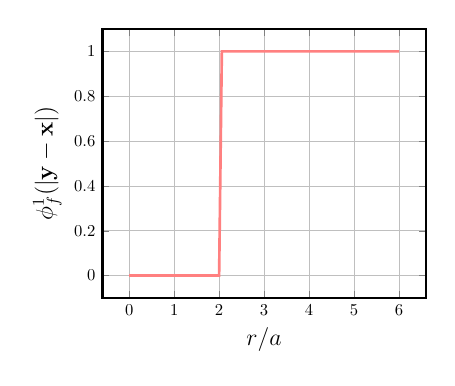
\begin{tikzpicture}[scale=0.6]
    \begin{axis}[
        xlabel={\Large$r/a$},
        ylabel={\Large$\phi_f^1(|\textbf{y}-\textbf{x}|)$},
        legend style={at={(0.05,0.05)}, anchor=south west},
        grid=major,
        domain=0:6,
        samples=100,
        ultra thick
    ]
    
    % Plot for phi = 0.05
    \addplot[color=red!50,ultra thick]
    { x < 2 ? 0 : 1};
    % \addlegendentry{$\phi = 0.05$}
    
    % % Plot for phi = 0.01
    % \addplot[color=blue!50,ultra thick]
    % { exp(-0.01 * (x^3 - 1))};
    % \addlegendentry{$\phi = 0.01$}
    
    % % Plot for phi = 0.001
    % \addplot[color=green!50,ultra thick]
    % { exp(-0.0001 * (x^3 - 1))};
    % \addlegendentry{$\phi = 10^{-4}$}
    
    \end{axis}
\end{tikzpicture}


In that case we must treat the problem into three region 
\paragraph*{First : $|\textbf{y} - \textbf{x}| > 2a$ :} we have $\phi_f^1 = \phi_f$, thus, $\phi_f^{1d} = 0$. same for $\phi_d$
\begin{align*}
    \avg{(\delta_1 - P_1)\rho^0\textbf{w}}
    &=0\\
    \avg{(\delta_1 - P_1)\rho^0\textbf{u}^0} / P_1
    &= 
    % \avg{(\delta_1 - P_1)\rho_f\chi_f\textbf{u}^0_f}
    % \avg{(\delta_1 - P_1)\rho_d\chi_d\textbf{u}^0_d}
    % = 
    \rho_f\phi_f\textbf{u}^{1d}_f
    + 
    \rho_d\phi_d\textbf{u}^{1d}_d
    \\
    \avg{(\delta_1 - P_1)\bm\sigma^0} 
    &= 
    - \phi_f^1 p^{1d}_f\bm\delta P_1 
    +\mu_f P_1 (\grad \textbf{u}^{1d} + \grad \textbf{u}^{1d})
    + \avg{(\delta_1 - P_1) \chi_d\bm\sigma^0_d}
\end{align*}
My guess is $\rho_f\phi_f\textbf{u}^{1d}_f
+ 
\rho_d\phi_d\textbf{u}^{1d}_d = \textbf{u}^{1d}$ 

and indeed we have 
\begin{equation*}
    \avg{\delta_1\textbf{u}^0} - \textbf{u}P_1
    = \avg{\delta_1 \chi_f \textbf{u}_f^0 + \chi_d \textbf{u}_d^0\delta_1 }
    - \textbf{u}_f\phi_fP_1
    - \textbf{u}_d\phi_dP_1
    \approx
    \phi_f^1 \textbf{u}_f^{1d} 
    + \phi_d^1 \textbf{u}_d^{1d}
\end{equation*}

\subsubsection*{Computation of the fluid phase term}

For suspension of spherical particles in the dilute limit the fluid phase averaged fields may be simplyfied by noticing that $\phi_f^1[\textbf{x},t;\textbf{y},\textbf{c}] P_1[\textbf{y},\textbf{c},t] = P_1[\textbf{y},\textbf{c},t]$ when $|\textbf{x} - \textbf{y}| > a$. 
\begin{equation}
    \avg{\chi_f f_f^0}[\textbf{x},t]
    = 
    \int_{\mathbb{R}^3}
    \int_{\mathbb{R}^3}
    f_f^1 \phi_f^1[\textbf{x},t;\textbf{y},\textbf{c}] P_1[\textbf{y},\textbf{c},t]
    d\textbf{y} 
    d\textbf{c}
\end{equation}
where,
\begin{equation*}
    f_f^1 \phi_f^1[\textbf{x},t;\textbf{y},\textbf{c}] P_1[\textbf{y},\textbf{c},t]
    =     
    \int
    \frac{1}{N}
    \sum_\alpha \delta(\textbf{y}-\textbf{x}_\alpha)
     \delta(\textbf{c}-\textbf{u}_\alpha)
    \chi_f
    f^0_f[\textbf{x},t;\FF]
    d\PP.
\end{equation*}

% \section{Introduction}
\label{ap:Closure_problem}

The equations governing the closure problem are often derived based on physical principles or intuitive reasoning.
For example, to determine the drag force term in the averaged momentum equation, in the dilute limit, the problem of a translating sphere in an unbounded flow with background velocity $\textbf{u}^\infty$ is commonly considered \citep{stone2001inertial,raja2010inertial,guazzelli2011}.
"background velocity" refers to the undisturbed flow at the particle location as if the particle were not present.


However, in the context of averaged equations, one might wonder: does $\textbf{u}^\infty$ correspond to the averaged fluid velocity $\textbf{u}_f$ (as used in \citet{jackson1997locally,zhang1997momentum}), the bulk velocity $\textbf{u}$ \citep{kim1985modelling}, or the Favre-averaged velocity $\textbf{u}_m$?
In other words, how can we relate the ensemble-averaged properties of the "hybrid" or "two-fluid" model to the closure terms?

As demonstrated, this question introduces the need for a rigorous statistical derivation of the closure problem.

The closure terms in the ``Hybrid'' model are the results of the ensemble average operator $\avg{\ldots}$. 
In all rigor, we cannot compute theoretically such an average since it necessitates knowing the distribution $P(\FF)$ and the exact expression of the local terms indicated by the notation $(\ldots)^0$. 
In the same spirit as in \citet{buyevich1979flow,lhuillier1992ensemble,batchelor1972sedimentation,hinch1977averaged} and \citet{zhang1994averaged} we demonstrate here that it is therefore necessary to reformulate the closure term to remove the ensemble average procedure. 
We demonstrated in \ref{ap:Closure_problem} that any ensemble-averaged quantities can be reformulated as an integral of what we call \textit{conditionally-averaged quantities}. 
The expressions obtained are  consistent with \citet{batchelor1972sedimentation,hinch1977averaged} and \citet[Appendix A]{zhang1994averaged} which also proposed conditional averages, but somewhat more general because our methodology applies to any closure term of the ``Hybrid model''. 
In a second step, we demonstrate how to derive what we call the \textit{conditionally-averaged equations} that are needed to obtain the \textit{conditionally-averaged quantities}. 

In the limit of Stokes flows \citet{hinch1977averaged} were the first authors to introduce this methodology.
He used the \textit{conditionally-averaged equations} to re-demonstrate, as a proof of concept, the bulk stress of a suspension of solid spheres at $\mathcal{O}(\phi^2)$ and the sedimentation velocity of the dispersed phase at $\mathcal{O}(\phi^2)$. 
In \citet{kim1985modelling} they use the \textit{conditionally-averaged equations} to consider the effect of finite volume fraction on the drag force closure term, in fixed beds of spherical solid spheres, their analysis holds for arbitrary volume fraction $\phi$. 

Again our derivation is directly inspired by the cited author, but the approach is generalized by considering fluid inclusion and an inertial regime. 
For instance, in the dilute regime, the \textit{conditionally-averaged equations} correspond to the problem of the disturbance field generated by an isolated translating droplet. 
The real interest behind this demonstration is that it is kept general and offers many possibilities for model extension.
 




% In \ref{sec:reformulation} and \ref{sec:the_disturbance_eq} we discuss the general approach to derive the closure problem
%%%%%%%%%%%%%%%%%%% A mettre dans lautre chap
% , while in \ref{sec:application} we derive the closures terms of the momentum and energy equations. 
% Since the derivation of the closure terms can be understood through physical arguments, readers who are less interested in the rigorous mathematical formulation of the closure problem, which can be quite involved, may skip directly to \ref{sec:application}.


\section{Reformulation of the closure terms}
\label{sec:reformulation}

% We aim to compute our closures within the dilute Stokes flow regime for spherical particles of radius $a$. 
% In this regime we expect that the closure terms will only be determined by the center of mass velocity of the droplets ($\textbf{u}_p$), their position in space, and the macroscopic properties of the continuous phase ($\textbf{u}_f, \grad \textbf{u}_f \ldots$). 
% Indeed, as we will demonstrate in the following section, only these properties define the boundaries of the \textit{single-particle} conditionally-averaged equations, and are therefore sufficient to achieve closure of the problem  in the Stokes flow regime. 

In the following, we express our closures in terms of averaged quantities, conditioned on the position of the center of mass of a \textit{test-particle} and its center of mass velocity. 
Note that for shape-dependent closure terms it would also be necessary to obtain the \textit{shape-conditioned} averaged fields, but this is out of the scope of this work.
Similarly, to account for the contribution of droplet acceleration to the closure terms (such as the added mass effect), it would be necessary to consider the \textit{center-of-mass-acceleration-conditioned} averaged fields.
However, this lies beyond the scope of the present work.
  
\subsection{Interfacial terms}

In the equations presented in \ref{sec:application} certain closures, such as surface stresses and surface heat fluxes, are expressed in the form of particle-averaged surface integrals. 
Here, we focus on reformulating these terms in terms of \textit{single-particle} conditionally-averaged quantities, which will be defined in the subsequent sections.

As the procedure is similar for all surface particle-averaged terms, let us take the example of the exchange of momentum term appearing in the continuous and dispersed phase averaged momentum equations (\ref{eq:dt_hybrid_rhou_f} and \ref{eq:dt_hybrid_up}). 
From the definition of the particle average we write,
\begin{align}
    \pSavg{\bm\sigma_f^0\cdot\textbf{n}}[\textbf{x},t]
    &= \avg{ \sum_{\alpha=1}^N \delta(\textbf{x}-\textbf{x}_\alpha[t; \FF])
    \int_{\Gamma_\alpha(t,\FF)}
    (\bm\sigma_f^0\cdot\textbf{n})[\textbf{y},t;\FF]
    d\Gamma[\textbf{y}] }
    \label{eq:first_step_reallay}
\end{align}
By writing this integral explicitly, we emphasize that the particle-averaged quantity (left-hand side of \ref{eq:first_step_reallay}) is evaluated at the point \textbf{x}, while the parameter $\textbf{y}$ is used for the integration over the particle's surface.
Recall that $\Gamma_\alpha$ refers to the surface of the droplet $\alpha$ and $\textbf{x}_\alpha$ to the position of the center of mass of that same droplet $\alpha$. 
Thus, the notation $(\bm\sigma_f^0\cdot\textbf{n})[\textbf{y},t;\FF]$ means that we evaluate the local stress as well as the local normal $\textbf{n}$ to the particle surface, at \textbf{y}. 
We now enlarge the domain of integration from $\Gamma_\alpha$ (the surface of the particle $\alpha$) to $\mathbb{R}^3$ with the introduction of the interface indicator function of the particle $\alpha$, namely $\delta(|\textbf{y} - \textbf{x}_\alpha[t,\FF]| - a)$\footnote{Indeed, for spherical particles, we can define the interface indicator function of a single particle using the definition $\delta_\Gamma = \delta(|\textbf{y} - \textbf{x}_\alpha[t,\FF]| - a)$.}. 
It reads,
\begin{multline}
    \pSavg{\bm\sigma_f^0\cdot\textbf{n}}[\textbf{x},t]
    = \\
    \int_{\mathbb{R}^3}
    \avg{
     \sum_{\alpha=1}^N 
     \delta(\textbf{x}-\textbf{x}_\alpha[t \FF])
    \delta(|\textbf{y} - \textbf{x}_{\alpha}[t;\FF]|-a)
    (\bm\sigma_f^0\cdot\textbf{n})[\textbf{y},t;\FF]
    }
    d\textbf{y}. 
    \label{eq:first_step_drag}
\end{multline} 
Since the domain of integration $\mathbb{R}^3$ is now independent of $\FF$, we may substitute the integral and ensemble average operator. 

As mentioned above, we assume that the closure terms are entirely determined by the center of mass velocity of the particles and their position in space. 
Therefore, to include the condition on the particle velocity we introduce the relation 
\begin{equation}
    \int_{\mathbb{R}^3} \delta(\textbf{w} - \textbf{u}_\alpha[\FF,t]) d\textbf{w} = 1,
    \label{eq:Pw_normed}
\end{equation}
where $\textbf{w}$ is the test-particle center of mass velocity in the Eulerian space and $\textbf{u}_\alpha$ is the center of mass velocity within the Lagrangian framework. 
Injecting \ref{eq:Pw_normed} into \ref{eq:first_step_drag} one obtains, 
\begin{multline}
    \pSavg{\bm\sigma_f^0\cdot\textbf{n}}[\textbf{x},t]
    = \\
    \int_{\mathbb{R}^3}
    \int_{\mathbb{R}^3}
    \avg{
     \sum_{\alpha=1}^N 
     \delta(\textbf{x}-\textbf{x}_\alpha[t \FF])
     \delta(\textbf{w} - \textbf{u}_\alpha[\FF,t])
    \delta(|\textbf{y} - \textbf{x}_{\alpha}[t;\FF]|-a)
    (\bm\sigma_f^0\cdot\textbf{n})[\textbf{y},t;\FF]
    }
    d\textbf{y}
    d\textbf{w}. 
    \label{eq:second_step_drag}
\end{multline}
The quantity with the ensemble average operator now represents the average of the local stress $(\bm\sigma_f^0\cdot\textbf{n})[\textbf{y},t;\FF]$ on every configuration where the interface of a droplet is present at \textbf{y} with its center of mass at \textbf{x} and with a center of mass velocity \textbf{w}.


Moreover, since the expression within the ensemble average in \ref{eq:first_step_drag} is identically zero when, $\textbf{x}_\alpha \neq \textbf{x}$, we may replace the interface indicator function such that 
\begin{equation}
    \delta(\textbf{x}-\textbf{x}_\alpha[t,\FF])\delta(|\textbf{y} - \textbf{x}_{\alpha}[t,\FF]|-a) = \delta(\textbf{x}-\textbf{x}_\alpha[t,\FF])\delta(|\textbf{y} - \textbf{x}|-a). 
    \label{eq:from_R3_to_S}
\end{equation}
Since the function $\delta(|\textbf{y} - \textbf{x}|-a)$ is not dependent on $\FF$ it can be taken out of the ensemble average operator, hence reducing the domain of integration from $\mathbb{R}^3$ to $|\textbf{y}-\textbf{x}| = a$ in \ref{eq:first_step_drag}. 
\footnote{For deformable or non-spherical particles, this function may take a more complicated form, since the interface of a deformable or anisotropic particle is not entirely determinate by its center of mass position. 
It is clear that if the position of the interface is conditioned by the exact shape of the interface, then we can always express the interface indicator function as $\delta(f(\textbf{x}))$ where $f$ is a distance function of the shape that may depend on the particle's orientation (for anisotropic particles) or aspect ratio (for slightly deformable ones). 
Anyhow, this approach is generalizable to other kinds of particles, but in this work, we consider only spherical droplets. 
Note that for spheroidal particles as in \ref{chap:deformable} we may write $\delta_{\alpha\Gamma} = \delta((\textbf{y} - \textbf{x}_\alpha[t,\FF])\cdot (\bm\chi_\alpha+\bm\delta)\cdot(\textbf{y} - \textbf{x}_\alpha[t,\FF]) - a^2)$ where we have used the notation of \ref{chap:deformable}
}

Injecting \ref{eq:from_R3_to_S} into \ref{eq:second_step_drag} and using the last remark leads us to the relation 
\begin{equation}
    \pSavg{\bm\sigma_f^0\cdot\textbf{n}}[\textbf{x},t]
    =
    \int_{\mathbb{R}^3}
    P_1[\textbf{x},\textbf{w},t]
    \int_{|\textbf{x}-\textbf{y}|=a}
    (\bm\sigma_f^1 \cdot \textbf{n})[\textbf{y},\textbf{x},\textbf{w},t]
    d\textbf{y}
    d\textbf{w}
    \label{eq:conditionally_averaged}
\end{equation}
where we introduced the definitions, 
\begin{align}
    \bm\sigma^1_f[\textbf{y},\textbf{x},\textbf{w},t]
    % \phi_I^1[\textbf{y}|\textbf{x},\textbf{w},t] 
    % P_1[\textbf{x},\textbf{w},t]
    &= 
    \frac{1}{P_1}
    \avg{
    \sum_\alpha^N 
    \delta(\textbf{x} - \textbf{x}_\alpha[t,\FF])
    \delta(\textbf{w} - \textbf{u}_\alpha[t,\FF])
    % \delta(|\textbf{y} - \textbf{x}_{\alpha}[t,\FF]|-a)
    \bm\sigma_f^0[\textbf{y},t,\FF]
    },
    \label{eq:sigma_f_1}
    \\
    % \phi_I^1[\textbf{y}|\textbf{x},\textbf{w},t] 
    % P_1[\textbf{x},\textbf{w},t]\nonumber\\
    % = 
    % \avg{
    % \sum_\alpha^N 
    % \delta(\textbf{x} - \textbf{x}_\alpha[t,\FF])
    % \delta(\textbf{w} - \textbf{u}_\alpha[t,\FF])
    % \delta(|\textbf{y} - \textbf{x}_{\alpha}[t,\FF]|-a)
    % }\\
    P_1[\textbf{x},\textbf{w},t]
    &= 
    \avg{
    \sum_\alpha^N 
    \delta(\textbf{x} - \textbf{x}_\alpha[t,\FF])
    \delta(\textbf{w} - \textbf{u}_\alpha[t,\FF])
    }. 
\end{align}
% \tb{Since we reduced the surface int the stress isn't any more conditioned by the surface }
% Here $\bm\sigmais the \textit{single-particle} conditionally-averaged local stress of the continuous phase knowing that interface of the particle at $\textbf{x}$ is  present in \textbf{y} and that there is a particle at \textbf{x} with velocity \textbf{w}. 
With this definition, $\bm\sigma^1_f$ is the continuous phase stress, evaluated at $\textbf{y}$ and time $t$, knowing that there is a particle at position $\textbf{x}$ with velocity \textbf{w}, and that the point \textbf{y} is occupied by the surface of the test-particle 
\footnote{
    As $\bm\sigma^1_f$ is conditioned on the variables: $\textbf{y}$, $\textbf{x}$, $\textbf{w}$, $t$, and evaluated at the position $\textbf{y}$ and time $t$, we should write: $\bm\sigma^1_f[\textbf{y},t|\textbf{x},\textbf{y},\textbf{w},t]$ instead of $\bm\sigma^1_f[\textbf{x},\textbf{y},\textbf{w},t]$.
    However the second notation will be used as a short hand. 
}.
% $\phi_I^1[\textbf{y}|\textbf{x},\textbf{w},t] $ is the probability of finding the interface of the particle at the location \textbf{y} knowing its center of mass is located at \textbf{x}. 
% For identical spherical particles we can write $\phi_I^1[\textbf{y}|\textbf{x},\textbf{w},t] = \delta(|\textbf{x} - \textbf{y}| -a)$.
% That is why the domain of integration over \textbf{y} in \ref{eq:conditionally_averaged} is reduced to $|\textbf{x} - \textbf{y}| < a$. 
$P_1[\textbf{x},\textbf{w},t]$ is the probability of finding a particle center of mass at \textbf{x} with velocity \textbf{w} at time $t$.
This distribution can be decomposed such that $P_1[\textbf{x},\textbf{w},t] = n_p[\textbf{x},t] P_1[\textbf{w}|\textbf{x},t]$ where $n_p$ is the number density evaluated at \textbf{x}, and $P_1$ the probability density of having a particle with velocity \textbf{w} knowing its center of mass location is \textbf{x}. 
Note that this distribution is normed 
\begin{equation*}
    \int_{\mathbb{R}^3} P_1[\textbf{w}|\textbf{x},t] d \textbf{w} = 1. 
\end{equation*}
Finally, note that in \ref{eq:conditionally_averaged} the droplet shape and the position of its center of mass fully determine the normal vector $\textbf{n}$, allowing it to be taken outside the ensemble average. 


\subsubsection{Single-particle conditionally averaged quantities}

All quantities denoted with the superscript $^1$ refer to \textit{single-particle} conditionally-averaged quantities. 
These quantities are conditionally averaged based on the presence of a particle located at \textbf{x} with velocity \textbf{w}.
Additionally, in the following, we will use the shorthand,
\begin{equation}
    \delta_1[\textbf{x},\textbf{w},t,\FF]  \text{ for } \sum_\alpha \delta(\textbf{x} - \textbf{x}_\alpha[t,\FF]) \delta(\textbf{w} - \textbf{u}_\alpha[t,\FF]). 
    \label{eq:delta_1}
\end{equation}  
Thus, we can define the \textit{single-particle} conditional-average of a local quantity $f^0$, as 
\begin{equation}
    f^1[\textbf{y}|\textbf{x},\textbf{w},t] P_1[\textbf{x},\textbf{w},t] = \avg{\delta_1 f^0[\textbf{y},\FF,t]}.
\end{equation}
Such that $f^1$ is the averaged value of $f^0$ at \textbf{y} knowing that there is a particle at \textbf{x} with velocity \textbf{w}. 
If $f_k$ is a quantity defined in the phase $k$ we may write 
\begin{equation*}
    f^1_k[\textbf{y}|\textbf{x},\textbf{w},t] \phi_k^1[\textbf{y}|\textbf{x},\textbf{w},t]  P_1 = \avg{\delta_1 (\chi_k f^0_k) [\textbf{y},\FF,t]}.
\end{equation*}
Such that $\phi_k^1$ is the probability of finding the phase $k$ at \textbf{y} knowing a particle is located at \textbf{w} with velocity \textbf{w}, and $f_k^1$ the conditional average of $f_k^0$. 
For example, we define the \textit{single-particle conditioned average} of the continuous phase velocity fields by, 
\begin{equation*}
    \textbf{u}_f^1 \phi_f^1 P_1
    = \avg{\delta_1 \chi_f \textbf{u}_f^0}
\end{equation*} 
where $\phi_f^1$ is the probability of finding the continuous phase at \textbf{y} knowing a particle is present at \textbf{x} with velocity \textbf{w}. 
$\textbf{u}_f^1$ is the averaged local velocity evaluated at \textbf{y} knowing the continuous phase is present at \textbf{y} with a particle at \textbf{x} having velocity \textbf{w}. 

The stress present in \ref{eq:conditionally_averaged} can now be expressed in terms of conditionally-averaged velocity and pressure fields. 
We use the constitutive law of Newtonian fluids, $\bm\sigma_f^0 = -p_f^0 \bm\delta + \mu_f [\pddy \textbf{u}_f^0+ (\pddy \textbf{u}_f^0)^\dagger]$, with $\pddy$ the gradient over the \textbf{y} coordinate.
Injecting this law into \ref{eq:sigma_f_1} we obtain directly 
\begin{equation}
    \bm\sigma_f^1
    = - p_f^1 \bm\delta
    +\mu_f [\pddy \textbf{u}_f^1+(\pddy \textbf{u}_f^1)^\dagger], 
    \label{eq:sigma_f_surf}
\end{equation}
since $\delta_1$ is independent of \textbf{y}, meaning that it could be permuted with the gradient operator in \ref{eq:sigma_f_surf}. 
Note that this relation is valid only because $\bm\sigma_f^1$ is conditioned on the presence of an interface at \textbf{y} in \ref{eq:sigma_f_1}. 
In conclusion, the ensemble averaged exchange of momentum term can be expressed as the surface integral of the Newtonian stress defined based on the \textit{single-particle} conditional-averaged fields: $\textbf{u}_f^1$, and $p_f^1$. 

It must be understood that this definition \eqref{eq:sigma_f_surf} is only true because the stress is evaluated at the surface of the droplet, in the general case we have, 
\begin{equation}
    P_1 \phi_f^1 \bm\sigma_f^1
    =
    \avg{\delta_1 \chi_f \bm\sigma_f^0}
    =
    P_1 \phi_f^1 p_f^1
    +  \avg{\delta_1\chi_f \{ - p_f^0 \bm\delta + \mu_f [\pddy \textbf{u}_f^0+  (\pddy \textbf{u}_f^0)^\dagger]\}}. 
    \label{eq:sigme_f_1_all_space}
\end{equation}
Note the presence of $\chi_f$ in this expression, in opposition to \ref{eq:sigma_f_surf} where only $\delta_1$ where present.
This is because \ref{eq:sigme_f_1_all_space} is evaluated at an arbitrary point \textbf{y}, while in \ref{eq:sigma_f_surf} we consider only the points lying on the droplet interface.  
From this expression, we can propose two formulations for the continuous phase stress,   
\begin{align}    
    \bm\sigma_f^1
    &= 
    - p_f^1 \bm\delta 
    + \mu_f [\pddy \textbf{u}_f^1+ (\pddy \textbf{u}_f^1)^\dagger ]
    - \frac{\mu_f }{P_1 \phi_f^1}\avg{\delta_1 \delta_\Gamma (\textbf{n}_d \textbf{u}_f''+  \textbf{u}_f'' \textbf{n}_d)},
    \label{eq:sigma_f_surf15}
    \\
    \bm\sigma_f^1
    &= 
    - p_f^1 \bm\delta 
    + \frac{\mu_f }{\phi_f^1} [\pddy \textbf{u}^1+ (\pddy \textbf{u}^1)^\dagger ]
    - \frac{\mu_f }{\phi_f^1} \phi_d^1 \textbf{e}_d^1. 
    \label{eq:sigma_f_surf2}
\end{align}
Where we have defined $\textbf{u}_f'' = \textbf{u}_f^0 - \textbf{u}_f^1$. 
These two expressions can be derived using a similar methodology than for the derivation of \ref{eq:second_form,eq:first_form}. 
Note that the second term on the right-hand side of \ref{eq:sigma_f_surf2} vanishes for solid particles, the rate of strain within solid particle is null.
While the second term of \ref{eq:sigma_f_surf15} does not necessarily vanish. 
That is why the second expression is preferred for solid particles. 

% Additionally, multiplying \ref{eq:sigma_f_surf15} and \ref{eq:sigma_f_surf2} by $\phi_f^1$ and subtracting both expressions gives, 
% \begin{equation} 
%     \frac{1}{P_1}\avg{\delta_1 \delta_\Gamma (\textbf{n}_d \textbf{u}_f''+  \textbf{u}_f'' \textbf{n}_d)}
%     -  \phi_d^1 \textbf{e}_d^1
%     = 
%     [(\textbf{u}_f^1 - \textbf{u}_d^1)\pddy\phi_d^1+ \pddy \phi_d^1(\textbf{u}_f^1 - \textbf{u}_d^1) ]
%     - \phi_d^1 [\pddy\textbf{u}_d^1+  (\pddy \textbf{u}_d^1)^\dagger ]. 
% \end{equation}
% For ensemble averaged (not conditionally-averaged) quantities we can equally show that
% \begin{multline} 
%     \avg{\delta_\Gamma (\textbf{n}_d \textbf{u}_f'+  \textbf{u}_f' \textbf{n}_d)}
%     - \phi_d \textbf{e}_d
%     = 
%     +  [(\textbf{u}_f - \textbf{u}_d)\pddy\phi_d+ \pddy \phi_d(\textbf{u}_f - \textbf{u}_d) ]
%     - \phi_d [\pddy\textbf{u}_d+  (\pddy \textbf{u}_d)^\dagger ]
% \end{multline}
% Note that for solid particles this relation can directly lead us to a closure for the surface term on the left-hand side, namely
% \begin{multline} 
%     \avg{\delta_\Gamma (\textbf{n}_d \textbf{u}_f'+  \textbf{u}_f' \textbf{n}_d)}
%     = 
%     [(\textbf{u}_f - \textbf{u}_d)\pddy\phi_d+ \pddy \phi_d(\textbf{u}_f - \textbf{u}_d) ]
%     - \phi_d [\pddy\textbf{u}_d+  (\pddy \textbf{u}_d)^\dagger ]. 
%     \label{eq:closure_un_nu}
% \end{multline}

\begin{figure}[h!]
    \centering
    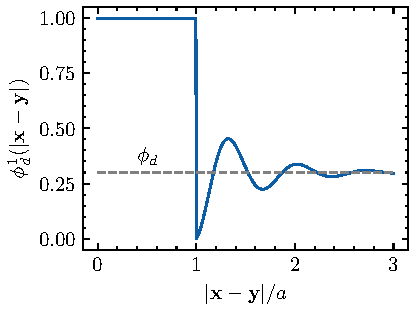
\includegraphics[width=0.2\textheight]{image/dist_phi.pdf}
    \caption{Representation of a possible form for the probability of finding the dispersed phase at \textbf{x} knowing a spherical particle of radius $a$ is present at $\textbf{y}$.
    Note the zone empty of particle concentration near the points $|\textbf{x}- \textbf{y}|=a$, this due to the impenetrability of particles. 
    }
    \label{fig:distrib}
\end{figure}
At the surface of the test-particle, the probability of finding the dispersed phase, i.e. finding the dispersed phase in contact with the surface of the reference particle, is identically null (not to be confused with the probability of finding another droplet center of mass). 
Indeed, a thin film of continuous phase always separates the droplet surface from its neighbors (see \ref{fig:distrib}).
Therefore, we may write $\phi_d^1 = 0$ at $|\textbf{x}- \textbf{y}| =a$. 
Thus, when evaluated at the subsurface of the particle, we can use the relation $\textbf{u}_f^1 = \textbf{u}^1$ and $p_f^1 = p^1$. 
Consequently, to compute the surface stress of a particle, either the conditionally-averaged quantities of the continuous phase ($\textbf{u}_f^1, p_f^1$) or the bulk quantities ($\textbf{u}^1$, $p^1$) are required. 
Another consequence of this is that, the definitions given by, \ref{eq:sigma_f_surf15}, \ref{eq:sigma_f_surf2}, or \ref{eq:sigma_f_surf} are all consistent when evaluated at the points located on the surface of the droplet at \textbf{x}. 

\subsection{Mean fields and disturbance fields contribution}

As it is often done in the literature \citep{zhang1994ensemble,jackson2000,wang2021numerical,wang2024effect}, we would like to separate the averaged momentum exchange into a contribution from the mean flow and pressure fields, and the contribution arising due to the disturbance velocity and pressure fields.  

\subsubsection{Definitions}

In the first place, we need to define what is a disturbance field.
Let us take the example of the conditioned velocity field, $\textbf{u}_f^1$, and its corresponding disturbance velocity field.
We state that the conditioned field, $\textbf{u}_f^1$, is equivalent to the ensemble-averaged velocity field $\textbf{u}_f$ when the particle at \textbf{x} is sufficiently far from the point where the velocity $\textbf{u}_f^1$ is evaluated (the point \textbf{y}).
Thus, we write,  
\begin{equation}
    \lim_{|\textbf{y}-\textbf{x}|\to\infty} 
    \textbf{u}_f^1[\textbf{y},\textbf{x},\textbf{w},t]
    =
    \textbf{u}_f[\textbf{y},t]. 
    \label{eq:lim_u_1}
\end{equation} 
Note that this definition requires an infinitely large domain. 
This implies that the solutions obtained in the subsequent sections are restricted to infinitely large domains, devoid of boundary conditions.

Let us assume that $L$ is the macroscopic length scale of our process and that $a$  is the typical size of the particles.
Since the particle-size scale $a$ is much smaller than the boundary length scale $L$ we assume that $\textsc{O}(a/L)$ is negligible. 
In the worth case scenario, the disturbance field of a droplet is $(\textbf{u}_f^1- \textbf{u}_f)\sim a/|\textbf{y}-\textbf{x}|$ \citet{kim2013microhydrodynamics}.
Hence, in a physical situation where $|\textbf{y}-\textbf{x}|\to L$ instead of $|\textbf{y}-\textbf{x}|\to\infty$ in \ref{eq:lim_u_1} we may estimate that the error is of $\mathcal{O}(a/L)$, hence negligible upon a reasonable separation of scale.
However, it is interesting to note that this will no longer be the case for other problems such as sediment transport for examples.
In this case, the boundary condition, i.e. the top of the particle bed and the ground, are at a distance of the same length scale as the particle-size. 

In light of \ref{eq:lim_u_1}, we define the disturbance velocity field as 
\begin{equation}
    \textbf{u}_f^{1d}
    =
    \textbf{u}_f^1 
    - 
    \textbf{u}_f. 
    \label{eq:def_u_1d}
\end{equation}
because it satisfies the definition, 
\begin{equation}
    \lim_{|\textbf{y}-\textbf{x}|\to\infty} 
    \textbf{u}_f^{1d}[\textbf{y},\textbf{x},\textbf{w},t]
    =
    \lim_{|\textbf{y}-\textbf{x}|\to\infty} 
    \{\textbf{u}_f^1[\textbf{y},\textbf{x},\textbf{w},t]
    - \textbf{u}_f[\textbf{y},t]\}
    = 0.
    \label{eq:lim_u_1d}
\end{equation} 
Thus, $\textbf{u}_f^{1d}$ tends to zero at large distances from the particle, which is consistent with the terminology ``disturbance''.
The definition \ref{eq:def_u_1d} can apply to any \textit{conditional-averaged} quantities $f^1$, we define
\begin{equation}
    \lim_{|\textbf{y}-\textbf{x}|\to\infty} 
    \{f_f^1[\textbf{y},\textbf{x},\textbf{w},t]
    - f_f[\textbf{y},t]\}
    =
    f_f^{1d}[\textbf{y},\textbf{x},\textbf{w},t]
    = 0.
\end{equation} 

\subsubsection{Momentum exchange decomposition}

Using the decomposition $\bm\sigma_f^1 = \bm\sigma_f^{1d} + \bm\sigma_f$ in \ref{eq:conditionally_averaged} we finally introduce the decomposition of the averaged momentum exchange term as:  
\begin{align}
    \pSavg{\bm\sigma_f^0\cdot\textbf{n}}[\textbf{x},t]
    =
    n_p[\textbf{x},t]
    \int_{|\textbf{x}-\textbf{y}|=a}
    \bm\sigma_f[\textbf{y},t]
    \cdot \textbf{n}
    d\textbf{y}
    \nonumber
    \\
    + 
    \int_{\mathbb{R}^3}
    P_1[\textbf{x},\textbf{w},t]
    \int_{|\textbf{x}-\textbf{y}|=a}
    \bm\sigma_f^{1d}[\textbf{y},\textbf{x},\textbf{w},t]
    \cdot \textbf{n}
    d\textbf{y}
    d\textbf{w}
    \label{eq:general_partition}
\end{align}
where the first term represents the contribution from the mean continuous phase stress, $\bm\sigma_f$, and the second term is the contribution from the disturbance fields stress $\bm\sigma_f^{1d}$. 
While this decomposition is arbitrary since $\bm\sigma_f^1$ could be partitioned into other arbitrary tensors, it enables by definition, the separation of the mean flow contribution, $\bm\sigma_f$, from the stress induced by the local-scale disturbance fields, $\bm\sigma_f^{1d}$.
This decomposition is used by \citet[Chapter 2]{jackson2000} and \citet{zhang1997momentum,wang2021numerical,wang2024effect} for suspensions of solid spheres, although these authors do not explicitly provide the expression for the tensor $\bm\sigma_f^{1d}$, which we aim to derive in the following sections. 

Note that $\bm\sigma_f$ is evaluated at $\textbf{y}$ in \ref{eq:general_partition}. 
Although $\bm\sigma_f$ is ensemble-averaged, we emphasize that it may still depend on the position in inhomogeneous flows. 
Assuming the suspension is slightly non-homogeneous \citep{lhuillier1992ensemble}, we have $\bm\sigma_f[\textbf{y},t] = \bm\sigma_f[\textbf{x},t] + \textbf{r}\cdot \nabla\bm\sigma_f[\textbf{x},t] + \ldots$, where $\textbf{r} = \textbf{y} - \textbf{x}$. 
By retaining only the first three terms in the expansion, we can demonstrate that
\begin{equation}
    \pSavg{\bm\sigma_f^0\cdot\textbf{n}}
    =
    n_p v_p 
    \div\bm\sigma_f
    +
    \int_{\mathbb{R}^3}
    P_1
    \int_{|\textbf{x}-\textbf{y}|=a}
    \bm\sigma_f^{1d} \cdot \textbf{n}
    d\textbf{y}d\textbf{w}.
    \label{eq:drag_final}
\end{equation}
Therefore, the total momentum exchange term contains a component related to the divergence of the mean fluid-phase stress, in addition to the contribution from the disturbance fields. 
Similar arguments can be extended to the first two moments of the hydrodynamic force. 
These expressions can be written as:
\begin{align}
    \pSavg{\textbf{r}\bm\sigma_f^0\cdot\textbf{n}}
    &=
    n_p v_p \bm\sigma_f
    +
    \int_{\mathbb{R}^3}
    P_1
    \int_{|\textbf{x}-\textbf{y}|=a}
    \textbf{r}\bm\sigma_f^{1d} \cdot \textbf{n}
    d\textbf{y}
    d\textbf{w},
    \label{eq:first_mom_general}
    \\
    \pSavg{\textbf{rr}\bm\sigma_f^0\cdot\textbf{n}}
    &=
    n_pv_p  \frac{a^2}{5} 3 [(\div \bm\sigma_f)\bm\delta]^\text{sym}
    +
    \int_{\mathbb{R}^3}
    P_1
    \int_{|\textbf{x}-\textbf{y}|=a}
    \textbf{rr}\bm\sigma_f^{1d} \cdot \textbf{n}
    d\textbf{y}
    d\textbf{w},
    \label{eq:second_mom_general}
\end{align}
where the operator $[\ldots]^\text{sym}$ returns the symmetric part of the arguments. 
It is important to note that the contribution from the mean stress in the second moment of the hydrodynamic force may become negligible when a proper separation of scale is considered. 
Indeed, this term is proportional to $a^2$ \eqref{eq:second_mom_general}, and it appears under the operator $\grad\grad\sim L^{-2}$ in the averaged momentum equation \ref{eq:dt_hybrid_rhou_f}, hence contributing to $\mathcal{O}(a^2/L^2)$, which may be considered as negligible. 

According to the expressions \ref{eq:drag_final}, \ref{eq:first_mom_general}, and \ref{eq:second_mom_general}, we will need to compute the term $\bm\sigma^{1d}_f = \bm\sigma_f^1 - \bm\sigma_f$ where $\bm\sigma_f^1$ is given by \ref{eq:sigma_f_surf}. 
Regarding the mean continuous phase stress we recall that it can be written in two ways (see \ref{chap:daniel15}), namely 
\begin{align}
    \label{eq:mean_continuous_phase_stress}
    \bm\sigma_f
    &= - p_f \bm\delta 
    + \mu_f [\pddy \textbf{u}_f+ (\pddy \textbf{u}_f)^\dagger ]
    - \frac{\mu_f}{\phi_f}\avg{\delta_\Gamma (\textbf{n}_d \textbf{u}_f'+  \textbf{u}_f' \textbf{n}_d)}, \\
    \bm\sigma_f
    &= - p_f \bm\delta 
    + \frac{\mu_f}{\phi_f} [\pddy \textbf{u}+ (\pddy \textbf{u})^\dagger ]
    - \frac{\mu_f \phi_d}{\phi_f} \textbf{e}_d
    \label{eq:mean_continuous_phase_stress2}
\end{align}
Thus using \ref{eq:sigma_f_surf} and \ref{eq:mean_continuous_phase_stress} we find for the points on the particle's surface ($|\textbf{y}-\textbf{x}| = a$) that,
\begin{align}
    \bm\sigma_f^{1d}
    =
    - p_f^{1d} \bm\delta 
    + \mu_f [\pddy \textbf{u}_f^{1d}+ (\pddy \textbf{u}_f^{1d})^\dagger ]
    + \frac{\mu_f }{\phi_f}\avg{\delta_\Gamma (\textbf{n}_d \textbf{u}_f'+  \textbf{u}_f' \textbf{n}_d)}. 
    \label{eq:sigma_explict}
\end{align}
Thus, according to \ref{eq:sigma_explict}, the disturbance stress that is integrated over the particle surface in \ref{eq:drag_final} to \ref{eq:second_mom_general}, is not only the Newtonian stress-like contribution of the disturbance fields ($\textbf{u}_f^1$ and $p_f^1$), but also includes the contribution of the term $\avg{\delta_\Gamma (\textbf{n}_d \textbf{u}_f'+  \textbf{u}_f' \textbf{n}_d)}$. 
Thus, in the force closures: \ref{eq:drag_final} and \ref{eq:first_mom_general}, we will observe the appearance of the terms involving the divergence of $\avg{\delta_\Gamma (\textbf{n}_d \textbf{u}_f'+  \textbf{u}_f' \textbf{n}_d)}$ times $n_pv_p$, and  $n_pv_p \avg{\delta_\Gamma (\textbf{n}_d \textbf{u}_f'+  \textbf{u}_f' \textbf{n}_d)}$, respectively. 
These terms will ultimately cancel out their corresponding contributions in $\bm\sigma_f$ that appear on the left-hand side of \ref{eq:drag_final} and \ref{eq:first_mom_general}. 

To provide a better understanding for the following discussion we remark that for solid particles $\textbf{e}_d = 0$. 
Therefore, subtracting \ref{eq:mean_continuous_phase_stress} from \ref{eq:mean_continuous_phase_stress2}, gives directly, 
\begin{equation}
    \avg{\delta_\Gamma (\textbf{n}_d \textbf{u}_f'+  \textbf{u}_f' \textbf{n}_d)}
    = 
    (\textbf{u}_f - \textbf{u}_d)\pddy \phi_d + \pddy \phi_d (\textbf{u}_f - \textbf{u}_d)
    -  \phi_d [\pddy \textbf{u}_d+ (\pddy \textbf{u}_d)^\dagger ]. 
    \label{eq:closure_un_nu}
\end{equation} 
Therefore, at least for solid particles, this term is non-zero as soon as there are non-negligible gradients of volume fraction and mean gradients of particle velocities. 


We conclude that the commonly used decomposition of the drag force introduced by \citet{zhang1997momentum,jackson2000}, given by \ref{eq:general_partition}, requires adding the term  $\avg{\delta_\Gamma (\textbf{n}_d \textbf{u}_f'+  \textbf{u}_f' \textbf{n}_d)}$ to the classical Newtonian stresses in the second term of \ref{eq:general_partition} and subtracting it in the mean drag force term (first term of \ref{eq:general_partition}). 
This finding implies that, in the recent work of \citet{wang2021numerical, wang2024effect}, where this decomposition is employed for the drag force, we assert that they have actually computed the integral of the first two terms of \ref{eq:sigma_explict}, while neglecting the final term. 
Interestingly, \citet{wang2024effect} specifically investigates the effect of the volume fraction gradient ($\grad \phi_d$) on the drag force. 
In this context, it is clear from \eqref{eq:closure_un_nu} that the term $\avg{\delta_\Gamma (\textbf{n}_d \textbf{u}_f'+  \textbf{u}_f' \textbf{n}_d)}$ cannot be neglected. 
Only when the analysis is accurate to $\mathcal{O}(\phi_d)$ does this term vanish in \ref{eq:drag_final}, reducing \ref{eq:sigma_explict} to the Newtonian stress expression. 
% Thus, the drag force computed in the DNS of \citet{wang2024effect} may not be the one defined in their momentum equations. 

Note that using \ref{eq:mean_continuous_phase_stress2} instead of \ref{eq:mean_continuous_phase_stress} in \ref{eq:sigma_explict} and switching $\textbf{u}_f^1$ and $\textbf{u}^1$ in \ref{eq:sigma_f_surf}, does not solve this inconsistency. 

\subsubsection{An alternative stress decomposition}

As the previous decomposition requires adding and subtracting $\avg{\delta_\Gamma (\textbf{n}_d \textbf{u}_f'+  \textbf{u}_f' \textbf{n}_d)}$ in each term of \ref{eq:general_partition}, we decide to avoid this overcomplicated operation and introduce, the partitioning 
\begin{equation}
    \bm\sigma_f^1 =
    \bm\Sigma_f + 
    \bm\Sigma_f^{1d}. 
    \label{eq:mean_Newtonian}
\end{equation}
Where the mean stress and disturbance stresses are defined as, 
\begin{align}
    \bm\Sigma_f^{1d}
    &=-p_f^{1d}\bm\delta + \mu_f^1 [\grad \textbf{u}^{1d}_f + (\grad \textbf{u}^{1d}_f)^\dagger], \\
    \bm\Sigma_f
    &=-p_f\bm\delta + \mu_f^1 [\grad \textbf{u}_f + (\grad \textbf{u}_f)^\dagger], 
\end{align}
respectively. 
Note that the use of $\textbf{u}_f$ as the ensemble-averaged velocity of reference is arbitrary.
Indeed, recall that at the surface of the test particle we have $\phi_d^1=0$, hence $\textbf{u}_f^1 = \textbf{u}^1$. 
Thus, at the surface of the test-particle, one could use the decomposition,
\begin{equation}
    \bm\sigma_f^1 =
    \bm\Sigma + 
    \bm\Sigma^{1d}. 
    \label{eq:mean_Newtonian2}
\end{equation}
Where the mean stress and disturbance stresses are defined as, 
\begin{align}
    \bm\Sigma^{1d}
    &=-p_f^{1d}\bm\delta + \mu_f^1 [\grad \textbf{u}^{1d} + (\grad \textbf{u}^{1d})^\dagger], \\
    \bm\Sigma
    &=-p_f\bm\delta + \mu_f^1 [\grad \textbf{u} + (\grad \textbf{u})^\dagger]. 
\end{align}
One could wonder which of these stress decomposition (\ref{eq:mean_Newtonian2} or \ref{eq:mean_Newtonian}) is the more efficient? 
The answer is that it depends on the unknown of the problem at hand. 
If we consider an averaged system of equations for the mean continuous phase field $\textbf{u}_f$ then, \ref{eq:mean_Newtonian} seems more adapted, however, if the unknown is \textbf{u}, then \ref{eq:mean_Newtonian2} is more adapted. 
In all case since $\textbf{u} = \textbf{u}_f + \phi_d (\textbf{u}_d - \textbf{u}_f)$ one can always recover \ref{eq:mean_Newtonian2} from \ref{eq:mean_Newtonian} or inversely.




Using the same methodology as in the previous manipulations we re-write the force closures as, 
\begin{align}
    \pSavg{\bm\sigma_f^0\cdot\textbf{n}}
    &=
    n_p v_p 
    \div\bm\Sigma_f
    +
    \int_{\mathbb{R}^3}
    P_1
    \int_{|\textbf{x}-\textbf{y}|=a}
    \bm\Sigma_f^{1d} \cdot \textbf{n}
    d\textbf{y}d\textbf{w}
    \label{eq:drag_final2}\\
    \pSavg{\textbf{r}\bm\sigma_f^0\cdot\textbf{n}}
    &=
    n_p v_p \bm\Sigma_f
    +
    \int_{\mathbb{R}^3}
    P_1
    \int_{|\textbf{x}-\textbf{y}|=a}
    \textbf{r}\bm\Sigma_f^{1d} \cdot \textbf{n}
    d\textbf{y}
    d\textbf{w}
    \\
    \pSavg{\textbf{rr}\bm\sigma_f^0\cdot\textbf{n}}
    &=
    n_pv_p  \frac{a^2}{5} 3 [(\div \bm\Sigma_f)\bm\delta]^\text{sym}
    +
    \int_{\mathbb{R}^3}
    P_1
    \int_{|\textbf{x}-\textbf{y}|=a}
    \textbf{rr}\bm\Sigma_f^{1d} \cdot \textbf{n}
    d\textbf{y}
    d\textbf{w}
    \label{eq:second_mom_general2}
\end{align}
This decomposition, though perhaps less natural, appears to be more physically meaningful. 
Indeed, unlike the previous approach, the mean contribution no longer depends on the mean relative motion through the term $\avg{\delta_\Gamma (\textbf{n}_d \textbf{u}_f'+  \textbf{u}_f' \textbf{n}_d)}$ in $\bm\sigma_f$ (see \ref{eq:closure_un_nu}), but solely on the mean fluid phase properties $p_f$ and $\textbf{u}_f$, while the local stress is a Newtonian-like stress.  

The main take-away of this section is that: (1)  the particle-averaged force traction terms can be computed based on the knowledge of $p_f^{1d}$ and $\textbf{u}_f^{1d}$. 
These fields can be obtained by solving the corresponding disturbance field equations. 
Note that one may also compute the mixture properties $p^{1d}$ and $\textbf{u}^{1d}$ and then use the relation $p_f^{1d} = p^{1d} + \phi_d (p_f - p_d)$ or $\textbf{u}_f^{1d} = \textbf{u}^{1d} + \phi_d (\textbf{u}_f - \textbf{u}_d)$. 
And (2) the force decomposition often used \citep{jackson2000,zhang1997momentum,wang2021numerical,wang2024effect} seems inconsistent compared to the drag force computed in the cited studies.
Indeed, it is likely that their definition of the ``drag force'' term, requires the subtraction of a term proportional to the particle volume fraction. 
This inconsistency is settled by re-defining the forces partition.  

\subsection{Particle phase volumic terms}

Some closure terms such as the particle internal stress $\pOavg{\bm{\sigma}_2^0}$ or the particle internal dissipation term $\pOavg{\bm{\sigma}_2^0:\grad \textbf{u}_d^0}$ are particle-averaged volume integral of locals quantities. 
In this situation the reformulation is slightly different since we must consider volume and not the surfaces of the particle.  Nevertheless the approach is similar. 
For the particle internal stress we can write, 
\begin{equation}
    \pOavg{\bm\sigma_d^0}[\textbf{x},t]
    =
    \int_{\mathbb{R}^3}
    P_1[\textbf{x},\textbf{w}]
    \int_{|\textbf{x}-\textbf{y}|<a}
    \bm\sigma_d^1[\textbf{y},t;\textbf{x},\textbf{w}] 
    d\textbf{y}
    d\textbf{w}. 
    \label{eq:conditionally_averaged_vol}
\end{equation}
Assuming a Newtonian fluid for the particles, $\bm\sigma_d^0 = -p_d^0 \bm\delta + \mu_d [\nabla \textbf{u}_d^0 + (\nabla \textbf{u}_d^0)^\dagger]$, and given that within the region $|\textbf{x} - \textbf{y}| < a$, only the dispersed phase is present.
This allows the permutation between ensemble averages and derivatives.
We can express this as:
\begin{equation}
    \bm\sigma_d^1  
    = 
    -p_d^1   \bm\delta
    + \mu_d  [\pddy \textbf{u}^1_d+(\pddy  \textbf{u}^1_d)^\dagger],
    \label{eq:dispersed_phase_stress}
\end{equation}
which is simply the expression of the Newtonian stress within the particle centered at \textbf{x}, based on the mean fields $p_d^1$ and $\textbf{u}_d^1$. 
As in the previous section, one can eventually partition this conditional stress into an ensemble averaged stress plus a local disturbance field. 

\subsection{Continuous phase closures}

The closure terms of the form $\avg{\chi_f f_f^0}$ differ in their mathematical structure, as they represent an average over the continuous phase rather than the dispersed phase. 
Consequently, the reformulation method is slightly different and requires additional assumptions. Two examples of such terms are the Reynolds stress $\avg{\chi_f \textbf{u}_f'\textbf{u}_f'}$ and the fluid-phase dissipation $\avg{\chi_f \bm\sigma_f^0 : \nabla \textbf{u}_f^0}$, which appear in \ref{eq:dt_hybrid_rhou_f} and \ref{eq:dt_hybrid_k1}, respectively.  

We first note that, 
\begin{equation}
    \frac{1}{N}\sum_\alpha^N
    \int_{\mathbb{R}^3}
    \int_{\mathbb{R}^3}
    \delta(\textbf{y}-\textbf{x}_\alpha[\FF,t])
    \delta(\textbf{w}-\textbf{u}_\alpha[\FF,t])
    d\textbf{x}
    d\textbf{w}
    = 1,
\end{equation}
where $N$ is the total number of particles in the flow. 
Using this relation one may re-formulate the ensemble average of a continuous phase quantity as 
\begin{equation}
    \phi_f f_f[\textbf{x},t]
    = 
    \frac{1}{N}
    \int_{\mathbb{R}^3}
    \int_{\mathbb{R}^3}
    f_f^1[\textbf{x},\textbf{y},\textbf{w},t] \phi_f^1[\textbf{x}|\textbf{y},\textbf{w},t]  P_1[\textbf{y},\textbf{w}] 
    d\textbf{y} 
    d\textbf{w}
    \label{eq:conditional_averaged_fluid}
\end{equation}
where,
\begin{equation*}
    f_f^1[\textbf{x},\textbf{y},\textbf{w},t] \phi_f^1[\textbf{x}|\textbf{y},\textbf{w},t]  P_1[\textbf{y},\textbf{w}]
    =     
    \avg{
    \sum_\alpha^N 
    \delta(\textbf{y}-\textbf{x}_\alpha[\FF,t])
     \delta(\textbf{w}-\textbf{u}_\alpha[\FF,t])
    (\chi_f
    f^0_f)[\textbf{x},t;\FF]
    }.
\end{equation*}
In this expression $f_f^1[\textbf{x},t;\textbf{y},\textbf{w}]$ is the average of the local quantity $f_f^0$ evaluated at $\textbf{x}$ and time $t$ conditionally on, the presence of the continuous phase at \textbf{x}, and a particle center of mass at $\textbf{y}$ with center of mass velocity $\textbf{w}$. 
Similarly, $\phi_f^1[\textbf{x},t|\textbf{y},\textbf{w}]$ is the fluid phase volume fraction at \textbf{x} and time $t$, conditionally on the presence of a particle at $\textbf{y}$ with center of mass velocity \textbf{w}. 
Note that for $|\textbf{x} - \textbf{y}| < a$, $\phi_f^1[\textbf{y}|t,\textbf{x},\textbf{w}] = 0$ however at, 
$\lim_{|\textbf{x} - \textbf{y}| \to \infty} \phi_f^1 = \phi_f$. 
Note that this derivation is consistent with (2.21) and (2.22) of \citet{zhang1994ensemble} with $K = 1$. 

This, formulation remains quite general and is valid regardless of the flow regime, however, the presence of the term $N$ makes this formulation unpractical. 
Indeed, $P_1 = n_p[\textbf{y},t] P_1[\textbf{w}|\textbf{y},t]$ and $n_p[\textbf{y},t] /N = V_\Omega$, where $V_\Omega$ is the volume of the whole domain. 
Thus, substituting  $n_p[\textbf{y},t] /N = V_\Omega$ into \ref{eq:conditional_averaged_fluid} transforms the right-hand side of this relation to a volume average over $V_\Omega$ of a property evaluated at \textbf{x} on all possible particles positions in $V_\Omega$.  
Anyhow, \ref{eq:conditional_averaged_fluid} requires macroscopic information such as $N$ and $V_\Omega$, which we do not necessarily have if our goal is to compute general closure formulation. 
This is because, contrary to particle-averaged quantities, we could not consider a contribution per particle that is holds fixed at \textbf{x}, but the action of all particles on a given property of the fluid at \textbf{x}.
In other words, the integration variable is on the particle center of mass position in \ref{eq:conditional_averaged_fluid}, while in \ref{eq:conditionally_averaged} it is on the local non-averaged properties while the particle position remains fixed. 

Consequently, we adopt the approach proposed by \citet{batchelor1972sedimentation} and reformulate \ref{eq:conditional_averaged_fluid} based on the additivity assumption \footnote{
    This implicitly assumes that $f_f^0$ is governed by a linear equation. 
    That is the case for the Stokes flow regime, or unsteady Stokes flow regime if $f_f^0$ is the velocity. 
}. 
Thus, we postulate that $f_f^0[\textbf{x},t;\FF]$ can be subdivided into $N$ contributions, namely:  
\begin{equation}
    f_f^0[\textbf{x},t;\FF]
    = 
    \sum_\alpha^N
    f_{f_\alpha}^0[\textbf{x},t;\FF]
    + f_{f_0}^0[\textbf{x},t;\FF]
\end{equation}
where $f_{f_\alpha}^0$ is the disturbance fields produced by the particle $i$ on $f_f^0$ and $f_{f_0}^0$ is the undisturbed background flow. 
This implies that $f_{f}^0 = f_{f_0}^0$ in the absence of particle in the flow. 
Under this assumption, we can write, 
\begin{equation}
    \avg{\chi_f f_f^0}[\textbf{x},t]
    = 
    \int_{\mathbb{R}^3} 
    \avg{
        \sum_\alpha^N 
    (\chi_f f_{f_\alpha}^0)[\textbf{x}_\alpha + \textbf{r},t,\FF] \delta(\textbf{x} - \textbf{x}_\alpha[\FF,t] - \textbf{r})}d\textbf{r}
    +( \phi_f f_{f_0})[\textbf{x},t]
    \label{eq:first_step_additivity}
\end{equation}
Where $\phi_f f_{f_0}[\textbf{x},t]$ is the mean background flow, and were we have used a relation similar to the one presented in \ref{app:expansion}, to reformulate the first term of \ref{eq:first_step_additivity}. 
Then, we use the Taylor expansion, $\delta(\textbf{x} - \textbf{x}_\alpha - \textbf{r}) =\delta(\textbf{x} - \textbf{x}_\alpha) - \textbf{r}\cdot \grad\delta(\textbf{x} - \textbf{x}_\alpha)+ \ldots$, on the first term on the right-hand side of \ref{eq:first_step_additivity}.
This gives,  
\begin{align}
    \avg{\chi_f f_f^0}[\textbf{x},t]
    = 
    \phi_f f_{f_0}[\textbf{x},t]
    + 
    \int_{\mathbb{R}^3} 
    \int_{\mathbb{R}^3} 
    (f_{f_p}^1\phi_f^1) [\textbf{y}|\textbf{x},\textbf{w},t] P_1[\textbf{w},\textbf{x}]
    d\textbf{r}
    d\textbf{w}
    \nonumber \\
    + 
    \div 
    \int_{\mathbb{R}^3} 
    \int_{\mathbb{R}^3} 
    \textbf{r}
    (f_{f_p}^1\phi_f^1) [\textbf{y}|\textbf{x},\textbf{w},t] P_1[\textbf{w},\textbf{x}]
    d\textbf{r}
    d\textbf{w}
    + \ldots
    % + \grad^n 
    % \int_{\mathbb{R}^6} 
    % \mathcal{O}(\textbf{r}^n)
    % (f_{f_p}^1\phi_f^1) [\textbf{y}|\textbf{x},\textbf{w},t] P_1[\textbf{w},\textbf{x}]
    % d\textbf{r}
    % d\textbf{w}
    \label{eq:f_f_1_def}
\end{align}
with, 
\begin{equation}
    (f_{f_p}^1 \phi_f^1) [\textbf{y}|\textbf{x},\textbf{w},t] P_1[\textbf{w},\textbf{x}]
    = 
    \avg{
    \sum_\alpha
    \chi_f f_{f_\alpha}^0[\textbf{x}_\alpha + \textbf{r},t;\FF] 
    \delta(\textbf{x} - \textbf{x}_\alpha[\FF,t])
    \delta(\textbf{w} - \textbf{u}_\alpha[\FF,t])
    }. 
\end{equation}
In this definition $f_{f_p}^1$ is the averaged value of the disturbance fields at $\textbf{x}+\textbf{r}$, produced by the particle at $\textbf{x}$, in opposition to $f_f^1$ \eqref{eq:conditional_averaged_fluid} which is the averaged value of $f_f^0$ evaluated at \textbf{x}, conditionally on the presence of an arbitrary particle at \textbf{y}.
Assuming a situation where there is no background flow (such as in the case of sedimenting particle in an otherwise quiescent flow), a homogeneous situation, and in the dilute limit, such that $\phi_f^1 = \phi_f$ when $|\textbf{x}-\textbf{y}|>a$ and $\phi_f^1 =0$ when $|\textbf{x}-\textbf{y}|<a$, we obtain, 
\begin{equation}
    f_f[\textbf{x},t]
    = 
    \int_{\mathbb{R}^3} 
    P_1[\textbf{x},\textbf{w}] 
    \int_{|\textbf{x}-\textbf{y}| >a} 
    f_{f_p}^1[\textbf{x}+ \textbf{r}| \textbf{x}]
    d\textbf{r}
    d\textbf{w}
    + 
    \text{Error}
    \label{eq:Batchelor2}
\end{equation}
\begin{equation}
    \text{Error}
    = 
    \int{
    \mathcal{O}(|\textbf{r}| f_{f_p}^1  n_p / L)
    } d\textbf{r}. 
    \label{eq:error0}
\end{equation}
Note that in \ref{eq:error0} we have expressed explicitly the error generated due to the Taylor expansion of the Dirac delta: $\delta(\textbf{x} - \textbf{x}_\alpha - \textbf{r})$. 
Indeed, at the leading order we find, $\delta(\textbf{x} - \textbf{x}_\alpha - \textbf{r}) =\delta(\textbf{x} - \textbf{x}_\alpha) +  \mathcal{O}(|\textbf{r}|/L)$, where $L$ is the typical length of the macroscopic flow variation.
Assuming that $\text{Error}= \mathcal(\phi_d^2)$ rather than \ref{eq:error0} in \ref{eq:Batchelor2}, we find that \ref{eq:Batchelor2} is exactly equation (2.10) of \citet{batchelor1972sedimentation}. 
\citet{batchelor1972sedimentation} uses such a formula to compute the mean fluid phase velocity at a given point in the fluid, conditionally on the presence of a particle at a certain distance from this point. 
Consequently, \ref{eq:Batchelor2} provides an extension of Eq (2.10) of \citet{batchelor1972sedimentation}, in the sense that we give an explicit expression of the``Error'' term \eqref{eq:error0}. % based on mathematical arguments, rather than Batchelor's physical arguments. 
Additionally, \ref{eq:f_f_1_def} is a generalization of \ref{eq:Batchelor2} when the homogeneous hypothesis, as well as the dilute hypothesis, are not assumed. 



As discussed in \citet{batchelor1972sedimentation}, the first integral in \ref{eq:f_f_1_def} may diverge if the disturbance field $f_{f_p}^1$ does not decay rapidly enough as $|\textbf{r}|$ approaches infinity. 
We believe that, in cases where $f_{f_p}^1$ does not decay sufficiently fast as $|\textbf{r}|$ increases, the ``Error'' in \ref{eq:Batchelor2} also tends to infinity since we integrate a term proportional to $f_{f_p}^1 |\textbf{r}|$ which is even more divergent for large $|\textbf{r}|$. 
Thus, we argue that Batchelor's original formula is not accurate at $\mathcal{O}(\phi_d^2)$, but rather at $\mathcal{O}(|\textbf{r}| f_{f_p}^1  n_p / L)$, making \ref{eq:Batchelor2} unable to produce physical results when $f_{f_p}^1$ does not decay rapidly since the ``Error'' also tends to infinity in these cases. 
In cases where the first integral on the right-hand side converges, but the "Error" does not, the results must still be considered with caution, though the first integral is. 


Additionally, we believe that in the general case, where $f_f$ is given by \ref{eq:f_f_1_def}, it is impossible to obtain meaningful results with the latter formula. 
Indeed, \ref{eq:f_f_1_def} requires the use of the Taylor expansion, $\delta(\textbf{x} - \textbf{x}_\alpha - \textbf{r}) =\delta(\textbf{x} - \textbf{x}_\alpha) - \textbf{r}\cdot \grad\delta(\textbf{x} - \textbf{x}_\alpha)+ \ldots + \mathcal{O}(\textbf{r}^n/L^n)$. 
Additionally, in the integrals of \ref{eq:f_f_1_def}, \textbf{r} is evaluated from the particle center to an infinitely large distance from it.
Thus, it is evident that for any unbounded $f_{f_p}^1$, when $|\textbf{r}| \to \infty$, there is always an arbitrary integer $n$ for which, $\int f_{f_p}^1 \phi^1_f \textbf{r}^n d\textbf{r} \to \infty$.
Thus, if one considers a sufficiently high order moment in \ref{eq:f_f_1_def}, he will end up including a divergent integral. 
Following the same argument we can show that the  ``Error'' term included due to the Taylor expansion, proportional to $\mathcal{O}(f_{f_p}^1 r^n /L^n)$ might diverge as well since $r$ goes to infinity and $L$ stays constants. 
Consequently, in the inhomogeneous situations, and for unbounded functions $f_{f_p}^1$, we state that \ref{eq:f_f_1_def} might be not relevant as it produces divergent integral and an infinite ``Error'' as well. 

Note that the wake of a spherical particle in an unbounded fluid in Stokes flow, yields a velocity field $\textbf{u}_{f_p}$ proportional to  $\sim 1/|\textbf{r}|$. 
Thus, such a velocity field is a good example of a situation where: the continuous phase properties $f_{f_p}^1$ is unbounded, the first integral and the ``Error'' in \ref{eq:Batchelor2} diverge. 
In such cases, Batchelor used the renormalization method to circumvent these difficulties. 
% Note that these problems of divergent integral could be guessed well in advance since the Taylor expansion of $\delta(\textbf{x} - \textbf{x}_\alpha - \textbf{r})$ for a vector $\textbf{r}$ that is arbitrarily large doesn't make
% Nevertheless, such manipulation is required to demonstrate Batchelor's original formula and its generalization given by \eqref{eq:Batchelor2}. 


 
In conclusion, \ref{eq:Batchelor2}  is meaningful only for fields that respect the following conditions: 
(1) The influence of the particles on the field $f_f^0$ must be additive, this is the case when ${f_f^0}$ follows the Stokes equations; 
(2) The closures must be derived in a homogeneous flow, such that the higher moments in \ref{eq:f_f_1_def} cancel exactly. 
And (3), the integral over $\mathbb{R}^3$ of the term $|\textbf{r}| f_{f_p}^1$ must be finite, such that \ref{eq:Batchelor2} remains finite. 
Even if \ref{eq:Batchelor2} is not ideal, we will be using this relation to compute the continuous phase closures since for instance, this is the only tool that we have. 
Note that a new method will be presented in \ref{chap:pseudoturbulence} where we use \textit{The Nearest particle statistics} \citep{zhang2021ensemble} to compute these kinds of ensemble-averaged terms, but without the need for such approximations.


\section{Single-particle ensemble averaged problem}
\label{sec:the_disturbance_eq}

Now that we have proved the link between the ensemble-averaged closures and the conditional averaged quantities, we present the corresponding equations for these averaged conditional quantities. 
For all the closure related to the momentum equations, we need to find: $\textbf{u}^{1d}$ and $p^{1d}$ or $\textbf{u}^{1d}_f$ and $p^{1d}_f$. 
To that end, we follow \citep{hinch1977averaged,zhang1994averaged} and derive the \textit{single-particle} conditioned Navier-Stokes equations.
It turns out that deriving the \textit{single-particle} conditioned Navier-Stokes equations in a form like \ref{eq:dt_avg_rhou} is considerably simpler than using the \textit{Favre} averaged formulation or two-fluid formulation. 
Thus, in the following, we provide a set of equations for $\textbf{u}^{1d}$ and $p_f^{1d}$. 

We recall that the \textit{single-fluid} formulation of the Navier-Stokes equations, can be written at the local scale as (see \ref{ap:momentum_formulation}),
\begin{align}
    \label{eq:dt_local_mass}
    \div \textbf{u}^0 = 0, \\
    \pddt \textbf{u}^0
    + \div (\textbf{u}^0\textbf{u}^0 - \bm\sigma^*)
    &= \textbf{g}
    +(\kappa/\rho_f)(\bm\sigma_f^0\cdot \textbf{n})\delta_\Gamma,
    \label{eq:dt_local}
\end{align}
Where we noted $\textbf{u}^0 = \chi_f \textbf{u}f^0 + \chi_d \textbf{u}_d^0$, and $\bm\sigma^* = (\chi_f \bm\sigma_f^0 + \chi_d \bm\sigma_d^0/\zeta + \delta_\Gamma \bm\sigma_\Gamma^0/\zeta )/\rho_f $ referred as the density-weighted stress.
$\bm\sigma_{f,d}^0 = -p_{f,d}^0\bm\delta + \mu_{f,d}\left[\grad \textbf{u}_{f,d}^0+ (\grad \textbf{u}_{f,d}^0)^\dagger\right]$ denote the Newtonian stresses and $\bm\sigma_\Gamma^0 = \gamma (\bm\delta - \textbf{nn})$ represents the surface tension stress. 
We introduced $\kappa = (1-\zeta)/\zeta$ and $\zeta = \frac{\rho_d}{\rho_f}$ as the density ratio, consequently the interface exchange term vanishes for iso-dense suspensions. 
The boundary conditions at the surface of the droplets are implicitly included in the \textit{single-fluid} formulation \eqref{eq:dt_local}; however, it will be useful to recall them here for later reference, 
\begin{align}
    \label{eq:dt_rho_I3}
    \textbf{u}_f^0 = \textbf{u}_d^0 = \textbf{u}_\Gamma^0, \\
    \Jump{\bm{\sigma}_k^0} 
    =
    -\gamma\textbf{n}(\div \textbf{n}). 
    \label{eq:dt_rho_I2}
\end{align}

To obtain an equation for the disturbance velocity fields $\textbf{u}^{1d}$ we remark that this field can be defined by the operation, 
\begin{equation}
    \avg{(\delta_1 - P_1) \textbf{u}^0}
    =
    \avg{\delta_1 \textbf{u}^0}
    - \avg{P_1 \textbf{u}^0}
    = 
    P_1 \textbf{u}^1
    - P_1 \textbf{u}
    = P_1 \textbf{u}^{1d}. 
    \label{eq:first_step_u0}
\end{equation}
Note that $\textbf{u}^0$ and \ref{eq:dt_local} are evaluated at the point \textbf{x} while the Dirac function, 
\begin{equation}
    \delta_1[\textbf{y},\textbf{w},t,\FF] = \sum_\alpha^N \delta(\textbf{x}_\alpha[\FF,t]-\textbf{y})\delta(\textbf{u}_\alpha[\FF,t] - \textbf{w}),
\end{equation}
expresses the condition of having a particle at \textbf{y} with velocity \textbf{w}, and is therefore independent of \textbf{x}. 
In opposition to the definition given by \ref{eq:delta_1} we now consider that the particle center of mass is at \textbf{y}. 
From \ref{eq:first_step_u0}, we deduce that the momentum conservation equation for $\textbf{u}^{1d}$ is obtained by multiplying \ref{eq:dt_local} by $\delta_1 - P_1$ and averaging over all configurations. 
However, since $\delta_1$ is still a function of time $t$, this operation will require a conservation equation for $\delta_1$ and $P_1$ as well.  

Taking the partial time derivative of $\delta_1$ yields directly the relation, 
\begin{equation}
    \pddt\delta_1 
    + \pddy\cdot(\textbf{w}\delta_1)
    + \pddw\cdot(\textbf{a}_\alpha\delta_1)
    = 0 
    \label{eq:dt_delta_1}
\end{equation}
where $\textbf{a}_\alpha[\FF,t] = \pddt \textbf{u}_\alpha[\FF,t]$ is the acceleration of the particle $i$ in the configuration $\FF$. 
Ensemble averaging this equation yields an equation for  $P_1[\textbf{x},\textbf{w},t]$ which reads, 
\begin{equation}
    \pddt P_1
    + \pddy\cdot(\textbf{w}  P_1)
    + \pddw\cdot(\textbf{a}_p P_1)
    = 0.
    \label{eq:dt_P_1}
\end{equation}
Where $\textbf{a}_p = \avg{\delta_1 \textbf{a}_\alpha}/P_1$ is the mean acceleration of the center of mass of velocity \textbf{w}. 
This equation is a conservation equation of the one-point statistics: $P_1$,  along its phase space formed by $\textbf{y},\textbf{w},t$. 
Note that integrating \ref{eq:dt_P_1} over $\textbf{w}$ yields a conservation equation for the number density $n_p[\textbf{y},t]$, because of \ref{eq:Pw_normed}.  

\subsection{Single-particle conditionally averaged  Navier-Stokes equations}

% \tb{
%     If $\delta_1$ wheer express in terms of $x + r$ instead? 
%     \begin{align}
%         \pddt (P_1 \textbf{u}^{1d})
%         + \div \avg{(\textbf{u}^0 \textbf{u}^0 - \bm\sigma^*)(\delta_1 - P_1)} 
%         + \div \avg{(\delta_1 - P_1)\textbf{u}^0 \textbf{w}}\nonumber \\ 
%         + \pddw\cdot \avg{(\delta_1\textbf{a}_\alpha - P_1\textbf{a}_p) \textbf{u}^0}
%         =  (\kappa / \rho_f) \avg{ (\delta_1 - P_1) \delta_\Gamma \bm\sigma_f^0\cdot \textbf{n}},
%         + \avg{(\textbf{u}^0 \textbf{u}^0 - \bm\sigma^*)\cdot \grad(\delta_1 - P_1) }
%     \end{align}
% }

Multiplying \ref{eq:dt_local_mass} and \ref{eq:dt_local} by $(\delta_1 - P_1)$ and using \ref{eq:dt_delta_1},  \ref{eq:dt_P_1} yields the general form of the \textit{single-particle} conditionally-averaged \textit{single-fluid} formulation of the Navier-Stokes equations, namely,  
\begin{align}
    P_1 \div \textbf{u}^{1d}
    = 0 
    \label{eq:conditional_eqs_mass}
    \\
    \pddt (P_1 \textbf{u}^{1d})
    + \div \avg{(\textbf{u}^0 \textbf{u}^0 - \bm\sigma^*)(\delta_1 - P_1)} 
    + \pddy\cdot\avg{(\delta_1 - P_1)\textbf{u}^0 \textbf{w}}\nonumber \\ 
    + \pddw\cdot \avg{(\delta_1\textbf{a}_\alpha - P_1\textbf{a}_p) \textbf{u}^0}
    =  (\kappa / \rho_f) \avg{ (\delta_1 - P_1) \delta_\Gamma \bm\sigma_f^0\cdot \textbf{n}},
    \label{eq:conditional_eqs}
\end{align}
We can observe that the only differences with \ref{eq:conditional_eqs} and \ref{eq:conditional_eqs_mass} and their local counterpart is the presence of the factor $(\delta_1 - P_1)$ in front of all the terms, (which represent the constraint of having a particle at \textbf{y}), and the additional advecting terms on the left-hand side of \ref{eq:conditional_eqs}. 
Note that the gravity acceleration term canceled out in \ref{eq:conditional_eqs} since $\avg{(\delta_1 - P_1)\textbf{g}} = (P_1 -P_1 )\textbf{g} =0$. 
This simply means that in the reference frame of $\textbf{u}^{1d}$ the gravity acceleration does not play any role.
This is easily explained, as \ref{eq:conditional_eqs} represents the momentum equation for $\textbf{u}^{1}$, minus the one for $\textbf{u}$, both of which are subject to the body force \textbf{g}.
Even though the goal is not to solve \ref{eq:conditional_eqs} in all its generality, reformulating the terms in \ref{eq:conditional_eqs} and \ref{eq:conditional_eqs_mass} can be useful for gaining physical insight. 


Although we did not explicitly write all the terms of \ref{eq:conditional_eqs} and \ref{eq:conditional_eqs_mass} yet, we can already note some interesting features. 
First, using \ref{eq:examples1},  \ref{eq:conditional_eqs_mass} can be written as $P_1 \div \textbf{u}^{1d} =0$, indicating that the averaged bulk disturbance field around the particle is divergence-free.  

\subsubsection{Advecting terms}

We begin by reformulating the advecting terms of \ref{eq:conditional_eqs}.
Using the definition of $\textbf{u}^{1d}$ we can write, 
\begin{align}
    \label{eq:examples1}
    \avg{(\delta_1 - P_1) \textbf{u}^0}
    &= P_1 \textbf{u}^{1d},\\ 
    \avg{(\delta_1 - P_1)\textbf{u}^0 \textbf{w}}
    &= \avg{(\delta_1 - P_1)\textbf{u}^0 }\textbf{w} 
    = P_1\textbf{u}^{1d}\textbf{w} \\
    \label{eq:examples2}
    \avg{(\delta_1 - P_1)\textbf{u}^0 \textbf{u}^0}
    &= 
    P_1 (\textbf{u}^1\textbf{u}^1 - \textbf{u}\textbf{u})
    + \avg{\delta_1 \textbf{u}''\textbf{u}''}
    - P_1 \avg{ \textbf{u}'\textbf{u}'}
    \nonumber\\
    &= 
    P_1 (\textbf{u}^{1d}\textbf{u}^{1d} + \textbf{u}\textbf{u}^{1d}+  \textbf{u}^{1d}\textbf{u})
    + \avg{\delta_1 \textbf{u}''\textbf{u}''}
    - P_1 \avg{ \textbf{u}'\textbf{u}'}
    \\
    \avg{(\delta_1\textbf{a}_\alpha - P_1\textbf{a}_p) \textbf{u}^0}
    &=
    P_1\textbf{a}_p \textbf{u}^{1d}
    + \avg{\delta_1\textbf{a}_\alpha' \textbf{u}^0} 
    % \\
    % \rho_f \avg{(\delta_1 - P_1) \bm\sigma^*} 
    % &= 
    % \avg{(\delta_1 - P_1) [\chi_f \bm\sigma^0_f]} 
    % \avg{(\delta_1 - P_1) [\chi_d \bm\sigma^0_d +\delta_\Gamma \bm\sigma_\Gamma^0]/\zeta } 
    \label{eq:examples}
\end{align}
We recall that $\textbf{u}'' = \textbf{u}^0 - \textbf{u}^1$, thus the terms $\avg{\delta_1 \textbf{u}''\textbf{u}''}$ corresponds to the fluctuations of the velocity at \textbf{x} over all configuration where a particle is at \textbf{y} with velocity \textbf{w}, while $\avg{ \textbf{u}'\textbf{u}'}$ is the classic \textit{Reynolds stress} tensor evaluated at \textbf{x}. 
Similarly, $\avg{\delta_1\textbf{a}_\alpha' \textbf{u}^0}$ is the covariance between the particle center of mass acceleration located at \textbf{y} and the local bulk velocity evaluated at \textbf{x}. 



In \ref{eq:examples} we can observe the presence of the conditional field $\textbf{u}^{1d}$ and the ensemble-averaged velocity $\textbf{u}$. 
This implies that there is a coupling between the disturbance field $\textbf{u}^{1d}$, which is the local field describing the disturbance flow around a particle (at \textbf{y}), and the mean flow \textbf{u}.
Indeed, we can identify in \ref{eq:examples2} the advecting term $\textbf{u}^{1d}\textbf{u}^{1d}$ which represents the inertial effect due to the relative velocity scale $\textbf{u}^{1d} \sim \textbf{w}- \textbf{u}$, and the fluxes $\textbf{u}^{1d}\textbf{u}$, which represents the inertial effect due to the moving ``reference frame'' (moving with the velocity \textbf{u}). 
Thus, at finite \textit{Reynolds number}, not only the relative inertia between the test-particle and bulk the bulk matter but also the mean motion of the reference frame, moving with velocity \textbf{u}. 


\citet{maxey1983equation}, derive the Navier-Stokes equation written in the reference frame of a particle immersed in a pure solvent. 
We can observe that Eq. (15) of \citet{maxey1983equation} posses nearly the same advecting terms that the first three terms in \ref{eq:examples2}. 
It will be demonstrated that the equivalence between \ref{eq:examples2} and Eq. (15) of \citet{maxey1983equation} will be exact only in the dilute regime. 
In any case, this resemblance implies that, due to the application of the operator $\avg{(\delta_1-P_1)\ldots}$ on the Navier-Stokes equations, \ref{eq:conditional_eqs} is equivalent to the Navier-Stokes equations formulated in the reference frame of a particle at \textbf{y} with velocity \textbf{w}.
However, instead of having a particle immersed in a pure solvent, here the test particle is immersed in an equivalent medium, with additional stresses $\avg{\delta_1 \textbf{u}''\textbf{u}''}$ and $\avg{\delta_1\textbf{a}_\alpha' \textbf{u}^0}$. 


The terms related to the mean particles' acceleration $\textbf{a}_p$ or the particles relative acceleration $\textbf{a}_\alpha'$ witness of the fact that statistically, the fluctuation of the particles acceleration contribute to the mean forces governing the mixture around the test-particles at \textbf{y} with velocity \textbf{w}. 

\subsubsection{Stresses terms}

Now let us focus on the Newtonian stresses and the interface exchange terms. 
Using the local definition of the Newtonian stresses we can write, 
\begin{align}
    \avg{\bm\sigma^* (\delta_1 - P_1)} \rho_f
    &= \avg{\chi_f \bm\sigma^0_f (\delta_1 - P_1)}
    + \avg{[\chi_d \bm\sigma^0_d  + \delta_\Gamma \bm\sigma^0_\Gamma] (\delta_1 - P_1)}/\zeta
    \nonumber \\
    &= 
    - P_1 [
        \phi_f^1 p_f^1
        - \phi_f p_f
    ]\bm\delta
    + P_1 \mu_f [\grad \textbf{u}^{1d}+(\grad \textbf{u}^{1d})^\dagger] \nonumber \\
    &+ \avg{[\chi_d (\bm\sigma_d^0 - 2 \mu_f \textbf{e}^0_d ) + \chi_\Gamma \bm\sigma_\Gamma ]  (\delta_1 - P_1)}/\zeta \nonumber \\
    &= 
    - P_1  p_f^{1d}\bm\delta
    \label{eq:equivalent_stress}
    + P_1 \mu_f [\grad \textbf{u}^{1d}+(\grad \textbf{u}^{1d})^\dagger] \\
    &+P_1 [\phi_d^1 p_f^1
    - \phi_d p_f]\bm\delta
    + \avg{[\chi_d (\bm\sigma_d^0 - 2 \mu_f \textbf{e}^0_d \zeta) + \chi_\Gamma \bm\sigma_\Gamma ]  (\delta_1 - P_1)} /\zeta \nonumber
\end{align}
The first equality is obtained by direct use of the density-weighted stress introduced above, the second by using the definition of a Newtonian stress, and the third one by using the identity $\phi_f^1 =1  - \phi_d^1$, $\phi_f = 1 -\phi_d$ and $\phi_f^{1d} = (1 - \phi_d^1) - (1 - \phi_d) = \phi_d^{1d}$. 

According to \ref{eq:equivalent_stress}, the mean stress governing the disturbance field $\textbf{u}^{1d}$ has the form of a Newtonian stress (see the terms of the first lines), and a contribution related to the presence of the particle in the mixture (see the terms on the second lines). 
% Particularly, note that the presence of the term $p_f \phi_d^{1d}$, in the stress indicates that even the absolute pressure $p_f$ plays a role in the behavior of the disturbance fields when $\phi_d^{1d} = \phi_d^1 - \phi_d$ is non-zero. 
% However, we can remark that this contribution will be balanced partly by the particle phase contribution. 

The particle exchange of momentum (on the right-hand side of \ref{eq:conditional_eqs}) can be expressed in a hybrid form using the classic Taylor expansion method on the distribution $\delta_\Gamma$, it yields 
\begin{equation}
    \avg{ (\delta_1 - P_1) \delta_\Gamma \bm\sigma_f^0\cdot \textbf{n}}
    = \avg{ (\delta_1 - P_1) \delta_p \intO{\bm\sigma_f^0\cdot \textbf{n}}}
    - \div \avg{ (\delta_1 - P_1) \delta_p \intO{\textbf{r}\bm\sigma_f^0\cdot \textbf{n}}}
    + \ldots
    \label{eq:drag_force_term}
\end{equation}
We recall that in this definition $\delta_p = \sum_\alpha^N\delta(\textbf{x}_\alpha - \textbf{x})$ while $\delta_1 = \sum_\alpha^N\delta(\textbf{x}_\alpha - \textbf{y})\delta(\textbf{u}_\alpha - \textbf{w})$.  
Thus, the first term on the right-hand side of \ref{eq:drag_force_term} corresponds to the mean drag force at \textbf{x} averaged on every configuration where a particle is at \textbf{y}, minus the mean drag force at \textbf{x} times $P_1$, averaged on every configuration. 
Thus, it corresponds to the drag force contribution uniquely due to the average particle-particle interaction, i.e. the additional drag due to the presence of the particle at \textbf{y}. 
Similar comments can be made on the first moment (second term of \ref{eq:drag_force_term}). 

Using the first moment of momentum balance on a particle $\alpha$ we may demonstrate that, 
\begin{multline}
    \frac{1}{\zeta}\intS{ \bm{\sigma}_\Gamma^0}
    +
    \frac{1}{\zeta}
    \intO{ \bm{\sigma}_d^0}
    - 2\mu_f \intS{ \textbf{e}^0_d}
    = \\
    \rho_f \intO{ \textbf{w}_d^0\textbf{w}_d^0 }
    - \rho_f \frac{1}{2}\frac{d^2}{dt^2} \intO{\textbf{rr}} 
    +
    \intS{\left[
        \frac{1}{\zeta}
        \textbf{r}\bm{\sigma}_f^0 \cdot \textbf{n}
        -2 \mu_f (\textbf{u}_f^0 \textbf{n} + \textbf{n} \textbf{u}_f^0)
        \right] 
    }
    % - 2\mu_f \zeta\intS{ \textbf{e}^0_d}
    \label{eq:dt_P1_alpha_bis_bis}
\end{multline}
Using that expression,  \ref{eq:drag_force_term} and \ref{eq:equivalent_stress} leads us to the final form of the equivalent stress, namely, 
\begin{align}
    \avg{\bm\sigma^* (\delta_1 - P_1)} \rho_f - \frac{1-\zeta}{\zeta}\avg{ (\delta_1 - P_1) \delta_p \intO{\textbf{r}\bm\sigma_f^0\cdot \textbf{n}}} = \nonumber \\
    - P_1  p_f^{1d}\bm\delta
    + P_1 \mu_f [\grad \textbf{u}^{1d}+(\grad \textbf{u}^{1d})^\dagger] 
    +P_1 (\phi_d^1 p_f^1 - \phi_d p_f)\bm\delta \nonumber  \\
    + \rho_f \avg{(\delta_1 - P_1) \intO{\textbf{w}_d^0\textbf{w}_d^0 }}
    - \rho_f \frac{1}{2}\avg{(\delta_1 - P_1)\frac{d^2}{dt^2} \intO{\textbf{rr}} } \nonumber \\
    + \avg{(\delta_1 - P_1) \intS{\left[
         \textbf{r}\bm{\sigma}_f^0 \cdot \textbf{n}
        -  2 \mu_f (\textbf{u}_f^0 \textbf{n} + \textbf{n} \textbf{u}_f^0)
        \right] 
    }}.  
    \label{eq:equivalent_stress_final}
\end{align}
Under this form the contribution of the particle phase to the equivalent stress is clear. 
Indeed, it is similar to the ensemble-averaged bulk stress seen in the last chapter, except that in this case we found conditionally averaged quantities instead of ensemble-averaged quantities. 
Notably, the last term in \ref{eq:equivalent_stress_final} represents the conditional mean of the \textit{Stresslet} at \textbf{x} minus the unconditional mean \textit{Stresslet}. 
It is well known that the ensemble-averaged \textit{Stresslet} term is responsible for the Einstein viscosity in a dilute suspension in stokes flow. 
Thus, the disturbance field $\textbf{u}^{1d}$ appears to be subject to the fluctuations of the \textit{Stresslet} around its ensemble-average, resembling the behavior associated with Einstein viscosity contribution. 

\subsubsection{Final form of the conditional-averaged equations}

Using  \ref{eq:equivalent_stress_final}, \ref{eq:drag_force_term} and \ref{eq:examples} we finally reach the final form of the \textit{single-particle}  conditionally averaged Navier-Stokes equations, namely, 
\begin{align}
    P_1 \div \textbf{u}^{1d} = 0 \\
    \pddt (P_1 \textbf{u}^{1d})
    + P_1 \div (
     \textbf{u}^{1d} \textbf{u}^{1d}  
    + \textbf{u} \textbf{u}^{1d} 
    + \textbf{u}^{1d} \textbf{u} 
    - P_1 \bm\Sigma^{1d}
    + \bm\sigma^1_\text{eq})\nonumber\\
    + \pddy\cdot (P_1 \textbf{u}^{1d} \textbf{w}) 
    + \pddw\cdot(P_1 \textbf{a}_p \textbf{u}^{1d} + \avg{\delta_1 \textbf{a}_\alpha' \textbf{u}^0} )\\
    = \kappa/\rho_f \avg{ (\delta_1 - P_1) \delta_p \intO{\bm\sigma_f^0\cdot \textbf{n}}}
    \label{eq:NS_dilute_inertiel}
\end{align}
with $\bm\Sigma^{1d} \rho_f  = -p_f^{1d} \bm\delta + \mu_f [\grad \textbf{u}^{1d}+(\grad \textbf{u}^{1d})^\dagger]$ the mean Newtonian stress contribution and, 
\begin{multline*}
    P_1\bm\sigma^1_\text{eq}
    = + \avg{\delta_1 \textbf{u}''\textbf{u}''}
    - P_1 \avg{ \textbf{u}'\textbf{u}'}
    - \frac{1}{\rho_f }P_1 (\phi_d^1 p_f^1 - \phi_d p_f)\bm\delta \\
    -  \pavg{(\delta_1 - P_1) \intO{\textbf{w}_d^0\textbf{w}_d^0 }}
    +  \frac{1}{2}\pavg{(\delta_1 - P_1)\frac{d^2}{dt^2} \intO{\textbf{rr}} } \\
    - \frac{1}{\rho_f}\pavg{(\delta_1 - P_1) \intS{\left[
        \textbf{r}\bm{\sigma}_f^0 \cdot \textbf{n}
        -  2 \mu_f (\textbf{u}_f^0 \textbf{n} + \textbf{n} \textbf{u}_f^0)
        \right] 
    }},
\end{multline*}
the droplets contribution to the suspension conditional stress. 
Note that the pressure terms $- \frac{1}{\rho_f }P_1 [\phi_d^{1d} p_f - \phi_d^1 p_f^{1d}]$ balance exactly the pressure contribution from the stresslet terms. 


In conclusion, \ref{eq:NS_dilute_inertiel} govern the conditionally averaged fields within the test particle as well as outside the test particle upon choosing the right closure terms and approximation. 
To complete the problem, one must also derive appropriate boundary conditions for the disturbance fields $\textbf{u}^{1d}$, as well as for the conditional volume fraction fields $\phi_d^1$, which will govern partly the closure terms. 

\subsection{The single-particle ensemble-averaged boundary conditions}


By definition given to the ``disturbance'' fields, \ref{eq:conditional_eqs} and \ref{eq:conditional_eqs_mass} are completed by the following boundaries conditions far from the particle, 
\begin{align}
    \lim_{|\textbf{x}-\textbf{y}|\to\infty} 
    \textbf{u}^{1d}[\textbf{x},\textbf{w},\textbf{y},t] 
    = 
    \lim_{|\textbf{x}-\textbf{y}|\to\infty} 
    \textbf{u}^{1}[\textbf{x},\textbf{w},\textbf{y},t] 
    - \textbf{u}[\textbf{x},t] 
    = 0, \\
    \lim_{|\textbf{x}-\textbf{y}|\to\infty} 
    \phi_d^{1d}[\textbf{x},\textbf{w},\textbf{y},t] 
    = 
    \lim_{|\textbf{x}-\textbf{y}|\to\infty} 
    \phi_d^{1}[\textbf{x},\textbf{w},\textbf{y},t] 
    - \phi_d[\textbf{x},t] 
    = 0, \\
    \lim_{|\textbf{x}-\textbf{y}|\to\infty} 
    p^{1d}_f[\textbf{x},\textbf{w},\textbf{y},t] 
    = 
    \lim_{|\textbf{x}-\textbf{y}|\to\infty} 
    p^{1}_f[\textbf{x},\textbf{w},\textbf{y},t] 
    - p_f[\textbf{x},t] 
    = 0. 
    \label{eq:boundary_at_infinity}
\end{align}
These boundaries conditions state that the particle at \textbf{y} does not influence the conditioned averaged field which is evaluated at \textbf{x} when $|\textbf{x}-\textbf{y}|$ is large enough. 

Note that the mean fields in \ref{eq:boundary_at_infinity} are evaluated at \textbf{x} not at the particle center \textbf{y}.
Thus, one may replace these ensembles averaged terms by their expression at \textbf{x} using a Taylor expansion. 
At first-order accuracy, this yields the following boundary conditions for the conditional fields, 
\begin{align}
    % \lim_{|\textbf{x}-\textbf{y}|\to\infty} 
    \textbf{u}[\textbf{x},t] 
    &\approx \textbf{u}[\textbf{y},t] 
    + \textbf{r}\cdot \grad\textbf{u}[\textbf{y},t] 
    \label{eq:boundary_at_infinity23}
    + \ldots\\
    % \lim_{|\textbf{x}-\textbf{y}|\to\infty} 
    \phi_d[\textbf{x},t] 
    &\approx \phi_d[\textbf{y},t] 
    \label{eq:boundary_at_infinity22}
    + \textbf{r}\cdot \grad \phi_d[\textbf{y},t]  
    + \ldots\\
    % \lim_{|\textbf{x}-\textbf{y}|\to\infty} 
    p_f[\textbf{x},t] 
    &\approx p_f[\textbf{y},t] 
    + \textbf{r}\cdot  \grad p_f[\textbf{y},t] 
    + \ldots
    \label{eq:boundary_at_infinity2}
\end{align}
where $\textbf{r} = \textbf{x} - \textbf{y}$. 
Using \ref{eq:boundary_at_infinity2} in the boundary conditions \eqref{eq:boundary_at_infinity} we remark that they yield similar boundaries than the ones used in the problem of a moving particle immersed in an unbounded linear flow \citep{jackson1997locally,zhang1997momentum}. 
Nonetheless,  \ref{eq:boundary_at_infinity} include a possible non-zero value for $\phi_d$. 
In the non-dilute limit, the test particle cannot be considered isolated but is instead immersed in an equivalent medium with a particle volume fraction $\phi_d^1$, which approaches the value of $\phi_d$ when the particle is sufficiently far away. 
Thus, as witnessed by \ref{eq:boundary_at_infinity22}, we could also include the influence of $\phi_d$ and the mean gradient of particles concentration, $\grad \phi_d$, as input of our problem described by \eqref{eq:conditional_eqs} and \ref{eq:boundary_at_infinity}.


Additionally, the \textit{single-particle} conditionally averaged fields are all ensemble averaged on configuration where a spherical particle of radius $a$ is present at \textbf{y} with velocity \textbf{w}.
Therefore, the conditional velocity fields $\textbf{u}^1$ evaluated at any point on the surface of the particle, is given by 
\begin{equation}
    \textbf{n}\cdot \textbf{u}^1= \textbf{n} \cdot \textbf{w} \;\;\;\forall |\textbf{x} - \textbf{y}| = a. 
    \label{eq:BC_first_s}
\end{equation}
Subtracting both side of \ref{eq:BC_first_s} by $\textbf{u}[\textbf{x},t]$ and using \ref{eq:boundary_at_infinity23} on the right-hand side term yields
\begin{equation}
    \textbf{n}\cdot\textbf{u}^{1d}
    = \textbf{n}\cdot(
    \textbf{w} 
    - \textbf{u}
    -\textbf{r} \cdot \grad\textbf{u} 
    + \ldots
    )
    \label{eq:BC_1}
\end{equation}
One might recognize the velocity boundary condition that is employed to solve the problem of the disturbance fields of a droplet immersed in a general linear flow \citet{pozrikidis1992boundary}. 

The averaged stress and velocity jump conditions at the surface of the test-particle are obtained by conditionally ensemble averaging \ref{eq:dt_rho_I2} and \ref{eq:dt_rho_I3} and evaluating the resulting expressions at the points $|\textbf{x}-\textbf{y}| =a$. 
The conditional ensemble averaged stress at $|\textbf{x}-\textbf{y}| < a$ is given by \eqref{eq:dispersed_phase_stress}, and at the surface exterior of the test-particle by \ref{eq:sigma_f_surf}. 
Thus, applying the operation $\avg{\delta_1 \ldots}$ on \ref{eq:dt_rho_I2} and \ref{eq:dt_rho_I3}, and evaluating the expression at $|\textbf{x}-\textbf{y}| =a$, gives directly:  
\begin{align}
    \label{eq:BC_2}
    \textbf{u}_f^1 = \textbf{u}_d^1\\
    \Jump{\bm{\Sigma}_k^1} 
    =
    - \gamma\textbf{n}(\div \textbf{n}). 
    \label{eq:BC_3}
\end{align}
where we recall that $\bm{\Sigma}_k^1 = -p_k^1\bm\delta + \mu_k (\grad \textbf{u}_k^1 + (\grad \textbf{u}_k^1)^\dagger)$. 
Note that inside and at the surface exterior of the particle $\phi_d^1 = 1$ and $\phi_d^1 =0$, respectively, thus one may replace $p_k^1$ and $\textbf{u}_k^1$ by $p^1$ and $\textbf{u}^1$. 



The main takeaway of the derivation carried up to know is that all momentum-related closure terms may be expressed in terms of the fields $\textbf{u}^1$ and $p^1$. 
Then, these fields can be computed with the \textit{single-particle} conditionally-averaged Navier-Stokes equations (\ref{eq:conditional_eqs} and \ref{eq:conditional_eqs_mass}). 
Finally, these equations are completed by the correct boundary conditions \ref{eq:BC_1,eq:BC_2,eq:BC_3}. 

One of the main implications of this finding is the following.
Let us consider the closure: 
\begin{equation}
    \pSavg{\bm\sigma_f^0 \cdot \textbf{n}}. 
\end{equation}
Such term can be computed by solving for all the details of the flow with DNS for example, hence obtaining $\bm\sigma_f^0$ for a sufficient number of configuration, 
or by re-formulating this term in terms of $\bm\sigma_f^1$ and solving the \textit{single-particle} conditionally averaged equations.
This means that the drag on a single particle immersed in an equivalent medium, described by $\textbf{u}^1$, $\phi_d^1$ etc\ldots is the same as the statistical average of the drag applied on each particle in a dispersed two-phase flow. 
Notably, complex features of the flow such as particle phase gradient or mean fluid phase gradient can be taken into account through the boundary condition of $\phi_d^1$. 

In other words, the ``isolated particle problem'' is as legitimate as the ``fully resolved multi-particle problem'' when the aim is to compute ensemble average closure.
This statement is true only under the condition that one has the good expression for the closure terms appearing in these conditionally averaged equations. 

\subsection{Dilute regime}
Let us now consider the situation where the particle volume fraction is relatively small. 
More precisely we neglect all terms proportional to $\sim \phi_d^2$. 

To better understand how such an approximation can be taken into account we plotted \ref{fig:distrib} a possible form of the conditional dispersed phase volume fraction $\phi_d^1$.
Inside the volume of the particle, that is when $|\textbf{x}-\textbf{y}| < a$ we have $\phi_d^1 = 1$ since only the dispersed phase is present in that area, as we considered identically sized spheres. 
However, when $|\textbf{y} - \textbf{x}| >a$, can take any value between $0$ and $1$, however as $|\textbf{x}- \textbf{y}|\to\infty$, $\phi_d^1 \approx \phi_d$.
Therefore, according to \ref{fig:distrib} $\phi_d^1 = 1$ when $|\textbf{x}-\textbf{y}| < a$  and $\phi_d^1 \sim \mathcal{O}(\phi_d)$ for $|\textbf{x}-\textbf{y}| > a$. 
Therefore, neglecting the $\mathcal{O}(\phi_d^2)$ terms  implies assuming that $P_1 \phi_d \sim (\phi_d^1)^2 \approx 0$. 
Additionally, note that $\phi_f^{1d} = \phi_d^1 - \phi_d$, which means that $\phi_f^{1d} \sim \phi_d$ when $|\textbf{y} -\textbf{y}| > a$, therefore at  $\mathcal{O}(\phi_d^2)$ we have also $\phi_f^{1d} P_1= 0$.
We might deduce as well the relation $\phi_f^{1d} P_1 = 1$ when $|\textbf{x}-\textbf{y}| >1$. 
We deduce that \ref{eq:conditional_eqs} and \ref{eq:conditional_eqs_mass} can be written for two regions, one exterior to the test-particle and one outside the test-particle, in the former case $\phi_d^1P_1  = P_1$ and in the latter we assume $P_1 \phi_d^1 = 0$. 
Note that at the local scale, the product $\delta_1\delta_p$, will also lead to an $\mathcal{O}(\phi_d^2)$ term.  

% Applying these considerations, we may rewrite the conditionally-averaged terms appearing in \ref{eq:conditional_eqs} and \ref{eq:conditional_eqs_mass}  $\forall \textbf{y}\in \{|\textbf{y}-\textbf{x}| = a\}$ as, 
% \begin{align*}
%     \avg{(\delta_1 - P_1)\rho^0}
%     &=
%     P_1 
%     (\rho_f\phi_f^1+ \rho_d\phi_d^1 - \rho_d\phi_d - \rho_f\phi_f) 
%     = P_1 \phi_d^{1d} (\rho_d - \rho_f)
%     = 0
%     \\ 
%     \avg{(\delta_1 - P_1)\rho^0\textbf{u}^0}
%     &= 
%     P_1 (
%     \rho_f \phi_f^1 \textbf{u}^{1}_f
%     + \rho_d \phi_d^1 \textbf{u}^{1}_d
%     - \rho_d \phi_d \textbf{u}_d
%     - \rho_f \phi_f \textbf{u}_f
%     )
%     = P_1 \rho_f \textbf{u}_f
%     \\
%     % + \phi_f^{1d} \bm\sigma_f
%     % + \phi_f^{1d} \bm\sigma_f^{1d} ]. 
%     \avg{(\delta_1 - P_1)\rho^0\textbf{u}^0\textbf{u}^0}
%     &=
%     P_1\rho_f[
%         \textbf{u}^{1d}_f\textbf{u}_f
%         + \textbf{u}_f\textbf{u}^{1d}_f
%         + \textbf{u}^{1d}_f\textbf{u}^{1d}_f
%     ]
%     + \avg{\delta_1\rho_f\chi_f\textbf{u}_f''\textbf{u}_f''}
%     - P_1 \avg{\rho_f\chi_f\textbf{u}_f'\textbf{u}_f'}\\
%     \avg{(\delta_1 - P_1)\rho^0 \textbf{u}^0 \textbf{w}}
%     &= 
%     \avg{(\delta_1 - P_1)\rho^0 \textbf{u}^0} \textbf{w}
%     =
%     P_1 \rho_f \textbf{u}_f^{1d} \textbf{w}
%     \\
%     \avg{(\delta_1 - P_1) \bm\sigma^0} 
%     &= 
%     P_1 (
%         \phi_d^1 \bm\sigma^1_d 
%         + \phi_f^1 \bm\sigma^1_f 
%         + \phi_\Gamma^1 \bm\sigma^1_\Gamma 
%         - \phi_d \bm\sigma_d 
%         - \phi_f \bm\sigma_f 
%         - \phi_\Gamma \bm\sigma_\Gamma 
%     ) \\
%     &= 
%     -P_1  p^{1d}_f 
%     +P_1 \mu_f [\pddy \textbf{u}^{1d}_f +(\pddy \textbf{u}^{1d}_f)^\dagger ]
% \end{align*}
% In summary, all mixture properties are equivalent to pure continuous phase properties at this order of approximation. 
% In general, we have the relation, $P_1 \textbf{u}^1 = \textbf{u}_f^1P_1$ and  $P_1 \textbf{u}^1 = \textbf{u}_f^1P_1$, which means that all the $\textbf{u}_f$ can be replaced by $\textbf{u}$ in the above expression. 

% Consequently, using these approximations we can re-write \ref{eq:conditional_eqs} still for $|\textbf{y}-\textbf{x}| > a$, this reads,  
% \begin{align}
%     \div \textbf{u}^{1d}_f &= 0 \\
%     \pddt (P_1 \rho \textbf{u}^{1d})
%     + P_1 \div (
%     \rho \textbf{u}^{1d}_f\textbf{u}^{1d}_f 
%     + \textbf{u}_f\textbf{u}^{1d}_f
%     + \textbf{u}^{1d}_f\textbf{u}_f
%     + \bm\sigma^\text{Re})\nonumber\\
%     + \pddy\cdot (P_1 \textbf{u}^{1d}_f\rho_f\textbf{w}) 
%     + \pddw\cdot \avg{(\delta_1 \textbf{a}_i- P_1 \textbf{a}_p)\rho^0\textbf{u}^0 }
%     &= P_1 (
%         \mu \pddy^2 \textbf{u}^{1d}_f  
%         - \pddy p^{1d}_f 
%     )
%     \label{eq:NS_dilute_inertiel}
% \end{align}
% with, 
% \begin{equation*}
%     P_1\bm\sigma^{Re}_f
%     = 
%     % + \textbf{u}_f\textbf{u}_f^{1d}
%     % + \textbf{u}^{1d}_f\textbf{u}_f^{1d}
%     % - P_1 \bm\sigma^{1d}
%     + \avg{\delta_1\rho_f\chi_f\textbf{u}_f''\textbf{u}_f''}
%     - P_1 \avg{\rho_f\chi_f\textbf{u}_f'\textbf{u}_f'}
% \end{equation*}
% This equation describe the momentum balance in a statistical sense for arbitrary spherical particles in dilute inhomogeneous flows. 
% As we can observe the mean acceleration of the particle phase $\textbf{a}_p$ and the spacial and temporal changes of the one point distribution $P_1$, play a role in this equations. 

Now let us assume a complete homogeneous and steady-state system such that none of the variables depend on $t$, and that the number density $P_1$ is not a function of space. 
In this case $\pddt P_1 = 0$ and $\pddy P_1 = 0$.
% Additionally, the term   $\pddr \textbf{u}_f^{1d}[\textbf{x},\textbf{x} + \textbf{r},\textbf{w},t]$
Moreover, as $P_1$ is not a function of space anymore, we deduce that the disturbance velocity fields, $\textbf{u}_f^{1d}$ might be written as a function of the relative coordinate $(\textbf{x} - \textbf{y})$. 
We deduce that $\textbf{u}_f^{1d}[\textbf{y},\textbf{x},\textbf{w},t] \to \textbf{u}_f^{1d}[\textbf{x}-\textbf{y},\textbf{w},t]$, which implies the relation  $\grad \textbf{u}_f^{1d} = - \pddy \textbf{u}^{1d}_f$.
% For comparative purposes we would like to write the conservative form of \ref{eq:NS_dilute_inertiel}.
% To do so we first note that the averaged volume conservation equation of $\textbf{u}_f$ multiplied by $P_1$ gives at $\mathcal{O}(\phi_d)$, 
% \begin{equation*}
%     P_1\div \textbf{u}_f = 0.
% \end{equation*}
Taking into account all the previous assumptions, we can write the conditionally-averaged Navier-Stokes equations in the dilute and homogeneous regime for the points exterior to the test particle as, 
\begin{align}
    \div \textbf{u}^{1d}_f &= 0 \\
    \rho_f \left[
        % \pddt \textbf{u}_f^{1d}
        \textbf{u}^{1d}\cdot \grad\textbf{u}^{1d} 
        +  \textbf{u}^{1d}\cdot \grad\textbf{u} 
        +  (\textbf{u} - \textbf{w})\cdot \grad\textbf{u}^{1d}
    \right]
    + \div \bm\sigma^1_\text{eq}
    &=
        \mu_f \grad^2 \textbf{u}^{1d}  
        - \grad p_f^{1d} 
    \label{eq:conditional_avg_eq_final}
\end{align}
with the effective stress reducing to,
\begin{equation*}
    \bm\sigma^1_\text{eq}
    =
    + \frac{1}{P_1}\avg{\delta_1\rho_f\chi_f\textbf{u}_f''\textbf{u}_f''}
    - \avg{\rho_f\chi_f\textbf{u}_f'\textbf{u}_f'}
\end{equation*}
We recall that these equations are completed by the boundary conditions given by, \ref{eq:BC_1}, \ref{eq:BC_2} and \ref{eq:BC_3}.
Consequently, one may note that \ref{eq:conditional_avg_eq_final} is very similar to the governing equations of an isolated sphere in pure solvent. 
In fact, one might immediately recognize that \ref{eq:conditional_avg_eq_final} is Eq (15) of \citep{maxey1983equation} which correspond to the Navier-Stokes equations for the disturbance field of isolated translating solid particles in an inertial frame. 
The only difference between equation (15) of \citep{maxey1983equation} and \ref{eq:conditional_avg_eq_final} is that we introduced the presence of an equivalent stress $\bm\sigma_f^{eq}$ related to local velocity fluctuation. 
This stress appears because of the ensemble average methodology adopted here in contrary to \citep{maxey1983equation}'s equations which correspond to the equation of an isolated particle. 
The term $\bm\sigma_f^{eq}$ may be negligible at $\mathcal{O}(\phi_d^2)$ if a sufficiently low Reynolds number is considered, or if there is a good scale separation between the droplet size and the largest turbulence vortex size. 




\subsection{Dilute and Stokes regime}

Before diving into further simplifications we would like to highlight an important fact. 
First, the macroscopic fields $\textbf{u}$ follow the averaged Navier-Stokes equations, which might include the inertial contribution: $\pddt \textbf{u} + \textbf{u}\cdot \grad \textbf{u}$. 
The mean particle velocity fields $\textbf{u}_p n_p= \int \textbf{w} P_1d\textbf{w}$ might be governed by the inertial contribution $\pddt \textbf{u}_p + \textbf{u}_p\cdot \grad \textbf{u}_p$ as well.   
Secondly, by definition the conditional averaged field, $\textbf{u}^{1}$ is of $\mathcal{O}(\textbf{u})$ at $|\textbf{x}- \textbf{y}|\to \infty$ and $\mathcal{O}(\textbf{w})$ at $|\textbf{x} - \textbf{y}|= a$. 
Consequently, the disturbance field, $\textbf{u}^{1d}$ scale as $\mathcal{O}(\textbf{u} - \textbf{w})$, which is the relative velocity between the continuous and dispersed phase. 

Now let us introduce the \textit{Reynolds} number based on the relative velocity $U =|\textbf{u}- \textbf{w}|$, and the one based only on $\textbf{u}$, 
\begin{align}
    Re = \frac{\rho_f U a}{\mu_f} && 
    Re_m = \frac{\rho_f |\textbf{u}| a}{\mu_f} 
\end{align} 
For some industrial processes we may assume $Re \ll 1$ since the relative velocity $U$ is relatively low or the particle size is small. 
However, $Re_m$ which is the inertial to viscous scale driving the bulk-phase velocity does not necessarily follow $Re_m \ll 1$ when $Re \ll 1$.  
That is because  $U \ll |\textbf{u}|$ in some cases. 
The conclusion is that only the disturbance fields $\textbf{u}^{1d}$ might follow the Stokes regime, while the conditional averaged fields $\textbf{u}^1$ do not. 
This is the main reason why we wrote all of our closures in terms of disturbance fields (that hopefully follow simpler equations than $\textbf{u}^1$). 

Assuming $Re \ll 1$ in \ref{eq:conditional_avg_eq_final}, we obtain the well-known system of equations describing the disturbance fields induced by an isolated particle translating in an arbitrary linear Stokes flow, namely
\begin{align}
    \label{eq:conditional_avg_eq_final_stokes_mass}
    \div \textbf{u}^{1d} &= 0,  \\
    % \rho_f \left[
    %     \pddt \textbf{u}_f^{1d}
    %     +  \textbf{u}^{1d}_f\cdot \pddy\textbf{u}_f^{1d} 
    %     +  \textbf{u}^{1d}_f\cdot \pddy\textbf{u}_f 
    %     +  (\textbf{u}_f - \textbf{w})\cdot \pddy\textbf{u}_f^{1d}
    % \right]
    % + \pddy \cdot \bm\sigma^\text{Re}_f
    - \grad p_f^{1d} 
    + \mu_f \grad^2 \textbf{u}^{1d} 
    &= 0, 
    % + \pddw\cdot \avg{(\delta_1 - P_1)\rho^0\textbf{u}^0\textbf{a}_i}
    \label{eq:conditional_avg_eq_final_stokes}
\end{align}
with the boundary conditions still given by \ref{eq:BC_1,eq:BC_2,eq:BC_3}. 
Finally, within the domain of the test-particle $|\textbf{x}-\textbf{y}|<a$ the same equations hold, but with the dispersed phase properties ($\mu_d,\rho_d$) since in this case $\phi_d^1= 1$ while $\phi_f^1 =0$ \ref{fig:distrib}. 

We conclude from this study that the governing equations that describe the conditionally averaged fields around a test-particle, are equivalent to the equations governing the fluid around a single spherical particle immersed in an unbounded medium, 
under the assumptions of (1) dilute regime; (2) homogeneous regime; and (3) steady-state regime. 
The parallel between these two problems can be drawn further. 
In the isolated particle problem, we sometimes refer to what we call the \textit{undisturbed background flows} and its governing equations \citet{stone2001inertial}. 
Based on statistical consideration we demonstrated here that the \textit{undisturbed background flows} is the ensemble averaged velocity field $\textbf{u}$. 
That fact was previously assumed \citep{jackson1997locally,zhang1994ensemble} but never actually demonstrated. 
While this may seem as a detail it turns out to be of most importance since \textbf{u} follow the ensemble averaged equation of the mixture including additional terms coming from the equivalent stress, while it is often assumed that the background flow follows Navier-Stokes equations. 
At order $\mathcal{O}(\phi_d)$ these additional terms cancel out making these studies consistent with the present methodology. 

\ref{eq:conditional_avg_eq_final_stokes,eq:conditional_avg_eq_final_stokes_mass} will be solved in the next section to derive the closure problem. 
The equations including the inertial effects \eqref{eq:conditional_avg_eq_final} will be used in \ref{chap:deformable} to derive the Stresslet closure term at $\mathcal{O}(Re)$.
 


% As a perspective, we might consider deriving the conditional averaged equation at $\mathcal{O}(\phi^2_d)$ instead of $\mathcal{O}(\phi_d)$. 
% Nevertheless, before doing such consideration we first present the closure terms based on \ref{eq:conditional_avg_eq_final_stokes} for the momentum equation. 

% \subsection{Effect of volume fraction gradient }

% Now we would like to study the effect of finite volume fraction on the conditionally-averaged equations. 
% Specifically, we will consider a constant volume fraction gradient. 
% For purpose of simplicity we neglect all inertial terms as well as the acceleration of the particle. 
% When considering the effect of non-negligible volume fraction it is easier to deal with the \textit{single-fluid} formulation of the equations. 
% In the steady-state stoke regime we can write based on the general formulation \ref{eq:conditional_eqs}
% \begin{align}
%     P_1 \div \textbf{u}^{1d}
%     % + \pddx\cdot (P_1 \rho_f \phi_f^{1d} \textbf{w})
%     % + \pddw\cdot \avg{(\delta_1\textbf{a}_i - P_1\textbf{a}_p)\rho_f \chi_f }
%     &= 0 
%     \label{eq:single_fluid_conditional_eqs_mass}
%     \\
%     % \pddt \avg{(\delta_1 - P_1)\rho_f \chi_f \textbf{u}^0_f}
%      \div \avg{\bm\sigma^0 (\delta_1 - P_1)}
%     % + \pddx\cdot \avg{(\delta_1 - P_1)\rho_f \chi_f \textbf{u}^0_f\textbf{w}}
%     % + \pddw\cdot \avg{(\delta_1\textbf{a}_i - P_1\textbf{a}_p)\rho_f \chi_f \textbf{u}^0_f}
%     &= P_1 (\rho_d - \rho_f)\phi_d^{1d} 
%     \label{eq:single_fluid_conditional_eqs}
% \end{align}
% Note that in this situation the disturbance velocity field $\textbf{u}_f^{1d}$ is not incompressible and follows a non-trivial transport equation.
% In opposition to the bulk velocity fluid $\textbf{u}^{1d}$ which is divergence free according to \ref{eq:single_fluid_conditional_eqs_mass}.  
% The body force term, 
% \begin{align}
%     \avg{(\delta_1 - P_1)\rho^0}
%     &=
%     P_1 
%     (\rho_f\phi_f^1+ \rho_d\phi_d^1 - \rho_d\phi_d - \rho_f\phi_f) 
%     = 
%     P_1 (\rho_d - \rho_f)\phi_d^{1d} 
% \end{align}
% % Assuming that $\phi_d^1 = \phi_d[\textbf{y}]  + \grad \phi_d$, we deduce that $\phi_d^{1d} =0 $ in the aera of interest 
% Note that $\phi_f^1 =1  - \phi_d^1$  and $\phi_f = 1 -\phi_d$ thus, $\phi_f^{1d} = (1 - \phi_d^1) - (1 - \phi_d) = \phi_d^{1d} $. 
% % \begin{align}
% %     \avg{(\delta_1 - P_1)\rho^0}
% %     =
% %     0
% % \end{align}
% % which is valid at $|\textbf{x} - \textbf{y}| >2a$. 
% This can be taken in account through Stokeslet. 
% The  conditionally-averaged stress $\avg{\chi_f \bm\sigma^0_f (\delta_1 - P_1)}$ can be further written as, 
% \begin{align*}
%     \avg{\bm\sigma^0 (\delta_1 - P_1)}
%     &= \avg{\chi_f \bm\sigma^0_f (\delta_1 - P_1)}
%     + \avg{\chi_\Gamma \bm\sigma^0_\Gamma (\delta_1 - P_1)}
%     + \avg{\chi_d \bm\sigma^0_d (\delta_1 - P_1)}\\
%     &= 
%     - P_1 [
%         \phi_f^1 p_f^1
%         - \phi_f p_f
%     ]\bm\delta
%     + P_1 \mu_f [\grad \textbf{u}^{1d}+(\grad \textbf{u}^{1d})^\dagger] \\
%     &+ \avg{[\chi_d (\bm\sigma_d^0 - 2 \mu_f \textbf{e}^0_d ) + \chi_\Gamma \bm\sigma_\Gamma ]  (\delta_1 - P_1)}\\
%     &= 
%     - P_1 [
%         p_f^{1d}
%         - \phi_d^1 p_f^1
%         + \phi_d p_f
%     ]\bm\delta
%     + P_1 \mu_f [\grad \textbf{u}^{1d}+(\grad \textbf{u}^{1d})^\dagger] \\
%     &+ \avg{[\chi_d (\bm\sigma_d^0 - 2 \mu_f \textbf{e}^0_d ) + \chi_\Gamma \bm\sigma_\Gamma ]  (\delta_1 - P_1)}
% \end{align*}

% Now let us assume a pure linear function for the conditional particle volume fraction gradient we obtain, 
% \begin{align}
%     \phi_d[\textbf{x}]
%     = 
%     \phi_d
%     + \textbf{r} \cdot \grad \phi_d 
% \end{align}
% In the zone $|\textbf{r}|>2a$ we assume, 
% \begin{align*}
%     \phi_d^1 =  \phi_d[\textbf{x}]
%     = 
%     \phi_d
%     + \textbf{r} \cdot \grad \phi_d \\
%     \phi_d^{1d} = 0
% \end{align*}
% Consequently, in the particle free zone we have $a<|r|<2a$
% \begin{align*}
%     \phi_d^1 =  0 \\
%     \phi_d^{1d} = - \phi_d
%     + \textbf{r} \cdot \grad \phi_d
% \end{align*}

% Thus, the closure might be written in $|r|>2a$, 
% \begin{align}
%     \avg{(\delta_1 - P_1)\rho^0}
%     &=
%     0\\
%     \avg{\bm\sigma^0 (\delta_1 - P_1)}
%     &= 
%     - P_1 [
%         p_f^{1d}
%         - (\phi_d + \textbf{r}\cdot \grad \phi_d ) p_f^{1d}
%     ]\bm\delta
%     + P_1 \mu_f [\grad \textbf{u}^{1d}+(\grad \textbf{u}^{1d})^\dagger] \\
%     &+ \avg{[\chi_d (\bm\sigma_d^0 - 2 \mu_f \textbf{e}^0_d ) + \chi_\Gamma \bm\sigma_\Gamma ]  (\delta_1 - P_1)}
% \end{align}
% and 
% \begin{align}
%     \avg{(\delta_1 - P_1)\rho^0}
%     &=
%     P_1 (\rho_d - \rho_f) (- \phi_d + \textbf{r} \cdot \grad \phi_d) \\
%     \avg{\bm\sigma^0 (\delta_1 - P_1)}
%     &= 
%     - P_1 [
%         p_f^{1d}
%         + (\phi_d + \textbf{r}\cdot \grad \phi_d ) p_f
%     ]\bm\delta
%     + P_1 \mu_f [\grad \textbf{u}^{1d}+(\grad \textbf{u}^{1d})^\dagger] \\
%     &+ \avg{[\chi_d (\bm\sigma_d^0 - 2 \mu_f \textbf{e}^0_d ) + \chi_\Gamma \bm\sigma_\Gamma ]  (\delta_1 - P_1)}
% \end{align}


% with the assumption of constant gradient we might write, 
% \begin{align*}
%     - P_1 (1 - \phi_d - \textbf{r} \cdot \grad\phi)\grad p_f^{1d} 
%     + \mu_f P_1 \grad^2  \textbf{u}^{1d}
%     % + \pddw\cdot \avg{(\delta_1\textbf{a}_i - P_1\textbf{a}_p)\rho_f \chi_f \textbf{u}^0_f}
%     &= 
%     - P_1 \grad\phi_d  p_f^{1d}
%     \\
%     &-\div \avg{[\chi_d (\bm\sigma_d^0 - 2 \mu_f \textbf{e}^0_d ) + \chi_\Gamma \bm\sigma_\Gamma ]  (\delta_1 - P_1)}
%     0 
% \end{align*}



% Additionally, the exchange term can be written such that,
% \begin{multline*}
%     \avg{[\chi_d (\bm\sigma_d^0) + \chi_\Gamma \bm\sigma_\Gamma ]  (\delta_1 - P_1)}\\
%     \approx 
%     \avg{\delta_1(\textbf{y}) \delta(\textbf{x}_j - \textbf{x})\intS[j]{\textbf{r}\bm\sigma_f^0\cdot \textbf{n}}}
%     - P_1(\textbf{y}) \avg{\delta(\textbf{x}_j - \textbf{x})\intS[j]{\textbf{r}\bm\sigma_f^0\cdot \textbf{n}}}
%     % \avg{(\delta_1 - P_1)\delta(\textbf{x}_j - \textbf{y})\intS[j]{\textbf{r}\bm\sigma_f^0\cdot \textbf{n}}}
%     % -\pddy \cdot \avg{(\delta_1 - P_1)\delta(\textbf{x}_j - \textbf{y})\intS[j]{ \textbf{rr} \bm\sigma_f^0\cdot \textbf{n}}}
%     % + \ldots
% \end{multline*}
% where the summation over all the $j$ is implicit. 
% Theoretically if we consider the point sufficiently far from $\textbf{x}$ we have $j\neq i$.
% Thus it is the stresslet terms. 


\section{Conclusion}
This chapter has been divided into three main sections. 
The first two sections provide a detailed methodology to derive the closure problem in various situations, specifically addressing how to relate the ensemble-averaged quantities to the single-particle problem immersed in an equivalent medium. 
This is a generalization of the work of \citet{hinch1977averaged}. 
The last section, being more pragmatic, presents the results of the actual closure terms in dilute Stokes flows. 
Let us highlight the key advancements:
\begin{enumerate}
    \item We extended the work of \citet{lhuillier1992volume,zhang1994ensemble} by demonstrating how to relate various ensemble-averaged quantities of the hybrid model, i.e., $\avg{\chi_f\ldots}$, $\pOavg{\ldots}$, and $\pSavg{\ldots}$, to single-particle conditionally averaged quantities. 
    Furthermore, we provided a concise methodology to derive the single-particle conditionally averaged Navier-Stokes equations without any assumptions on the flow regime, thereby extending the work of \citet{hinch1977averaged}. 
    % We demonstrated how the boundary conditions of the \textit{Conditionally averaged equations} make the bridge between the closure problem and the ensemble-averaged closure terms. 
    \item The rigorous derivation presented in the first sections leads us to a novel decomposition of the interphase momentum exchange term, $\avg{\delta_\Gamma \bm\sigma_f^0 \cdot \textbf{n}}$. 
    We demonstrated that the classical partition of the force using the mean continuous-phase stress $\bm\sigma_f$ is not the most practical, due to the inclusion of particle contributions within $\bm\sigma_f$.
    While this partition is not incorrect, it necessitates subtracting $\avg{\delta_\Gamma (\textbf{n}_d \textbf{u}_f' + \textbf{u}_f' \textbf{n}_d)}$ from the integral of the local stress over the particles' surface, when computing the closure term. 
    It appears that this step may have been overlooked in \citet{wang2021numerical,wang2024effect} where they use this decomposition, leading to an inconsistent formulation between the drag force term and what is actually computed.
    Instead of $\bm\sigma_f$, we propose to use what we called the mean Newtonian stress: $\bm\Sigma_f = -p_f \bm\delta + \mu_f [\grad \textbf{u}_f + (\grad \textbf{u}_f)^\dagger]$. 
    \item We re-derived equation (2.10) from \citet{batchelor1972sedimentation}, which establishes the link between ensemble-averaged continuous-phase quantities $\avg{\chi_f\ldots}$ and the single-particle conditioned averaged quantity $f_f^1$. 
    Our approach provided an explicit expression for the error terms introduced during the derivation of this formula.
    We showed that instead of the predicted $\mathcal{O}(\phi_d^2)$ error from \citet{batchelor1972sedimentation}, the actual error scales as $\mathcal{O}(f_f^1 r)$, where $r$ is the distance from the particle's center of mass. 
    This result explains why equation (2.10) diverges for certain functions $f_f^1$: the error in such cases becomes infinite, making the formula unphysical.
    We also demonstrated that in an inhomogeneous flow (which is always the case in practical application), the equivalent of (2.10) of \citet{batchelor1972sedimentation} for inhomogeneous flows always results in a divergent integral, for any physical function $f_f^1$.
    % \item Then it is shown that the \textit{Conditionally averaged quantities} obey the \textit{single-particle conditionally} averaged equations which are derived assumption-free, extending . 
    %
    % Notably, complex features of the flow, such as gradient of volume fraction, and background velocity gradient, can be taken into account through the boundary conditions of $\phi^1_d$ and $\textbf{u}^1$. 
    % \item Finally, based on the well-known solution for spherical droplets immersed in general linear flows, we re-derived most of the closures present in the hybrid model. 
    % While many of these were already established, we introduced several new closures, specifically: 
    % The pseudo-turbulent stress $\avg{\chi_f \textbf{u}_f'\textbf{u}_f'}$ generated by a mean shear flow $\textbf{E}_f$ on droplets; 
    % The pseudo-turbulent kinetic energy transfer resulting from the local work on particles surfaces; 
    % The continuous phase droplets induced dissipation $\avg{\chi_f \bm\sigma_f^0:\grad \textbf{u}_f^0}$; 
    % The dissipation term inside the droplets, generated by the mean continuous phase motion. 
\end{enumerate}
% k
\section{Ellipsoidal surface tension stress}
\label{ap:surface_tension}
\tb{METTRE A JOUR LES FORMULES}
In this section we provide the detailed calculation of te surface tension stress tensor for ellipsoidal particles. 

In indices notation,  
\begin{equation*}
    \sigma_{I,ij}^0 =\gamma\left[
    \delta_{ij} - \frac{ H_{ik} H_{jl} :  r_kr_l}{  H_{ab}  H_{ac} r_br_c} \right]
\end{equation*}
Integrating this over a surface will eventually leads to an elliptic integral due to the elliptical surface. 

If the spheroid is aligned with the principal axes $\textbf{H} = \textbf{e}_1\textbf{e}_1 / a^2(t) + (\textbf{e}_2\textbf{e}_2+ \textbf{e}_3\textbf{e}_3)/b^2(t)$.
Thus, $\textbf{H}\cdot \textbf{r} = H_{ij} r_j = {e}_{1,i}{e}_{1,j}r_j / a^2(t) + ({e}_{2,i}{e}_{2,j} + {e}_{3,i}{e}_{3,j})r_j/b^2(t) $ which gives, the vector, 
$\textbf{H}\cdot \textbf{r} = \textbf{e}_{1} x/ a^2(t) + (\textbf{e}_{2}y + \textbf{e}_{3}z)/b^2(t)  = \textbf{e}_i r_i /a_i^2$
Consequently, the second term of the last equality reads in a main axis as, 
\begin{equation*}
    \frac{ H_{ik} H_{jl} :  r_kr_l}{  H_{ab}  H_{ac} r_br_c} 
    = \textbf{e}_i \textbf{e}_j \frac{ r_i r_j /(a_i a_j)^2 }
    {\frac{z^2}{a^4}+\frac{y^2+x^2}{b^4}}
\end{equation*}
To dealt with this ellipsoid integral we may employ the following change of variable :
\begin{align*}
    x = b \sin \theta \cos \phi\\
    y = b \sin \theta \sin \phi\\
    z = a \cos \theta 
\end{align*}
with $\theta \in [0,\pi]$ and $\phi \in [0,2\pi]$. 
The point on the ellipsoid surface can then be written as $\textbf{v} = [x(\theta,\phi),y(\theta,\phi),z(\theta,\phi)]$. 
Now let's first consider the surface calculation, in our coordinate system we have, 
\begin{equation*}
    \iint_S dS
    = 
    \int_{0}^{2\pi}
    \int_{0}^{\pi}
    \left|\frac{\partial \textbf{v}}{\partial \theta} 
    \times 
    \frac{\partial \textbf{v}}{\partial \phi} \right|
    d\theta
    d\phi
\end{equation*}
The partial derivative reads, 
\begin{align*}
    \frac{\partial \textbf{v}}{\partial \theta}
    = 
    b \cos \theta \cos \phi \textbf{e}_x
    + b \cos \theta \sin \phi\textbf{e}_y
    - a \sin \theta \textbf{e}_z
    \\
    \frac{\partial \textbf{v}}{\partial \phi}
    = 
    - b \sin \theta \sin \phi \textbf{e}_x
    + b \sin \theta \cos \phi\textbf{e}_y
\end{align*}
Taking the norm of the above vector cross product yields the relation : 
$dS = \left|\frac{\partial \textbf{v}}{\partial \theta} 
\times 
\frac{\partial \textbf{v}}{\partial \phi} \right| d\theta d\phi = b \sin\theta (a^2\sin^2\theta+ b^2 \cos^2\theta)^{1/2}d\theta d\phi$. 

Injecting these coordinate into the previous integrand formula for the dyadic normal reads, 
\begin{equation*}
    \frac{ H_{ik} H_{jl} :  r_kr_l}{  H_{ab}  H_{ac} r_br_c} 
    = \textbf{e}_i \textbf{e}_j \frac{ r_i r_j /(a_i a_j)^2 }
    {\frac{1}{a^2}\cos^2 \theta+\frac{1}{b^2}\sin^2 \theta (\cos^2 \phi+ \sin^2 \phi)}
    = \textbf{e}_i \textbf{e}_j \frac{ r_i r_j}
    {\frac{(a_i a_j)^2}{a^2}\cos^2 \theta+\frac{(a_i a_j)^2}{b^2}\sin^2 \theta }
\end{equation*}
Due to symmetry consideration the crossed terms are all null thus the remaining terms to evaluate are just the diagonal terms. 
The first term of the surface stress, that we call $S_1$ is the surface energy, i.e. the surface of the ellipsoid times the surface tension coefficient $\gamma$. 
\begin{equation*}
    (S_1)_{ij} 
    = \delta_{ij} 2\pi 
    \int_0^\pi 
    b \sin\theta (a^2\sin^2\theta+ b^2 \cos^2\theta)^{1/2} d\theta 
    = 2\pi b \left[\frac{a^2}{\sqrt{b^2-a^2}} \text{asinh}\left(\frac{\sqrt{b^2-a^2}}{a}\right)+b\right]
\end{equation*} 
where $\text{asinh}$ is the Hyperbolic Arc Sine function.
Note that the surface can be reformulated as,  
\begin{equation*}
    s_\alpha
    = 2\pi b \left[\frac{a^2}{\sqrt{b^2-a^2}} \text{ln}\left(\frac{b + \sqrt{b^2-a^2}}{a}\right)+b\right]
\end{equation*} 
which is more convenient. 
This expression is consistent with the classic ex pression of an ellipsoid surface. 
Now let's compute the integral $S_{2,zz}$ it reads, 
\begin{align*}
    S_{||}
    = 
    \gamma\int_0^{2\pi}\int_0^{\pi}\left[
        \frac{\cos^2\theta}{\cos^2 \theta+\frac{a^2}{b^2}\sin^2 \theta }
    \right]
    b \sin\theta (a^2\sin^2\theta+ b^2 \cos^2\theta)^{1/2} d\theta d\phi\\
    = 
    \gamma\int_0^{2\pi}\int_0^{\pi}\left[
        \frac{\cos^2\theta}{b^2\cos^2 \theta+a^2\sin^2 \theta }
    \right]
    b^3 \sin\theta (a^2\sin^2\theta+  b^2\cos^2\theta)^{1/2} d\theta d\phi\\
    = 
    \gamma 2\pi \int_0^{\pi}
    b^3 \cos^2\theta\sin\theta (a^2\sin^2+  b^2\cos^2\theta)^{-1/2} d\theta\\
    = \gamma 2\pi  b^3\,\left({{2\,b}\over{2\,b^2-2\,a^2}}-{{a^2\,{\rm asinh}\; \left(
    {{\sqrt{b^2-a^2}}\over{a}}\right)}\over{\left(b^2-a^2\right)^{{{3
    }\over{2}}}}}\right)
\end{align*}
Now let's see for the perpendicular components, namely, 
\begin{align*}
    S_{\bot}
    = 
    b a^2\gamma\int_0^{2\pi}\sin^2\phi d\phi 
    \int_0^{\pi}
        \sin^2\theta
    \sin\theta (a^2\sin^2\theta+ b^2 \cos^2\theta)^{-1/2} d\theta \\
    = 
    b a^2\gamma \pi
    \int_0^{\pi}
    \sin^3\theta (a^2\sin^2\theta+ b^2 \cos^2\theta)^{-1/2} d\theta \\
\end{align*}

The final results is the following, 
The surface tension stress can be written in terms of the two principal axis of the ellipsoid in the laboratory reference frame with, 
\begin{equation*}
    \intS{\bm{\sigma}_I^0}
    = \frac{2}{3} s_\alpha \gamma \textbf{I} + \textbf{pp} (-2 S)  + (\textbf{I} - \textbf{pp}){S}
\end{equation*}
where the first term is the isotropic part consisting into the surface energy and the second and third terms correspond to the components of anisotropy of the surface stress, namely, 
\begin{align*}
    S
    = 
    {{\left(\pi\,a^4\,b-4\,\pi\,a^2\,b^3\right)\,\log \left({{\sqrt{b^2
    -a^2}+b}\over{a}}\right)+\sqrt{b^2-a^2}\,\left(2\,\pi\,b^4+\pi\,a^2
    \,b^2\right)}\over{\sqrt{b^2-a^2}\,\left(3\,b^2-3\,a^2\right)}}
\end{align*}
We recall that this quantity drives the stress jump at the interface. 
As it is expected this stress jump is axis symmetric around the particle main axis. 
Besides, it is maximum at the poles and minimum at the equator of the particle. 
It is then possible to compute the integral of the stress by direct integration in the reference frame of the ellipsoid principal axes. 
The exact result yields, 
\begin{equation*}
    \gamma\pSavg{\textbf{I}-\textbf{nn}}
    = \gamma \left[
        \frac{2}{3} s_\alpha \textbf{I}
        + S (\textbf{I}-\textbf{pp}) -2S\textbf{pp}
        \right]
\end{equation*}
where the first component correspond to the isotropic part of the surface stress, and the second component to the deviatoric part of the surface stress. 
Notice that the deviatoric part of this tensor is function of one unique coefficient, $S$ due to the axis symmetrical nature of the droplets. 
Exact solution can be given in terms of the small deformation parameter $e_\bot = b/r$. 
Then an approximation can be deduced for the $e -1 \ll 1$, it gives,
\begin{align*}
    s_\alpha 
    = 4\pi r^2 \left[\frac{e_\bot^2}{2} + \frac{\ln\left(\sqrt{{e_\bot^6}-1}+{e_\bot^3}\right)}{2e_\bot\sqrt{e_\bot^6-1}}\right]
    = 4 \pi r^2 + \frac{24 v }{5 r} (e_\bot-1)^2\\
    S = \frac{4}{3} \pi r^2 \left[
    \frac{\left( \frac{1}{4} - e_\bot^6\right)  \log{\left( \sqrt{e_\bot^6-1}+{e_\bot^3}\right) } }
    { e_\bot  \left( e_\bot^6- 1\right)^{3/2} }
    +  \frac{e_\bot^2\left( e_\bot^6+  \frac{1}{2}\right)}{2\left( e_\bot^6- 1\right)}  \right]
    \approx 
    \frac{8 v}{5 r}(e_\bot-1) + \frac{12 v }{35r}(e_\bot-1)^2 \ldots
\end{align*}
\tb{METTRE A JOUR LES FORMULES}
Regarding the expression of the surface of the spheroid, it can be noticed that the function within bracket tends to $1$ for $e=1$ leaving us with $s_\alpha = 4\pi r^2$ which is the surface of the sphere. 
Then, it slowly increases when $e$ is either superior or inferior to $1$. 

Equally, the results can be expressed in terms of the deformation parameter $e_{||} = a/r$ in which case the previous results give at the second order in $e_\bot-1$ the following expression, 
\begin{align*}
    s_\alpha 
    \approx 4 \pi r^2 + \frac{6 v }{5 r} (e_{||}-1)^2 \ldots\\
    S 
    \approx 
    - \frac{4 v}{5 r}(e_{||}-1) + \frac{24 v }{35r}(e_{||}-1)^2 \ldots
\end{align*}
Noticing that the strain tensor $\textbf{C} = (e_{||}-1) \textbf{pp} + (e_\bot-1)(\textbf{I}- \textbf{pp})$ one can finally write,
\begin{align*}
    \gamma\pSavg{\textbf{I}-\textbf{nn}}
    = \frac{\gamma v}{r} \left[
        2  + \frac{1 }{15 } (\textbf{C}:\textbf{C})\right] \textbf{I}\\
        + \frac{\gamma v}{r} \left[ \frac{8}{5} \textbf{C}
        + \frac{12}{35}[\textbf{C}\cdot \textbf{C}- 6 (\textbf{C}:\textbf{pp})^2\textbf{pp}]
        \right]
\end{align*}
This gives the surface stress tensor up to the second order terms in accuracy. 
To our knowledge this has never been proposed. 
\tb{check in better details}

\section{A translating spherical droplet in stokes}
\label{ap:Translating_sphere}
In this appendix we expose the velocity fields solution for the stokes flow past a spherical drop. 
In a second step, we compute the form of the moment of momentum closure mentioned in \ref{sec:Lagrangian} in terms of the fluid properties and the drop fluid relative velocity.

We consider a drop of radius $a$ translating with the velocity $\textbf{u}_\alpha$ in a stokes flow with undisturbed velocity $\textbf{u}_1$.
The relative velocity between the droplet and the fluid is defined as $\textbf{u}_{\alpha 1}= \textbf{u}_\alpha - \textbf{u}_1(\textbf{x}_\alpha)$ where $\textbf{u}_1(\textbf{x}_\alpha)$ is the undisturbed averaged fluid velocity at the position $\textbf{x}_\alpha$. 
In these conditions, the local fluid phase velocity $\textbf{u}_1^0$, the local particle interior velocity $\textbf{u}_2^1$ and the local stress fields $\bm\sigma_2^0$ within the particle phase, might be written as\citet{pozrikidis1992boundary}\footnote{The solution of this problem is derived in the above cited book p .207.  However, the author made a slight mistakes on the constant $\textbf{c}$ which we corrected here. }, 
\begin{align*}
    u_{1,i}^0
    = \left(\frac{\delta_{ik}}{r} + \frac{r_ir_k}{r^3}\right)  g_k
    + \left(-\frac{\delta_{ik}}{r^3} + \frac{3r_ir_k}{r^5}\right)  d_k\\
    u_{2,i}^0
    = c_i
    + \left(2 r^2 \delta_{ik} - r_ir_k\right) e_k\\
    % e_{2,ik}^0
    % = \mu(
    %     3 \delta_{ij} r_k 
    %     + 3 \delta_{kj} r_i
    %     -2 r_j \delta_{ki}
    % )e_j 
    \sigma_{2,ik}^0
    = \mu 3(
        - 4 \delta_{ik} r_j
        + \delta_{ij} r_k
        + r_i \delta_{kj}
    )e_j 
\end{align*}
with, 
\begin{align*}
    &\textbf{g} = a\frac{1}{4}\left(\frac{3\lambda + 2}{\lambda +1}\right) \textbf{u}_{\alpha 1},
    &\textbf{d} = -a^3\frac{1}{4}\left(\frac{\lambda}{\lambda +1}\right) \textbf{u}_{\alpha 1},\\
    &\textbf{c} = \frac{1}{2}\left(\frac{2\lambda + 3}{\lambda +1}\right) \textbf{u}_{\alpha 1},
    &\textbf{e} = -\frac{1}{a^2}\frac{1}{2}\left(\frac{1}{\lambda +1}\right)  \textbf{u}_{\alpha 1}.\\
\end{align*}

Now that we have an explicit solution for the internal flow and stress one can compute the terms appearing in the energy and moment of momentum balance equations. 
The integral involving the particle internal motion in the equation exposed in \ref{sec:Lagrangian} are evaluated exhaustively and yield, 
\begin{equation*}
    \intO{\rho_2(\textbf{w}_2^0)_i (\textbf{w}_2^0)_j}
    = \frac{m_\alpha}{140 (\lambda +1)^2}
    (7 (\textbf{u}_{\alpha 1})_i(\textbf{u}_{\alpha 1})_j + (\textbf{u}_{\alpha 1}\cdot \textbf{u}_{\alpha 1})\delta_{ij})
\end{equation*} 
\begin{equation*}
    \intO{\rho_2(\textbf{w}_2^0)_k (\textbf{w}_2^0)_k}
    = \frac{m_\alpha}{14 (\lambda +1)^2}
     (\textbf{u}_{\alpha 1})_k(\textbf{u}_{\alpha 1})_k
\end{equation*} 
\begin{equation*}
    \intO{\rho_2(\textbf{w}_2^0)_i (\textbf{w}_2^0)_j}^\text{dev}
    = \frac{m_\alpha}{20 (\lambda +1)^2}
    ((\textbf{u}_{\alpha 1})_i(\textbf{u}_{\alpha 1})_j + (\textbf{u}_{\alpha 1}\cdot \textbf{u}_{\alpha 1})\delta_{ij})
\end{equation*} 
\begin{equation*}
    \intO{\bm\sigma_2^0}
    = 0 
\end{equation*}
\begin{equation*}
    \intO{\bm{\sigma}_2^0:\grad \textbf{u}_2^0}
    = 2\mu_2 \intO{\textbf{e}_2^0: \textbf{e}_2^0 }
    = 
    \frac{6 \mu_2 v_p}{a^2(1+\lambda)^2}
    (\textbf{u}_{\alpha 1}\cdot \textbf{u}_{\alpha 1})
\end{equation*}
\begin{align*}
    \intO{\textbf{r}\textbf{u}_2^0}
    = 0 
\end{align*}
\begin{equation*}
    \intS{\bm\sigma_1^0\cdot \textbf{n}_2}
    = - \frac{3v_\alpha\mu_1}{2 a^2} 
    \left(\frac{3\lambda+2}{\lambda+1}\right) 
    \textbf{u}_{\alpha 1}
\end{equation*}
\begin{equation*}
    \intS{\textbf{r}\bm\sigma_2^0\cdot \textbf{n}_2}
    = 0 
\end{equation*}
\begin{equation*}
    \intS{(\bm\sigma_2^0\cdot \textbf{n}_2)_i r_kr_l}
    = \frac{3\mu_1\phi_2}{10}\left(\frac{5\lambda+1}{\lambda+1}\right)u_{1 \alpha,i}\delta_{kl}
    + \frac{3\mu_1\phi_2}{5}\left(\frac{1}{\lambda+1}\right)(u_{1 \alpha,k}\delta_{il}+u_{1 \alpha,l}\delta_{ki})
\end{equation*}
\begin{equation*}
    \intO{\mu(\textbf{e}_2^0)_{ik} r_l} =
    \frac{\phi_2\mu_1}{10}\left(\frac{1}{\lambda+1}\right)
    \left(
        2\delta_{ik}u_{1 \alpha , l}
        -3\delta_{kl}u_{1 \alpha , i}
        -3\delta_{il}u_{1 \alpha , k}
    \right)
\end{equation*}
We can notice that now all these quantities are determined by the relative velocity.  
While the hill vortex is a solution valid in potential and stokes flow, the solution for the exterior flow is limited to stoke flow. 
Consequently, the zero, first and second moment of surface force are limited to stokes flow. 

\section{A translating oblate spheroidal droplet in stokes}

In this appendix we expose the velocity fields solution for the stokes flow past a spherical drop. 
In a second step, we compute the form of the moment of momentum closure mentioned in \ref{sec:Lagrangian} in terms of the fluid properties and the drop fluid relative velocity.

We consider a drop of radius $a$ translating with the velocity $\textbf{u}_\alpha$ in a stokes flow with undisturbed velocity $\textbf{u}_1$.
The relative velocity between the droplet and the fluid is defined as $\textbf{u}_{\alpha 1}= \textbf{u}_\alpha - \textbf{u}_1(\textbf{x}_\alpha)$ where $\textbf{u}_1(\textbf{x}_\alpha)$ is the undisturbed averaged fluid velocity at the position $\textbf{x}_\alpha$. 
In these conditions, the local fluid phase velocity $\textbf{u}_1^0$, the local particle interior velocity $\textbf{u}_2^1$ and the local stress fields $\bm\sigma_2^0$ within the particle phase, might be written as linear combinaison of spherical harmonique proportional to $\textbf{u}_{1\alpha} = U$ thus
\begin{align*}
    u_{1,i}^0
    = \left(\frac{\delta_{ik}}{r} + \frac{r_ir_k}{r^3}\right)  g U_k
    + \left(-\frac{\delta_{ik}}{r^3} + \frac{3r_ir_k}{r^5}\right)  d U_k\\
    p_1^0 = 
    \mu g U_j 2\frac{r_j}{r^3}\\
    u_{2,i}^0
    = c U_i
    + \left(2 r^2 \delta_{ik} - r_ir_k\right) e U_k\\
    p_2^0 
    = 10\mu e U_j r_j
\end{align*}
The stress is express as, 
\begin{align*}
    \sigma_{2,ij}^0 
    = - p_2^0 \delta_{ij}
    +\mu_2 (\partial_i u_{2,j}^0 + \partial_j u_{2,i}^0)
\end{align*}

\section{A droplet in shear flow}

We consider an infinite linear flow $\textbf{u}^\infty = \bm\Gamma\cdot \textbf{r} =(\bm\Omega + \textbf{E})\cdot \textbf{r} $ such that the undisturbed flow around the sphere is $\textbf{u}^\infty = \bm\Gamma\cdot\textbf{r}$.
The disturbance flow in this case might be determined following the method outlined in \citep{leal2007advanced}, we obtain  :
\begin{align*}
    \textbf{u}^0_1
    = \bm\Gamma\cdot\textbf{r}
    -\frac{\lambda}{(\lambda + 1)r^5} \textbf{E}\cdot\textbf{r}
    - \left(\frac{5\lambda +2}{2(\lambda +1 )r^5} - \frac{5\lambda}{2(\lambda+1)r^7}\right) \textbf{r}(\textbf{E}:\textbf{rr})\\
    p_1^0 
    = -\frac{(5\lambda+2)}{(\lambda+1)r^5}\textbf{E}:\textbf{rr}\\
% \end{align*}
% \begin{align*}
    \textbf{u}^0_2
    = \bm\Omega\cdot\textbf{r}
    + \frac{5r^2- 3}{2(\lambda + 1)} 
    \textbf{E}\cdot\textbf{r}
    -\frac{1}{\lambda+1} \textbf{r}(\textbf{E}:\textbf{rr})\\
    p_2^0 
    = \frac{21\lambda}{2(\lambda+1)}
    \textbf{E}:\textbf{rr}
\end{align*}

With that we are able to compute the following integrals,
\begin{equation*}
    \intO{\rho_2(\textbf{w}_2^0)_i (\textbf{w}_2^0)_j}
    = \frac{4\pi}{15}\bm\Omega\cdot\bm\Omega
    + \frac{4\pi}{945(\lambda+1)^2}
    (2\textbf{E}:\textbf{EI} + 15 \textbf{E}\cdot \textbf{E})
\end{equation*}
\begin{equation*}
    \intO{\rho_2(\textbf{w}_2^0)_k (\textbf{w}_2^0)_k}
    = \frac{4\pi}{15}\bm\Omega:\bm\Omega
    + \frac{4\pi}{45(\lambda+1)^2}
    \textbf{E}:\textbf{E} 
\end{equation*} 
\begin{equation*}
    \intO{\bm\sigma_2^0}
    = \frac{8\pi}{5(\lambda+1)}
    \textbf{E}
\end{equation*}
\begin{equation*}
    \intO{\textbf{e}_2^0}
    = \frac{8\pi}{3(\lambda+1)}
    \textbf{E}
\end{equation*}
\begin{equation*}
    \intO{\bm{\sigma}_2^0:\grad \textbf{u}_2^0}
    = 2\mu_2 \intO{\textbf{e}_2^0: \textbf{e}_2^0 }
    = 
    \frac{4\pi}{(\lambda+1)^2}\textbf{E}:\textbf{E}
\end{equation*}
\begin{align*}
    \intO{\textbf{r}\textbf{u}_2^0}
    = 0 
\end{align*}
\begin{equation*}
    \intS{\bm\sigma_1^0\cdot \textbf{n}_2}
    = 0
\end{equation*}
\begin{equation*}
    \intS{\textbf{r}\bm\sigma_1^0\cdot \textbf{n}_2}
    = \frac{4\pi}{5}\frac{5\lambda+2}{\lambda+1}\textbf{E} 
\end{equation*}
\begin{equation*}
    \intS{(\bm\sigma_2^0\cdot \textbf{n}_2)_i r_kr_l}
    = 0
\end{equation*}
\begin{equation*}
    \intO{\mu(\textbf{e}_2^0)_{ik} r_l} =
    0
\end{equation*}

\bibliography{Bib/bib_bulles.bib}
\end{document}
